\documentclass[fourier]{_style/dissertation}

% \includeonly{introduction/introduction}
% words which latex does not know how to hyphenate can be listed here:
% \hyphenation{ge-for-der-te sus-pen-dier-ten}
\typeout{\meaning\xshowcmd}
\newcommand{\CD}{CD$^+$ }
\newcommand{\HeCD}{He$-$CD$^+$ }
\newcommand{\pers}{s$^{-1}$}
\newcommand{\percc}{cm$^{-3}$}
\newcommand{\ccpers}{cm$^{3}$/s}
\newcommand{\cccpers}{cm$^{6}$/s}

\newcommand{\wn}{cm$^{-1}$}
\newcommand{\wnn}{cm$^{-1}$ }
% \newcommand{\ang}{$\mathring{\text{A}}$}
\newcommand{\cd}{\text{CD}}
\newcommand{\he}{\text{He}}
\newcommand{\HenCD}[1][2]{\text{He}_{#1}\text{CD}^+}
\newcommand{\I}[1]{$\text{#1}^+$}

\newcommand{\apjl}{ApJ}
\newcommand{\apj}{ApJ}
\newcommand{\pasj}{PASJ}
\newcommand{\aap}{A\&A}
\newcommand{\mnras}{MNRAS}

\newcommand{\OverUnder}[3][1]{
    #2 \mathrel{
        \mathop{\rightleftharpoons}
        ^{\mathrm{k_{e_#1}}}
        _{\mathrm{k_{CID_#1}}}
    }#3
}

\newcommand{\CDline}{$J=0-1$ }
\newcommand{\Subfigure}[4][0.48]{
    \begin{subfigure}[b]{#1\textwidth}
        \centering
        #2
        \caption{#3}
        #4
    \end{subfigure}
}

\newcommand{\scaleFigure}[2][1]{
    \begin{subfigure}[scale=#1]{0.49\textwidth}
        \centering
        #2
        \caption{}
    \end{subfigure}
    \hfill
    
}
\newcommand{\qt}[1]{“#1”}
\newcommand{\enclose}[1]{\left( #1 \right) }

% \newcommand{\quoteIt}[2]{
%     \begin{flushright}
%     \say{\emph{#1}}\\ 
%         $-$ #2
%     \end{flushright}
% }

% \let\hyperappchapter\chapter
% \def\appchapter{\@ifstar\starappchapter\myappchapter}
% \def\starappchapter{\hyperappchapter*}
% \newcommand{\myappchapter}[2][\@empty]% #1=optional (toc and top of page), #2=title
% {\ifx#1\@empty \hyperchapter[#2]{\hyperlink{toc.appendix.\thechapter}{#2}}
%  \else \hyperchapter[#1]{\hyperlink{toc.appendix.\thechapter}{#2}}
%  \fi}

\usepackage[utf8]{inputenc}
\usepackage[T1]{fontenc}
\usepackage{bm}
\usepackage{subcaption}
\usepackage{caption}
\usepackage{tabularx}
\usepackage{booktabs} % for table top-mid-bottom ruler
\usepackage{multirow}
\usepackage{array}
\usepackage[para,online,flushleft]{threeparttable}
\usepackage[export]{adjustbox} %adjust figures scale
\usepackage{accents}
\usepackage{etoolbox} % toolbox to align/group
\usepackage{dirtytalk} % for  quotations and quotation marks
\usepackage{amssymb}
\usepackage{threeparttablex}
\usepackage{longtable}
\usepackage{lscape}
\usepackage{verbatim}
\usepackage[version=4]{mhchem}
\usepackage{dcolumn}
\usepackage{chemfig}
\usepackage{bookmark}
% \usepackage[dvipsnames]{xcolor}

\pdfminorversion=7
\setcounter{tocdepth}{3}
\setcounter{secnumdepth}{3}
% \definecolor{NavyBlue}{RGB}{0,0,128}

% Hyphenation
\hyphenation{spec-tro-scopy chemi-cal cyc-lic molec-ules quadru-pole FELion form-ed}

% \usepackage[
%     isbn=false,
%     url=false,
%     eprint=false,
%     arxiv=false,
%     doi=true,
%     mincitenames=1,
%     % maxbibnames=99,
%     minbibnames=99,
%     uniquename=false,
%     uniquelist=false,
%     natbib=true,
%     % style=numeric,
%     % sorting=none,
%     % giveninits=true,
%     bibstyle=mybibstyle,%phys,
%     articletitle=false,
%     biblabel=brackets,
%     chaptertitle=false,
%     pageranges=true,
%     % backend=biber
% ]{biblatex}
\let\citet\textcite
\addbibresource{main_biber_v1.1.bib} % only used references

\AtBeginBibliography{%
  \urlstyle{rm}%
}

\renewbibmacro{in:}{}
\AtEveryBibitem{%
  \ifentrytype{misc}{%
  }{%
    \clearfield{url}%
    \clearfield{urldate}%
    \clearfield{note}%
    \clearfield{series}%
    \clearfield{month}%
    \clearfield{ISSN}%
  }%
}

% legacy year field '{2018}' in entry '[cite name]' is not an integer - this will probably not sort properly.
\DeclareSourcemap{
  \maps[datatype=bibtex]{
    \map{
      \step[fieldsource=year, match=\regexp{\{(\d{4})\}}, replace=$1]
    }
  }
}


% \addbibresource[glob]{*.bib}

%% Specify the title and author of the thesis. This information will be used on
%% the title page (in title/title.tex) and in the metadata of the final PDF.
\title{Rotational and vibrational action spectroscopic studies on cold molecular ions}
\author{Aravindh Nivas}{Marimuthu}

\begin{document}
%% Use Roman numerals for the page numbers of the title pages and table of
%% contents.
\frontmatter

\begin{titlepage}

    \begin{center}

        %% Extra whitespace at the top.
        \vspace*{2\bigskipamount}

        %% Print the title.
        {\makeatletter
            \titlestyle\bfseries\LARGE\@title
            \makeatother}

        %% Print the optional subtitle.
        {\makeatletter
            \ifx\@subtitle\undefined\else
                \bigskip
                \titlefont\titleshape\Large\@subtitle
            \fi
            \makeatother}

    \end{center}

    \cleardoublepage
    \thispagestyle{empty}

    \begin{center}

        %% The following lines repeat the previous page exactly.

        \vspace*{2\bigskipamount}

        %% Print the title.
        {\makeatletter
            \titlestyle\bfseries\LARGE\@title
            \makeatother}

        %% Print the optional subtitle.
        {\makeatletter
            \ifx\@subtitle\undefined\else
                \bigskip
                \titlefont\titleshape\Large\@subtitle
            \fi
            \makeatother}

        %% Uncomment the following lines to insert a vertically centered picture into
        %% the title page.
        %\vfill
        %\includegraphics{title}
        \vfill

        %% Apart from the names and dates, the following text is dictated by the
        %% promotieregelement.

        {\Large\titlefont\bfseries Proefschrift}

        \bigskip
        \bigskip

        ter verkrijging van de graad van doctor\\
        aan de Radboud Universiteit Nijmegen\\
        op gezag van de rector magnificus prof. dr. J.H.J.M. van Krieken,\\
        volgens besluit van het college voor promoties\\
        in het openbaar te verdedigen op\\

        \bigskip
        \bigskip

        door

        \bigskip
        \bigskip

        %% Print the full name of the author.
        \makeatletter
        {\Large\titlefont\bfseries\@firstnames\ \MakeUppercase{\titleshape\@lastname}}
        \makeatother

        \bigskip
        \bigskip

        geboren op 28 mei, 1995\\
        te Tamil Nadu, India\\

        %% Extra whitespace at the bottom.
        \vspace*{2\bigskipamount}

    \end{center}

    \clearpage
    \thispagestyle{empty}

    %% The following line is dictated by the promotieregelement.
    \noindent This dissertation has been approved by the promotors.

    \bigskip
    \noindent Composition of the doctoral committee:
    
    \begin{tabbing}
        \hspace{\tabcolsep}\=\hspace{0.33\textwidth}\=\hspace{0.66\textwidth}                   \\[-3\medskipamount]
        % \> Rector Magnificus,          \> chairperson\\
        \> Prof.\ dr.\ Britta \ Redlich,    \> Radboud Universiteit, \textit{promotor}      \\
        \> Dr.\ Sandra \ Br\"unken,        \> Radboud Universiteit, \textit{copromotor}    \\[\medskipamount]
        \>\textit{Manuscript committee:}  \\[\smallskipamount]
        \> dr. \ Oskar Asvany            \> Universit\"at zu K\"oln \\
        \> prof. \ dr.\ Jana \ Roithova            \> Universit\"at zu K\"oln \\
        \> prof. \ dr.\ Melanie \ Schnell   \> Universit\"at zu Kiel and DESY \\[\medskipamount]
        \>\textit{Other members:} \\[\smallskipamount]
    \end{tabbing}

    \medskip
    %% Here you can include the logos of any institute that contributed financially
    %% to this dissertation.

    \vfill
    \begin{center}
        
\includegraphics[height=0.5in]{_logos/Logo_RU_NL_RGB.pdf}
        \hspace{2em}
        
\includegraphics[height=0.5in]{_logos/NWO.jpg}
    \end{center}
    \vfill

    \noindent
    \begin{tabular}{@{}p{0.2\textwidth}@{}p{0.8\textwidth}@{}}
        \textit{Keywords:}    &  astrochemistry, molecular ions, cryogenic ion trap, vibrational spectra, rotational spectra, Renner-Tellar effects \\[\medskipamount]
        \textit{Printed by:}   & \\[\medskipamount]
        \textit{Cover by:} & {
            \makeatletter
            \@initials~\@lastname
            \makeatother
        }
    \end{tabular}

    \vspace{4\bigskipamount}

    \noindent Copyright \textcopyright{} \the\year{} by{
        \makeatletter
        \@initials~\@lastname
        \makeatother
    }

    %% Uncomment the following lines if this dissertation is part of the Casimir PhD
    %% Series, or a similar research school.
    %\medskip
    %\noindent Casimir PhD Series, Delft-Leiden 2015-01

    \medskip
    \noindent ISBN 000-00-0000-000-0

    \medskip
    % \noindent An electronic copy of this dissertation is available at\\
    % \url{https://repository.ru.nl/ ?}.
    \noindent This work is part of the research programme "ROSAA" with project number 740.018.010 and “HFML-FELIX: a Dutch Centre of Excellence for Science under Extreme Conditions” (with project number 184.035.011) of the research programme “Nationale Roadmap Grootschalige Wetenschappelijke Infastructuur”, which are (partly) financed by the Netherlands Organisation for Scientific Research (NWO).
\end{titlepage}



% \dedication{\epigraph{Einsteins work is to make physics more philosophical (in a good sense).}{Hendrik Antoon Lorentz}}
\dedication{\emph{To my family and teachers.}}

{
  \cleardoublepage%
  \phantomsection%

  \pdfbookmark[1]{\contentsname}{toc}
  \tableofcontents

  \cleardoublepage%
  \phantomsection%

  \pdfbookmark[1]{\listfigurename}{List of Figures}
  \listoffigures

  \cleardoublepage%
  \phantomsection%
  
  \pdfbookmark[1]{\listtablename}{List of Tables}
  \listoftables
}

\mainmatter

\part{Introduction and methods}
\chapter{Introduction}\label{chapter:intro}
\clearpage
\section{Measurements: A historical perspective}
\label{sec:intro:measurements}

\epigraph{No science attains maturity until it acquires methods of measurement}{Logan Clendening}

Science depends on measurement, and it lets us compare, for example, a foot and a mile or a gram and a pound. Our modern society's technological and scientific development is a direct consequence of the evolution of scientific measurement methods.

\subsection{Measuring stars}
\dropcap A{stronomical} observatories developed into significant resources during the nineteenth century enabling astronomers to work on massive projects such as star catalogues. In the late 1830s, \citet{bessel_parallax_1838, henderson_parallax_1840, struve_stellarum_1837} were the first three people to perform parallax measurements, which provided the first direct evidence of the enormous distances to even the nearest stars \cite{reid_first_2020}. Many believed that the star's composition would remain a mystery since humankind's travel to the stars was and is impossible with currently available technology. Nevertheless, the composition of the stars and the interstellar medium and also (exo-) planetary atmospheres is now well-researched (see Section \ref{sec:intro:ions_in_space}). 
% How did this circumstance arise?

\begin{figure}[!htb]
    \centering
    \Subfigure[0.7]{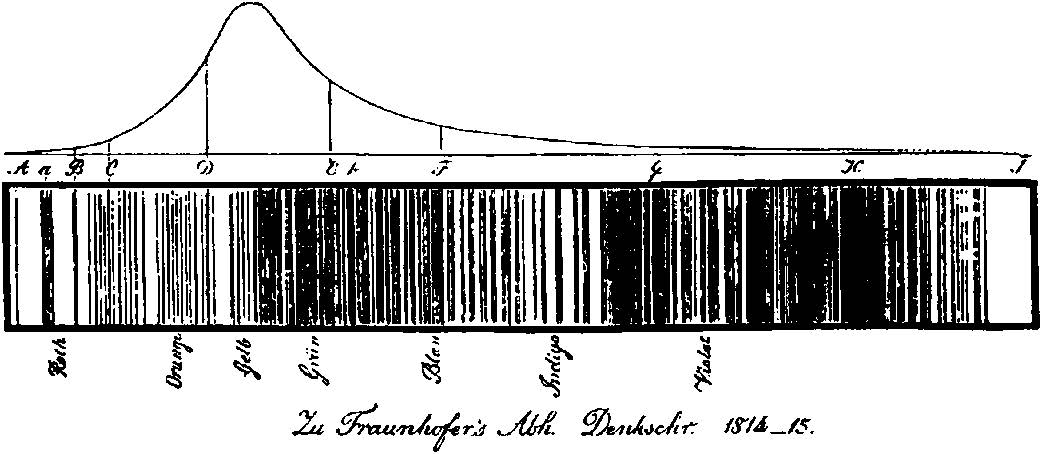
\includegraphics[width=1\textwidth]{figures/intro/Fraunhofer_lines.jpg}}{}{\label{fig:Fraunhofer_lines_old}}
    \vfill
    \Subfigure[0.7]{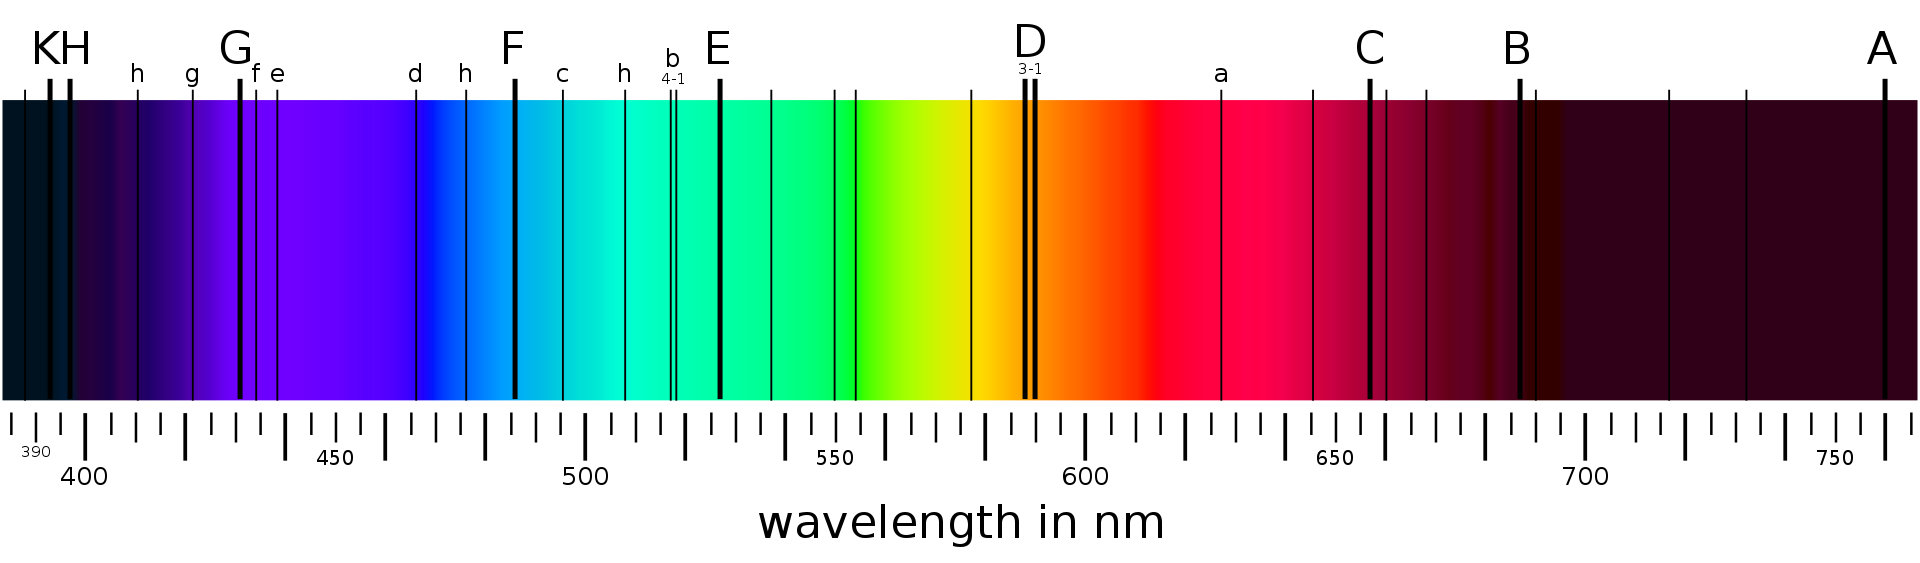
\includegraphics[width=1\textwidth]{figures/intro/Fraunhofer_lines_modern.png}}{}{\label{fig:Fraunhofer_lines_modern}}
    \vfill
    \caption{The optical spectrum of the sunlight. (a) is the original recorded spectrum (Credit: \citet{fraunhofer_first_1817}) while (b) is the same visible spectrum but coloured, from 380 nm to 710 nm (Credit: Wikimedia Commons).} 
    \label{fig:Fraunhofer_lines}
\end{figure}

\citet{fraunhofer_first_1817} used one of the first optics (the same optics that made parallax measurements possible see above) built in 1814 to reflect a ray of sunshine from a slit into a shutter onto a whitewashed wall. 
He noticed that the Sun's light was not a continuous spectrum of colours as observed by Newton \cite{newton_new_1993} 
(see Figure \ref{fig:Fraunhofer_lines}) but a series of dark lines. These lines would later become known as Fraunhofer 
lines. Fraunhofer investigated these lines further and recorded precise positions and intensities 
carefully. As a result, Fraunhofer recorded the first-ever high-resolution astronomical spectrum.
% As shown in Figure \ref{fig:Fraunhofer_lines}, in addition to the rainbow's distinctive colours, which have been observed since Newton \cite{newton_new_1993}, he noticed numerous dark lines. He meticulously recorded the precise wavelength of each dark line, now referred to as Fraunhofer lines, and assigned letters to the strongest ones. As a result, Fraunhofer recorded the first-ever high-resolution astronomical spectrum.

However, he could not determine the origin of the dark patterns he saw. When he conducted a similar experiment using light from the nearby red star Betelgeuse, he discovered that the dark lines he had observed before had significantly altered. Fraunhofer concluded that most of those characteristics were somehow connected to the nature of the object he was examining.

Nearly 45 years later, Gustav Kirchhoff and Robert Bunsen's \cite{kirchhoff_chemical_1860} (1860) experiments helped to understand Fraunhofer's observations. They investigated the colour of the light emitted as metals burned. In certain conditions, they discovered, the wavelength of the produced light matched the Fraunhofer lines. These experiments demonstrated that the atomic constitution of the Sun is the origin of the observation of the Fraunhofer lines. 

\subsection{Beyond stars}
Until the mid-20th century, in the interstellar medium (ISM), the formation and stability of molecules and the efficiency of chemical reactions were assumed to be impossible. The intense radiation and high-energy particles present in space, as well as the extremely low densities (at maximum reaching $10^6 - 10^7$ \percc) and temperatures ($<10$ K) \cite{harju_detection_2008}, were believed to prevent the formation and survival of molecules. For comparison, on Earth global average temperature is around $\sim 298$ K and the number density (atmosphere) amounts to $\sim 10^{19}$ \percc. Therefore, it was generally believed that most matter in space would appear in the form of atoms or amorphous dust grains rather than individual molecules.

\begin{figure}[!htb]
    \centering
    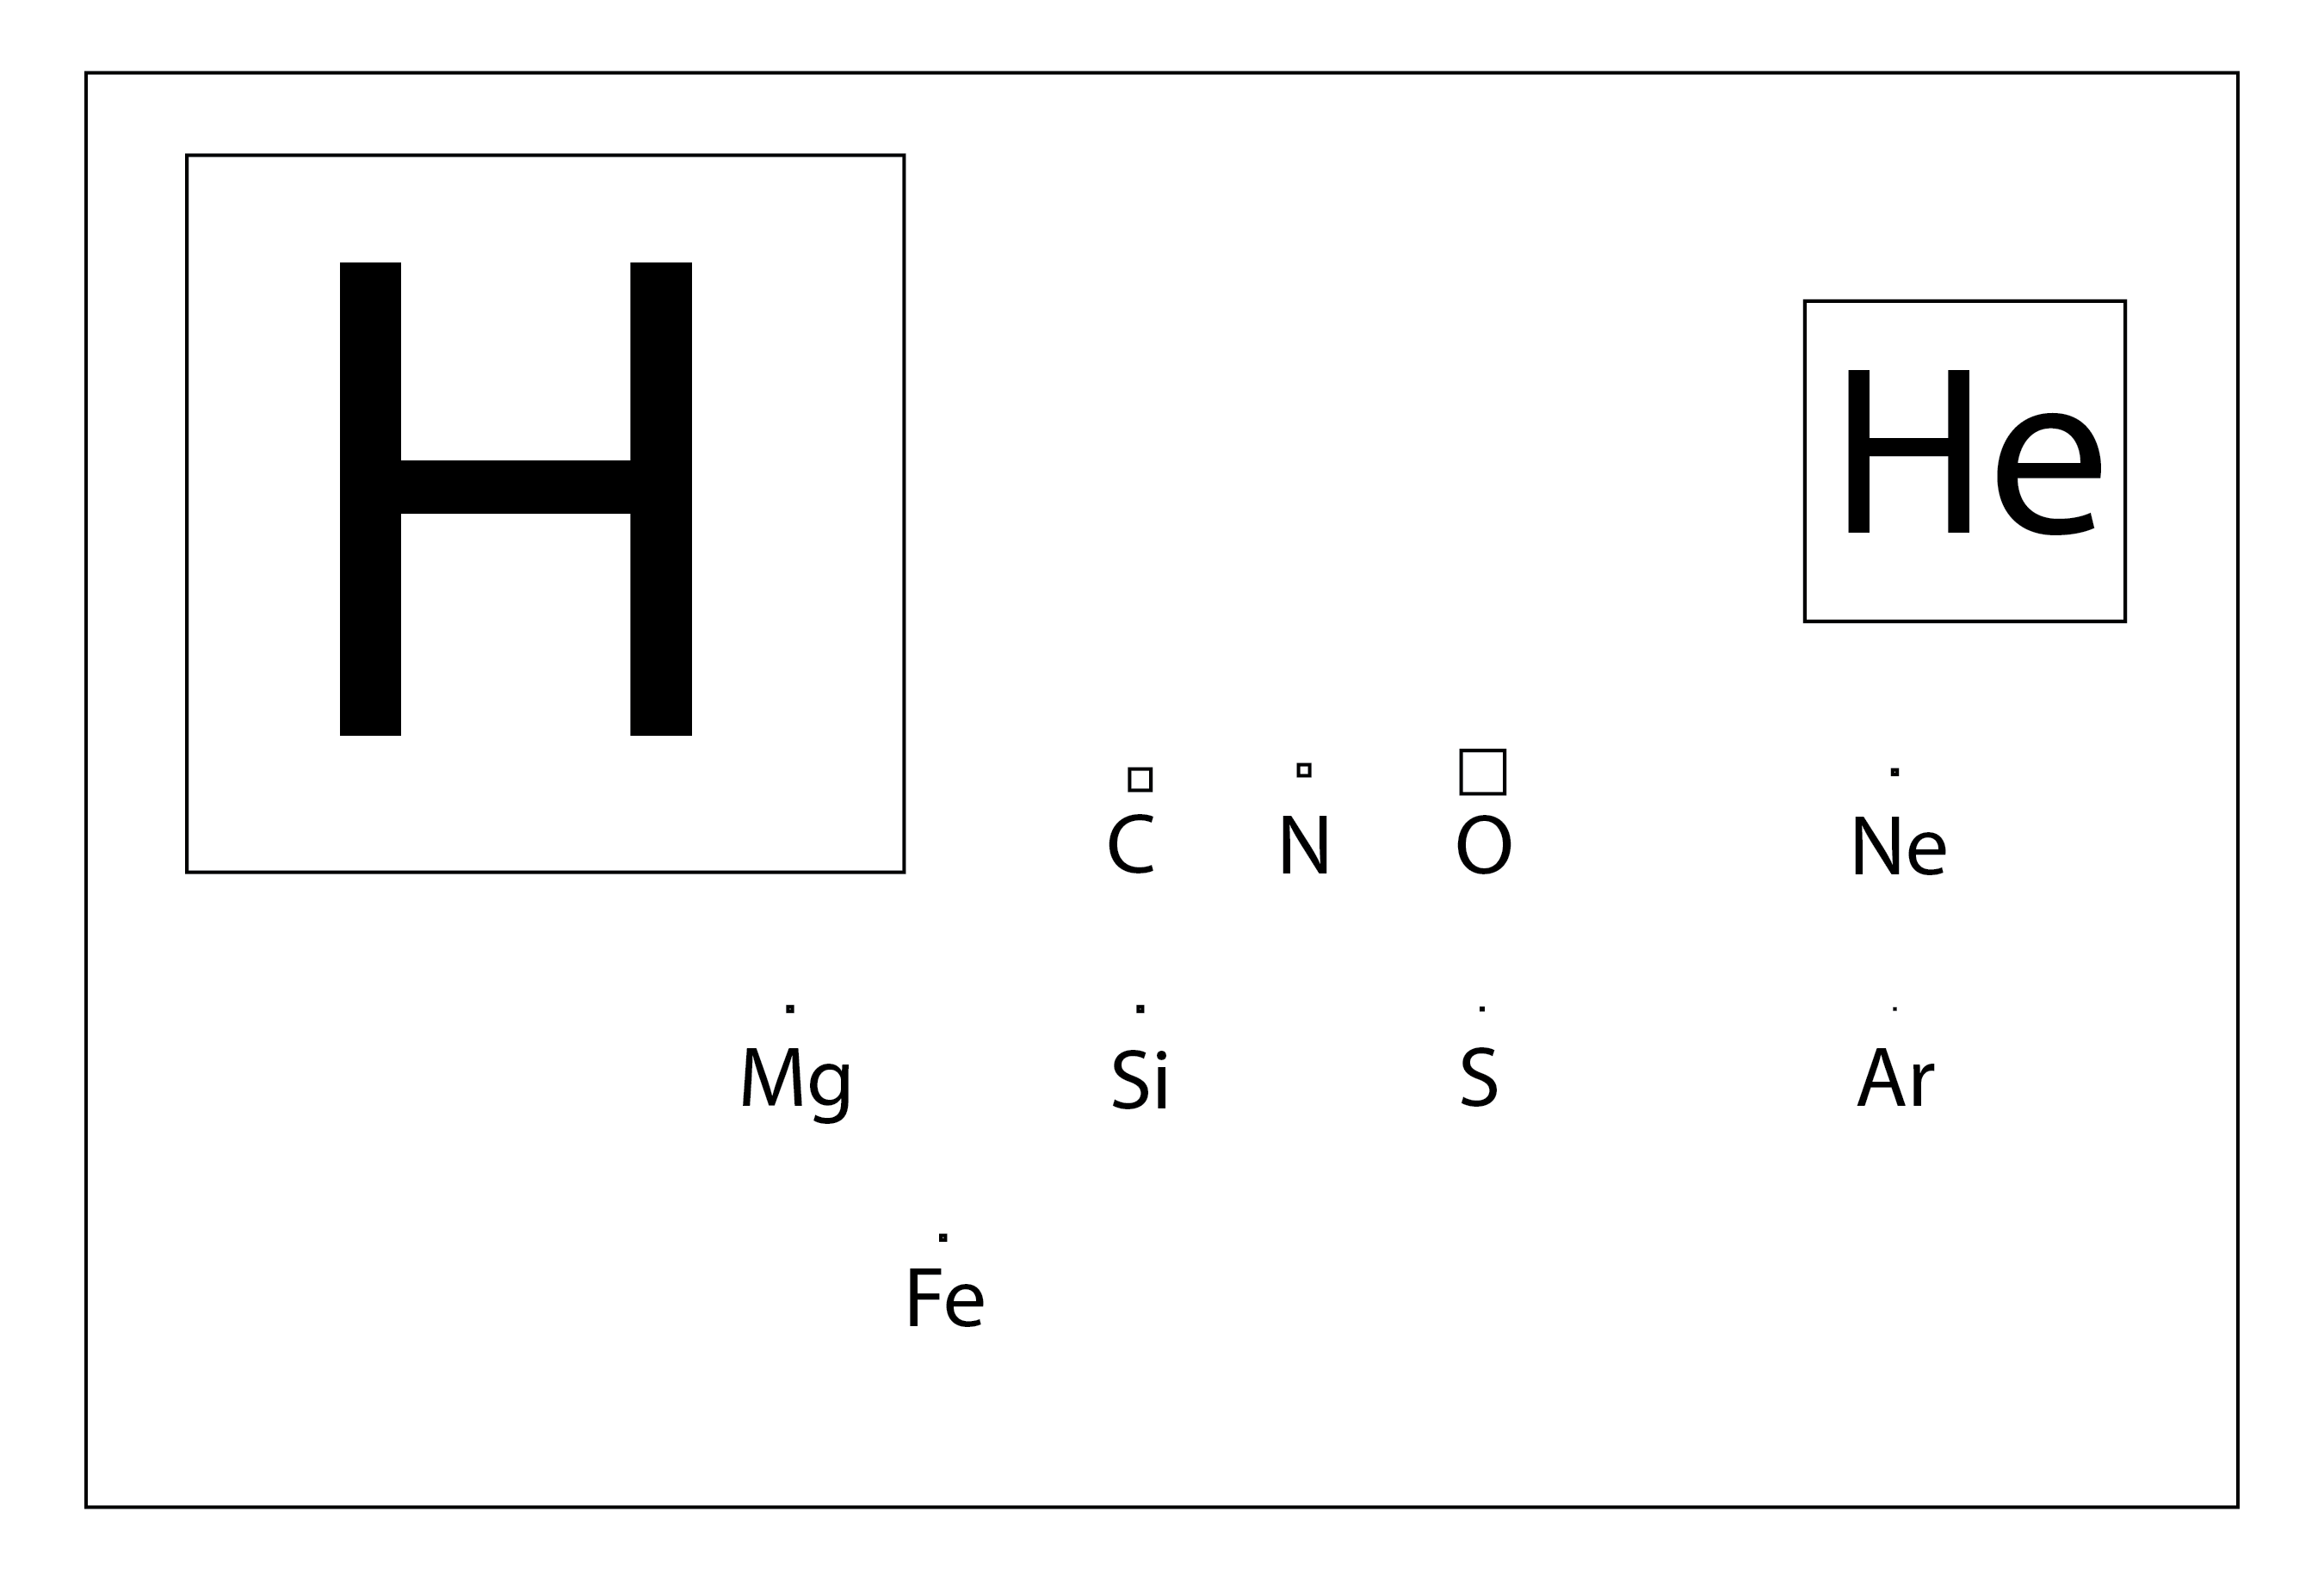
\includegraphics[width=0.6\textwidth]{figures/intro/astro-periodic-table.png}
    \caption{The Astronomer's Periodic Table, as it is referred to. This figure represents the elements by boxes with areas corresponding to their cosmic abundances. Figure adapted from \citet{mccall_optical_2005}.}
    \label{fig:astrochemistry-astro-periodic-table}
\end{figure}

Most astrophysical environments possess very low densities of gases. However, even if densities are high, H and He are 
the primary elements accessible for chemistry (see Figure \ref{fig:astrochemistry-astro-periodic-table}), which was 
thought to limit the complexity of potential chemical reactions significantly. Fortunately, the emergence of 
telescopes, detectors, and spectrometers operating in the radio, infrared (IR), and ultraviolet (UV)/visible regions of 
the electromagnetic spectrum proved this consideration incorrect. Indeed, low densities and extreme temperatures (both 
high and low) in space frequently constrain chemistry, but the vast quantities of matter and long timescale compensate 
for it. Interstellar space represents a unique laboratory in which fundamental molecular processes can be investigated 
under conditions distinctly different from Earth's.

In the following sections, a brief introduction is given to the discovery of molecules in space and the laboratory 
spectroscopic techniques that allow us to study molecular ions under interstellar conditions.

\section{Molecules in space}
\label{sec:intro:ions_in_space}

\epigraph{Somewhere, something incredible is waiting to be known}{Carl Sagan}
Sir Arthur Stanley Eddington's Bakerian Lecture on \enquote{\emph{Diffuse matter in interstellar space}} \cite{eddington_bakerian_1926} of 1926 may be a natural starting point for the discussion of molecules in the interstellar medium. The sharp calcium spectral line observed by \citet{hartmann_investigations_1904} in 1904 and the subsequent discovery of D-lines of sodium (\citet{heger_occurrence_1919} in 1919) and H and K lines of calcium (\citet{plaskett_h_1923} in 1923) were the premises of Eddington's discussion. These lines were not arising from absorption in either the stellar atmosphere or Earth's atmosphere. Since they were also unaffected by stellar motion, they were known as \emph{fixed} or \emph{stationary} lines. These lines were assumed to originate from interstellar space. Eddington pointed out in his lecture that \enquote{...it is difficult to admit the existence of molecules in interstellar space because when once a molecule becomes dissociated, there seems no chance of the atoms joining up again}. 

\subsection{Optical observation}
\label{subsec:intro:optical}

In the early 1930s, \citet{merrill_unidentified_1934} identified several interstellar lines (much wider than interstellar atomic lines) of unknown origin. \citet{russell_analysis_1935} conjectured that the origin of these lines was molecular rather than atomic. \citet{merrill_stationary_1936} noted that \enquote{the chemical identification of these lines had not been made yet}, and remarkably, the chemical identity is unknown even today for these \emph{diffuse interstellar bands} (DIBs). An exception is C$_{60}^+$ which is the only species identified as the carrier of two DIBs by \citet{campbell_laboratory_2015} only recently in 2015, based on laboratory action spectroscopic methods similar to the ones described in this thesis. However, hundreds of DIBs remain to be identified. Hence, it remains the oldest unsolved problem in astronomical spectroscopy. Nevertheless, it became clear that the interstellar absorption lines could not all be due to neutral or ionized atoms.

Later, in the late 1930s, Adams, Dunham and McKellar established the presence of CH, CN and CH$^+$ molecular species in the interstellar medium based on four sharp absorption lines seen in the optical spectra of several distant stars using Mount Wilson Observatory (\citet{dunham_jr_interstellar_1937} 1937, \citet{adams_quoted_1937} 1937, \citet{mckellar_evidence_1940, mckellar_wave_1940} 1940) and laboratory data (\citet{jenkins_mass_1938, douglas_note_1941, douglas_band_1942}). Three interstellar molecules were identified in four years, one of which was a positively charged ion. Detailed quantitative studies by \citet{bates_density_1951} in 1951, and its extension by \citet{solomon_formation_1972} in 1972 and \citet{herbst_formation_1973} in 1973, to understand the formation of these interstellar molecular species showed the crucial role of ion-molecule reactions.

\subsection{Radio observation}
\label{subsec:intro:radio}

The hydroxyl radical (OH) molecule has a ground state of $^2\Pi$, resembling CH. However, its optical resonance lines lie in the 3060 $\mathring{\text{A}}$ region, close to the atmosphere's edge of transmission. Due to interference from our own atmosphere's ozone absorption bands, it is challenging to observe these lines. \citet{weinreb_radio_1963} \citeyear{weinreb_radio_1963} observed the first lines of OH near radio frequency 1665 MHz, which represents a transition between the $\Lambda$ doublet components of the lowest rotational level $J=3/2$ of $^2\Pi_{3/2}$ (hyperfine structure). The radio detection of OH inspired many radio astronomers to consider the possibilities of detecting polyatomic molecule lines in the radio frequency range. \citet{cheung_detection_1968} succeeded in 1968 with NH$_3$ and shortly after with H$_2$O \cite{cheung_detection_1969}, both in emission. \citet{snyder_microwave_1969} soon discovered formaldehyde (H$_2$CO) in absorption; numerous new compounds have been discovered annually, a trend that has continued at a nearly linear rate ever since \cite{mcguire_2021_2021}.

\subsection{Infrared observation}
\label{subsec:intro:IR}

\citet{gillett_8_1973}, using ground observations, discovered three distinct emission bands in the 8 - 14 $\mu$m spectra of two planetary nebulae (NGC), ushering in a new era in astrochemistry in the early 1970s \cite{li_spitzers_2020}. 
Followed by \citet{merrill_2_1975}, detecting a broad emission band in NGC 7027.
During this period, airborne observations became feasible for the first time, enabling the Kuiper Airborne Observatory (KAO) to identify two new powerful emission bands in NGC 7027 and an external galaxy (M82) \cite{russell_4_1977, willner_2_1977}.
% Airborne observations also became feasible during that period for the first time. This allowed the Kuiper Airborne Observatory (KAO) to find two new powerful emission bands in NGC 7027 and an external galaxy (M82) \cite{russell_4_1977, willner_2_1977}. 
These characteristics were ubiquitous in space and closely related, forming the PAH family (PAH=Polycyclic Aromatic Hydrocarbons) \cite{li_spitzers_2020}.
Despite being widely observed, the precise nature of the carriers of these features remains elusive, and they are currently referred to as unidentified infrared emission (UIE) features.
% Although the precise nature of the carriers of these features is still unknown, they have been collectively referred to as unidentified infrared emission (UIE) features. 
However, the hypothesis that PAH molecules serve as carriers have received significant support \cite{leger_identification_1984, allamandola_polycyclic_1985}. The PAHs in ISM are postulated to be 
assembled by smaller molecules, and smaller molecular ions play an important role as an intermediate 
and the main driving force of interstellar chemistry \cite{smith_ion_1992,herbst_dense_1988,CGP2015}.

\begin{figure}[!htb]
    \centering
    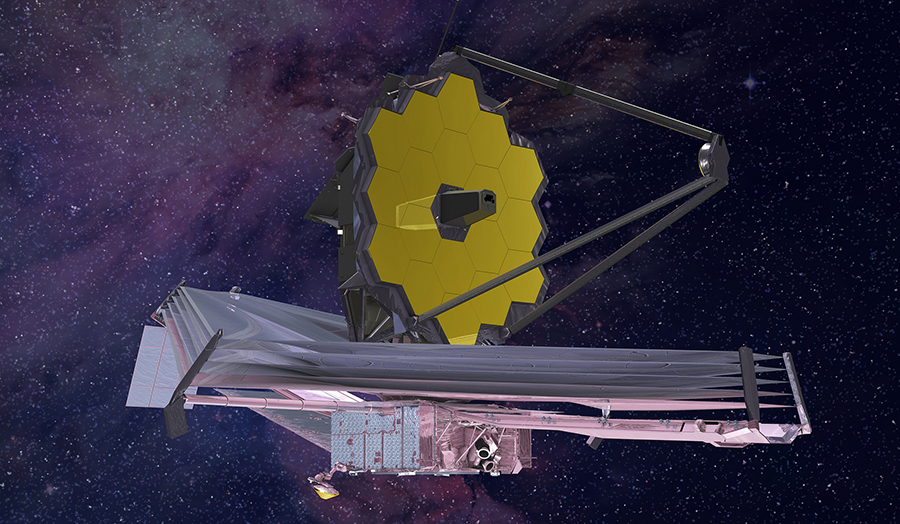
\includegraphics[scale=0.3]{figures/intro/JWST.jpg}
    \caption{James Webb Space Telescope - An infrared-optimized astronomical observatory (Credit: NASA)}
    \label{fig:JWST}
\end{figure}

Recently, the James Webb Space Telescope (JWST), as shown in Figure \ref{fig:JWST} was launched in late 2021. It is an infrared-optimized astronomical observatory that operates in near- ($0.6 - 5$ $\mu$m) and mid- ($5 - 28$ $\mu$m) infrared regions \footnote{\url{https://www.jwst.nasa.gov/content/observatory/instruments/index.html}} to address a range of astrophysical and cosmological questions, including the role of PAHs.

\subsection{Current status}
Astronomers are now aware of many additional diatomic and polyatomic molecules in the ISM. Furthermore, a large number of unknown species await their identification, such as the UIE and DIBs. As of early May 2023, about 295 molecules have been detected in the ISM or circumstellar shells (CDMS database\footnote{\url{https://cdms.astro.uni-koeln.de/classic/molecules}}), and $\sim 12 \%$ of them are cationic species \cite{mcguire_2021_2021} see Figure \ref{fig:ISM_molecules}. Interstellar molecules can be identified through their electronic (optical), vibrational (infrared), and rotational (radio) spectra as shown in Sections \ref{subsec:intro:optical} through \ref{subsec:intro:IR}. However, most ($\sim$ 80 \%) of interstellar species are identified via their rotational transition \cite{mcguire_2021_2021} because of their low excitation temperature and distinct spectroscopic  fingerprint. In conclusion, one can say that laboratory spectroscopic data are indeed vital in identifying these molecular species in space. This is difficult for highly reactive molecular ions, but their laboratory characterization and subsequent astronomical detection are important to understand the ion-molecule chemistry of the ISM. Therefore, in the next section, a brief introduction to spectroscopy followed by a detailed review of spectroscopic methods especially for studying molecular ions are presented.

\begin{figure}[!htb]
    \centering
    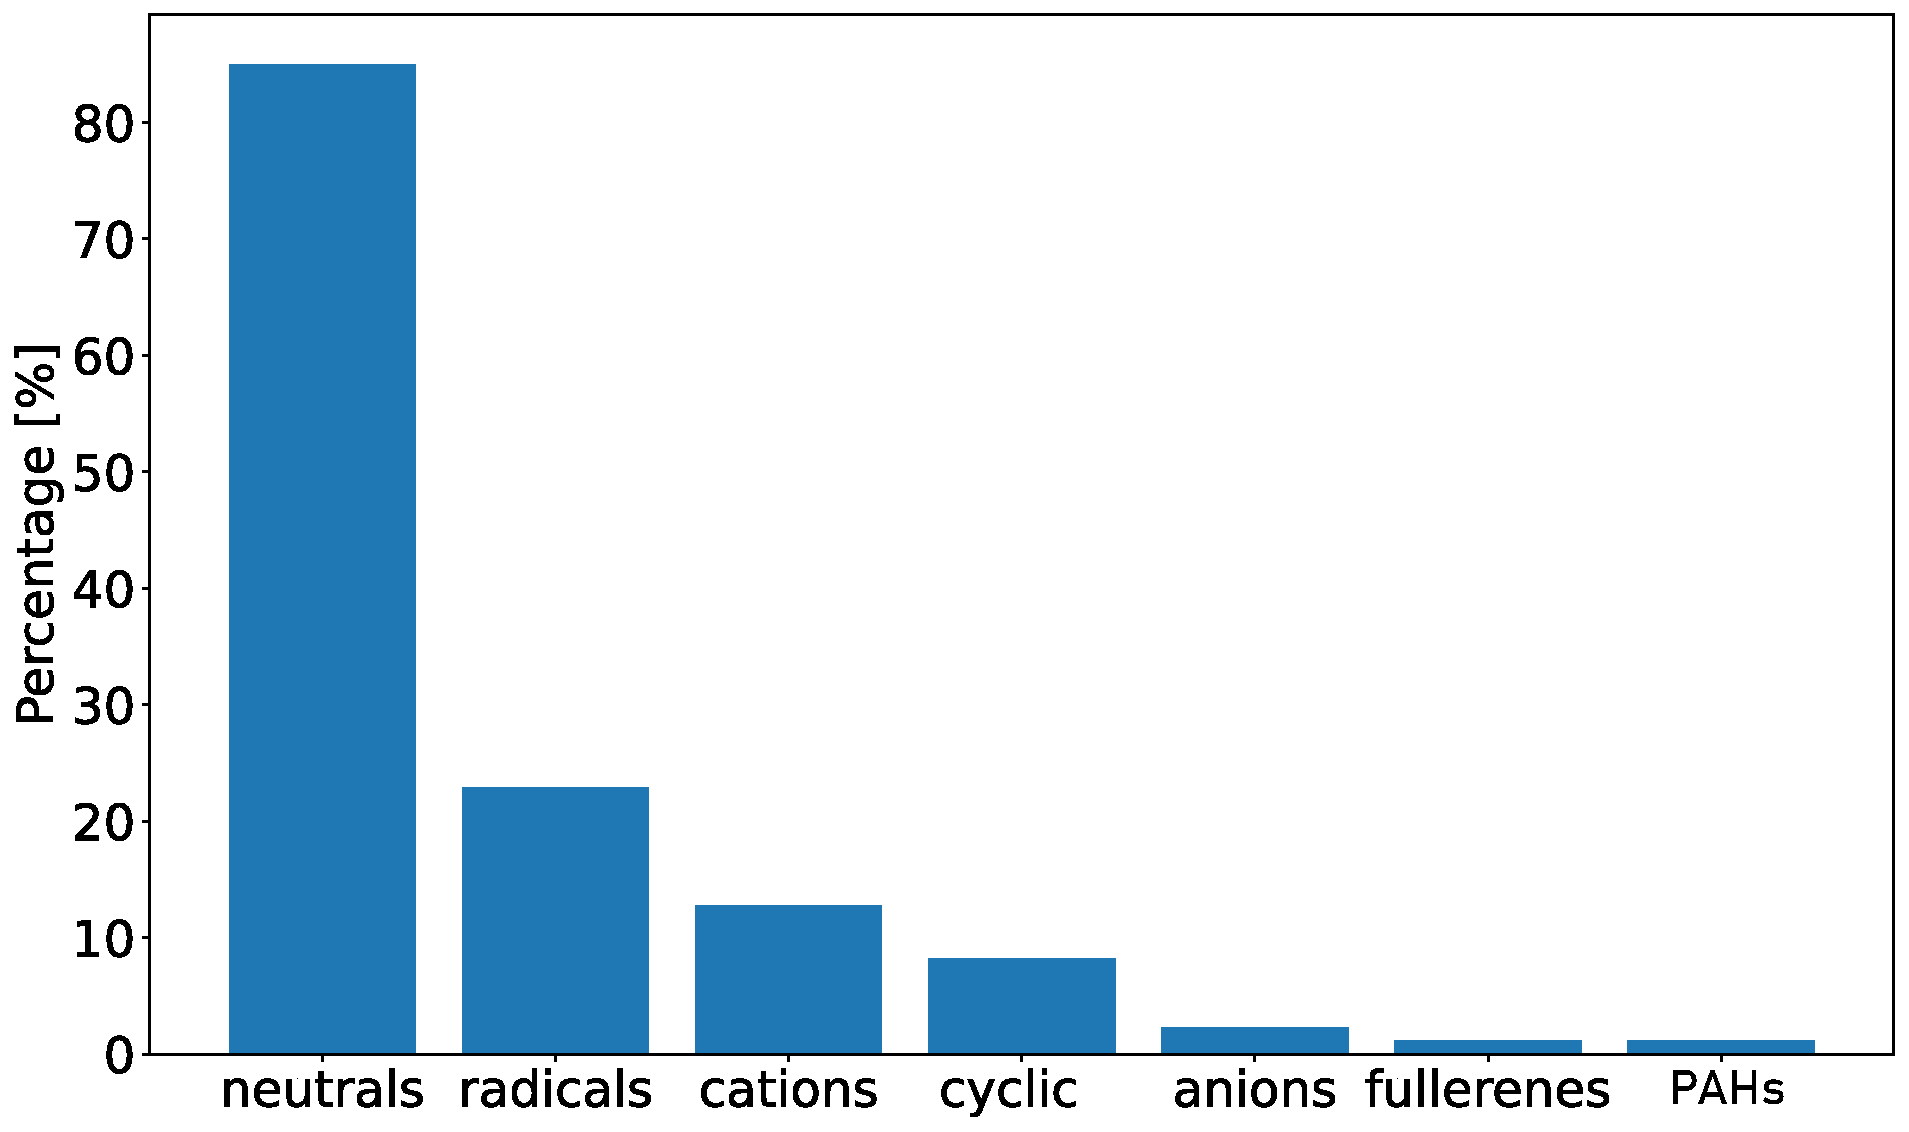
\includegraphics[width=0.75\textwidth]{figures/intro/known_molecules_in_space.pdf}
    \caption{Percentage of different classes of  known interstellar molecules. Many molecules fall into more than one of these categories \emph{e.g.} most radical species have a net neutral charge. Data is computed using \emph{astromol - A Database of Molecules Detected in Space} python library \cite{mcguire_astromol_2021}}
    \label{fig:ISM_molecules}
\end{figure}

\section{Spectroscopy}
\label{sec:spectroscopy}

The Light of Knowledge is a common expression, but it fits especially in the
spectroscopy context. Spectroscopy is the broad field of study that measures
and interprets the interaction between matter and electromagnetic radiation
as a function of wavelength or frequency. Most of our knowledge regarding atoms and molecules 
comes from examining their interactions with electromagnetic radiation; 
as a result, various parts of the electromagnetic spectrum supply
different types of information (see Figure \ref{fig:EM_spectrum}). The
molecular transitions, such as rotational, vibrational and electronic excitation, 
are characterized via interactions in different regions of the electromagnetic
spectrum, as shown in Table \ref{tab:electromagnetic_spectrum}. Spectroscopic
characteristics are like molecular fingerprints.

\begin{figure}[!htb]
    \centering
    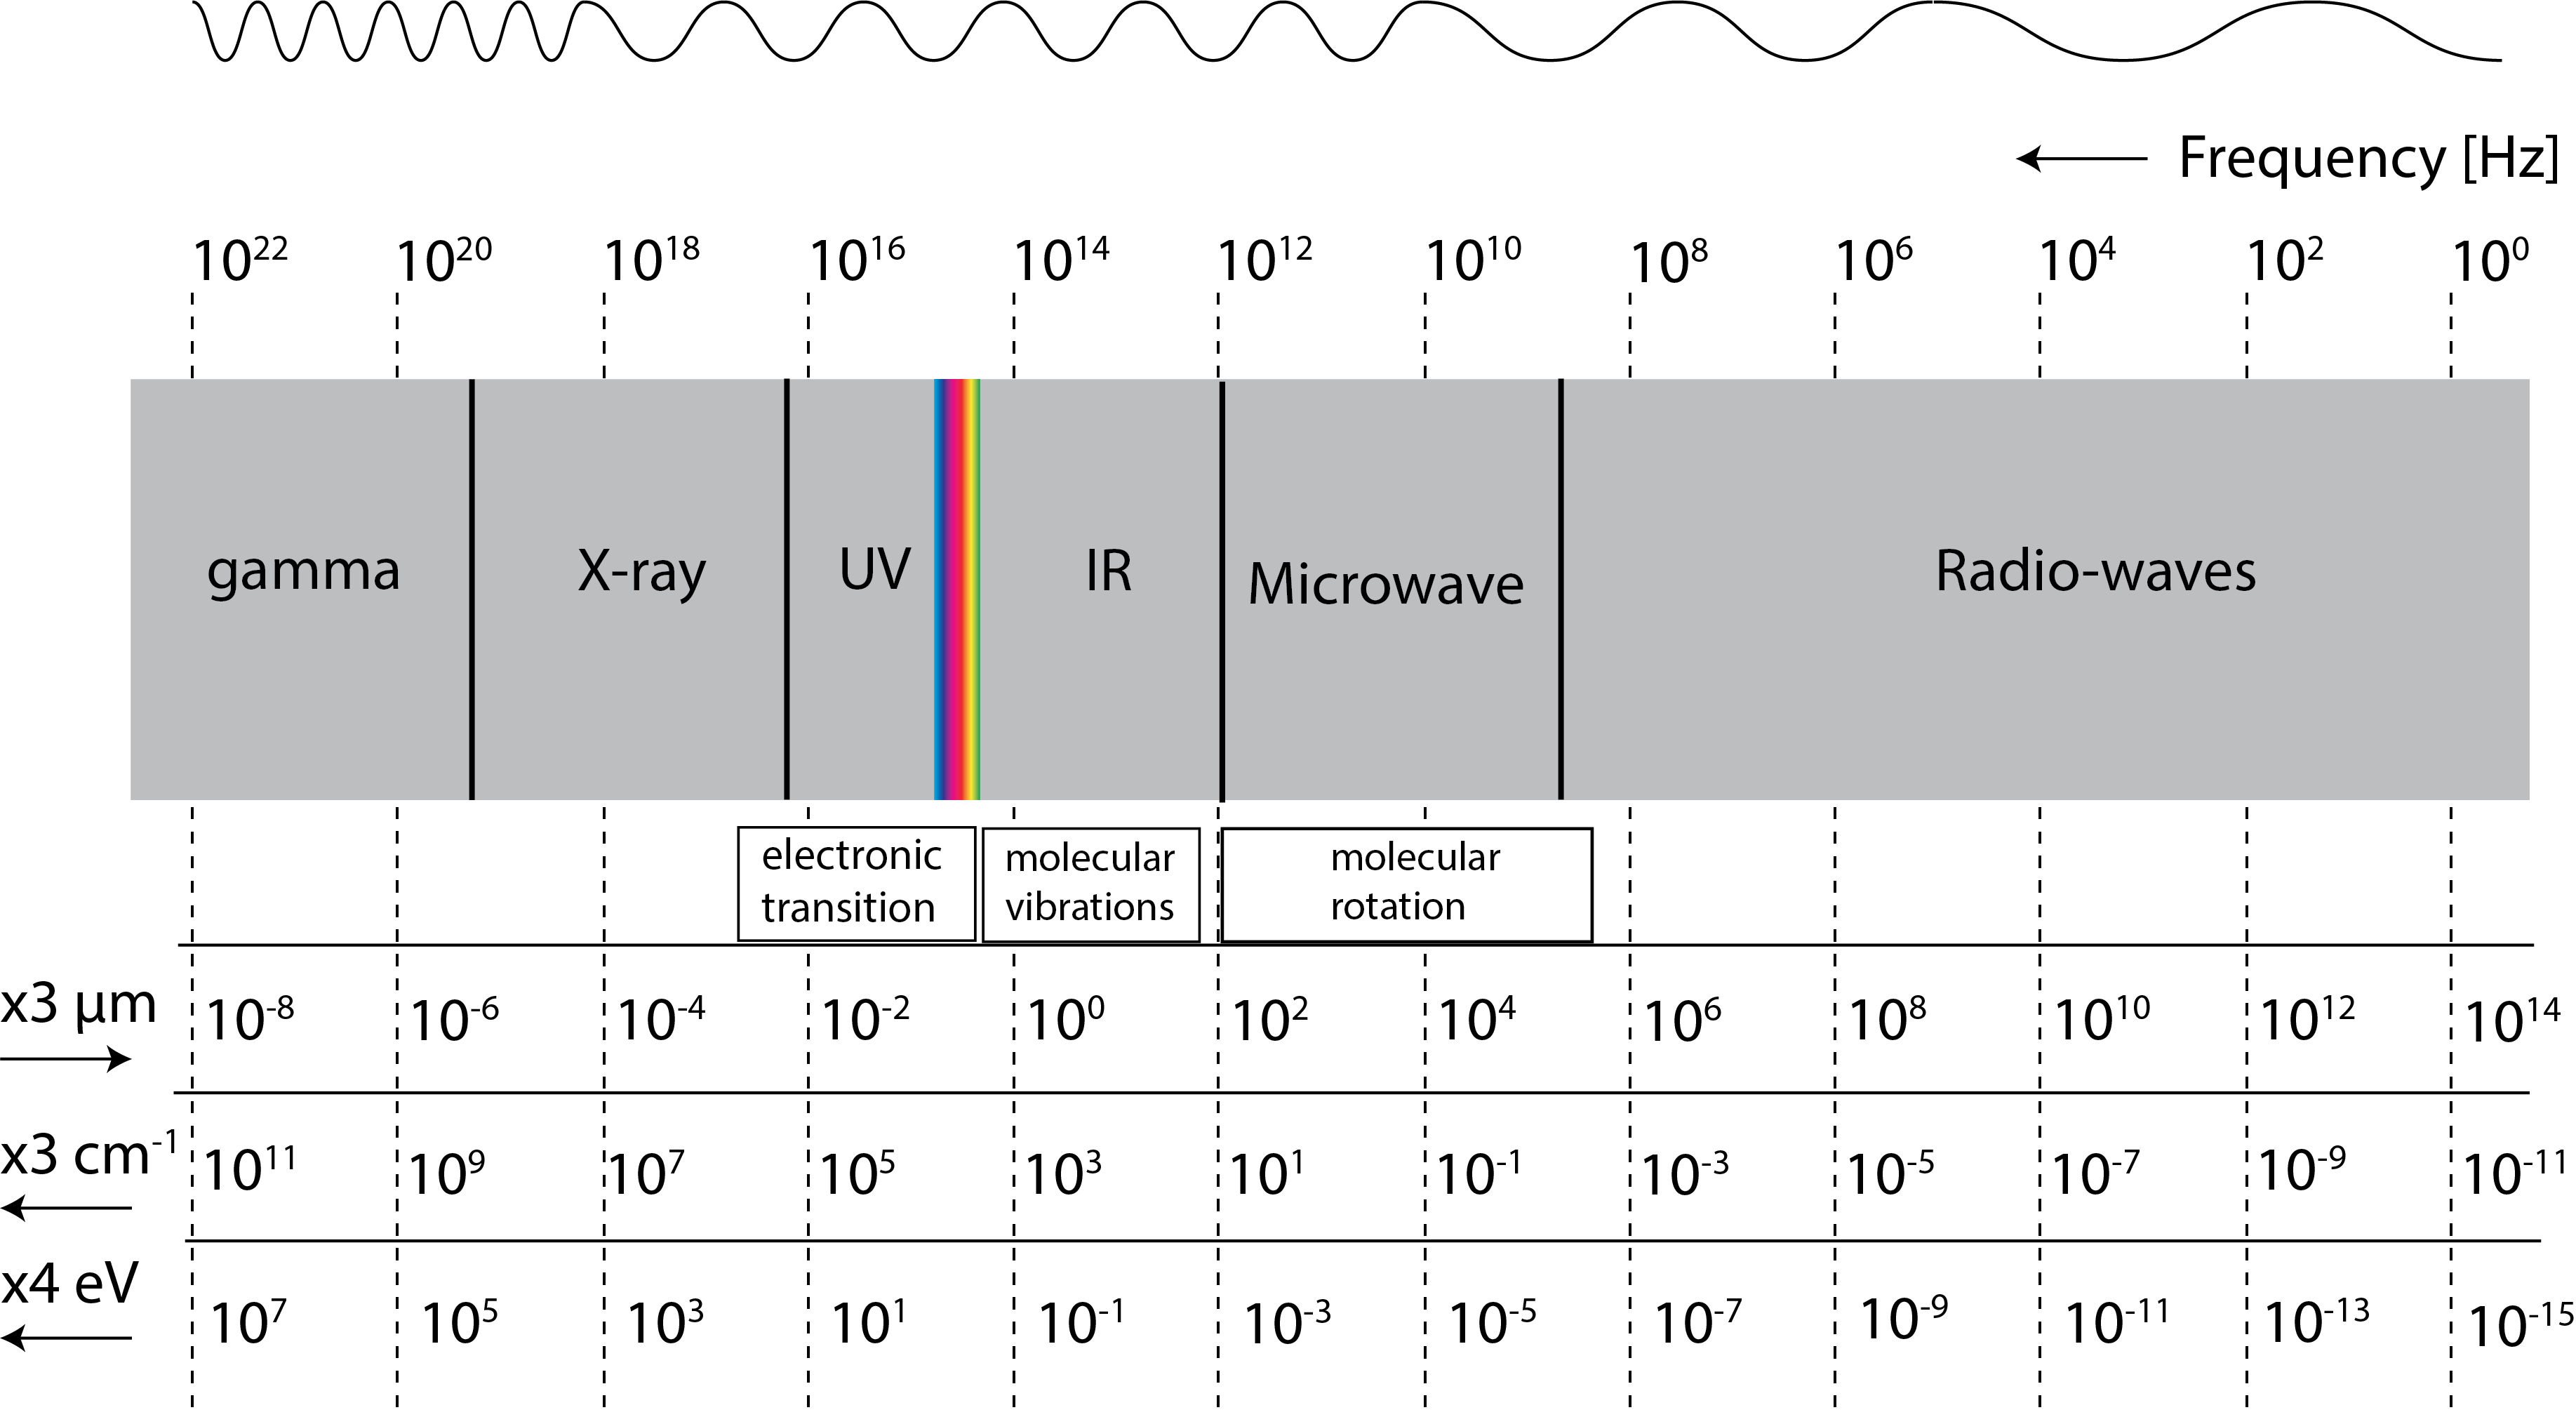
\includegraphics[width=0.9\textwidth]{figures/intro/EM_spectrum_1.png}
    \caption{Schematic diagram of the electromagnetic spectrum, the rainbow-coloured inset shows the visible spectrum. The vertical dashed line indicates a corresponding comparison to the different unit systems as labeled on the left, and \qt{x3} and \qt{x4} indicate that the scale value is multiplied by factors 3 and 4, respectively.}
    \label{fig:EM_spectrum}
\end{figure}

\begin{table}[!htb]
    \centering
    \caption{Dominant types of molecular transitions in each region of the electromagnetic spectrum}
    \begin{tabular}{lccc}
        \toprule
        \multicolumn{2}{c}{\textbf{Region of Spectrum}} & \textbf{Energy [cm$^{-1}$]} & \textbf{Molecular transitions} \\\midrule
        \multicolumn{2}{c}{\emph{Ultraviolet (UV)}} && \multirow{4}*{Electronic}\\
        & far & $10^6 - 50,000$ & \\
        & near & $50,000 - 26,300$ & \\
        \addlinespace
        \multicolumn{2}{c}{\emph{Visible (Vis)}} & $26,300 - 12,800$ & \\
        \midrule\addlinespace
        \multicolumn{2}{c}{\emph{Infrared (IR)}} && \multirow{4}*{Vibrational} \\
        & near & $12,800 - 4000$ & \\
        & mid  & $4000 - 200$ & \\
        & far  & $200 - 10$ & \\
        \midrule\addlinespace
        \multicolumn{2}{c}{\emph{Microwave (THz)}} & $10 - 0.01$ & Rotational \\
        \bottomrule\hline\\
    \end{tabular}
    \label{tab:electromagnetic_spectrum}
\end{table}


Spectrochemical analysis was invented in 1860 by
\citet{kirchhoff_chemical_1860}, but it saw limited use until the 1930s. Since
the discovery of the first molecules in space by their optical spectra, i.e.,
CN and CH \cite{dunham_jr_interstellar_1937, adams_quoted_1937,
    mckellar_evidence_1940, mckellar_wave_1940}, spectroscopy has been successfully
used in astronomy to identify new molecular species and determine physical and
chemical conditions such as gas excitation temperatures and chemical
abundances. Over the past two decades, spectral data has significantly increased from astronomical observations ranging from the UV-vis to the $mm$ and $cm$ wavelength region. A direct comparison with astronomical data is made possible
by laboratory spectroscopic investigations of gas-phase molecules, which has
significantly aided the interpretation of astrophysical findings (see Figure
\ref{fig:astrochemistry-flow-chart}).

\begin{figure}[!htb]
    \centering
    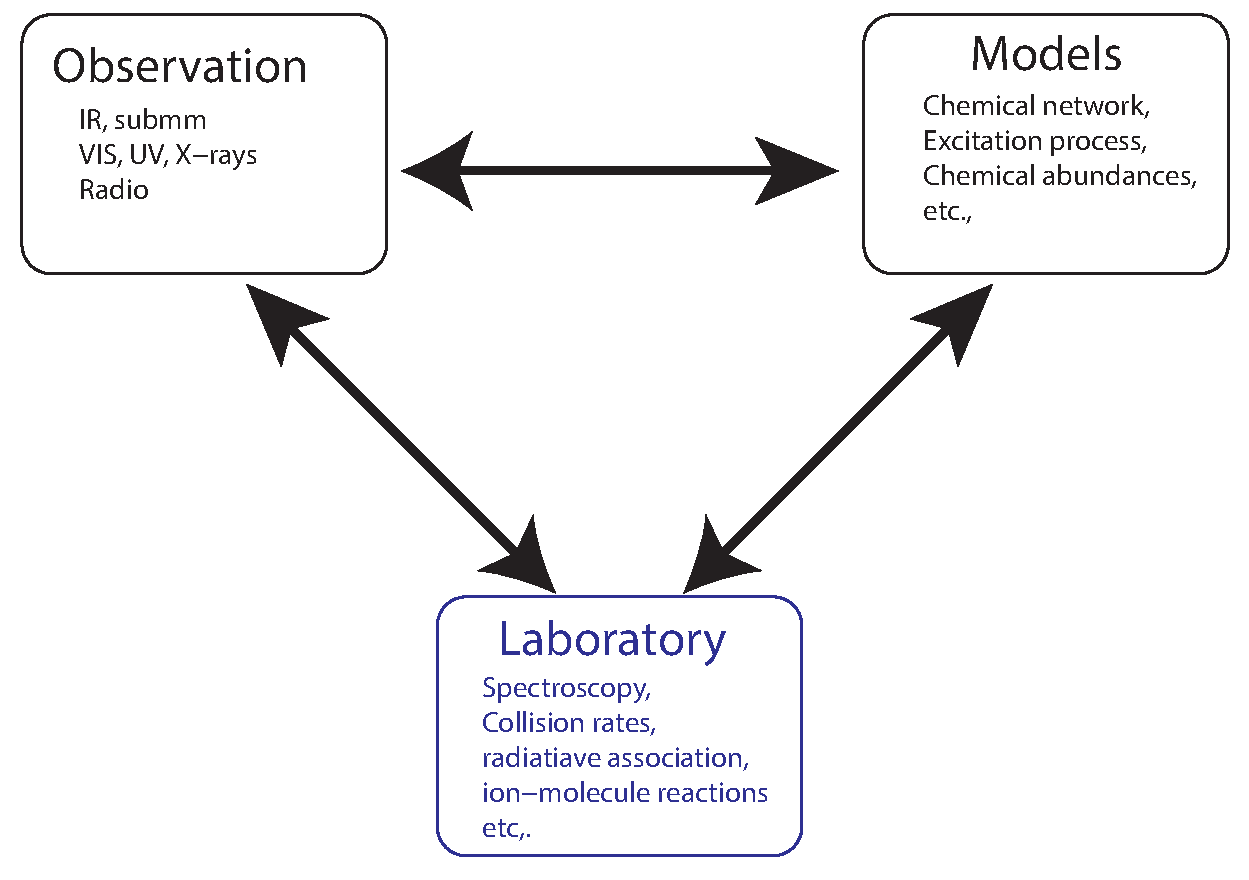
\includegraphics[width=0.8\textwidth]{figures/intro/astrochemistry-flow-chart.pdf}
    \caption{The triangular approach of observations, models, and laboratory studies is necessary to address astrochemistry questions. Examples for every category are provided in smaller fonts with respective boxes. \enquote{Laboratory} implies both experimental and theoretical work. The blue coloured box indicates the area focused on in this thesis.}
    \label{fig:astrochemistry-flow-chart}

\end{figure}

\subsubsection*{Absorption Spectroscopy}

Traditionally spectroscopic measurements of vibrational and rotational
transitions for molecules are recorded via direct absorption techniques to
detect radiation absorption as a function of frequency or wavelength due to its
interaction with the molecule sample. Since all of the atoms and molecules have
distinct and distinguishable energy levels, a measurement of the absorption
lines from incident radiation permits the identification of the absorbing
species. The absorption spectrum is the change in absorption intensity as a
function of frequency (see Figure \ref{fig:absorption_spectroscopy}).\\

\begin{figure}[!htb]
    \centering
    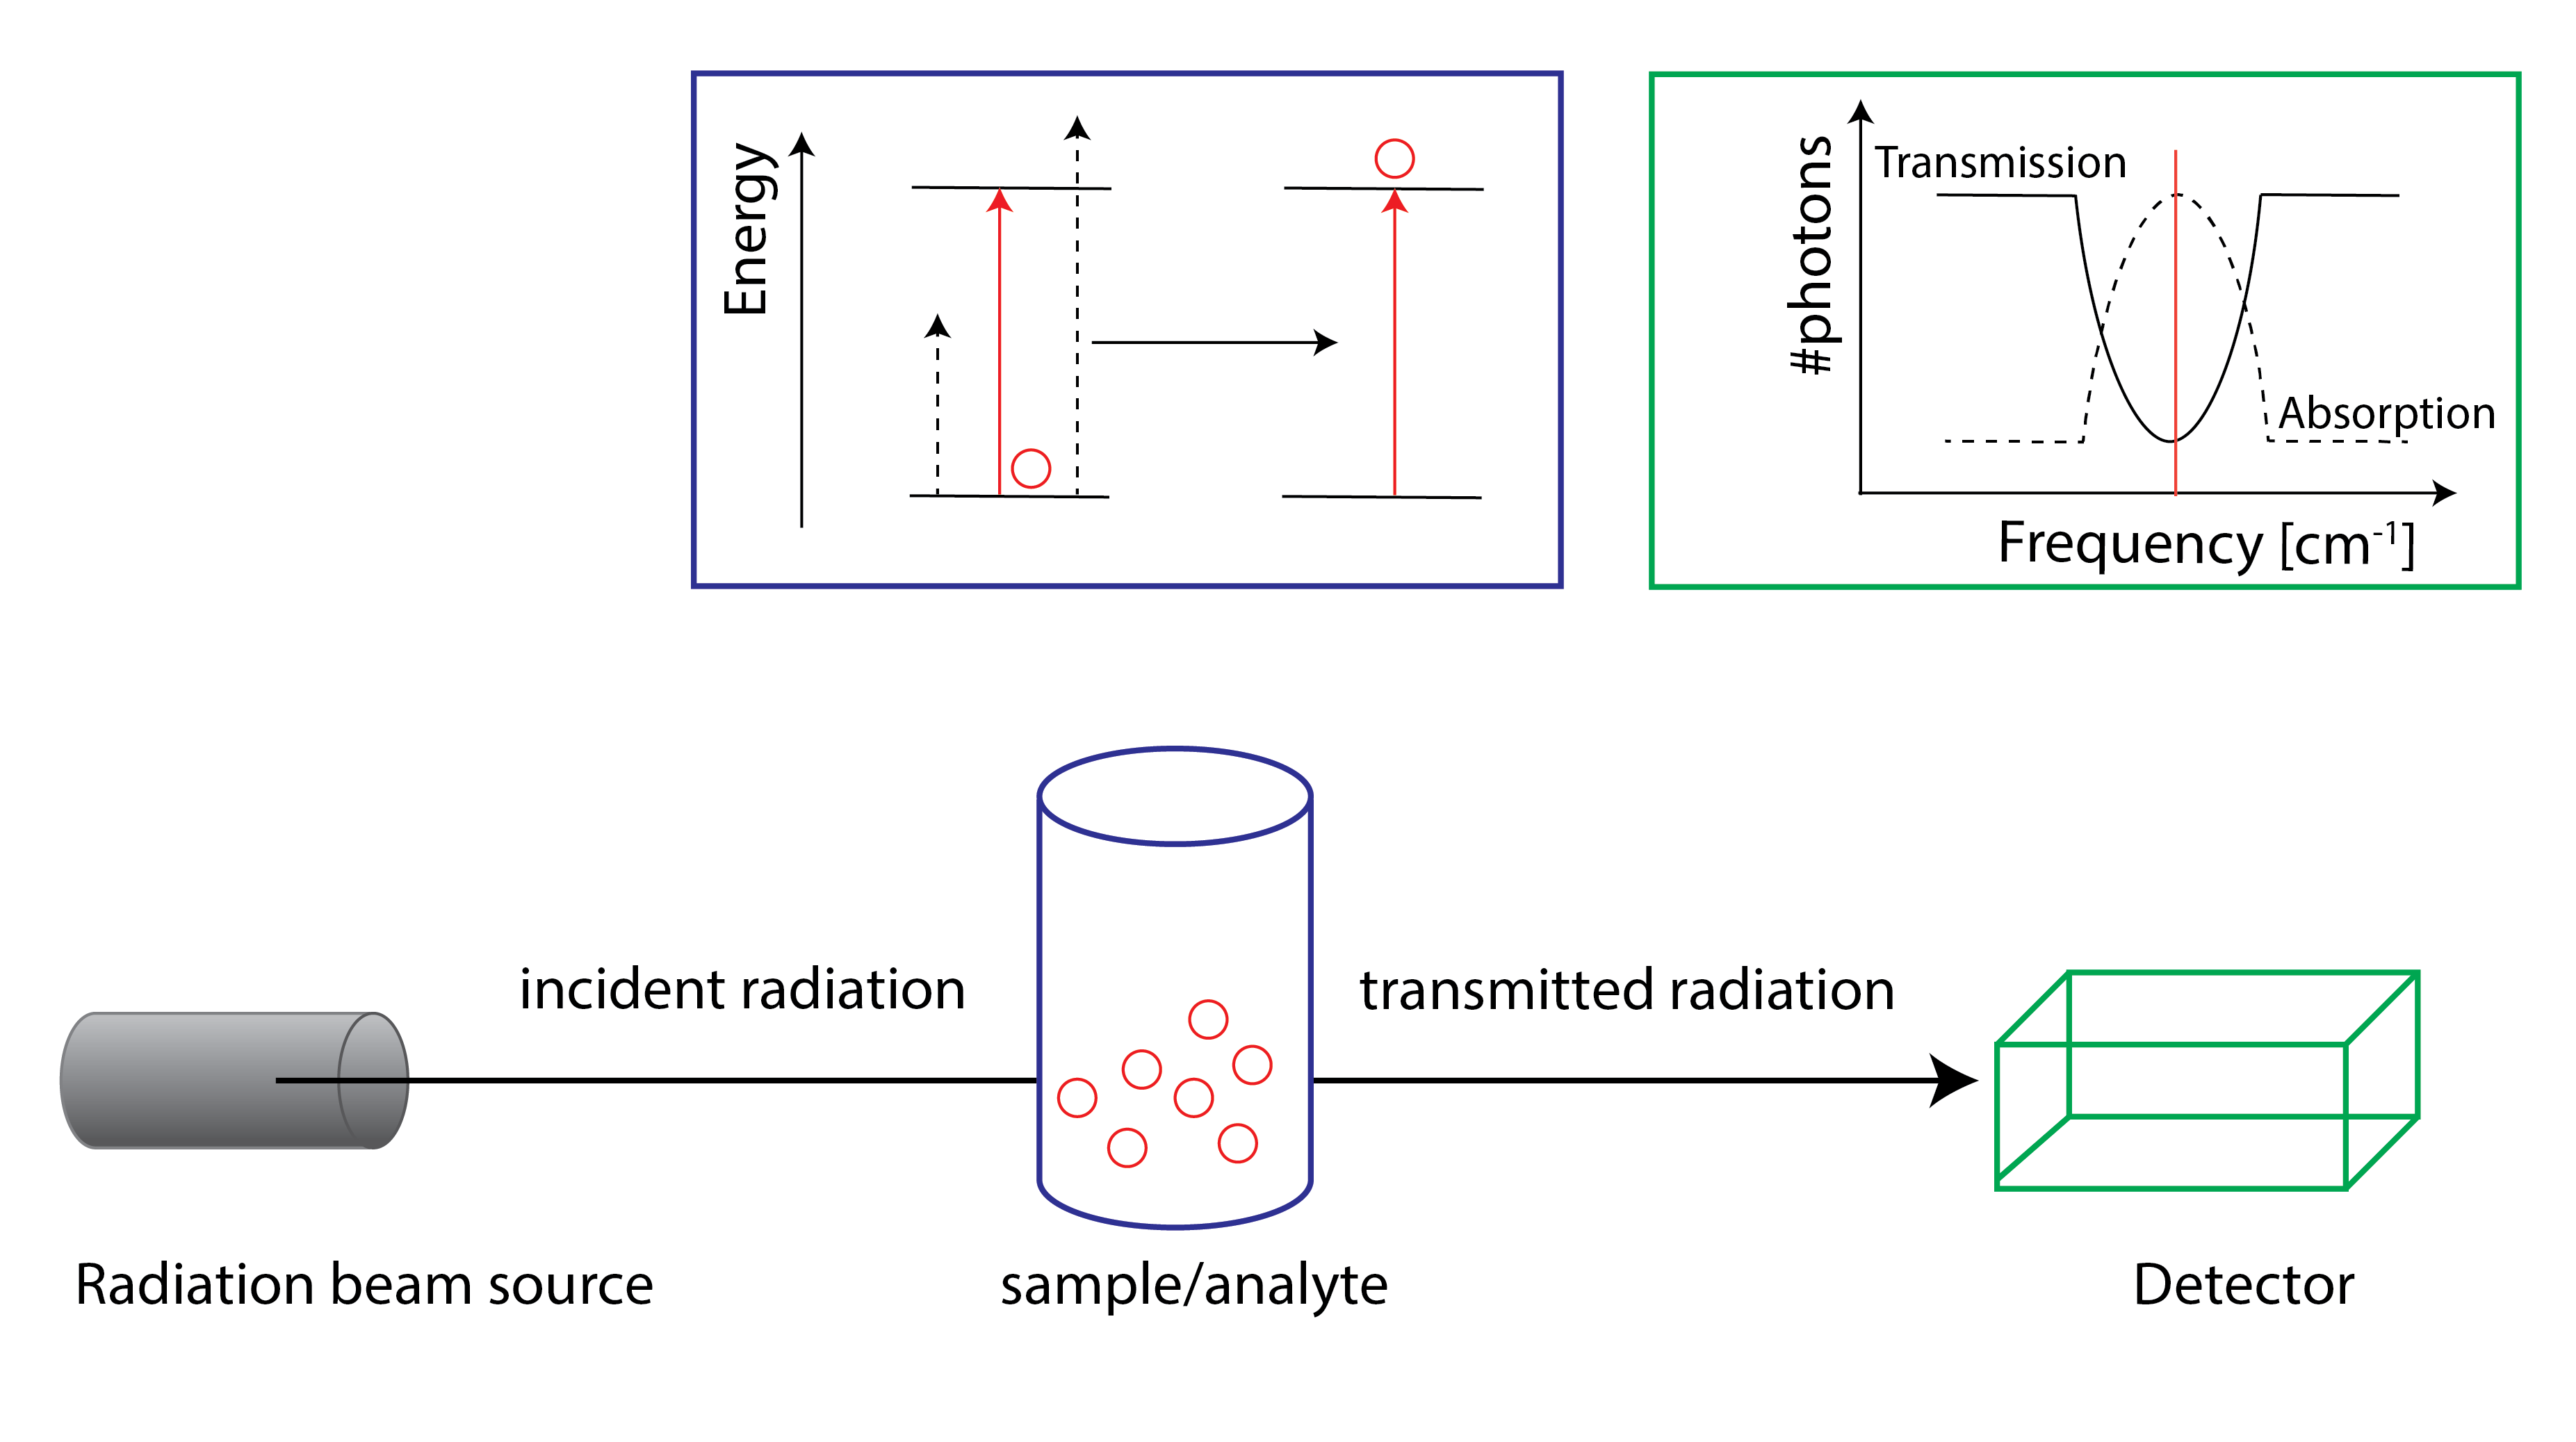
\includegraphics[width=0.8\textwidth]{figures/intro/Absorption.png}
    \caption{Schematic diagram to describe the principle of absorption spectroscopy.}
    \label{fig:absorption_spectroscopy}
\end{figure}

However, these conventional absorption techniques are very challenging to
record spectra of gas-phase molecular ions, especially of highly reactive,
open-shell species, since it is difficult to produce them in sufficient
number density. Another complication arises from background contamination from
other species during the formation process. Oka's \cite{oka_taming_2015} search
for the infrared spectrum of CH$_5^+$ using a discharge through a
CH$_4-$H$_2-$He mixture is a well-known illustration of this challenge.

\subsubsection*{Fourier-Transform Spectroscopy}

Fourier-transform spectroscopy (FTS) is a technique used in the field of spectroscopy to obtain high-resolution spectra of molecules. This technique is conceptually different from direct absorption spectroscopy. 
The FTS is based on the Fourier transform of a time-domain signal, which is obtained by 
measuring the intensity of light emitted or absorbed by the molecules as a function of time.

The FTS technique using microwave radiation is a well-known powerful tool for the study of rotational transitions of molecules, known as Fourier Transform MicroWave (FTMW) spectroscopy. In 1979 Balle and Flygare first developed the FTMW spectroscopy by combining a pulsed microwave source with a tunable high-quality Fabry-P\'erot cavity to study the rotational spectra of a weak molecular complex \cite{balle_new_1979, balle_fabryperot_1981}. The molecular sample is introduced into the cavity by supersonic expansion.

In FTMW, microwave pulse radiation excites the molecules' rotational energy levels which are subsequently probed with a high-resolution Fourier transform spectrometer, which detects the microwave radiation coherently emitted from the molecules as they relax to their original state (free induction decay).
The Pate group at the University of Virginia has developed a broadband Chirped-Pulse Fourier Transform MicroWave \text{(CP-FTMW)} spectrometer, which is capable of recording spectra with $>1000$-fold improvement in the rate at which the data can be acquired over a Fabry-P\'erot cavity pulsed FTMW \cite{brown_rotational_2006, brown_broadband_2008, park_perspective_2016}.

However, so far this method has only been applied to closed-shell molecular ions (mainly protonated and anions), and is not easily applicable to open-shell species, for the same reason as in absorption spectroscopy (see above) \cite{gottlieb_rotational_2000, mccarthy_laboratory_2006, mccarthy_laboratory_2015}. In addition, these techniques are not necessarily available for smaller molecular ions due to very high frequencies of the rotational transitions (such as $>400$ GHz as used in our study).
Therefore, another form of spectroscopy, known as action spectroscopy, is employed in this thesis study to record both the rotational and vibrational spectra of molecular ions.

\subsubsection*{Action Spectroscopy}

In action spectroscopy techniques, using sensitive mass spectrometry, a change in the chemical composition of ions is monitored when they interact with resonant radiation light instead of the absorption of photons by molecular ions.
\citet{asvany_understanding_2005} successfully employed one such technique in a
cryogenic ion trap to record the infrared spectrum of the elusive CH$_5^+$
molecular ion (see Section \ref{subsec:action:methods:vibrational:LIR} and
\ref{subsec:action:methods:vibrational:LIICG}).

Action spectroscopy can offer several advantages, such as mass selection and
storage in a cold ion trap, leading to uncontaminated spectra and narrow line
widths. In the next section, we shall discuss the cryogenic ion trap techniques
to isolate and confine molecular ions before continuing to describe action spectroscopy
techniques in more detail for vibrational and rotational transitions of molecular ions.

\section{Cryogenic ion trap}

An electric field exerts a force on a charged particle, such as an atomic or molecular ion. Earnshaw's \cite{earnshaw_nature_1848} theorem states that it is impossible to maintain stable confinement (i.e., trapping) of charged particles by static electric fields. However, it is possible to trap ions in stable confinement using time-varying (rf - radiofrequency) electric fields. Since the ions are confined in a fast oscillating rf electric field, it is also known as radiofrequency ion trapping.

\begin{figure}[!htb]
    \centering
    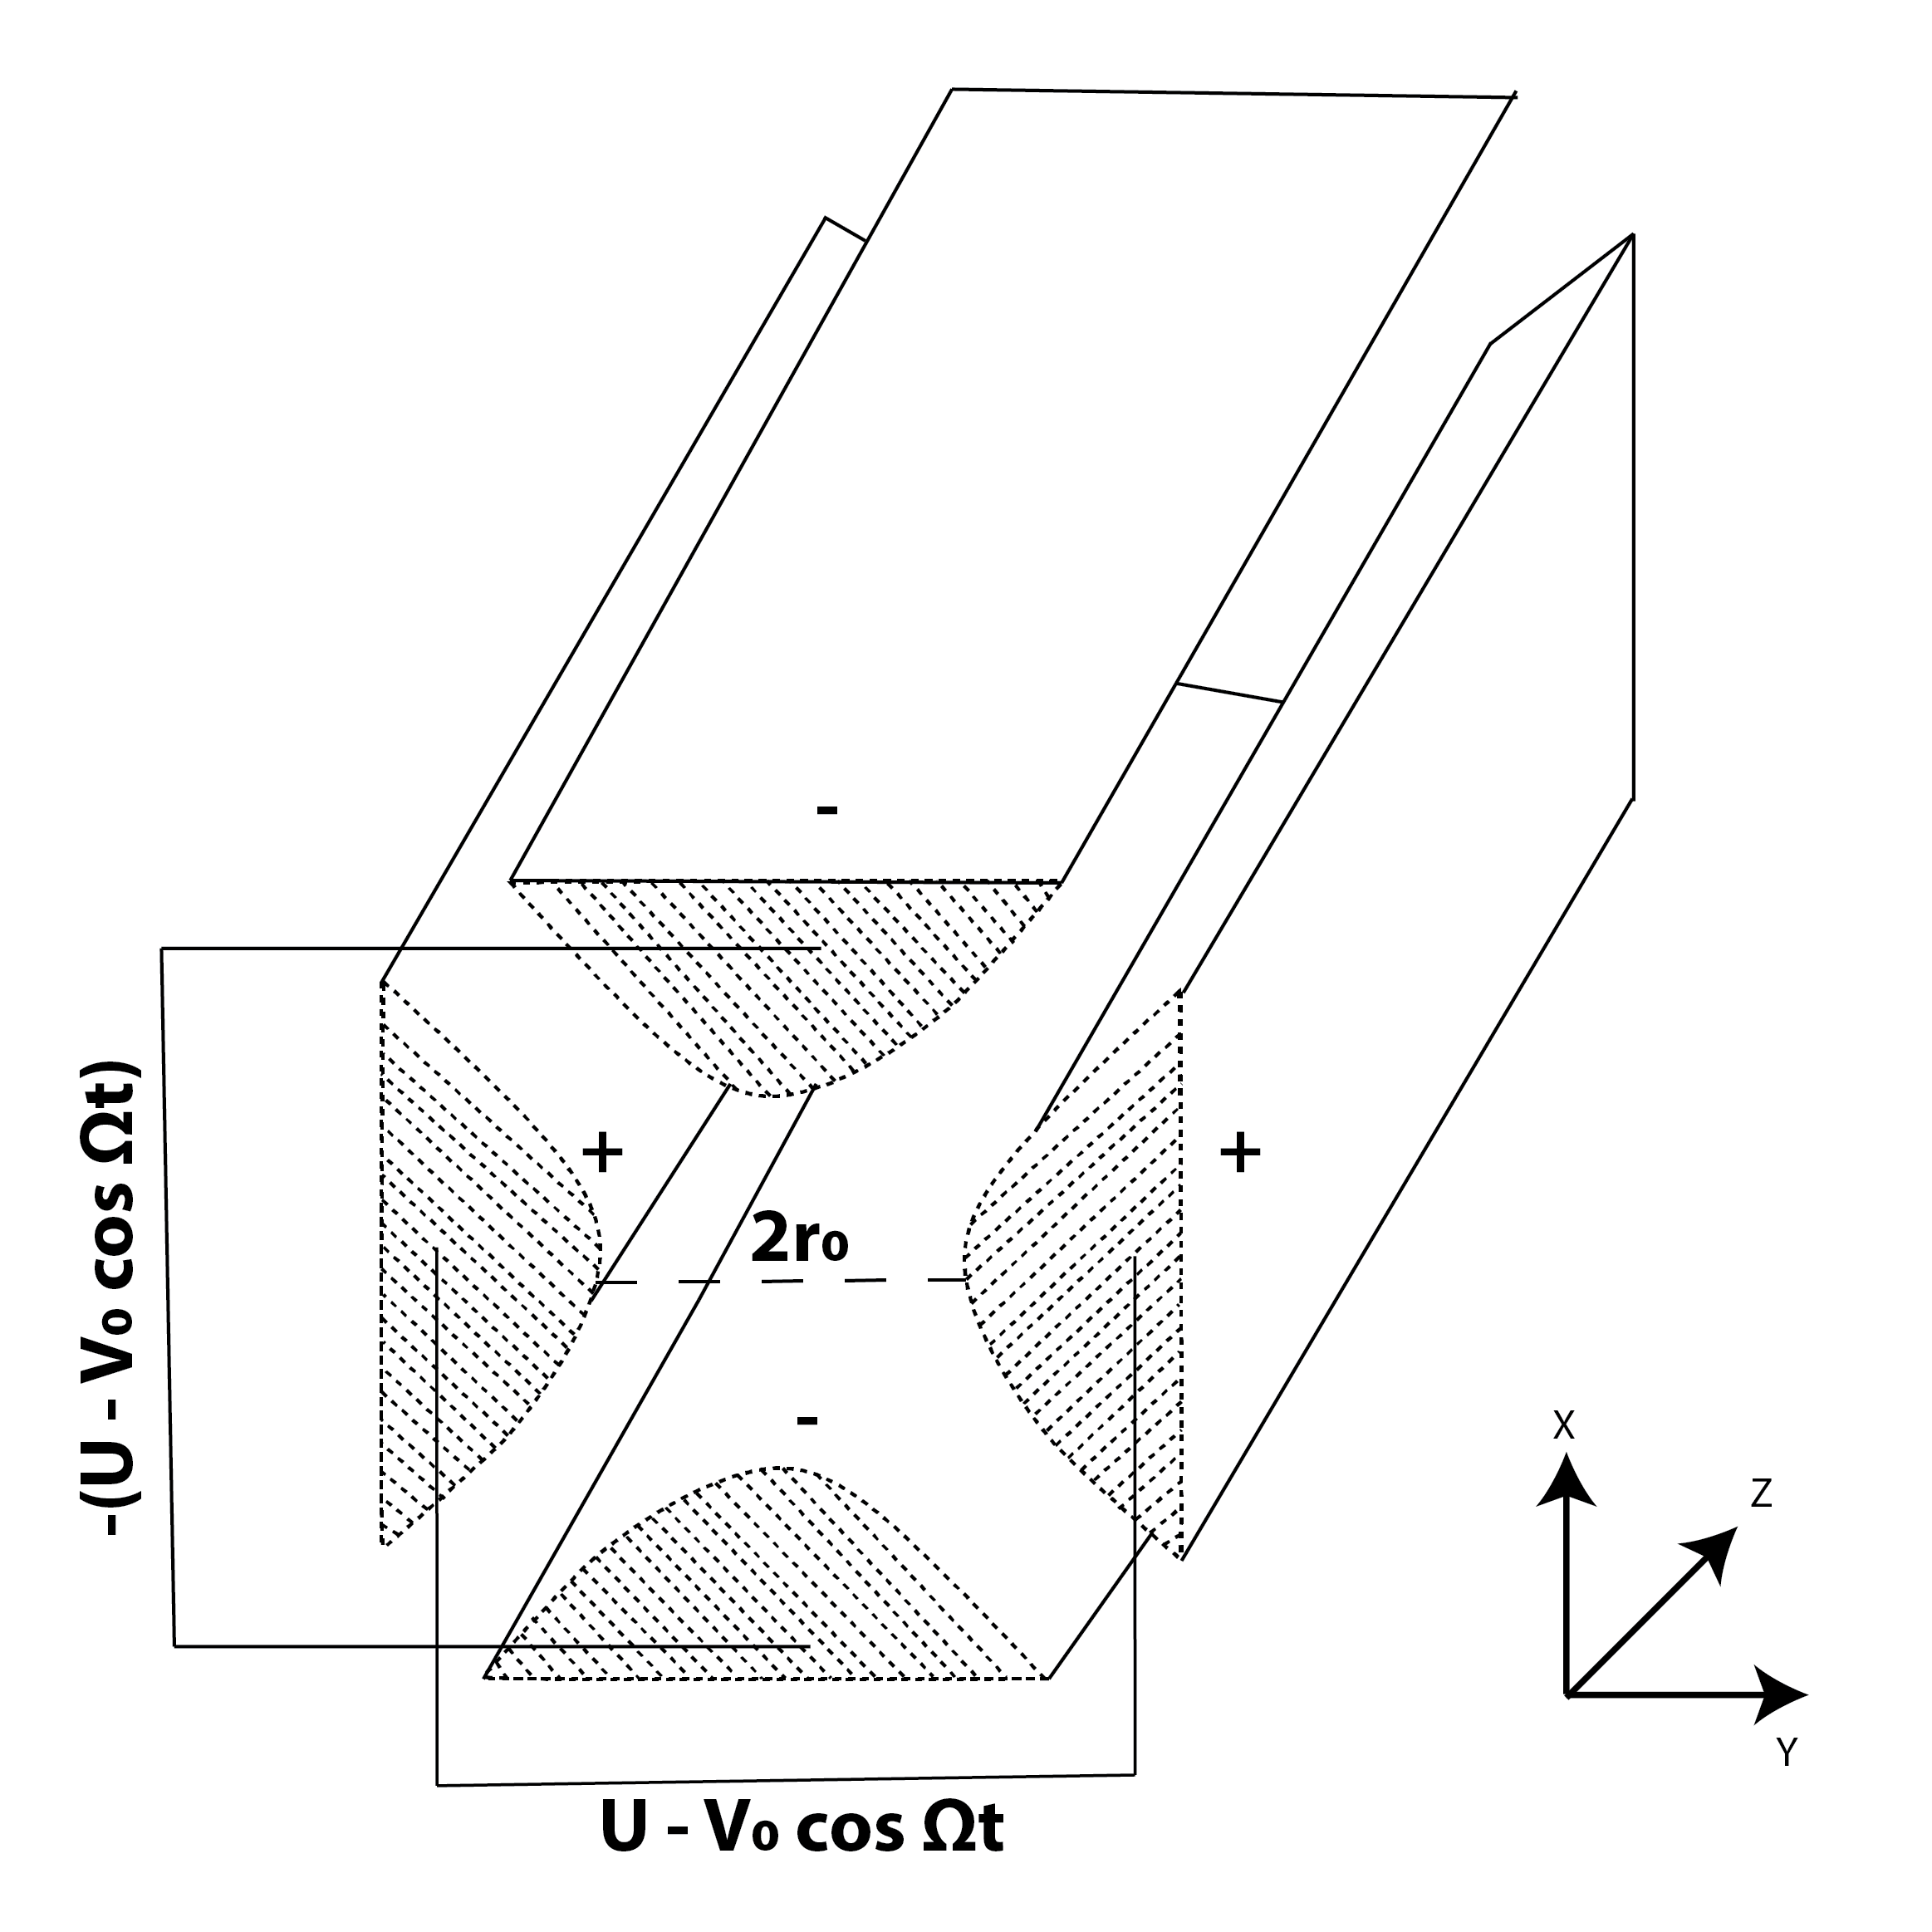
\includegraphics[width=0.5\textwidth]{figures/intro/trap/Quadrupole.png}
    \caption{Schematic diagram of a quadrupole mass filter. Ions enter and move along the z-axis as they oscillate in the x-y plane. The oscillation is regulated by applying DC (U) and radio frequency (RF) (V) potentials to each set of rods. Only ions with stable paths at the chosen U and V values will pass through the quadrupole mass filter.}
    \label{fig:quadrupole}
\end{figure}

\citet{paul_ionenka_1955} had developed the most basic electric field geometry known as the Paul or quadrupole ion trap. He also developed the quadrupole mass filter technique \cite{paul_elektrische_1955} (see Figure \ref{fig:quadrupole}). Using the combination of mass filter and ion trap, one can isolate and trap desired molecular ions with a specific mass-over-charge ratio ($m/z$). As a result, molecular spectroscopy in ions trap is routinely employed using action spectroscopic techniques \cite{SA2019, Roithovareview, Asvany2021}, as discussed in more detail in Section \ref{sec:action-spectroscopy}.

The trapped ions are usually cryogenically cooled to allow low temperatures experiments. Ion spectroscopic techniques typically employ collisional cooling with neutral buffer gas \cite{dehmelt_radiofrequency_1968, wester_radiofrequency_2009}. In the next section, we shall discuss the advantage of using a higher-multipole order ion trap, the 22-pole ion trap developed by \citet{gerlich_ion-neutral_1995}, and further improved by Asvany and Schlemmer \cite{asvany_note_2010} for low-temperature experiments under interstellar conditions.

\subsection{22-pole cryogenic ion trap}
\label{subsec:22-pole}

As discussed in Section \ref{subsec:intro:optical}, since the 1950s, ion chemistry under interstellar medium conditions has gained interest in exploring ion-molecule reactions at low temperatures and low-density \cite{smith_ion_1992, gerlich_experimental_1992}. Cryogenic ion trap experiments are commonly used to investigate laboratory ion-molecule reactions relevant to astrochemistry, and many astronomical objects have temperatures as low as 6 K \cite{harju_detection_2008}. However, in quadrupole traps, it is difficult to achieve low temperatures (kinetic and internal ion temperature) below $<10$ K \cite{gerlich_inhomogeneous_1992}. Therefore, higher-order multipole traps with large field-free zones are required for low-temperature astrochemical experiments.\\

\begin{figure}
    \centering
    \Subfigure[0.45]{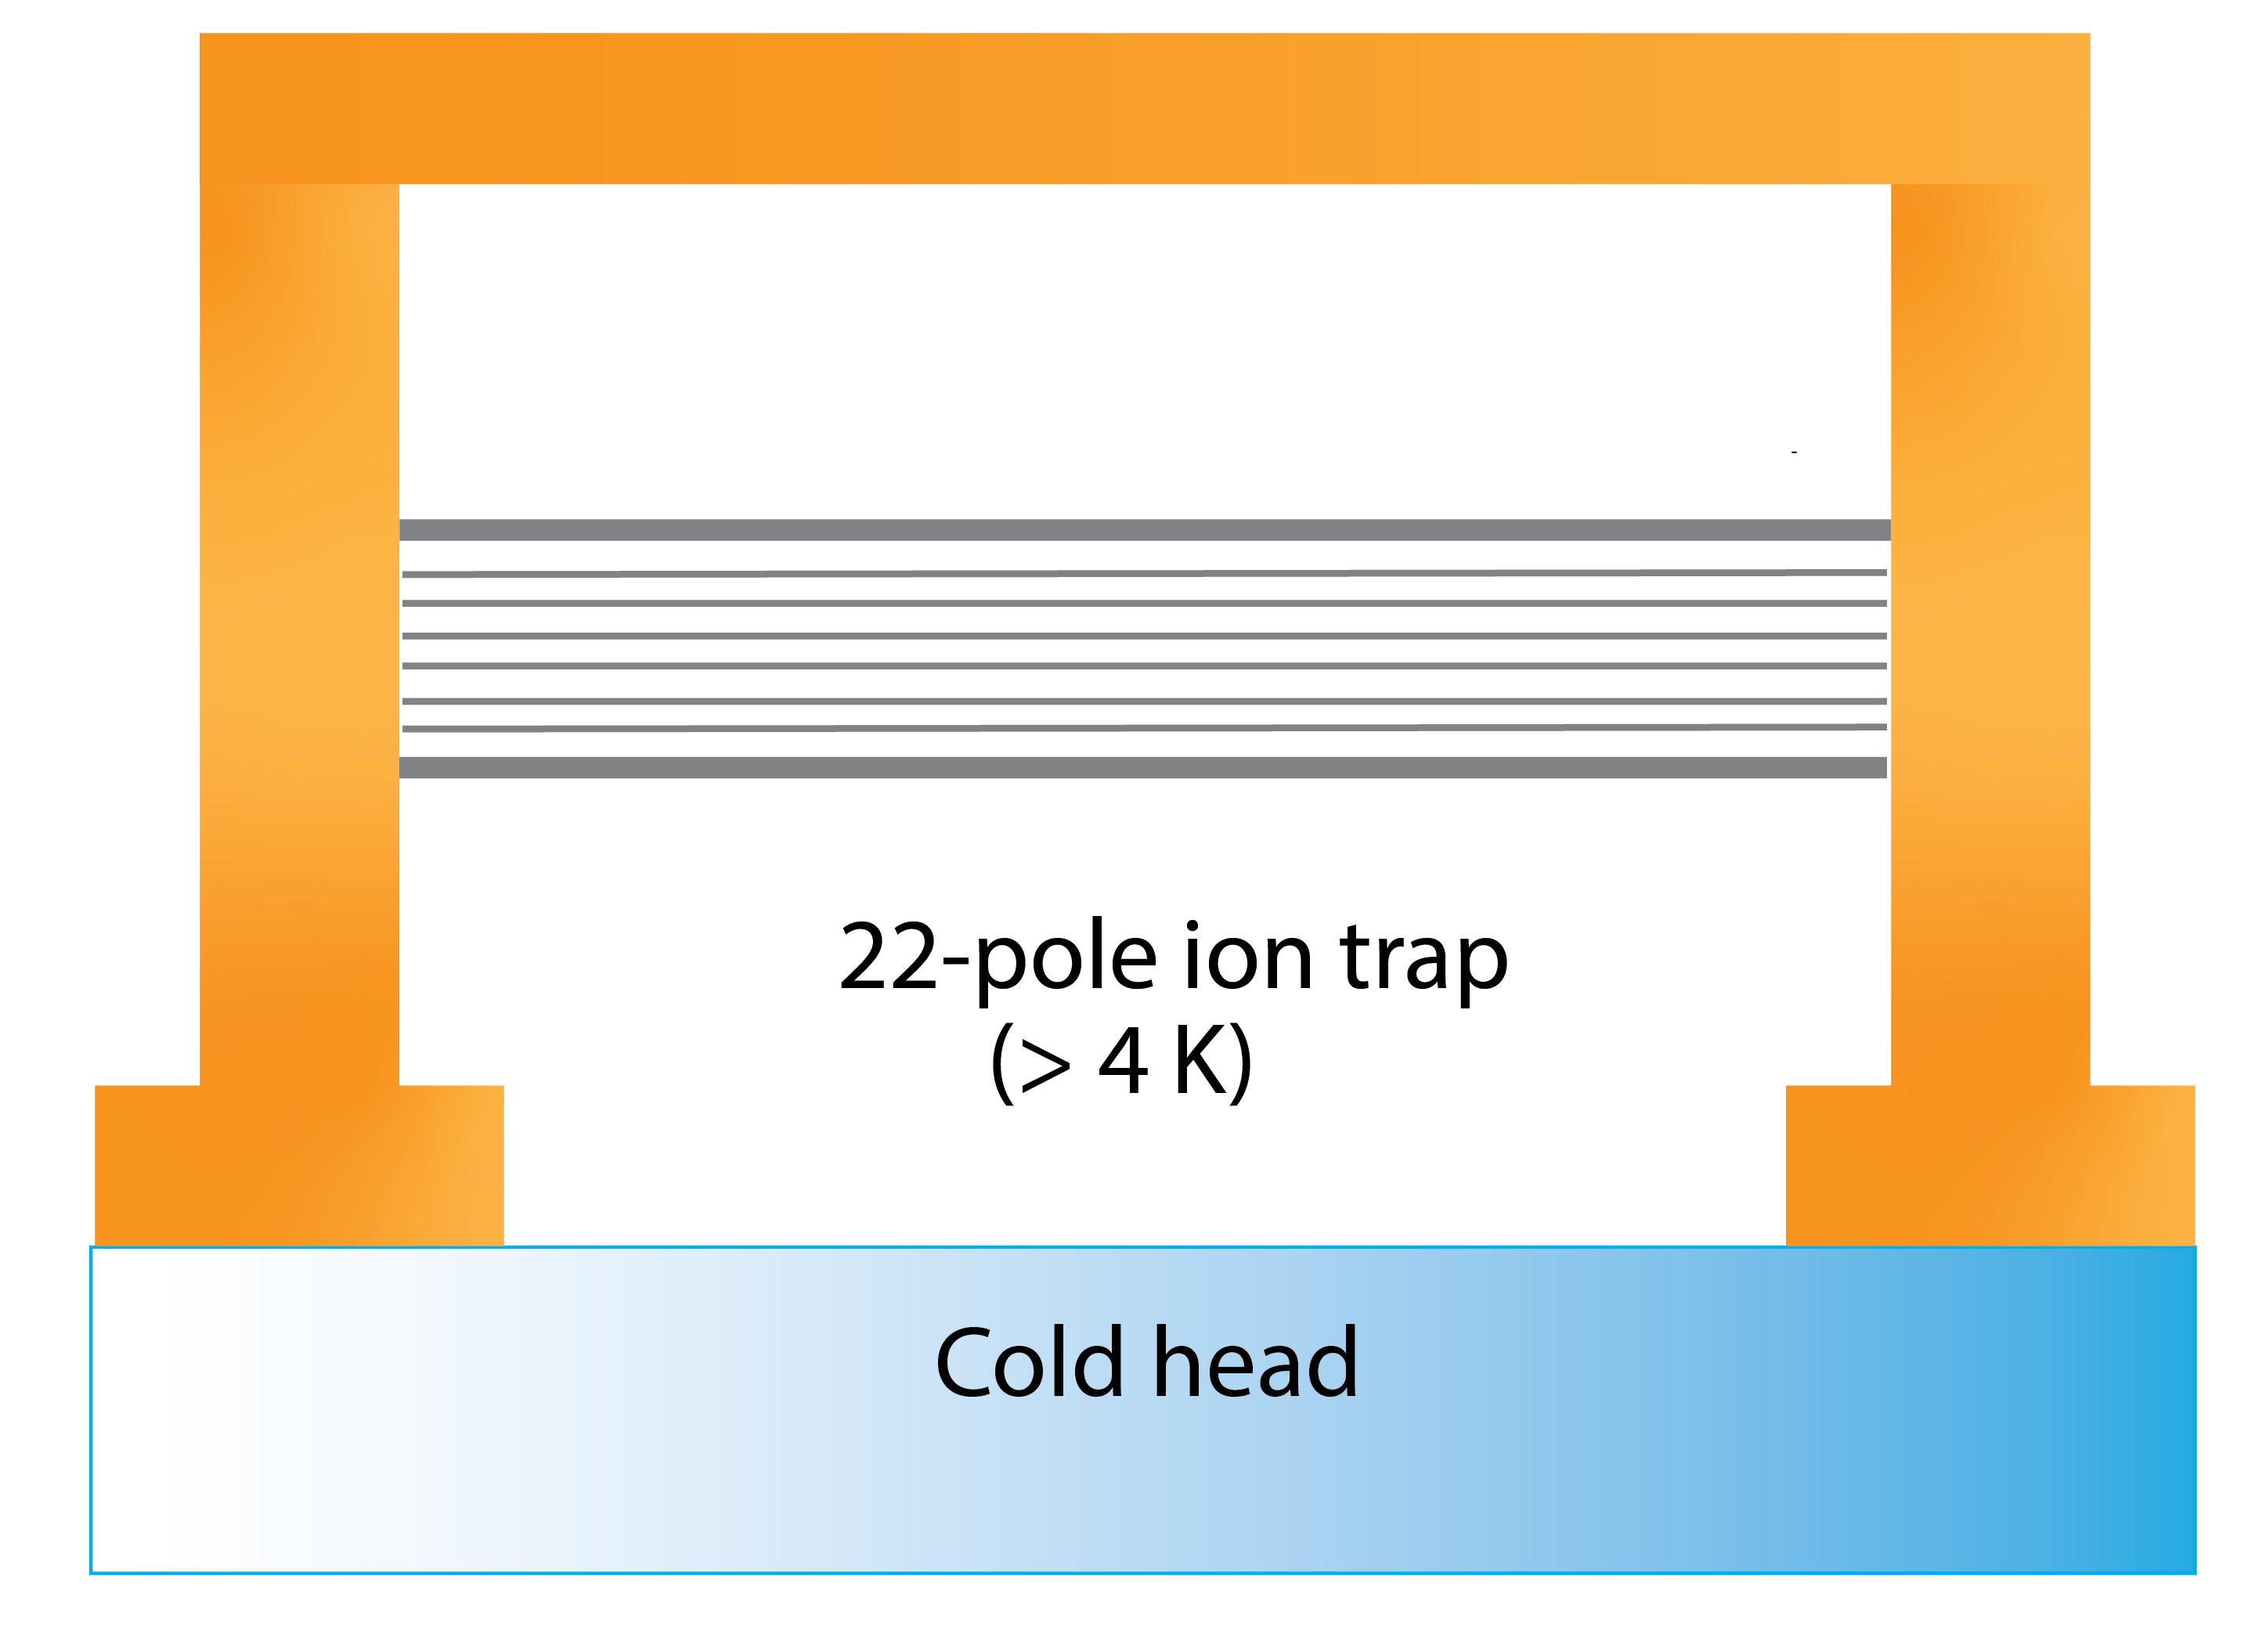
\includegraphics[width=1\textwidth]{figures/intro/trap/22-pole_ion - trap - coldhead.png}}{}{\label{fig:22-pole-iontrap-coldhead}}
    \hfill
    \Subfigure[0.5]{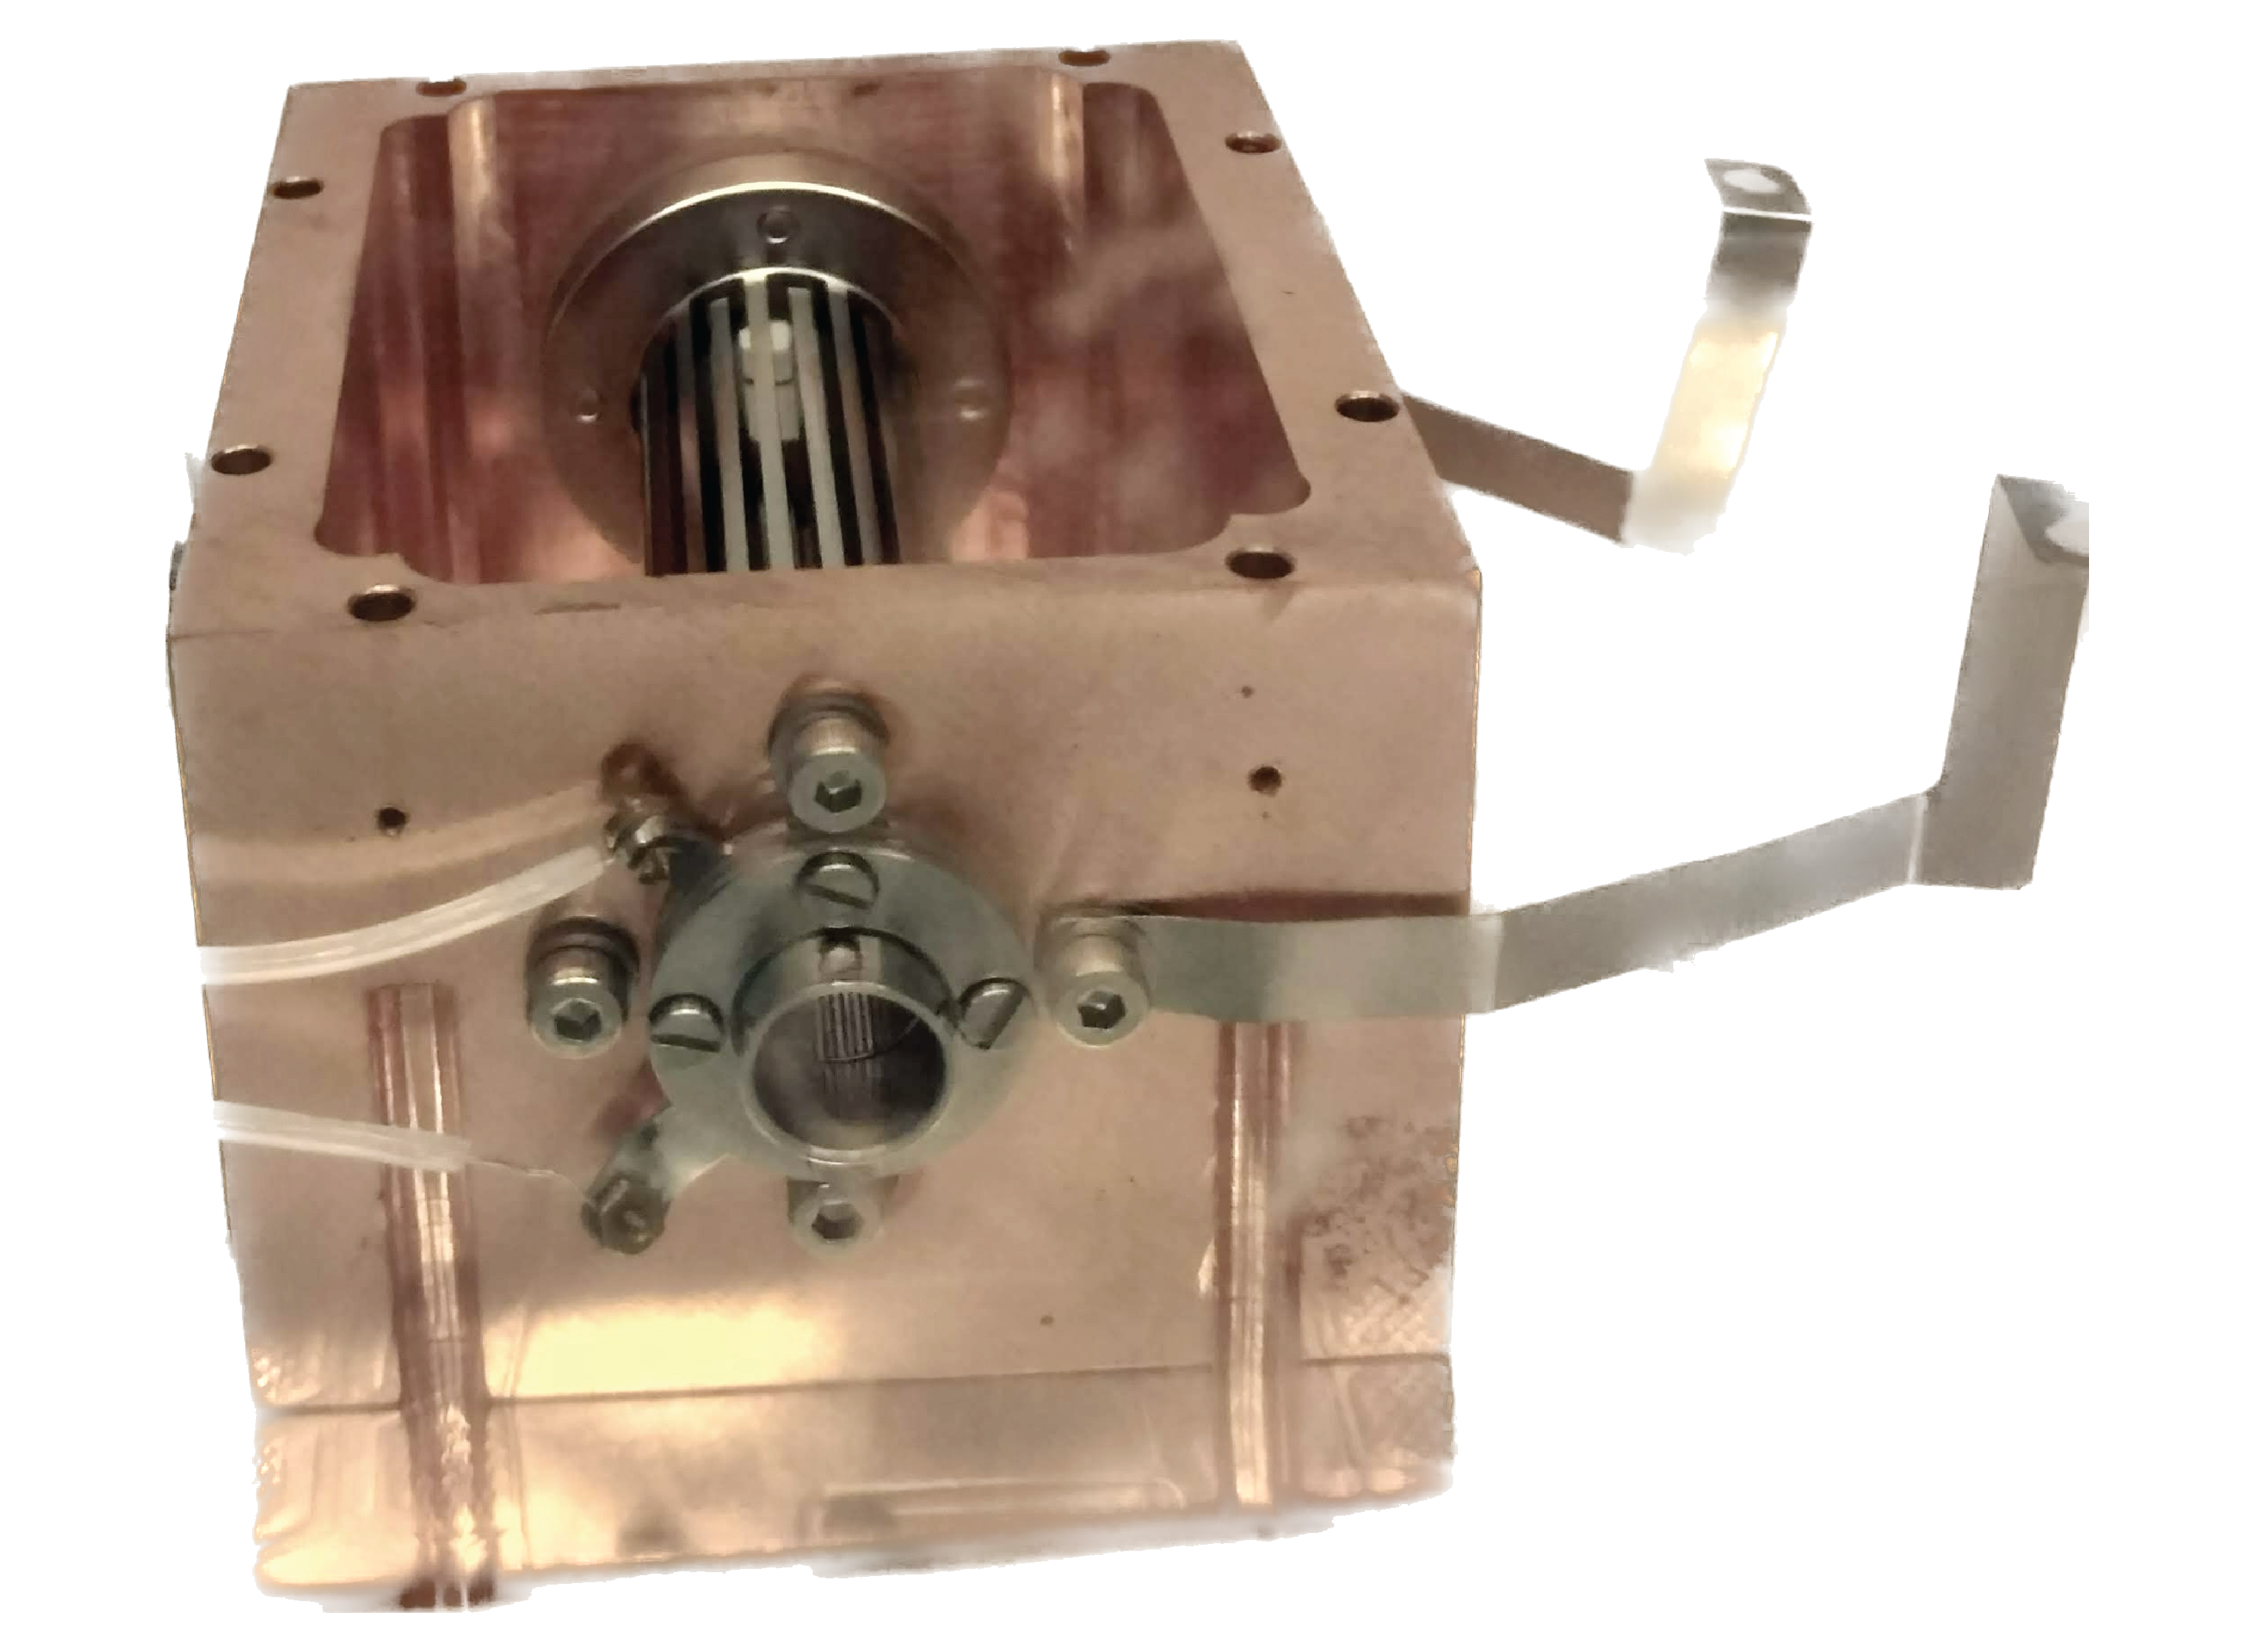
\includegraphics[width=1\textwidth]{figures/intro/trap/22PT.png}}{}{\label{fig:22PT-image}}
    
    \caption{(a) Schematic drawing of the 22-pole cryogenic ion trap (grey) in copper housing (orange) mounted onto cryogenic coldhead. (b) A photograph of the 22-pole ion trap mounted inside copper housing.}
    \label{fig:22PT}
\end{figure}

In a seminal review by \citet{gerlich_inhomogeneous_1992} titled \emph{Inhomogeneous rf fields: a versatile tool for the study of processes with slow ions}, the ideas of ion guiding and trapping using multipole fields have been described in great detail. Most notably, \citet{gerlich_ion-neutral_1995} also pioneered the development of the 22-pole ion trap (see Figure \ref{fig:22-pole-iontrap-coldhead}) for studies of ion-molecular reactions. The sensitivity and efficiency at low density and low temperature in 22-pole ion trap experiments is a major advantage over ion-molecule reaction studies at 300 K using other well-established techniques such as flowing afterglow (FA) \cite{fehsenfeld_thermalenergy_1967}, ion cyclotron resonance (ICR) ion traps \cite{kim_icr_1975}, and selected ion flow tube experiments (SIFT) \cite{smith_laboratory_1978}. With the development of the cryogenic 22-pole ion traps, significant advancements have occurred in studying low-temperature processes such as radiative association and three-body collisional processes in molecular complex formation \cite{gerlich_experimental_1992, paul_dynamics_1995, paul_deuteration_1996}.

The 22-pole cryogenic ion trap is also employed for high-resolution molecular spectroscopy of electronic \cite{chakrabarty_novel_2013, campbell_laboratory_2015}, vibrational \cite{asvany_understanding_2005} and rotational \cite{Brunken2017} transitions (see Section \ref{subsec:action:methods:vibrational} and \ref{subsec:action:methods:rotational}), including the first laboratory confirmation  of C$_{60}^+$ as the carrier of two DIBs by \citet{campbell_laboratory_2015}, using a 22-pole ion trap. It has gained even more popularity during the past two decades as a tool for researching ion-molecule interactions, and molecular ion spectroscopy  \cite{redwine_novel_2013, asvany_coltrap_2014, gunther_berlintrap_2017, jusko_felion_2019, rap_low-temperature_2022}.\\

In the next section, the action spectroscopic techniques developed in cryogenic ion traps for high-resolution molecular ion spectroscopy will be discussed.

\section{Action spectroscopy}
\label{sec:action-spectroscopy}

As discussed in Section \ref{sec:spectroscopy}, in contrast to absorption
spectroscopy, which detects the effect molecules have on light, action
spectroscopy measures effect of light on molecules. Ions are the optimum choice
for action spectroscopy methods because of their charge, which makes it easy to
guide, mass select and trap them efficiently. This section will focus only on
vibrational and rotational \qt{gas-phase action ion spectroscopy}.

\subsection{Vibrational action spectroscopy}
\label{subsec:action:methods:vibrational}

Photodissociation of isolated ions after light absorption (as long as the energy of the absorbed photons is higher than the bond dissociation threshold) is likely one of the most straightforward experimental techniques. So, most gas-phase action ion spectroscopy methods rely on the detection of charged products of dissociation or the loss of the parent ion signal after one or more photons are absorbed. In 1973, \citet{dunbar_photodissociation_1973} first investigated photodissociation in the visible spectral range. Soon after, \citet{okumura_vibrational_1985} studied photodissociation in the infrared region yielding the vibrational spectra.

In general, a single IR photon's absorption is insufficient to promote the breakdown of covalent bonds. However, several ways to circumvent this constraint are described in the following sections.

\subsubsection{Tagging photodissociation ion spectroscopy}
\label{subsec:action:methods:vibrational:IRPD}
The most straightforward technique to overcome the limitation is to utilise a loosely bound \qt{tag} to the molecular ion that detaches upon absorption of a single IR photon. The tags are chosen to have minimal effect on the structure of the ion core, i.e., they should be very weakly bound. Therefore, rare gas atoms such as He, Ne or Ar are preferred tagging agents.

The formed weakly bound complexes are dissociated as a result of resonance photon absorption as shown in Figure \ref{fig:IRPD} and the vibrational spectra are recorded as a function of IR frequency as shown in Figure \ref{fig:IRPD_spectrum}. This process is known as \qt{photo-dissociation} or \qt{pre-dissociation}. The very well-known technique using this approach for measuring vibrational transitions is called \qt{\textbf{I}nfra\textbf{R}ed \textbf{P}hoto-\textbf{D}issociation} (IRPD) spectroscopy.

\begin{figure}[!htb]
    \centering
    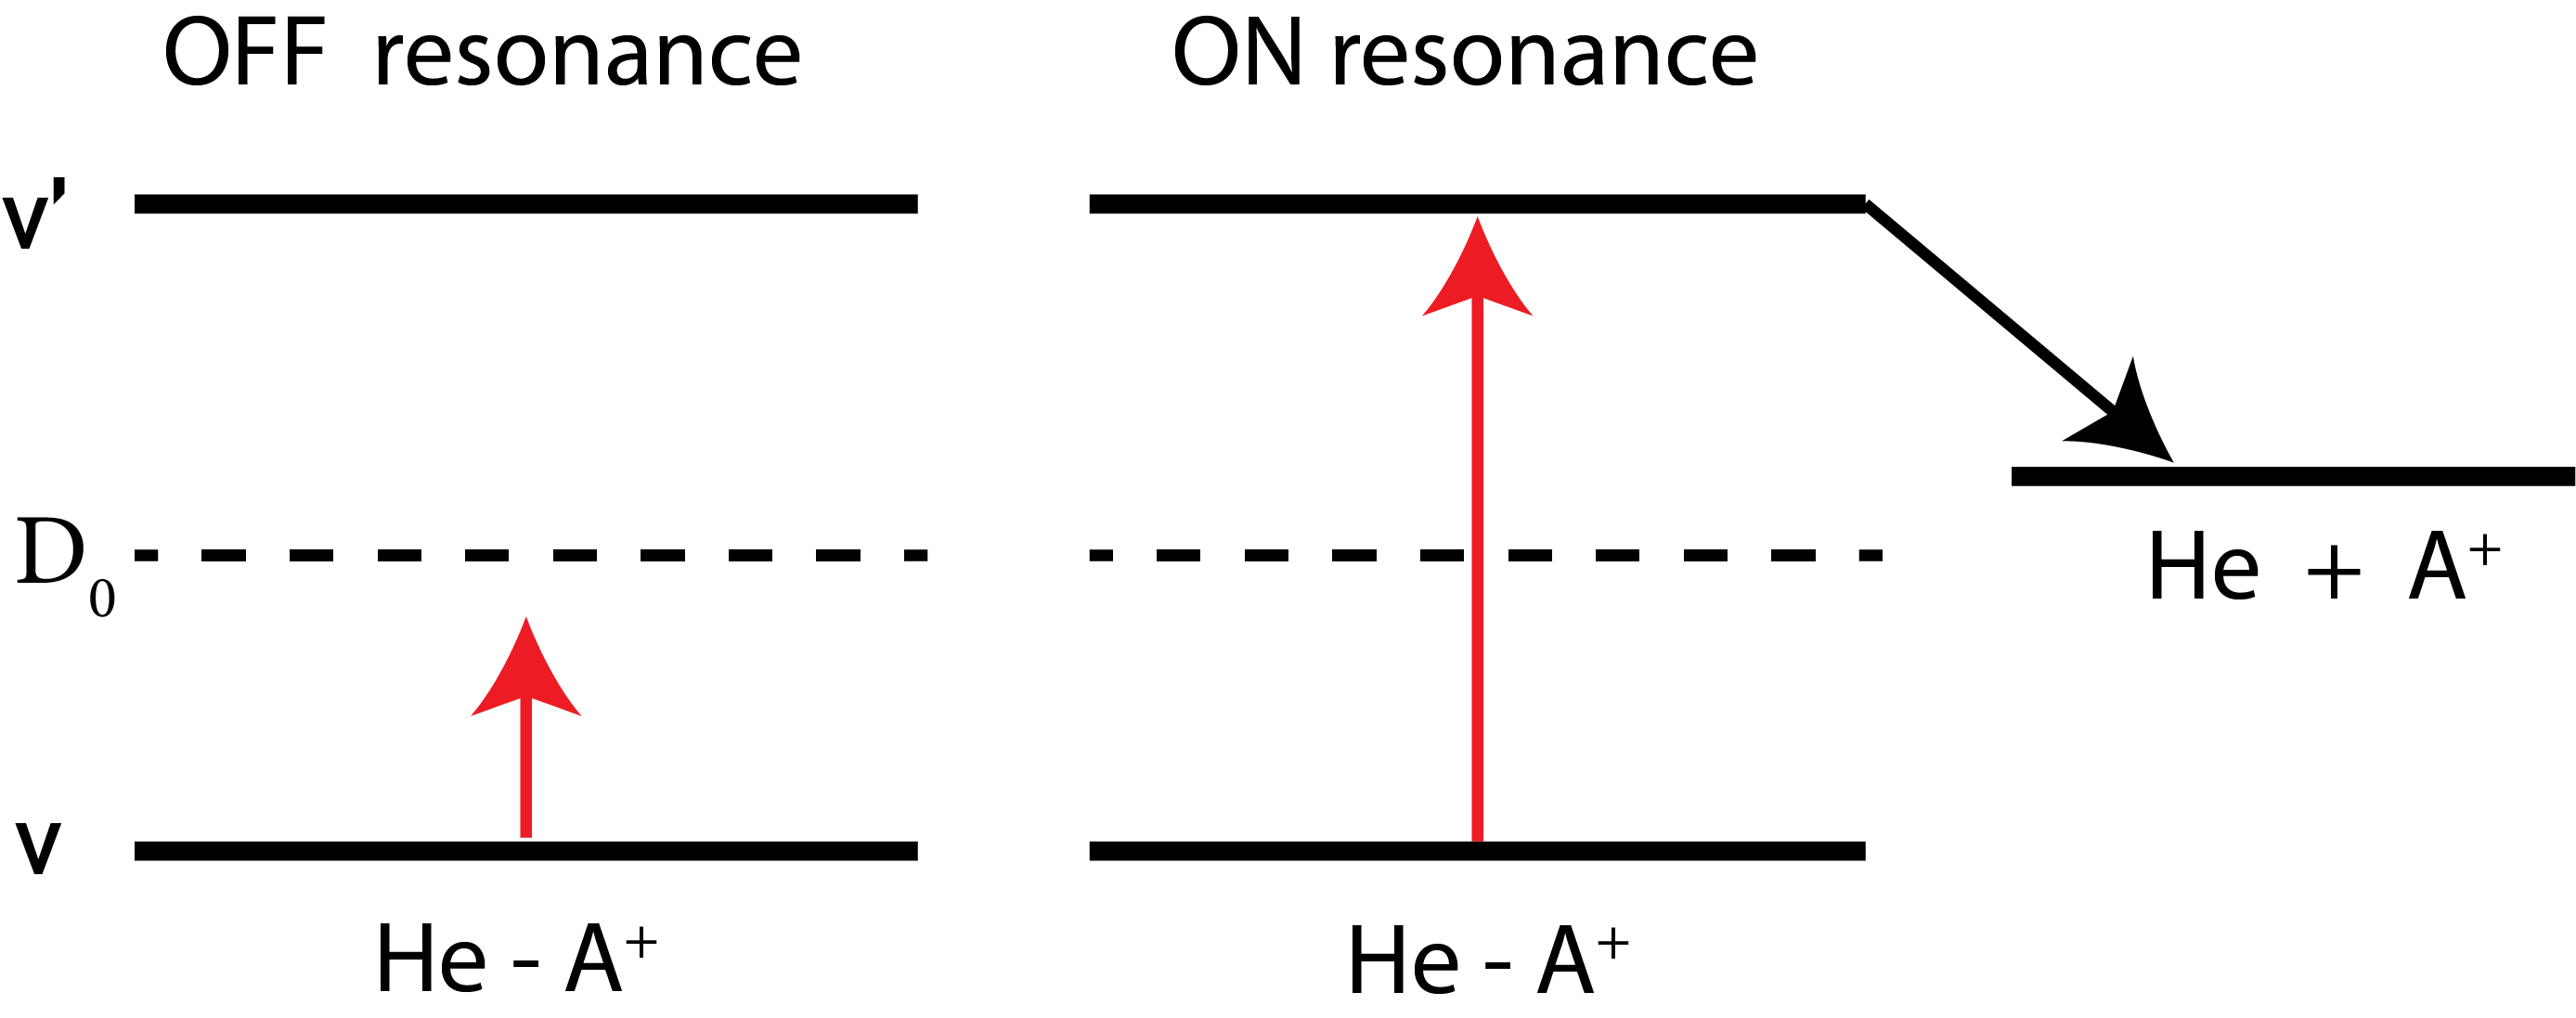
\includegraphics[width=0.9\textwidth]{figures/intro/IRPD.png}
    \caption{Schematic drawing of the IRPD method. He$-$A$^+$ represents the weakly bound helium complex of molecular ion A$^+$, and D$_0$ indicates the complex dissociation limit.}
    \label{fig:IRPD}
\end{figure}

\begin{figure}[!htb]
    \centering
    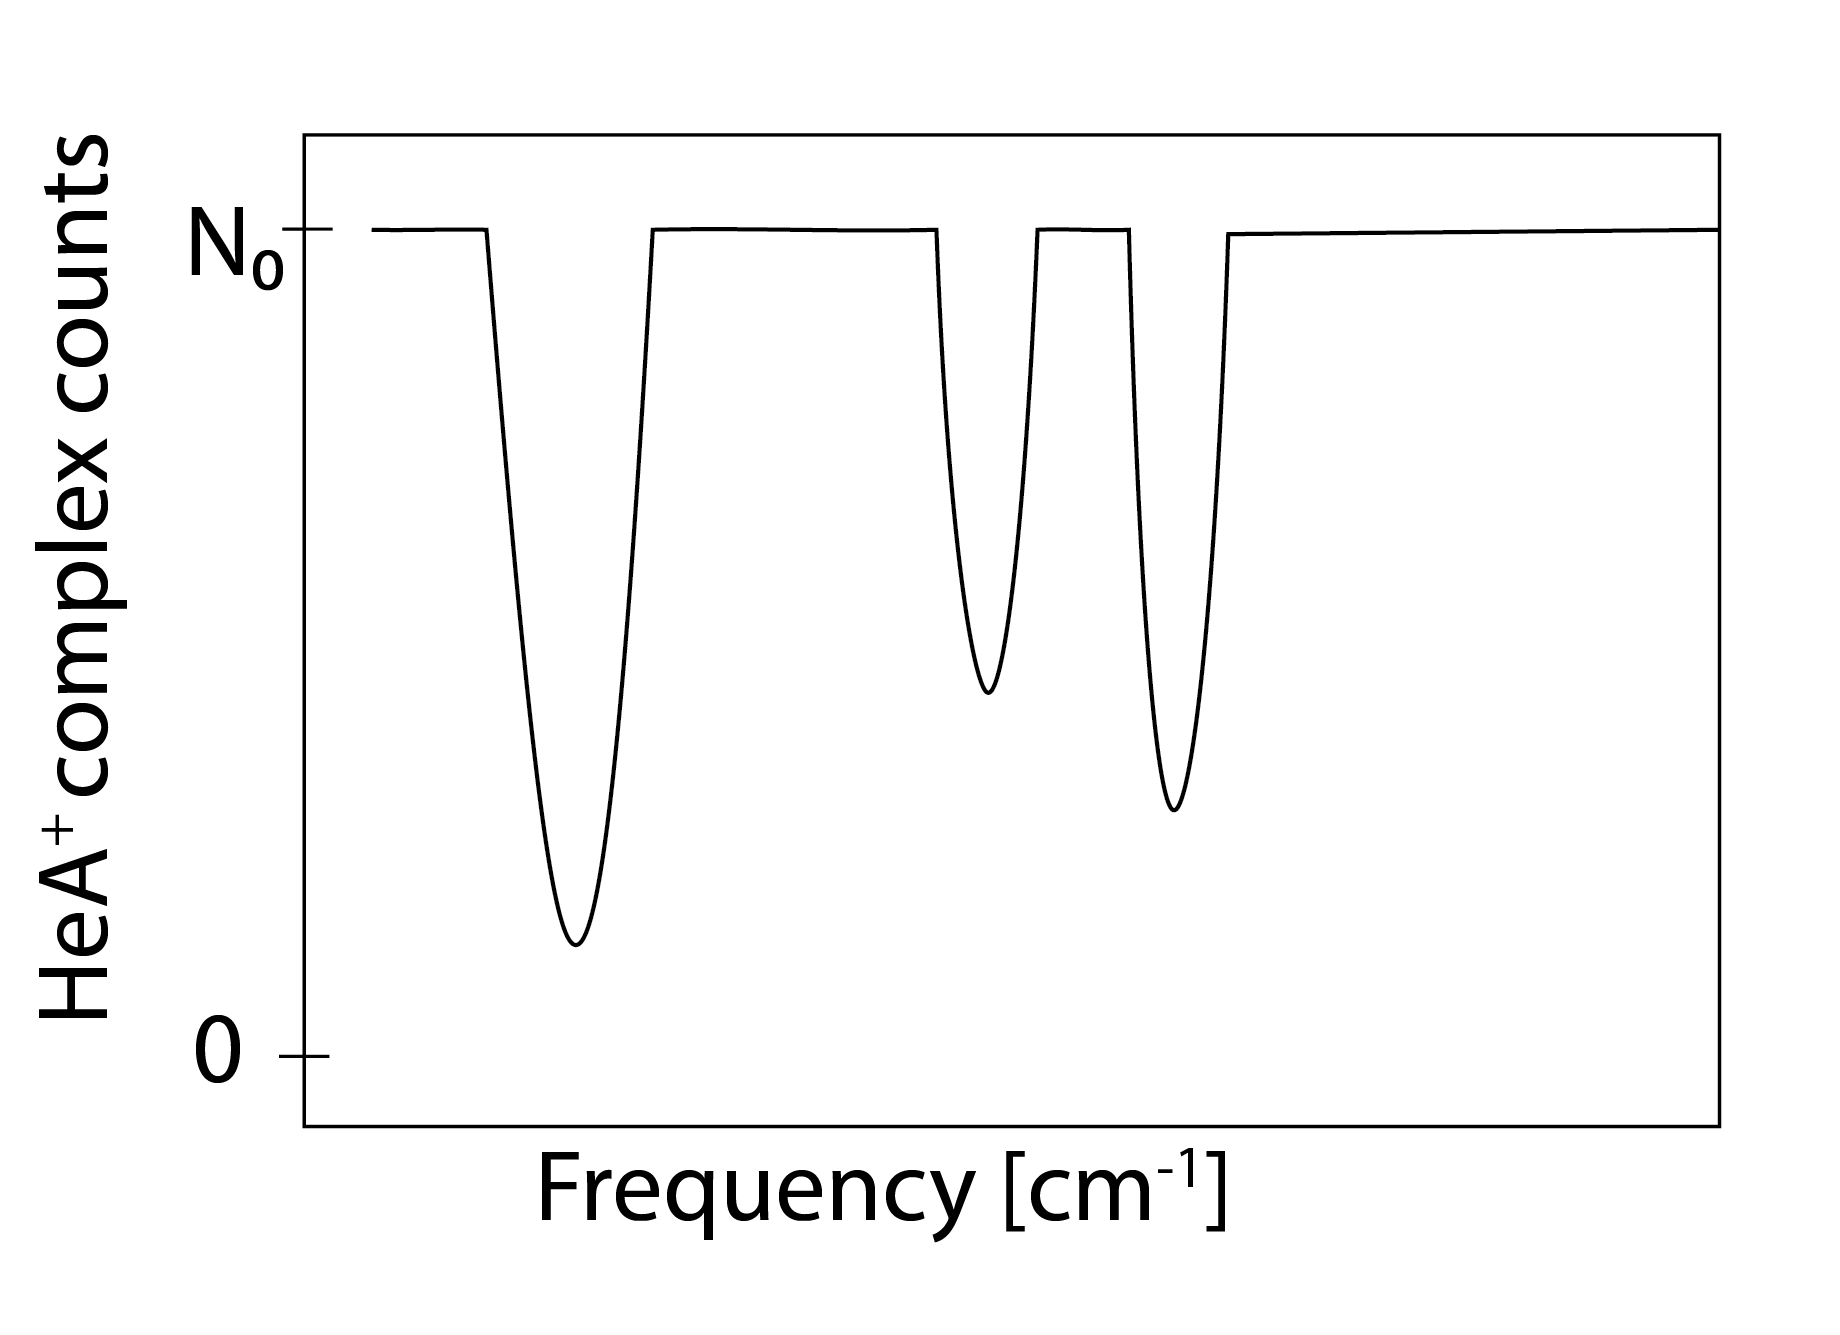
\includegraphics[scale=0.5]{figures/intro/IRPD_spectrum.png}
    \caption{Schematic IRPD spectrum measuring complex counts as a function of frequency. N$_0$ indicates the initial background counts, while the counts drop due to the dissociation of the complex at the resonance frequency.}
    \label{fig:IRPD_spectrum}
\end{figure}

Yuan T. Lee demonstrated the first  IRPD action spectroscopy technique  \cite{okumura_vibrational_1985} for hydrogen cluster ion, which several groups further developed \cite{bieske_spectroscopic_1993, duncan_infrared_2003, lisy_infrared_2006} using molecular beam experiments. However, in the molecular ion beam, the small interaction time between the ion and tag and ion and photons ( $\sim \mu$s range, flight time of ions) is a disadvantage for efficient complex formation and dissociation, respectively.
% Also, the ion sources synthesising weakly bound complexes often lead to vibrational hot bands.

Cryogenic ion trap experiments overcome these restrictions \cite{asmis_mass-selected_2002, kohguchi_high-resolution_2018, jusko_felion_2019, topfer_spectroscopic_2020, dahlmann_predissociation_2022} by storing for longer duration ($\geq 1$s) and by using cryogenic cooling to relax the molecular ion to its vibrational and electronic ground state. The low temperatures in the ion trap ($> 4$ K) also result in a high tagging efficiency even for weakly bound complexes \cite{roithova_helium_2016, gerlich_infrared_2018}, which is an important factor since the tagging method is predicated on the notion that the binding of the tag does not significantly alter the structure of the original ion. Consequently, the spectra produced from tagging spectroscopy can be correlated with the structure of "bare" ions.\\

The IRPD technique is employed in this thesis to characterize vibrational transitions of the molecular ion. Section \ref{sec:methods:vibration} discusses the integration of this technique into our 22-pole cryogenic ion trap instrument (Section \ref{sec:felion}). The following sections discuss several other methods developed for vibrational action spectroscopy.

\subsubsection{IR multi-photon dissociation (IRMPD)}
\label{subsec:action:methods:vibrational:IRMPD}

As discussed above, the energy of a single infrared (IR) photon is insufficient to cause dissociation in the majority of untagged ions. However, numerous photons can be absorbed when employing high-power light sources. The combined sum of the absorbed energy thus overcomes the dissociation energy limit, as shown in Figure \ref{fig:IRMPD}.

In 1973, Isenor and coworkers \cite{isenor_co2_1973} were the first to notice this IRMPD effect when they exposed SiF$_4$ vapour to powerful CO$_2$ laser pulses. This study was quickly replicated in laboratories worldwide, and it was later shown that many different types of molecules could undergo infrared multiple-photon dissociation or isomerization \cite{wight_infrared_1981, gaumann_infrared_1990, peiris_infrared_1993}. However, it was not until the 1990's that widely tunable free electron IR laser sources with adequate pulse energies became available, launching a new infrared ion spectroscopy area. \citet{oomens_gas-phase_2000} and \citet{lemaire_gas_2002} demonstrated the potential of a widely tunable infrared free-electron laser (FEL) in the study of the IR spectroscopy of mass-selected ions in an ion trap. 

\begin{figure}[!htb]
    \centering
    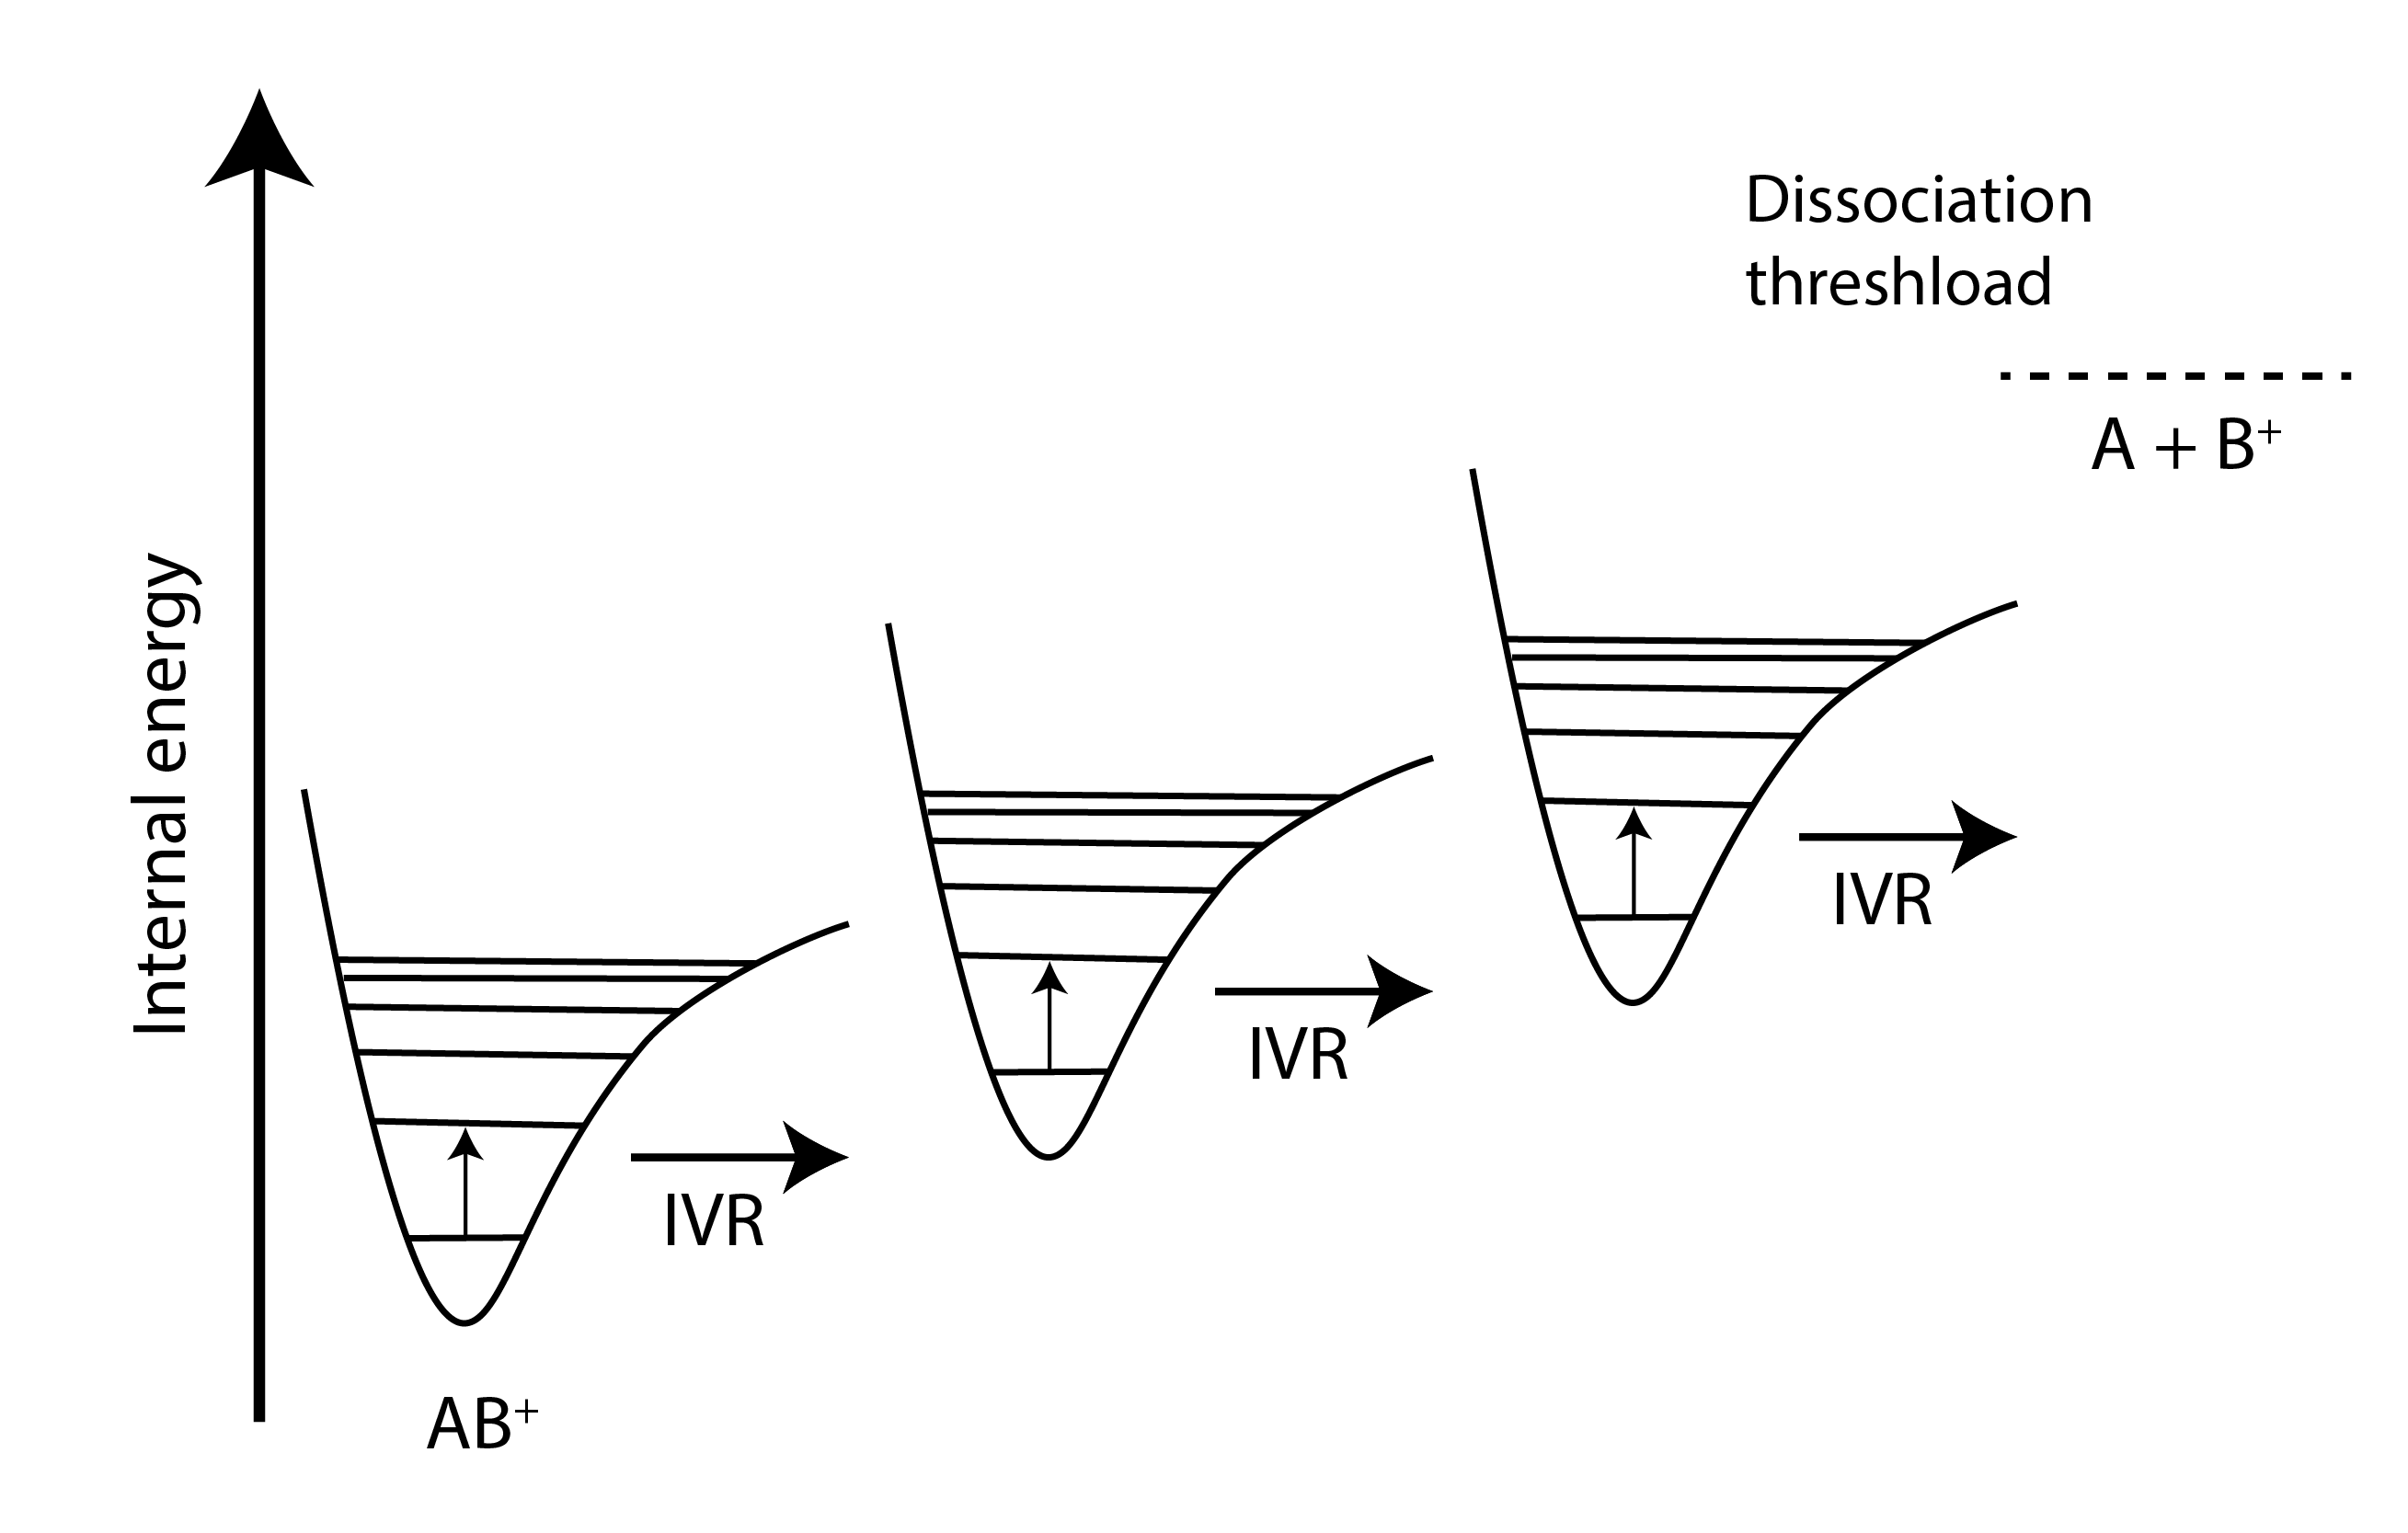
\includegraphics[scale=0.5]{figures/intro/IRMPD_IVR.png}
    \caption{Schematic drawing of the Infrared multi-photon dissociation (IRMPD) spectroscopy. AB$^+$ represents molecular ion consisting of A and B chemical fragments. Figure adapted from \cite{cpolfer_infrared_2011}.}
    \label{fig:IRMPD}
\end{figure}

Extensive experimental and theoretical research investigated the fundamentals of IR multiple-photon excitation in polyatomic molecules \cite{black_collisionless_1977, makarov_statistical_1998, oomens_gas-phase_2006, parneix_accurate_2013}. IRMPD is a low-energy fragmentation method that requires absorbing many photons of IR radiation before dissociation occurs. Vibrational potentials are inherently anharmonic, and absorption of tens to hundreds of photons occurs in a non-coherent manner. This effect is often referred to as the anharmonicity bottleneck \cite{steinfeld_molecules_1985}. Before the subsequent photon is absorbed, intramolecular vibrational redistribution (IVR) swiftly spreads the energy stored in the excited vibrational coordinate over all other vibrational degrees of freedom. The molecule is slowly heated, and dissociation typically follows the lowest-energy fragmentation pathway. 

However, this poses a difficult challenge to investigate small molecular ions using IRMPD because the method requires a high density of vibrational states, which guarantees that there are always a lot of vibrational eigenstates such that the IVR is feasible. Therefore IRMPD is typically well-suited for larger molecular ions. In this thesis, only smaller molecular ions ($\leq 7$ atoms) are investigated; hence IRPD is employed, as mentioned in the previous section.
% The other major disadvantage of IRMPD over IRPD is the broadening and shifting of the bands due to anharmonicity.

\subsubsection{Laser induced reactions (LIR)}
\label{subsec:action:methods:vibrational:LIR}

LIR combines the benefits of trapping molecular ions in a cryogenic ion trap with the idea of using a chemical reaction to determine the ion's internal state. In the late 1990s, \citet{schlemmer_laser_1999} developed LIR for spectroscopy by measuring the vibronic N$_2^+$ (A $ ^2\Pi_u \leftarrow$ X $^2\Sigma_g$) spectrum by excitation with visible laser photons to overcome the endothermic energy of a charge-transfer (CT) reaction as shown in equation \ref{eq:LIR:CT}. Counting the laser-induced product ions as a function of laser frequency yields the spectroscopic signal (see Figure \ref{fig:action:methods:vibrational:LIR-full}).

\begin{align}
    \text{N}_2^+ + \text{Ar} \rightarrow \text{Ar}^+ + \text{N}_2 \label{eq:LIR:CT}\\
    \text{C}_2\text{H}_2^+ + \text{H}_2 \rightarrow \text{C}_2\text{H}_3^+ + \text{H} \label{eq:LIR:H2_abstraction}\\
    \text{CH}_5^+ + \text{CO}_2 \rightarrow \text{CH}_4 + \text{OCOH}^+  \label{eq:LIR:proton_transfer}
\end{align}

\begin{figure}[!htb]
    \centering
    \Subfigure{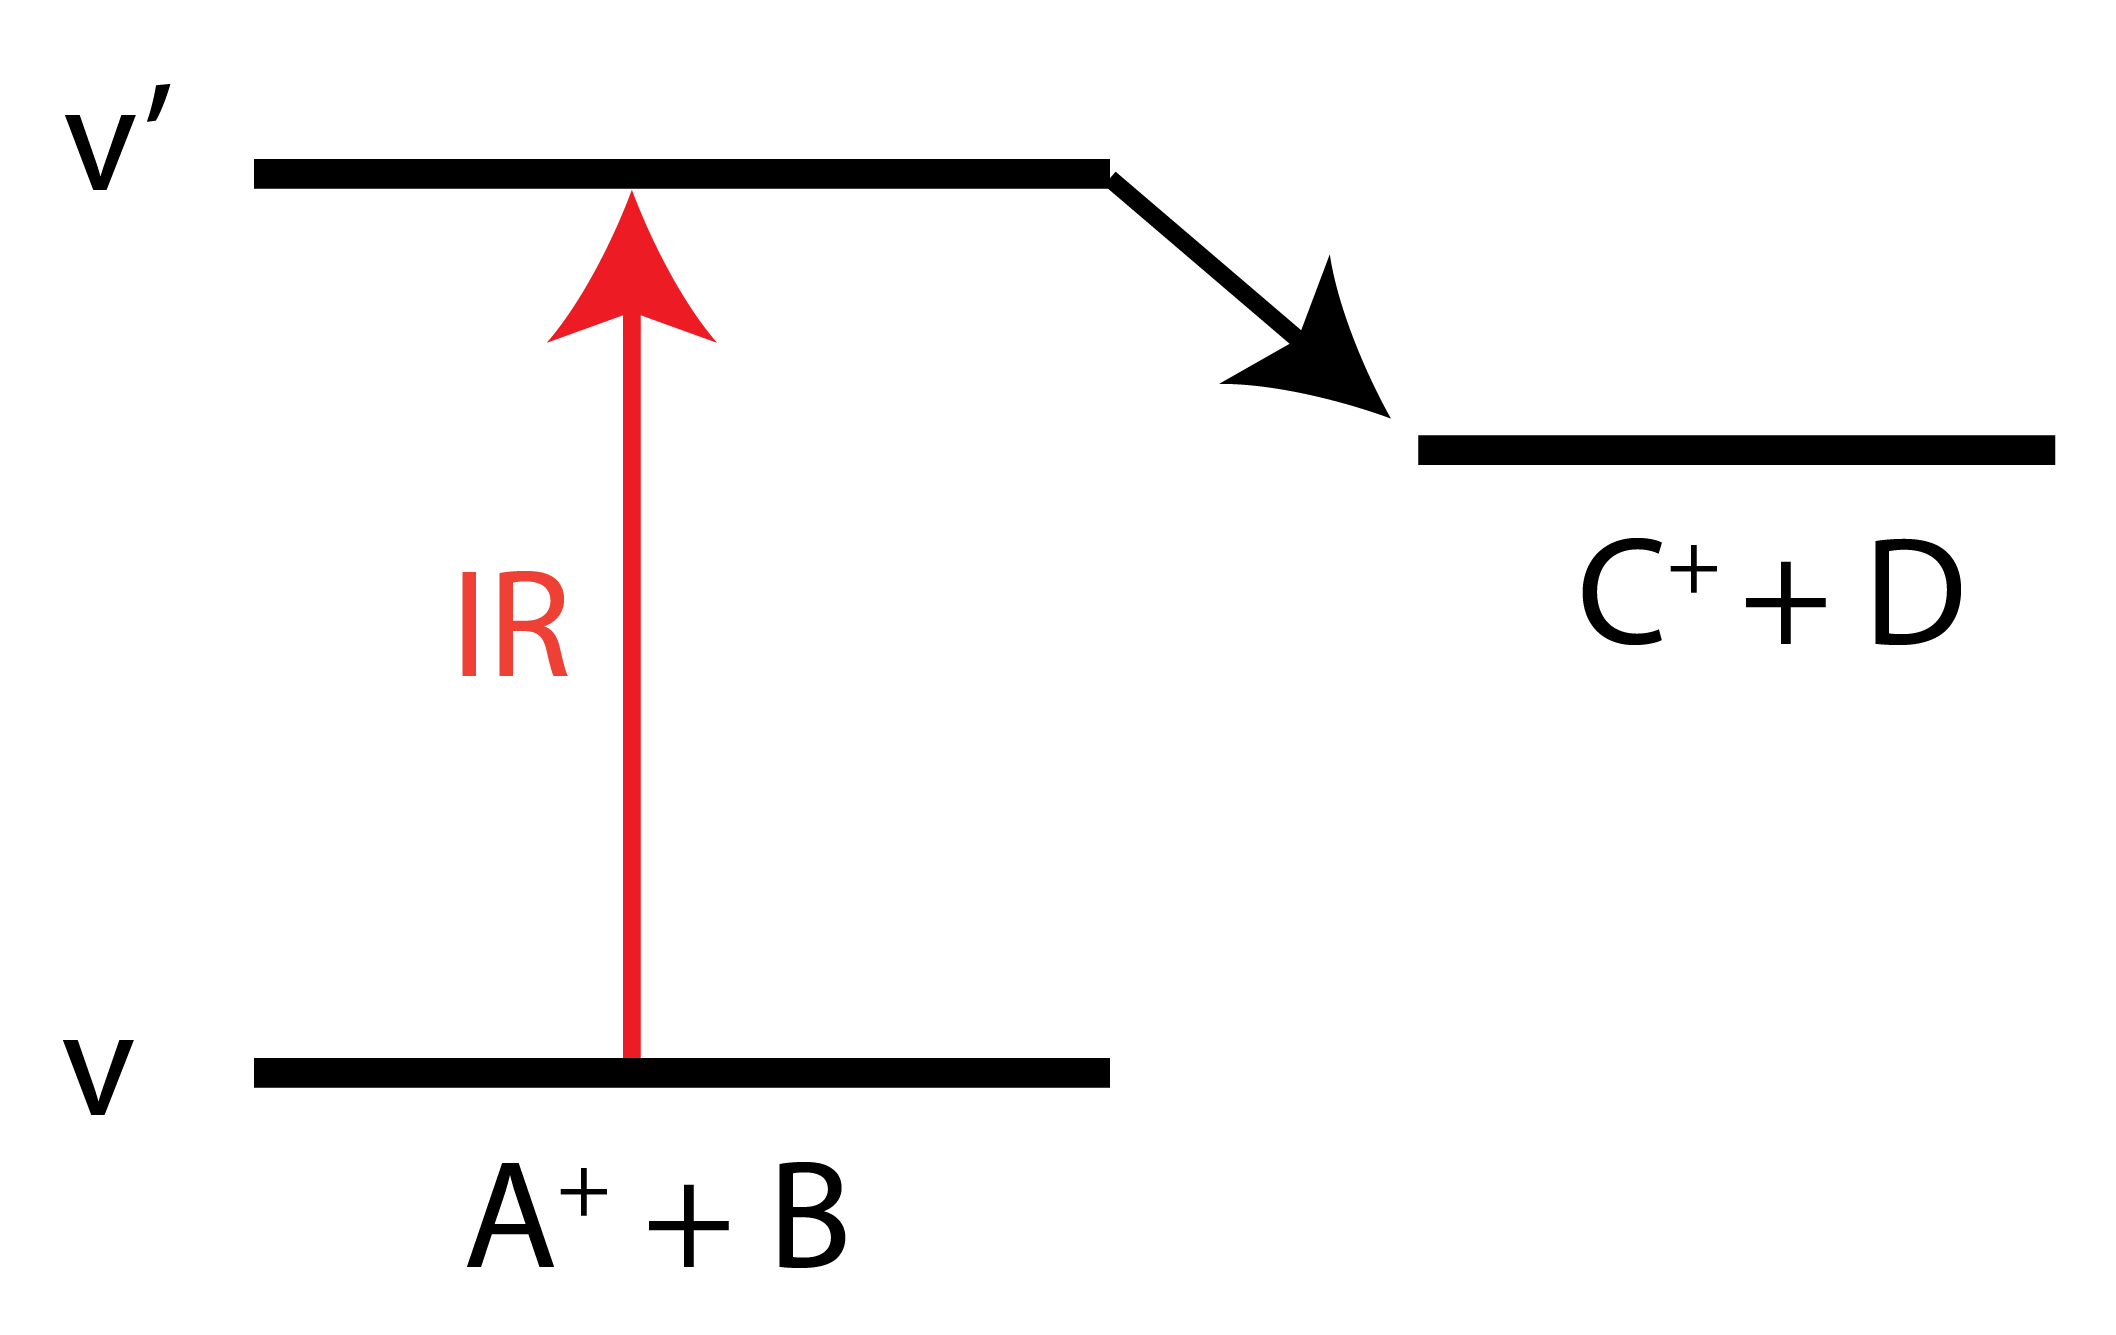
\includegraphics[width=1\textwidth]{figures/intro/LIR.png}}{}
    \hfill
    \Subfigure{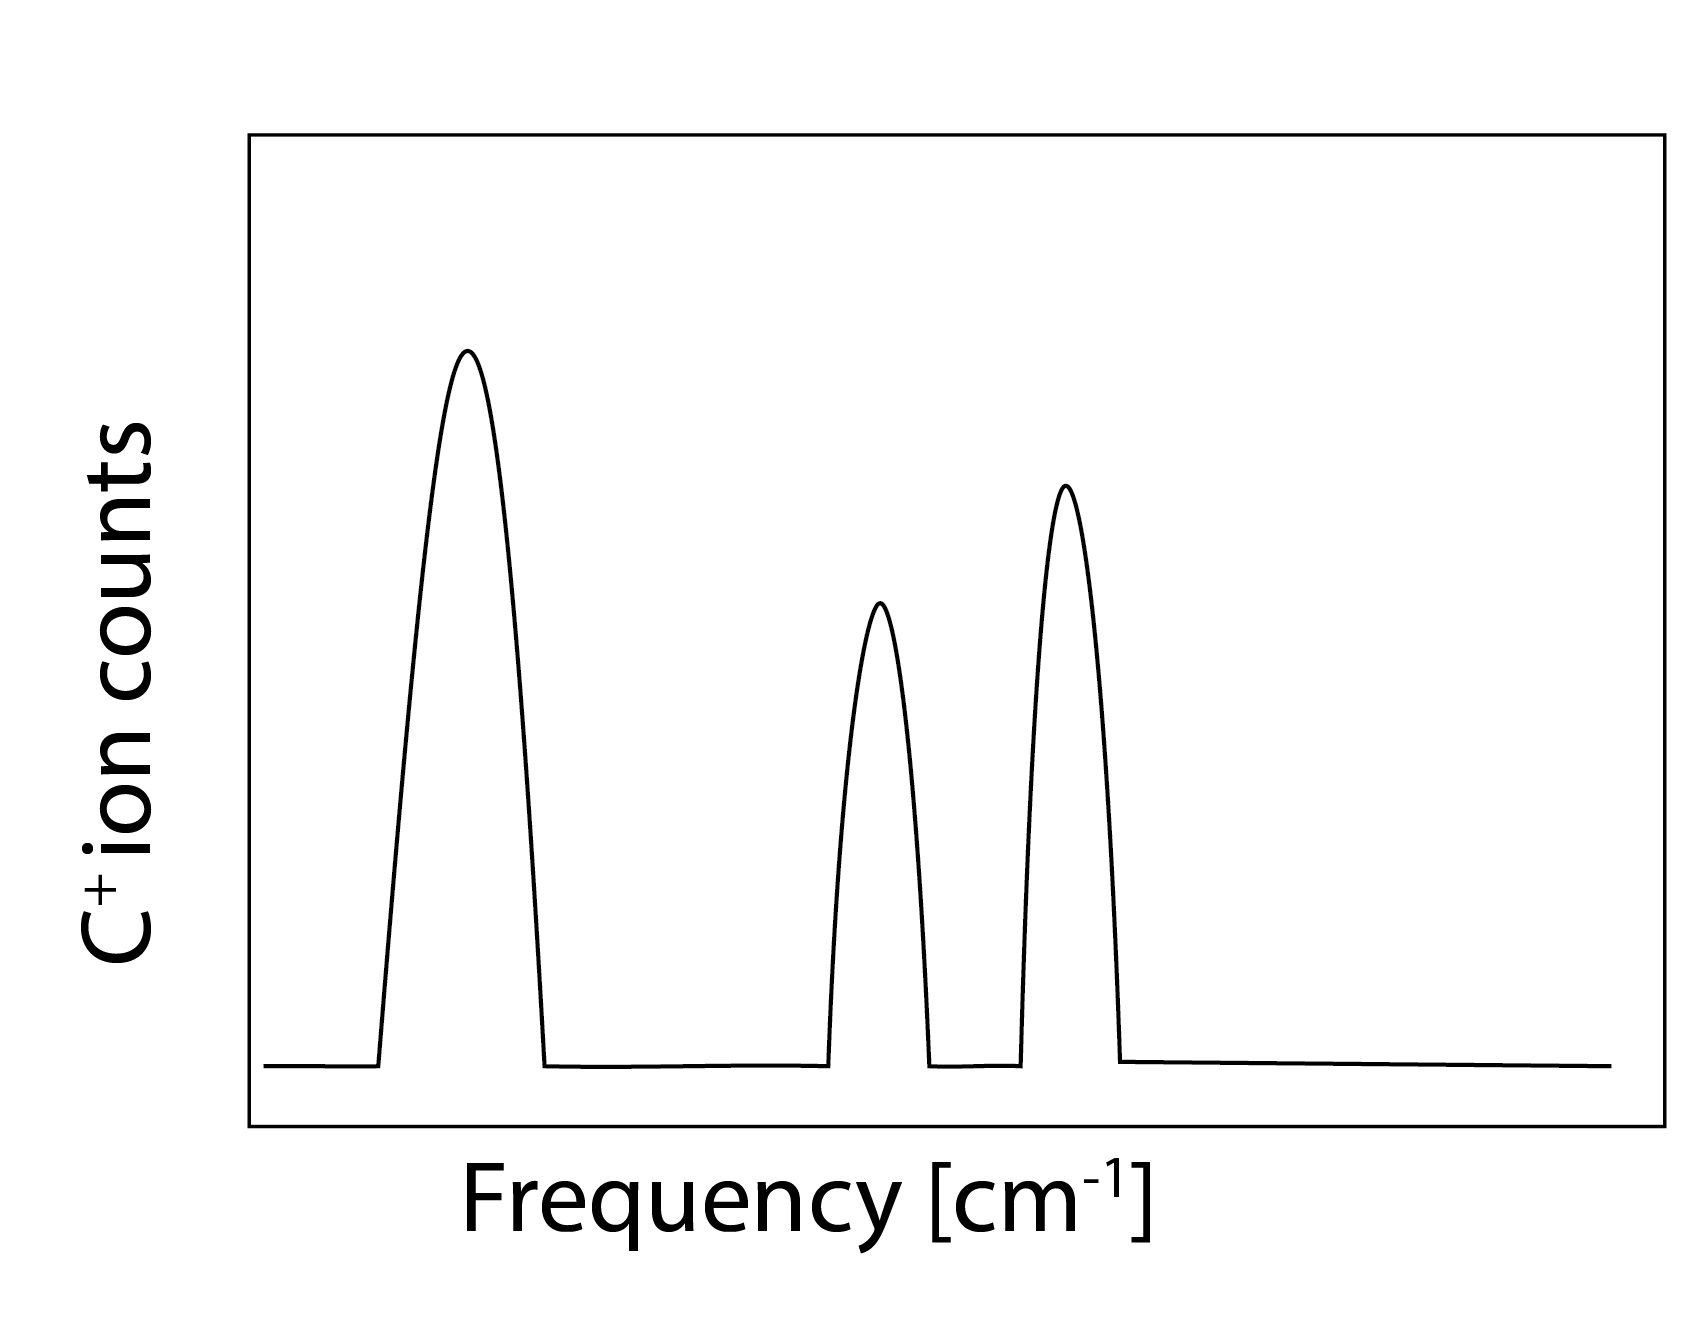
\includegraphics[width=1\textwidth]{figures/intro/LIR_spectrum.png}}{}
    \hfill
    \caption{Schematic description of (a) bimolecular reaction initiated by laser excitation suitable for LIR spectroscopy, (b) LIR signal as a function of frequency detected by monitoring the product counts.}
    \label{fig:action:methods:vibrational:LIR-full}
\end{figure}

Several endothermic reaction systems have been studied with the LIR method for bimolecular reactions, such as hydrogen abstraction and proton transfer (see Eq. \ref{eq:LIR:H2_abstraction} and  \ref{eq:LIR:proton_transfer}), to record vibrational transitions of reactant C$_2$H$_2^+$ \cite{schlemmer_laser_2002, asvany_experimental_2005, schlemmer_comparison_2005} and CH$_5^+$ \cite{asvany_understanding_2005}, respectively, by detecting the laser-induced products C$_2$H$_3^+$ and OCOH$_2^+$, respectively.

\subsubsection{Laser induced inhibition of He attachment (LIICG)}
\label{subsec:action:methods:vibrational:LIICG}

The requirement for an endothermic chemical reaction with a neutral reaction partner is a well-known limitation of the LIR method. Acquiring endothermic energy for chemical reactions is challenging, especially for highly reactive molecular ions. Also, the endothermicity cannot be too high since it needs to be overcome by the absorption of a single infrared photon. Another limitation is that since the cryogenic trap has very low temperatures, the reaction partner should not condense in the trap. These conditions limit the use of LIR.

LIICG takes advantage of the fact that the excitation of molecular ions can inhibit the ternary attachment of He atoms. Maier and Gerlich \cite{chakrabarty_novel_2013} pioneered this method by measuring the electronic transition of N$_2^+$ (A $ ^2\Pi_u \leftarrow$ X $^2\Sigma_g$) using a 22-pole cryogenic ion trap.

First vibrational LIICG was demonstrated for rovibrational transitions in the floppy CH$_5^+$ molecular ion by \citet{asvany_coltrap_2014} by forming CH$_5^+-$He complexes and observing an on-resonance decrease in the number of CH$_5^+-$He due to laser-induced inhibition of helium attaching to CH$_5^+$ (not via destruction of CH$_5^+-$He as in IRPD). The vibrational LIICG has been employed to record many other molecular ions such as O$_2$H$^+$ \cite{kohguchi_high-resolution_2018}, CH$^+$ \cite{domenech_first_2018}, H$_3^+$, H$_2$D$^+$ and D$_2$H$^+$ \cite{jusko_frequency_2016}, CD$_2$H$^+$ \cite{jusko_high-resolution_2017}, CH$_2$NH$_2^+$ \cite{Markus2019}, CN$^+$ \cite{domenech_high-resolution_2020}; HHe$_2^+$ and HHe$_3^+$ \cite{topfer_spectroscopic_2020}.

Interestingly, the ternary rate coefficient for He attachment can be affected by rotational excitation, even though rotational photons only carry a fraction of energy compared to vibrational photons. Section \ref{subsec:action:methods:rotational:ROSAA} describes how to use this phenomenon to our advantage to measure high-resolution molecular ions' rotational spectra.

% \subsubsection{Double resonance methods}
% \label{subsec:action:methods:vibrational:DR}

% Double resonance spectroscopy uses two spectroscopic light sources simultaneously, often at very different wavelengths. Because of availability of different combination of lasers, there are several methods developed to study conformer/isomer selective studies. Only few techniques invlolving IR and UV lasers are discussed here as an example in this section.\\

% The technique of infrared–ultraviolet (IR–UV) double resonance (DR) spectroscopy has proven to be an effective method for the measurement of the conformation-selective vibrational spectra of polyatomic molecules, ions, and their clusters. The method involves using an IR laser pulse to change the molecule's vibrational population, followed by a UV laser pulse to detect this variation.\\

% \textbf{IR-UV depletion spectroscopy: } In this double resonance spectroscopy, infrared (IR) and ultra-violet (UV) lasers are used. By locking the UV laser onto the specific electronic transition characteristic of the selected isomer. When an isomer absorbs an incoming IR photon, the ground vibrational state depopulates. This is measured as a decrease in the UV-induced photo-fragmentation signal, typically between 5\% and 50\% for IR laser pulses with an energy of 10 mJ \cite{stearns_conformation-specific_2007}. This depletion is recorded as a function of IR frequency to provide a isomer-specific IR spectrum. This technique can detect subtle differences between isomers.

% \textbf{IR-UV gain spectroscopy: }Ions are kept in their ground vibrational state by cooling them to cryogenic temperatures, which also minimizes the thermal broadening of the electronic transitions \cite{nagornova_exploring_2013}. Any isomer that absorbs an IR photon causes internal heating, which causes broaden and redshift of the corresponding electronic spectrum. The infrared photodissociation spectra of ions are recorded using these changes in the electronic absorption. The UV laser wavelength is adjusted to the red of the cold ion's lowest energy electronic transition, which prevents dissociation. The spectrum is recorded as a function of IR frequency and on-resonance the spectral broadening caused by IR photon absorption increases the dissociation (signal gain).\\


\subsection{Rotational action spectroscopy}
\label{subsec:action:methods:rotational}

Action spectroscopy for measuring rotational transitions is very challenging
since the rotational transition energies are much lower than vibrational or
electronic energy (see Table \ref{tab:electromagnetic_spectrum}). While
vibrational and electronic action spectroscopic methods have been available for
trapped ions and ionic clusters since the 1980s, the first rotational action
spectroscopic methods appeared only a decade ago from Schlemmer's group
\cite{Asvany2008}.

This section briefly summarises the detailed review by
\citet{Asvany2021} but focuses only on rotational action spectroscopic methods.
Figure \ref{fig:action:methods:rotational} shows the summary of rotational
action spectroscopic methods schematic diagrams.

\subsubsection{Rotational LIR}
\label{subsec:rotational-LIR}

Schlemmer and coworkers showed the first realization of pure rotational action
spectroscopy in a cryogenic trap using a direct-LIR method (as discussed in
Section \ref{subsec:action:methods:vibrational:LIR}) \cite{Asvany2008}. Using
this approach, they measured the lowest-lying rotational transitions of 
\emph{para-}H$_2$D$^+$ and \emph{ortho-}D$_2$H$^+$, two astronomically
important molecular ions that exhibit large rotational energy spacing (1.37 THz
and 1.48 THz for the ground state transitions, respectively). The on-resonance
laser-induced reactions of H$_2$D$^+$ and D$_2$H$^+$ held in a cold ion trap
increases the reactivity (producing H$_3^+$ and H$_2$D$^+$, respectively) with
a neutral H$_2$ reaction partner. Therefore the rotational transitions of the
investigated ions are reflected in the yield of the reaction products as shown
in Figure \ref{fig:action:methods:rotational:LIR}.

\subsubsection{Double resonance methods}
\label{subsec:action:methods:rotational:DR}

As discussed in Section \ref{subsec:action:methods:vibrational:LIICG} there are
limitations to the direct-LIR technique. Therefore further rotational action
spectroscopic techniques were later developed to generalise the scheme for a
wide range of molecular ions, such as using a double resonance approach. A
vibrational action spectroscopy scheme can be used to perform high-resolution
rotational spectroscopy by double resonance. In other words, if a molecule has
a vibrational action spectroscopy scheme with a rotational resolution, the
spectroscopy can easily be extended into the rotational domain by a double
resonance approach; the possibilities are as follows:

\textbf{\emph{via} LIR}: As shown in Figure \ref{fig:action:methods:rotational:DR_LIR}, this method uses a combination of infrared (IR) and Terahertz (THz) radiation to irradiate ions. The frequency of the IR photon is kept fixed on a rovibrational transition. The signal is monitored by counting the number of the product ions produced as a function of the THz frequency \cite{Gartner2013,jusko_two-photon_2014}. The signal can be depletion or gain depending on whether the IR is fixed at a rotational ground or excited state.

\textbf{\emph{via} predissociation:} Predissociation is another effective vibrational action spectroscopic technique (see Section \ref{subsec:action:methods:vibrational:IRPD}). Based on prior IR predissociation work by Dopfer and collaborators \cite{olkhov_intermolecular_1999}, the vibrational-rotational predissociation via double resonance approach (see Figure \ref{fig:action:methods:rotational:DR_THz_IR}) has been shown for the first time for the He$-$CH$_3^+$ complex \cite{Topfer2018}.

\textbf{\emph{via} electron detachment:}
This high-resolution rotational action spectroscopy via double resonance schemes method is suitable for molecular anions. Wester and coworkers \cite{lee_terahertz-visible_2016} devised an action scheme using state-selective electron photodetachment via fixed \qt{visible} (vis) frequency radiation (see Figure \ref{fig:action:methods:rotational:DR_THz_Vis}), and demonstrated it by measuring the two lowest rotational transitions of OD$^-$. The molecular anion counts are monitored as a function of frequency (rotational photon). On rotational resonance, the radiation populates the initial state probed by a fixed-vis laser which subsequently increases the electron photo-detachment, thereby decreasing molecular ion counts (depletion signal).

\textbf{\emph{via} LIICG: } In LIICG, excitation of the bare cation can inhibit He-attachment in a ternary collision process at 4 K (see Section \ref{subsec:action:methods:vibrational:LIICG}), and this is utilized in this method. The IR laser is fixed at a rovibrational transition; the He-cation molecular ion complexes are monitored as a function of THz frequency (see Figure \ref{fig:action:methods:rotational:DR_THz_IR_LIICG}). The depletion in complex counts on the rotational transition resonance frequency of the bare cation is the signal. It has been demonstrated for protonated methenamine, CH$_2$NH$_2^+$ \cite{Markus2019}.

\subsubsection{ROSAA}
\label{subsec:action:methods:rotational:ROSAA}

The high-resolution rotational action spectroscopy technique
employed in this thesis is ROSAA which is an abbreviation of 
\textbf{RO}tational \textbf{S}tate-dependent \textbf{A}ttachment of rare gas
\textbf{A}toms. This method exploits the ternary attachment rate constant of neutral
atoms (typically He) which depends on the rotational quantum state of the target molecular ion.
Here the ternary attachment is only changed (see
Figure\ref{fig:action:methods:rotational:ROSAA}) instead of inhibited as
discussed in LIICG (see Section \ref{subsec:action:methods:vibrational:LIICG}).
\citet{brunken_laboratory_2014} demonstrated it by measuring four pure
high-resolution rotational transitions for C$_3$H$^+$ ($^1\Sigma$).

The fact that helium atoms can theoretically be attached to any cation at low
temperatures ($<15$ K) is a significant advantage of this approach. Several
molecular cations have been studied in the laboratory for the first time with
the state-dependent He attachment approach. High-resolution pure rotational
transition frequencies have been measured using this technique for l-C$_3$H$^+$
\cite{brunken_laboratory_2014}, CF$^+$ \cite{stoffels_laboratory_2016},
SiH$^+$\cite{domenech2017}, HCO$^+$ \cite{salomon_double_2019},
CD$^+$\cite{Brunken2017}, CH$^+$ and $^{13}$CH$^+$\cite{domenech_first_2018},
NH$_3$D$^+$\cite{stoffels_laboratory_2016, domenech_accurate_2018},
NH$_2$D$_2^+$ and NHD$_3^+$ \cite{domenech_accurate_2018},
CN$^+$\cite{thorwirth_pure_2019}, CH$_2$NH$_2^+$\cite{Markus2019},
CH$_3$NH$_3^+$\cite{schmid_rotational_2022}, NO$^+$
\cite{asvany_fundamental_2021}, CCl$^+$\cite{asvany_pure_2021} and CO$^+$ with
resolved Zeeman components from earth's magnetic field
\cite{marimuthu_zeeman_2022, Brunken2017} (see Chapter \ref{chapter:CO+}).\\

As mentioned above, the ROSAA technique is employed in this thesis for
characterizing the rotational transitions of molecular cations. More detail and
in-depth analysis of ROSAA action spectroscopic schemes is explored using
numerical simulations (Section \ref{subsec:ROSAA} and
\ref{subsec:ROSAA-simulation}) for CD$^+$ (see Section
\ref{subsec:rate-constants-laserOn} and \ref{subsec:CD+-kinetics-simulation})
and CO$^+$ (see Chapter \ref{chapter:CO+}) ions.

\input{chapters/Introduction/figures/figure_rotational_methods}
\section{This thesis}

This thesis titled \say{Rotational and vibrational action spectroscopic studies on cold molecular ions} discusses action spectroscopic techniques employed to characterise molecular ions in a cryogenic ion trap spectroscopically. Molecular ions relevant to astrochemistry, especially in the interstellar medium and planetary atmospheres, are mainly focused on and are discussed in respective chapters.\\

\textbf{Chapter \ref{chapter:methods}} \emph{\say{Experimental and theoretical methods}}:  gives an overview of the experimental setup used in this study, including the ion source, cryogenic trap and detector. A detailed description of the action spectroscopic methods employed in this thesis to characterize molecular ions' rotational and vibrational transitions is discussed. Technical details such as determining number density with uncertainty, calibration of instruments and instrument setup are discussed in detail.\\

\textbf{Chapter \ref{chapter:C3H3+}} \emph{\say{Laboratory gas-phase vibrational spectra of \texorpdfstring{[C$_3$H$_3$]$^+ $}{[C3H3]+} isomers and isotopologues by IRPD spectroscopy}}: In this chapter, we investigated broadband gas-phase Ne-IRPD spectra of both linear and cyclic forms of [C$_3$H$_3$]$^+$ and reported the first gas-phase IR spectra of the corresponding [C$_3$D$_3$]$^+$ isomers. Various high-level coupled-cluster methods are benchmarked. We also investigated the isomeric ratio quantification of [C$_3$D$_3$]$^+$ produced with different ion source conditions and precursors. 
The results and analysis of this chapter contents are published \cite{Marimuthu2020LaboratorySpectroscopy}.\\

\textbf{Chapter \ref{chapter:CH3CNH+}} \emph{\say{Infrared predissociation  spectroscopy of protonated methyl cyanide,  \texorpdfstring{CH$_3$CNH$^+$ }{CH3CNH+} }}: In this chapter we present a comprehensive experimental and quantum chemical study of the vibrational spectrum of Ne-CH$_3$CNH$^+$. A focus is on the influence of the weakly-bound neon atom on the infrared pre-dissociation experiments. We also demonstrated an efficient computational approach to provide accurate estimates of anharmonic vibrational frequencies of the bare ion and complex. The results and analysis of this chapter contents are published \cite{Marimuthu2021InfraredCH3CNH+}.\\

\textbf{Chapter \ref{chapter:HC3N+}} \emph{\say{A vibrational action spectroscopic study of the Renner-Teller and spin-orbit affected cyanoacetylene radical cation \texorpdfstring{HC$_3$N$^+$}{HC3N+}}}: In this chapter, we present the investigation of the vibrational transitions of HC$_3$N$^+$, an open shell linear molecular ion. The breakdown of the Born-Oppenheimer approximation due to the Renner-Teller (RT) effect (vibrational coupling) is analysed using an effective Hamiltonian approach. The influence of the tag in IRPD, especially on the bending modes of RT-affected open-shell, is discussed in detail. The results and analysis of this chapter contents are published \cite{steenbakkers_vibrational_2023}.\\

In these first chapters, the vibrations transitions on the potential candidates of interstellar molecular ions are 
experimentally and theoretically investigated in detail, and discussed from various perspectives, such as isomer 
quantification, the influence of tag on smaller molecular ions and RT-affected open-shell species. In the following 
chapters, the investigation focuses on high-resolution pure-rotational action spectroscopy. Rotational transitions 
provide distinct molecular fingerprints, and importantly, due to their low excitation temperature, most interstellar 
species are identified through their rotational transitions. The molecular ions discussed above are potential 
interstellar and also (exo-)planetary candidates. On the basis of their vibrational characterization, rotational 
characterization will be followed in the future. Therefore, the following two chapters discuss the implementation and 
investigation of a novel rotational action spectroscopic technique (ROSAA), which utilizes a change in rare-gas atoms 
attachment rates for measuring pure rotational transitions of bare ions. The method is illustrated for a closed and for 
the first time, an open-shell molecular ion. \\

\textbf{Chapter \ref{chapter:CD+}} \emph{\say{Kinetics of CD\texorpdfstring{$^+$}{+} with He buffer gas}}: In this chapter, we report a systematic study and detailed analysis of the CD$^+$ reaction with helium buffer gas atoms with and without the presence of radiation resonant with the $J=0-1$ rotational transition of CD$^+$ ion. This is important in investigating the ROSAA signal intensity (i.e., measured rotational transition intensity) processes using numerical simulation. Consequently, a robust numerical simulation model was developed to predict the intensity of the rotation transition of the molecular ions of interest.\\

\textbf{Chapter \ref{chapter:CO+}} \emph{\say{The Zeeman effect in CO\texorpdfstring{$^+$}{+} observed with rotational action spectroscopy}}: In this chapter, the high-resolution rotational transition of CO$^+$, an open-shell molecular ionic species, is investigated using the ROSAA technique. In addition to an unpaired electron fine structure splitting, a (partly) resolved hyperfine Zeeman splitting is observed due to Earth's magnetic field. The measured signal intensity is investigated using the developed numerical simulation model. The results and analysis of this chapter contents are published \cite{marimuthu_zeeman_2022}.\\


\chapter{Experimental and theoretical methods}\label{chapter:methods}
\clearpage
\section{FELion instrument}
\label{sec:felion}

\begin{figure}[!b]
    \centering
    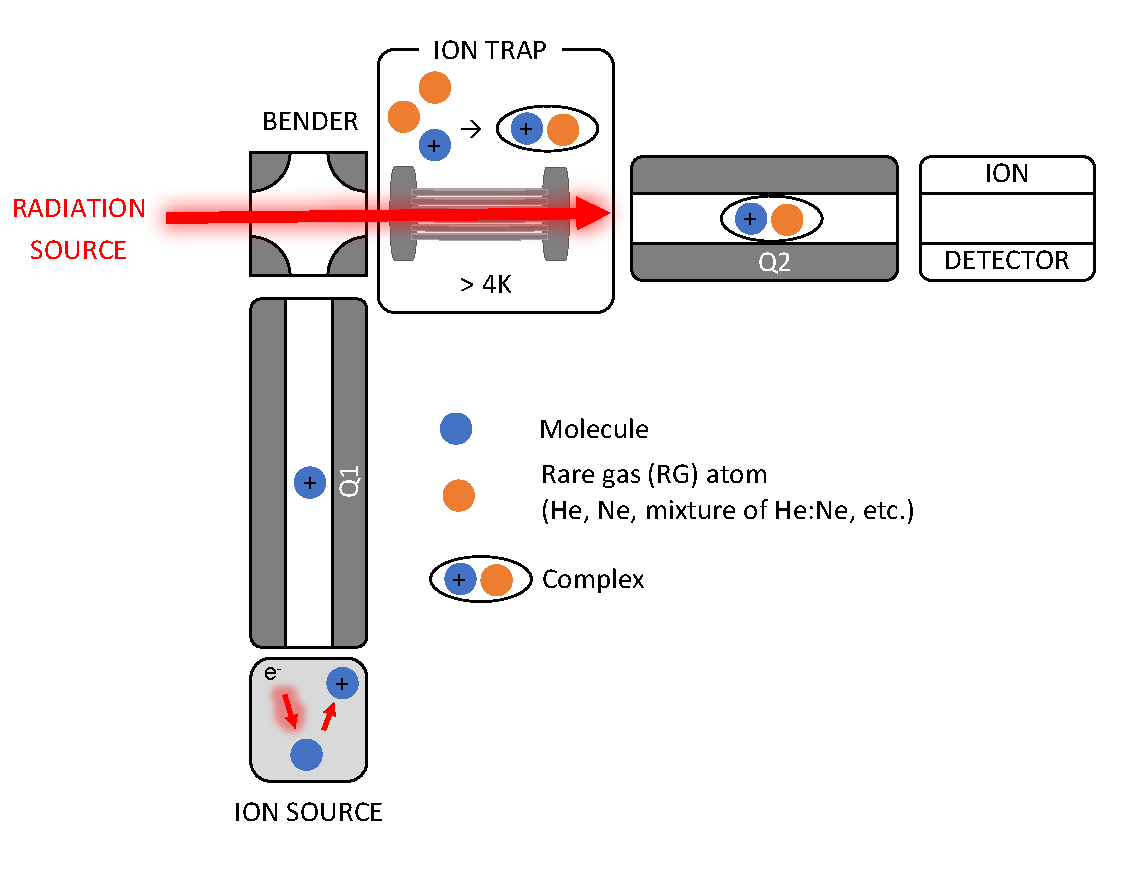
\includegraphics[width=1\textwidth]{figures/Instruments/FELion_schematics.pdf}
    
    \caption{Schematic drawing of the FELion ion trap setup. The 22-pole ion trap is coupled in-between two quadrupole mass filters (Q1 and Q2). The ions are guided into the trap from Q1 via quadruple bender (labelled BENDER). The trap contents are extracted after irradiation from the radiation source into Q2 to filter desired product molecular ions and then guided into a Daly type detector to be counted.}
    \label{fig:felion}
\end{figure}

The various spectroscopic and kinetics experimental studies reported in this thesis have been performed using the 22-pole cryogenic ion trap instrument (referred to as FELion), which has been built in the Cologne Laboratory Astrophysics group and installed permanently at the widely tunable \qt{Free Electron Lasers for Infrared eXperiments} (FELIX) \cite{oepts_free-electron-laser_1995} in Nijmegen, The Netherlands. As shown in the schematic diagram (Figure \ref{fig:felion}), the FELion instrument consists of an ion source, quadruple mass filters, an ion trap and a detector. A detailed description of the FELion instrument has been given by \citet{asvany_coltrap_2014}, \citet{kluge_state-selective_2016} and \citet{jusko_felion_2019}. This section will provide a brief discussion focusing on the FELion instrumental apparatus used in this study.

\subsection{Ion source}
\label{subsec:setup:ion-source}

One of the main challenges when studying highly reactive molecular ions is their production. The primary molecular ions are produced in the ion source using electron ionisation (EI), where an energetic electron (typical $20-70$ eV) interacts with molecules. \citet{dempster_new_1918} first demonstrated this process for the solid phase and later \citet{bleakney_new_1929} for the gas phase molecules. The ionisation process produces dissociative and non-dissociative products, i.e., ionised fragments and ionised parent molecules, respectively. A short pulse of produced ions is then extracted into the first quadrupole (Q1) by applying an adjustable pulse on the exit electrode (referred to as B0, see Figure \ref{fig:setup:ion-source}). This section will discuss the types of ion sources coupled to the FELion instrument.\\

\begin{figure}[!htb]
    \centering
    \begin{subfigure}[b]{0.49\textwidth}
        \centering
        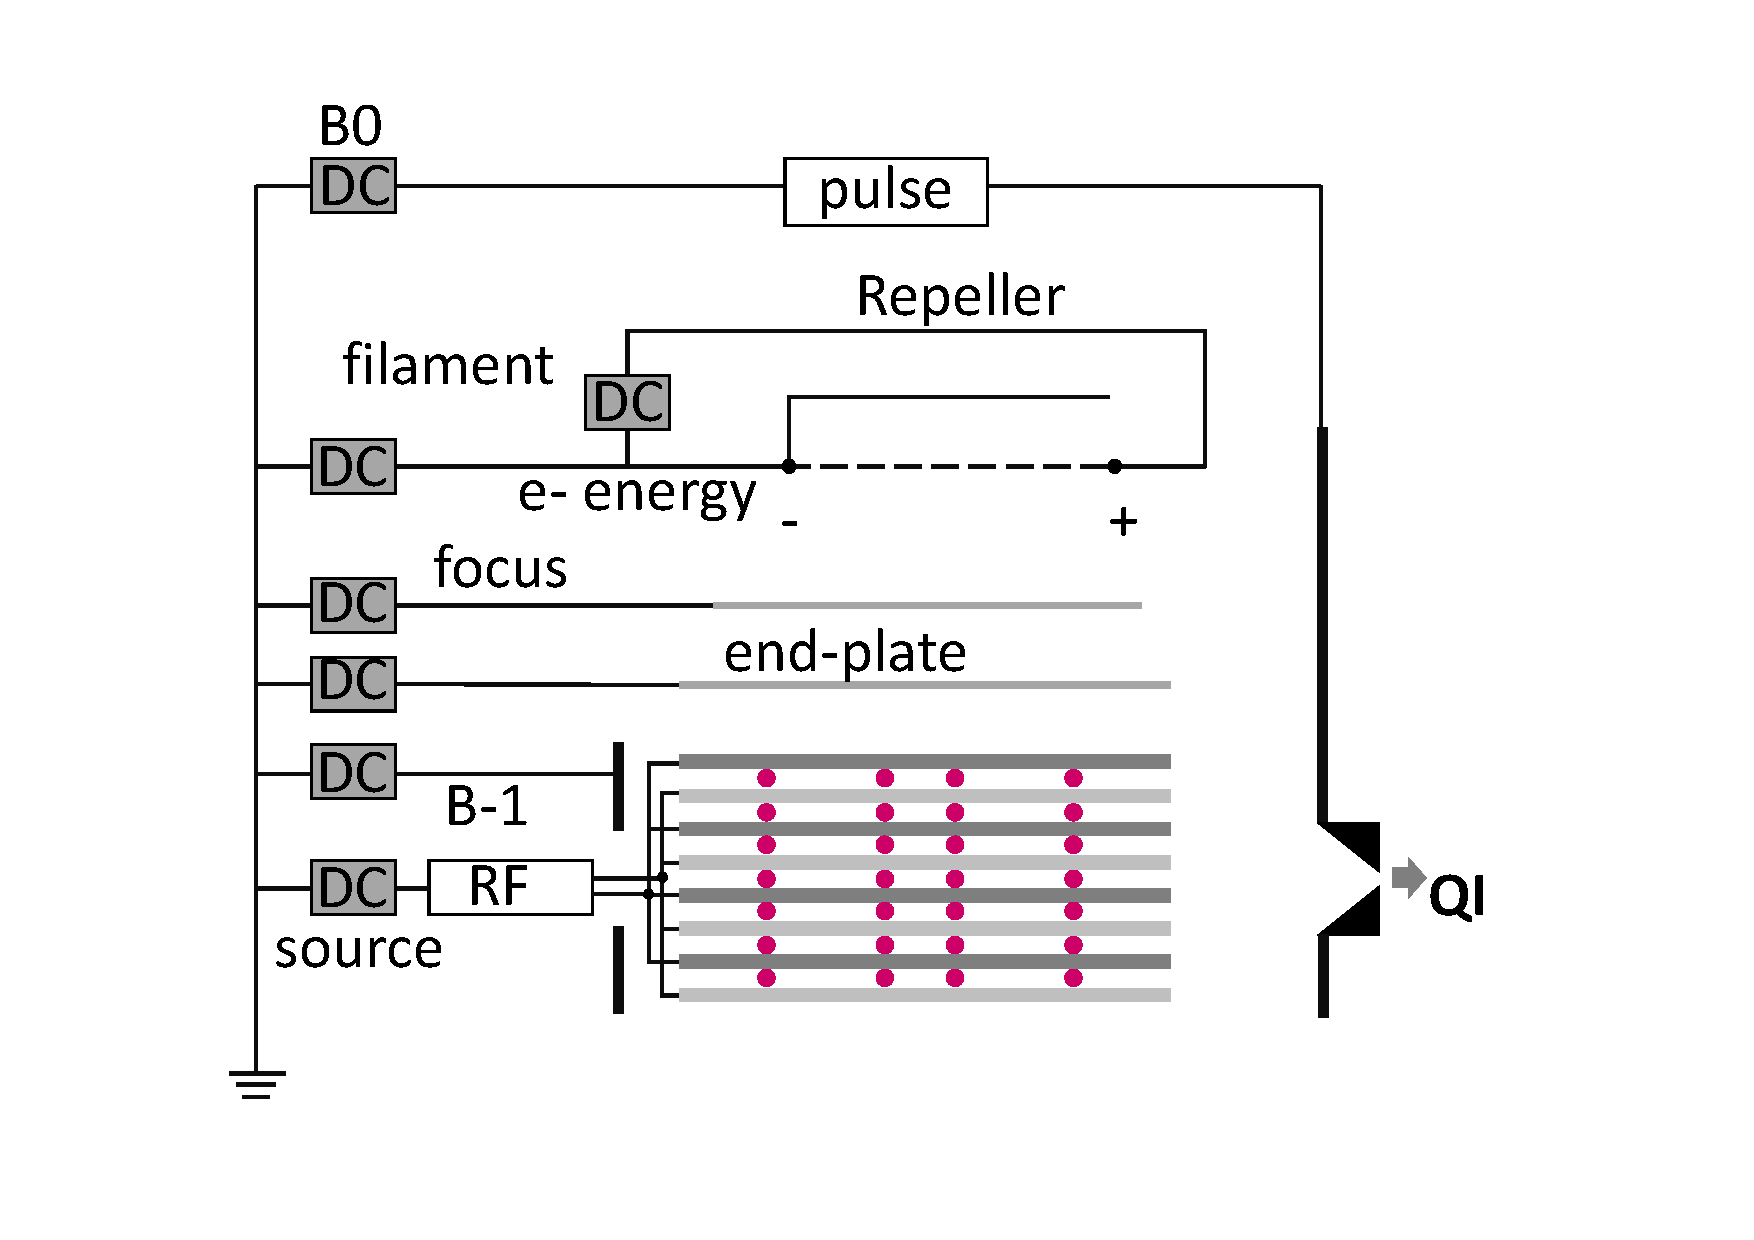
\includegraphics[width=1\textwidth]{figures/Instruments/ion-source/storage.pdf}
        \caption{}
        \label{fig:setup:storage-ion-source}
    \end{subfigure}
    \hfill
    \begin{subfigure}[b]{0.49\textwidth}
        \centering
        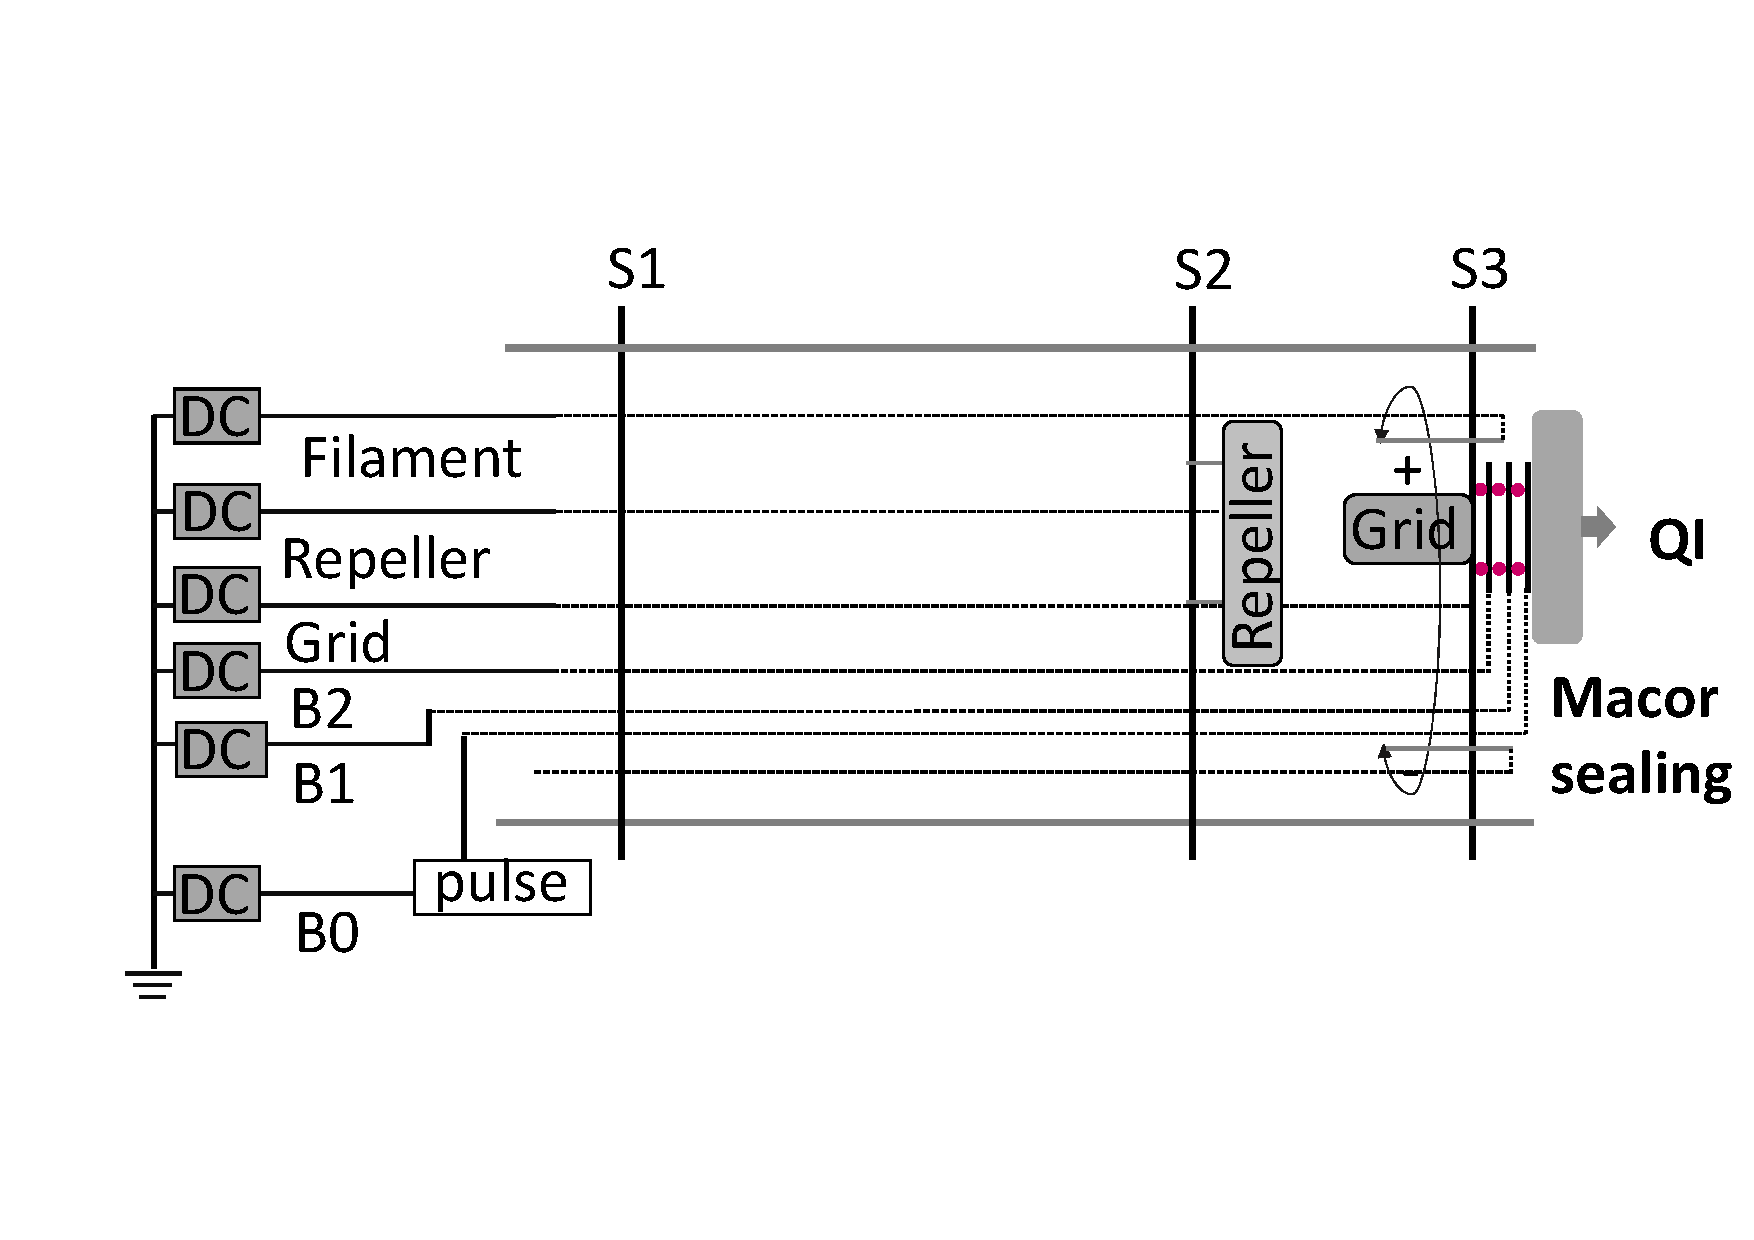
\includegraphics[width=1\textwidth]{figures/Instruments/ion-source/non-storage.pdf}
        \caption{}
        \label{fig:setup:non-storage-ion-source}
    \end{subfigure}
    \hfill
    \caption{Schematic drawing of the ion sources. The various components are labelled, and the corresponding connections are indicated by solid lines for (a) storage source and (b) non-storage (S1, S2 and S3 are grounded base plates for support). The pink circles represent ruby balls for insulation between connected electrodes. The labelled Macor sealing ring on top of the B0 electrode is placed to seal the ion source chamber and prevent any accidental contact between B0 and the Q1 rods.}
    \label{fig:setup:ion-source}
\end{figure}

\textbf{Storage source:} One type of ion source is a radiofrequency storage source, developed by \citet{gerlich_experimental_1992}. The primary ions are generated and stored ($\sim $s) in this source using an in-homogeneous RF field and DC potentials. The benefit of storing the ions in the source is that the produced molecular ions can undergo collisions with the background neutral gas or gas mixtures (typically at pressures of $10^{-6} - 10^{-5}$ mbar and a temperature of $\sim$ 400 K), leading to the production of secondary ions via chemical reactions and de-excitation and thermalization of the ions. 

As depicted in the schematic diagram (Figure \ref{fig:setup:storage-ion-source}), the storage ion source consists of a stack of eight \qt{double H-shaped} molybdenum plates (1 mm thickness), which are connected and electrically insulated by ruby balls (1 mm diameter). Four of the eight plates are connected alternately, and a typical $50-280$ V RF voltage is applied. The filament wire (rhenium $99.97 \%$, 0.2 mm diameter) is covered by the \qt{repeller} and the \qt{focus}, which are made up of 0.5 mm thick molybdenum plates. The filament typically operates around $\sim$ 5 V and 2.8 A and is held on a negative potential corresponding to the electron energy. The repeller is connected to the negative end of the corresponding filament. The DC voltages applied to the \qt{focus} and \qt{repeller} help to focus and accelerate electrons into the source. The B0 and B-1 are mounted at the front and back of the source apertures, respectively. This combination helps to confine the ions in the axial direction of the source by applying corresponding DC-potentials. The B0 can be pulsed to generate a short pulse (typically 10-100 ms) of ions for the experiments.

\textbf{Direct EI source:} The other type of ion source is called \qt{direct EI}, which produces primary ions by \qt{direct electron ionisation} but they are not stored. This source is a simple combination of repeller, grid, filament and lens, as shown in Figure \ref{fig:setup:non-storage-ion-source}. The filament wire is made up of a 0.25 mm Rhenium wire mounted in a circular arrangement around the grid covering 270 deg arc length. The filament's power supply ($\sim$ 5 V / 2.8 A) is floated to $10-70$ eV and, together with the grid voltage ($1-4$ V), acts as an electron gun which accelerates the electrons to provide the necessary energy to ionise molecules in the grid region. The repeller (typically operated around $-5 to -15$ V) is mounted on a grounded base plate with ceramic insulators and helps to focus and accelerate electrons into the grid region. The einzel lens (electrodes) set up towards the end consists of B0, B1 and B2 electrodes (insulated by ruby balls) to confine the ions in the axial direction of the source by applying corresponding DC-potentials.

Depending on the nature of the study, storage and direct EI sources can be used accordingly. The storage ion source provides the benefit of storing the formed ion for a few seconds, thereby often quenching ions to the most stable isomeric form  and the electronic ground state by undergoing (reactive) collision with the background gas. Additionally, the storage source can produce secondary ions via reactions with the background gas, e.g., protonation reactions. An efficient protonation process is, for example, discussed in more detail in chapter \ref{chapter:CH3CNH+}. On the other hand, the direct EI source allows us to produce also energetically higher-lying isomeric forms of ions and to characterize, for example, their formation routes via dissociative ionization. In Chapter \ref{chapter:C3H3+}, a detailed investigation of two different isomers (cyclic and linear form) are discussed using both direct EI and storage ion source.

Once the ions are formed in the source, a short pulse of ions is extracted into the first quadrupole mass filter (Q1). Adjusting the RF and DC potential voltages can further isolate and guide the molecular ion of interest into the trap, as will be discussed in the following section.

\subsection{Ion trap and detector}
\label{subsec:setup:ion-trap-and-detector}

The heart of the FELion instrument is a 4 K cryogenic 22-pole ion trap coupled in-between two quadrupole mass filters (Q1 and Q2). The Q1 and Q2 are perpendicularly angled. Therefore, the produced mass-filtered target ions from Q1 are guided into the trap by passing via a quadrupole bender, as shown in Figure \ref{fig:felion}. The 22-pole ions trap's design details are described by \citet{asvany_note_2010}. The trap RF is generated using amplified output (10 W amplifier) of a direct digital synthesizer (DDS) and operated at the trap resonance of around $\sim 18.3$ MHz. 

\begin{figure}[!b]
    \centering
    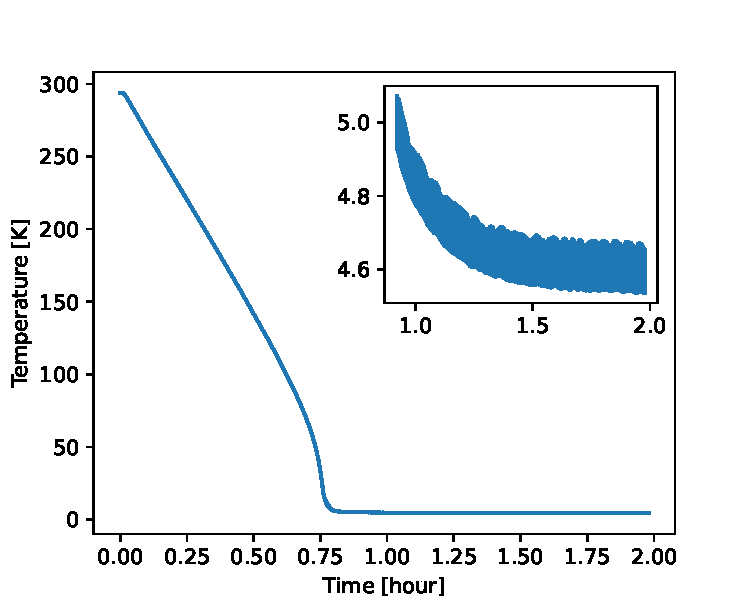
\includegraphics[width=0.9\textwidth]{figures/Instruments/cooldown-behaviour.pdf}
    \caption{Cool-down behaviour of the 22-pole cryogenic ion trap from room temperature using a He cryostat. The inset shows a detailed view of temperatures below 5 K.}
    \label{fig:cooldown_behaviour}
\end{figure}

The ion trap is mounted inside a copper housing and directly onto a cold head (Sumitomo RDK-408D2), allowing to cool it down to a minimum temperature of around 4 K using a He cryostat (see Figure \ref{fig:cooldown_behaviour}). The FELion instrument's 1 Hz machine cycle is synchronized with the cold head and FELIX laser (see Section \ref{subsec:ir:radiation-source}) for infrared experiments. The temperature can be varied between $5-40$ K using a thermo-strip (Kapton material, providing up to 40 W heating power) and monitored using an attached Si diode (Lakeshore DT-470-CU-13). The ions are kinetically and internally cooled by collisions with buffer gas atoms such as He or He:Ne mixture. However, it should be noted that the ion temperature is typically higher than the nominal trap temperature \cite{endres_incomplete_2017} (see Section \ref{subsec:collisional-ion-temperature}). The buffer gas is admitted directly into the trap region at high number densities ($10^{14}-10^{15}$ \percc, see Section \ref{subsec:numer-density} for number density measurements inside trap) either continuously or via a pulsed piezo valve depending on the experimental methods. 

The ions can be stored in the trap for up to 10 s (depending on the experiment) and then extracted from the trap. Subsequently, the parent or possible product ions are mass-selected with a second quadrupole mass filter (Q2) into a single-ion counting Daly type detector \cite{daly_scintillation_1960} for analysis. The pulses generated by the detector are amplified and discriminated (Phillips Scientific model 6906, 300 MHz) and counted with a gated 100 MHz counter (Ortec model 996).

In the next section, we shall discuss the spectroscopic methods employed in the 22-pole cryogenic ion trap (FELion instrument) for vibrational and rotational transition measurements of molecular ions.

\section{Vibrational spectroscopy}
\label{sec:methods:vibration}

\subsection{Experimental method}
\label{subsec:IRPD}

The action spectroscopic method employed to record the vibrational transitions of the molecular ions in this study is the well-known \qt{infrared predissociation (IRPD)} spectroscopy, as introduced in Section \ref{subsec:action:methods:vibrational:IRPD}.

In our IRPD experiment, the primary target ions are formed in the ion source and mass filtered into the 22-pole ion trap. A short He or He:Ne mixture pulse (50-100 ms) is introduced into the trap (typically at 4-9 K range). The molecular ion can form a weakly bound complex at low temperatures ($< 10$ K) and high number density ($10^{15}$ \percc ) via three-body collisions, as discussed in more detail in Section \ref{subsec:CD+-kinetics}. The tagging efficiency in forming the complex depends on the interaction strength between the molecular ion and the tag (He or Ne). This study typically obtains $> 10 \%$ tagging yield; more details on different molecular ions are described in their respective chapters. For tagging partners, the neon atom is often preferred, although the helium is better suited for IRPD studies due to its lower polarizability, lower binding energy, and thus  minimal perturbation on the ionic vibrational frequencies. However, for the same reason, since the He-complex is very weakly bound, it dissociates due to trap heating from a high-power radiation source, such as the free-electron laser employed in this study. The influence of the Ne tag on bare ion vibrational modes is discussed in corresponding chapters.

The trap contents are stored in the ion trap for about 1-2 s while being irradiated with pulsed IR radiation as a function of frequency, and the formed complexes are then mass filtered and counted. The dissociation of the complex at resonance transition yields the signal in the form of a depletion. The IR radiation source and data normalising procedures are described in the following sections.

\subsection{IR radiation source}
\label{subsec:ir:radiation-source}

The IRPD measurements for characterising the infrared signature of ionic complexes in this study are performed with two types of infrared (IR) radiation sources, the free-electron lasers FELIX and an optical parametric oscillator/amplifier (OPO/A) system. In this section, we shall briefly describe the interface of the FELion ion-trap instrument with these IR radiation sources.

\begin{figure}[!htb]
    \centering

    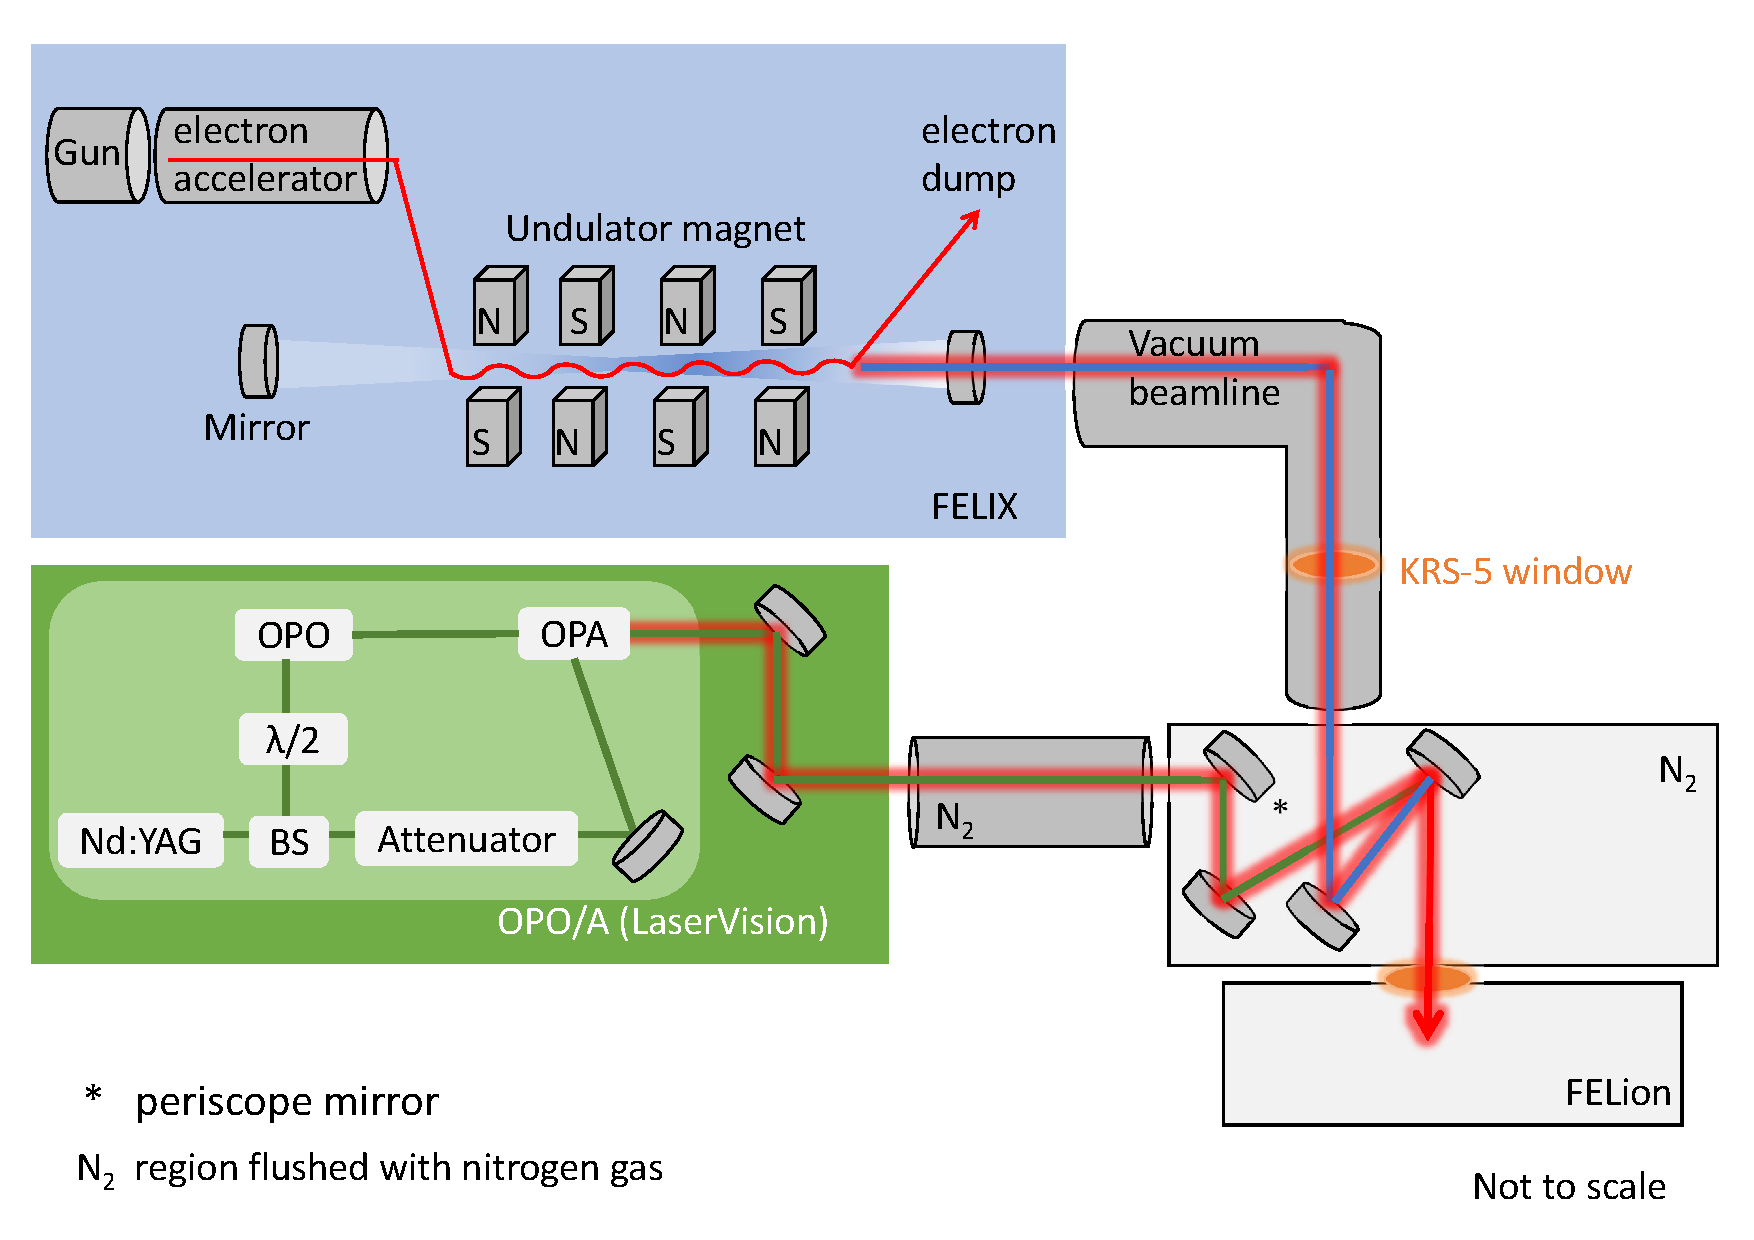
\includegraphics[width=1\textwidth]{figures/Instruments/FELIX-OPO-beamline.pdf}
    \caption{Schematic drawing of FELIX and OPO/A system interfaced with FELion user-station. The blue and green coloured lines represent the FELIX and OPO/A output laser beam paths, respectively. Only one system, FELIX or OPO/A, is operated at a given time.}
    \label{fig:FELIX}
\end{figure}

\subsubsection{FELIX} 
\label{subsec:ir:radiation-source:FELIX}

FELIX stands for \qt{Free Electron Lasers for Infrared eXperiment}; as the name suggests, it is a free-electron laser (FEL) facility, and the FELion instrument is located in its user-stations \cite{jusko_felion_2019}. This section briefly introduces the operating principles of an FEL, followed by a detailed description of the FELIX laser system coupled to the FELion instrument used in this study for infrared experiments.\\

\textbf{Operating principles:} In a conventional laser device, the laser light is generated through optical amplification based on the stimulated emission of electromagnetic radiation from e.g. an atomic or a molecular excitation. A free-electron laser system however employs relativistic electrons as a gain medium. As shown in Figure \ref{fig:FELIX}, an electron accelerator provides a beam of relativistic electrons followed by an undulator (periodic arrangement of magnets with alternating poles) in which the electrons perform a transverse oscillation and travel along the axis of the undulator. Two highly reflective mirrors form an optical laser resonator in which the radiation is amplified. By adjusting the electron beam's energy or the magnetic field strength of the undulator, the wavelength of the radiation emitted, $\lambda_r$ can be easily tuned and is given by \cite{oepts_free-electron-laser_1995}:

\[\lambda_r = \frac{\lambda_u}{2\gamma^2} \enclose{1 + \frac{K^2}{2}}\]

where $\lambda_u$ is the undulator wavelength (spatial period of the magnetic field), $\gamma$ is the relativistic Lorentz factor, and $K$ is the dimensionless parameter describing undulator magnetic strength.

The $\gamma$ and $K$ are defined as:
\begin{align*}
    \begin{split}
        \gamma &= \frac{1}{\sqrt{1-(v_z/c)^2}}\\
        K &= \frac{eB_u\lambda_u}{2\pi m_e c}
    \end{split}
\end{align*}
where $v_z$ is the velocity of the electron in the direction of the undulator, $c$ is the speed of light, $m_e$ is the mass of the electron, $e$ is the elementary charge, and $B_u$ is the applied magnetic field strength.\\

\textbf{FELIX laser system:} Currently, the FELIX laboratory consists of four laser systems, FEL-1, FEL-2, FELICE, and FLARE, each producing their range of wavelengths, and together, they provide a tuning range of 3-1500 $\mu$m. The FELion instrument is interfaced with the FEL-1 and FEL-2 pulsed IR laser system via an evacuated beamline with a wide tunable frequency range of 30-150 $\mu$m (330-66 \wn) and 3-45 $\mu$m (3330-220 \wn), respectively. FEL-2 delivers $> 2000$ \wn\ in $3^{rd}$ harmonic operation mode (FEL-2 was updated in 2022 after the experiments reported in this thesis have been concluded). The IR pulsed FELIX laser has a repetition rate of 10 Hz with a typical macropulse length of $\sim  10\ \mu$s and for the experiments reported here a 1 GHz micro-pulse structure (see Figure \ref{fig:FELIX-pulse}) has been used. 

\begin{figure}[!htb]
    \centering
    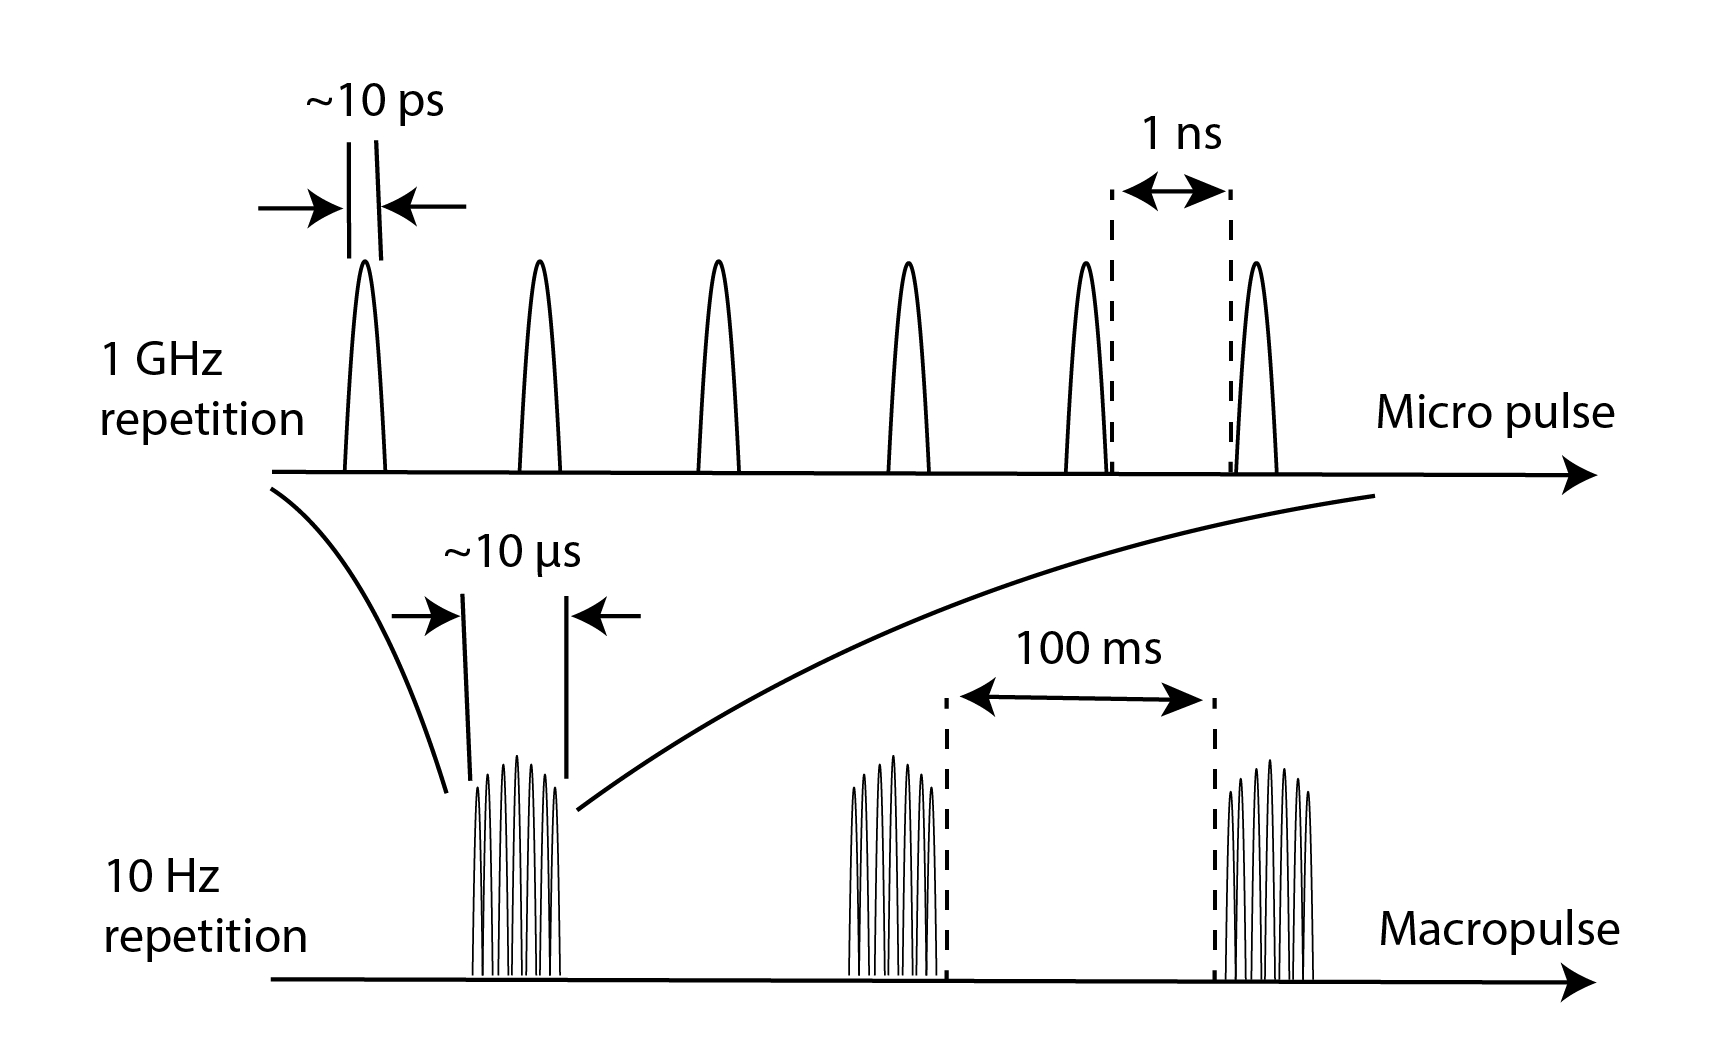
\includegraphics[scale=0.7]{figures/Instruments/FELIX-pulse-02.png}
    \caption{Schematic diagram of the FELIX laser micro and macro pulse structure.}
    \label{fig:FELIX-pulse}
\end{figure}

The maximum macro pulse output power reaching the user station is $> 50$ mJ. The full-width half maxima (FWHM) of radiation is Fourier-transform limited and can be on the order of $\Delta \nu = 5$ \wn\ at 1000 \wn. The schematic drawing of the free-electron laser (FELIX) interfaced with the FELion user station is shown in Figure \ref{fig:FELIX}. At the FELion user station, the IR radiation from FEL-2 is coupled into the FELion via two mirrors (one of them focuses the laser beam into the trap region) and two vacuum windows KRS-5 which permit photons down to 250 \wn\ with 75\% transmission. The KRS-5 windows are replaced with a PPE (beamline exit) and a CVD diamond window (FELion entrance) when FEL-1 is used. The region between the FELIX beamline and FELion is flushed with N$_2$ gas to avoid absorption in air.

\subsubsection{OPO/A}
\label{subsec:ir:radiation-source:OPO}

In addition to the FELIX laser system, the FELion instrument is coupled to a tunable OPO/A system (LaserVision, Narrowband OPO/A model).\\
\\
\textbf{Operating principles:}\\

The OPO/A system uses an optical parametric oscillator (OPO) and amplifier (OPA) 
instead of stimulated emission for optical gain. Hence, it consists of an optical resonator and non-linear crystals. 
It relies on two non-linear optical processes: second harmonic generation (SHG) and difference frequency generation (DFG).

The 1064 nm laser source (pump) input is split using a beam splitter, and one part ($1/3^{rd}$) is directed to the OPO 
stage and the other part ($2/3^{rd}$) to the OPA stage. Before entering the OPO stage, the 1064 nm input is frequency 
doubled via SHG to provide 532 nm input for OPO. In OPO, the input laser beam of frequency $w_p$ is split into two new 
lower energy photons via DFG using KTP crystals, called signal and idler, with frequency $w_s$ and $w_i$, respectively, 
such that $w_p = w_s + w_i$. The wavelengths of $w_s$ and $w_i$ can be tuned by phase-matching conditions (i.e., by 
changing the angle between the incident pump laser and optical axes of crystals). 

While in OPA, in addition to the initial $2/3^{rd}$ of 1064 nm pump beam input ($w_p$), 
the idler output ($w_i$) from OPO acts as a signal input beam for OPA. The signal and pump beam is then directed into
the non-linear KTA crystals of OPA. Subsequently, using DFG, generating high energy output beam 
with a tunable wavelength in the intermediate/mid-infrared region.\\

\noindent \textbf{Setup:}\\

The OPO/A system coupled to the FELion instrument is shown as a schematic diagram in Figure \ref{fig:FELIX}. This is a multi-stage nonlinear device designed to convert the fixed-frequency output of a seeded 1064 nm Nd:YAG pump laser (operated at 10Hz) into tunable radiation in the intermediate and mid-infrared, using the combination of a 532 nm pumped OPO followed by a 1064 nm pumped OPA. The system produces a tunable output (MIR Idler) from 2.218-5 $\mu$m, i.e., 2000-4500 \wn\ frequency range with a maximum pulse energy of up to 25 mJ and line bandwidth of $\sim 0.1$ \wn\ (seeded).

\subsection{Data analysis}
\label{subsec:ir:data-analysis}

This section will discuss the data processing, including calibration, normalization, and averaging process of the obtained spectra from the FELion instrument combined with FELIX. During the PhD work, an analysis software package called FELionGUI, based on Python 3 was developed \footnote{Vist \url{https://felion-docs.vercel.app/} for FELionGUI documentation}.\\

\begin{figure}[!htb]
    \centering
    
    \begin{subfigure}[b]{0.45\textwidth}
        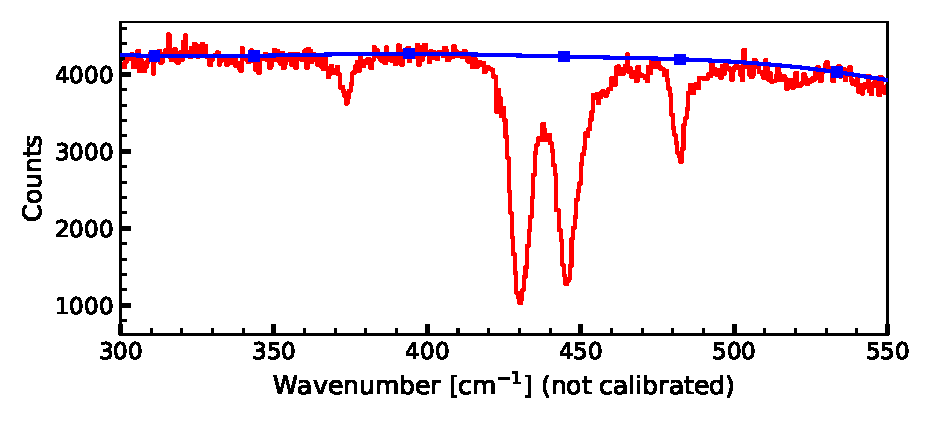
\includegraphics[width=1\textwidth]{figures/IR-data-norm/baseline_correction.pdf}
        \caption{}
        \label{fig:data-process:raw}
    \end{subfigure}
    \hfill
    \begin{subfigure}[b]{0.45\textwidth}
        \centering
        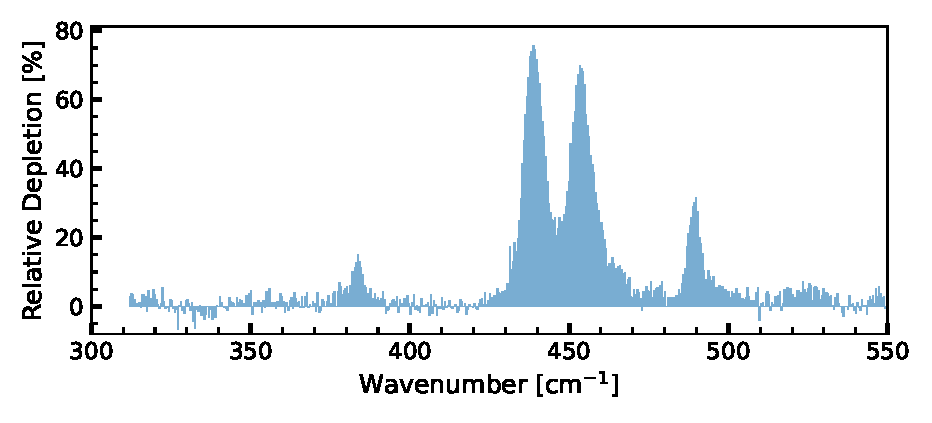
\includegraphics[width=1\textwidth]{figures/IR-data-norm/processed.pdf}
        \caption{}
        \label{fig:data-process:processed}
        \end{subfigure}
    \hfill
    % \begin{subfigure}[b]{0.45\textwidth}
    %     \centering
    %     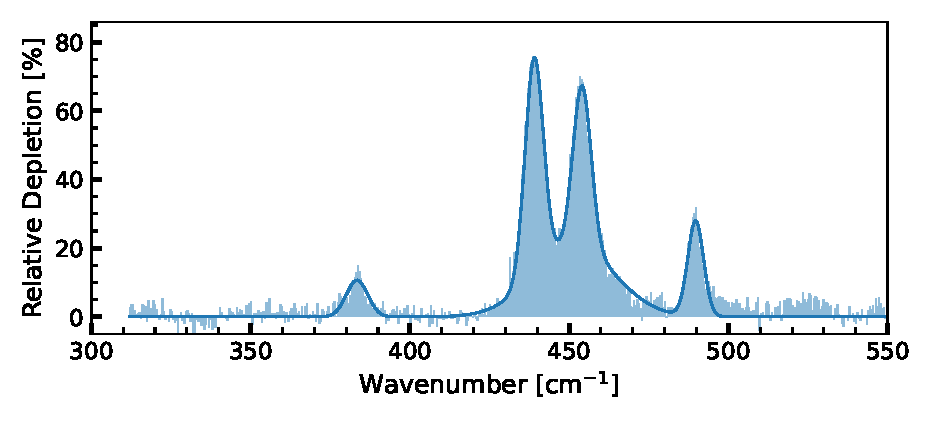
\includegraphics[width=1\textwidth]{figures/IR-data-norm/fitted.pdf}
    %     \caption{}
    %     \label{fig:data-process:fitted}
    %     \end{subfigure}
    % \hfill
    \begin{subfigure}[b]{0.45\textwidth}
        \centering
        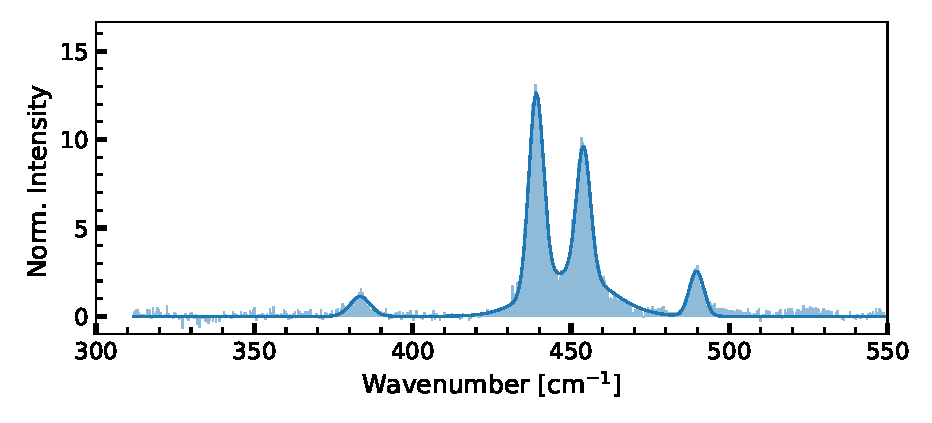
\includegraphics[width=1\textwidth]{figures/IR-data-norm/normalised.pdf}
        \caption{}
        \label{fig:data-process:normalised}
    \end{subfigure}
    
    \caption{Data processing (for Ne-HC$_3$N$^+$ IRPD spectrum using FELIX): (a) is the raw data obtained by directly measuring the depletion counts of formed complex ions in IRPD schemes at varying frequencies. The blue line corresponds to a possible baseline to account for ion count fluctuation. (b) is the first processed spectrum with baseline correction from (a). (c) is the final normalised spectrum (see text) and the solid line corresponds to fitting the spectrum with a multi-component Gaussian function.}
    \label{fig:data-process}
\end{figure}

\textbf{Baseline correction:} The formed ion complex is monitored and counted in the IRPD experiments reported in this thesis. Figure \ref{fig:data-process:raw} shows the measured raw data. Each data point is typically an average of 4 iterations. This spectrum should be baseline corrected for ion count fluctuation. Since even slight changes in the experimental condition, such as temperature, number density, and change in tagging efficiency due to laser heating, etc., can induce a non-linear shift in an otherwise constant background signal. As shown in Figure \ref{fig:data-process:raw}, the solid blue line is the constructed baseline via a cubic spline interpolation and can be manually adjusted. In addition to baseline correction, the raw spectrum needs to be frequency calibrated against the actual frequency output from the radiation source, i.e., using a grating spectrum analyser (FELIX) and manual wavenumber corrections based on a wavemeter (HighFinesse WS - Series) reading (OPO/A system).\\

\textbf{Normalisation and fitting:} Initially, baseline corrected data is a relative depletion ($D$) of complex ions and is given by:

\[ D= 1 - \frac{N_{ON}(\nu)}{N_{OFF}} \] 

where $N_{OFF}$ is the baseline value and $N_{ON}(\nu)$ is the depleted value of the number of complex ions that are observed upon resonant vibrational excitation as shown in Figure \ref{fig:data-process:processed}.

To account for variations of the laser pulse energy $E$, pulse number $n$, and for saturation effects, the signal is normalised ($I$) as given below: 

\[ I [\text{per J}]=\frac{- ln(N_{ON}(\nu)/N_{OFF})}{n \cdot E[\text{in J}]} \]

where $I$ is the intensity in units of relative cross-section per Joule. 

One can obtain a relative cross-section per photon by multiplying $I$ with the wavenumber. Figure \ref{fig:data-process:normalised} shows the final normalised spectrum. The measurements are repeated in the same frequency range for averaging, i.e., the final spectrum is obtained by averaging using statistical binning with a typical bin size of 1.5-2 \wn\ of all normalised data. Line parameters such as band positions, intensities, and line widths (fwhm) are then obtained with statistical errors by fitting a multi-component Gaussian function to the experimental data. 

\section{Rotational spectroscopy}
\label{sec:methods:rotation}

\subsection{Experimental method}
\label{subsec:ROSAA}

The ROSAA action spectroscopic technique is employed in this work to record pure rotational transitions. In this section, we shall discuss this technique in detail.

Initially, the primary target molecular ions are produced from an ion source (see Section \ref{subsec:setup:ion-source}) by electron ionization from a neutral precursor using either storage or non-storage ion sources. A short pulse of the isolated molecular ion of interest is injected into the trap and stored for a specified time, typically $\sim 600$ ms for rotational action spectroscopic experiments, with continuous inflow of either pure He or He:Ne mixture buffer gas for collisional cooling and complex formation. At low temperatures (around 5-6 K and 6-15 K trap ambient temperature for helium and neon tag, respectively) and high number density $\sim10^{14}$ \percc\ of gas inflow, the buffer gas atoms will readily attach to the target ion by ternary association and can dissociate by collision-induced dissociation.

The ROSAA technique utilises the change in the rare gas atoms' attachment rate to a molecular ion (M$^+$) depending on its internal excitation, i.e., ions with a rotational quantum number $J$ have different attachment rate coefficients for forming HeM$^+$ clusters (see Section \ref{subsec:ROSAA-simulation}). The ternary association and collision-induced dissociation rate coefficients can be experimentally measured by following corresponding reactant and product ion counts as a function of trap time. These rate coefficients are a weighted averaged rate coefficient over the thermal population of rotational levels, i.e., the Boltzmann distribution close to the nominal trap temperature, reached by He collisional excitation rates of the order of $\sim 10^4$~s$^{-1}$ at the typical number densities ($\sim 10^{14}$ \percc) used in these experiments. Upon resonant excitation, the thermal equilibrium distribution is disturbed by competing radiative processes (typically with comparable rates of $\sim 10^5$~s$^{-1}$ for the M$^+$ rotational transitions), leading to a change in the attachment rate and thus the number of formed complexes. Hence, the measured signal intensity ($S$) is given as the observed change (in \%) of the number of He-M$^+$ complexes formed between the set frequency ($I_{ON}$) and a fixed reference frequency ($I_{OFF}$, offset about 3 $\sim$ GHz from scanning range), and scaled by $I_{OFF}$, i.e., $ S=(I_{OFF} - I_{ON})/I_{OFF} $, after storing for a fixed time of typically $\sim$ 600 ms in the trap at each data point (see Sections \ref{subsec:rot:radiation-source} and \ref{subsec:rot:power} for radiation source details). The spectra are measured in typically $10\sim$ kHz steps.

\subsection{THz radiation source}
\label{subsec:rot:radiation-source}

A continuous wave Signal Generator Extension (SGX) Module (VDI - Virginia Diode, Inc. WR9.0-SGX) has been used to measure pure rotational transitions of molecular ions. The SGX covers the frequency range from 82.5 - 1100 GHz using different frequency doubler or tripler combinations. Table \ref{tab:vdi-multiplier} provides the configurations used in this thesis. The microwave signal generator (R\&S \textsuperscript{\textregistered} SMB100A up to 40 GHz) drives the SGX and is disciplined by an atomic clock (Stanford Research Systems - FS740), such that the intrinsic radiation linewidths are better than 1~kHz, and the relative frequency accuracy is specified to be better than $1\cdot 10^{-13}$. The WR9.0 SGX was placed directly in front of a $\sim$ 0.6 mm thick CVD diamond window (Diamond Materials GmbH) with a conical/diagonal horn antenna and directed into the trap region. Figure \ref{fig:power-curves} shows the power output measured using a high sensitivity thermal sensor (3A-P-THz Ophir photonics) for configuration WR9.0 and WR2.2 SGX.

\begin{threeparttable}[!htb]
    \centering
    \caption{WR9.0M-SGX configuration details at standard RF input mode. }
    \begin{tabular}{cccc}
        \hline\\
        Designation & Frequency [GHz] & Configuration & N\tnote{*} \\
        \\\hline\hline\\
        WR9.0 & 82.5-125 & WR9.0SGX & 9 \\
        WR4.3 & 170-250 & WR9.0SGX + WR4.3X2 & 18 \\
        WR2.2 & 340-500 & WR9.0SGX + WR4.3X2 + WR2.2X2 & 36 \\
        \\\hline\hline
    \end{tabular}
    \begin{tablenotes}
        \item[*] N indicates the multiplier for signal generator (R\&S \textsuperscript{\textregistered} SMB100A) frequencies.\\
    \end{tablenotes}
    \label{tab:vdi-multiplier}
\end{threeparttable}

\begin{figure}[!htb]
    \Subfigure[0.48]{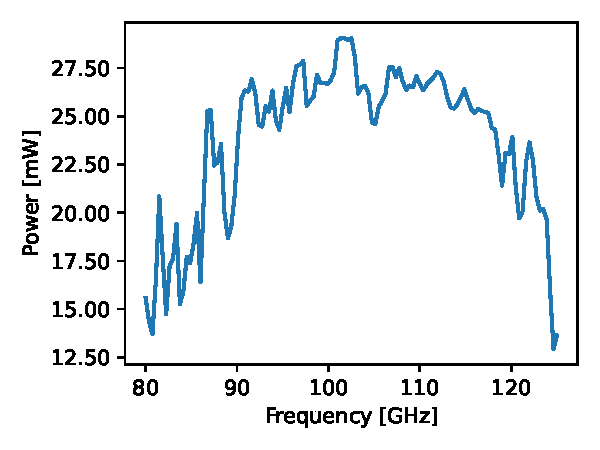
\includegraphics[width=1\textwidth]{figures/measurements/power-curves/WR9.0M.pdf}}{WR9.0}{\label{fig:power-curve:WR9.0}}
    \hfill
    \Subfigure[0.48]{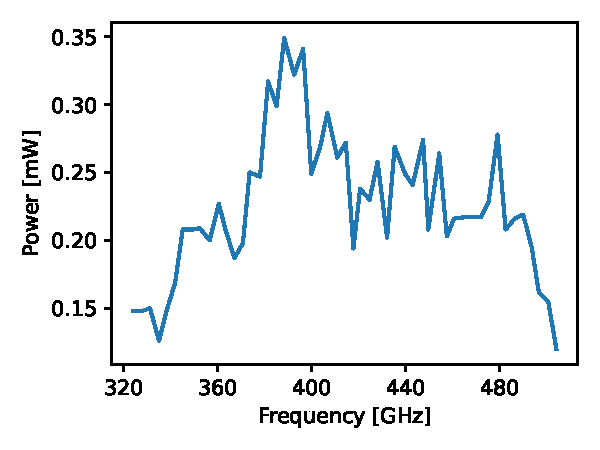
\includegraphics[width=1\textwidth]{figures/measurements/power-curves/WR2.2.pdf}}{WR2.2}{\label{fig:power-curve:WR2.2}}
    \hfill

    \caption{Power curves measured with Virginia Diodes, Inc. (VDI) WR9.0 Modular SGX Modules in (a) WR9.0 and (b) WR2.2 configuration as described in Table \ref{tab:vdi-multiplier}.}
    \label{fig:power-curves}
\end{figure}

\begin{figure}[!htb]
    \Subfigure[0.3]{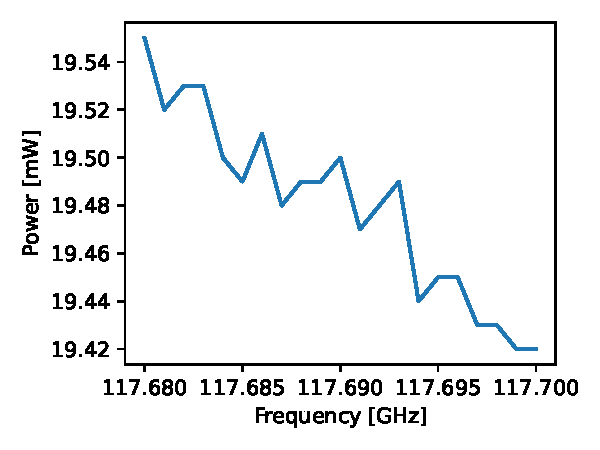
\includegraphics[width=1\textwidth]{figures/measurements/power-curves/WR9.0M_117GHz.pdf}}{}{}
    \hfill
    \Subfigure[0.3]{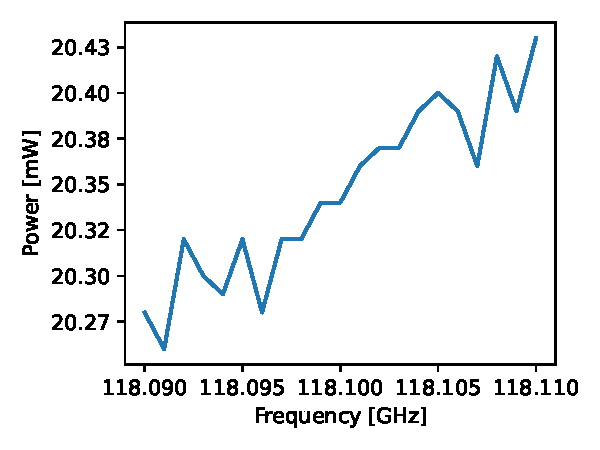
\includegraphics[width=1\textwidth]{figures/measurements/power-curves/WR9.0M_118GHz.pdf}}{}{}
    \hfill
    % \centering
    \Subfigure[0.3]{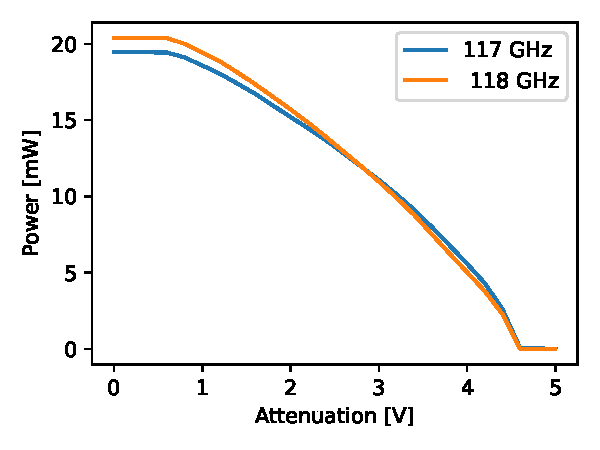
\includegraphics[width=1\textwidth]{figures/measurements/power-curves/WR9.0M_117GHz _att_WR9.0M_118GHz _att.pdf}}{}{\label{fig:power-attenuation-117-118}}
    \hfill
    \caption{Power curves measured with Virginia Diodes, Inc. (VDI) WR9.0 Modular SGX Modules in WR9.0 configuration, for the frequency ranges (a) $117.68-117.70$ GHz and (b) $118.09-118.11$ GHz. (c) shows the user-controlled attenuation power output for (a) and (b) as labelled 117 and 118 GHz, respectively. }
    \label{fig:power-attenuation}
\end{figure}

The maximum radiation output power can be regulated using \qt{User Controlled Attenuation (UAC)}. The UCA voltage reduces the SGX module's output power. Figure \ref{fig:power-attenuation} shows the WR9.0 SGX module output power as a function of UAC voltage from  $0-5$ V using a DC power supply (0 V = no attenuation, 5 V = full attenuation). The maximum output power reaching the trap centre region is discussed in the following section \ref{subsec:rot:power}.

\clearpage

\subsection{Determining the radiation power at the trap region}
\label{subsec:rot:power}

\input{chapters/technical-details/figs/power-curve-453GHz/feed-horn}

The feed horn antenna's electric field radiation emitted/propagated is shown in
Figure \ref{fig:feed-horn}. The propagation of the emitted Gaussian beam radius
($w(z)$) from a horn antenna is given by:

\input{chapters/technical-details/figs/power-curve-453GHz/beam_propagation}

\begin{equation}
    w(z) = w_0 * \sqrt{1 + \left( \frac{z}{Z_R} \right) ^2}
    \label{eqn:beam-propagation}
\end{equation}
where $Z_R$ is the Rayleigh length (or Rayleigh range) for Gaussian beams.

$Z_R$  is determined by the waist radius $w_0$ and the wavelength ($\lambda$) as shown below:

\[Z_R = \frac{\pi \cdot w_0^2}{\lambda}\]

Using a diagonal horn antenna (VDI waveguide band WM-570) of length, aperture
diameter and beam waist radius of 36, 3.6 and 1.5 mm, respectively. The
Gaussian beam propagation simulation for a frequency $\Delta \nu = 453$ GHz is
shown in Figure \ref{fig:power-curve:beam-propagation}.

\input{chapters/technical-details/figs/power-curve-453GHz/beam_propagation_power_curve}

As the Gaussian laser beam propagates, the waist radius increases in size and
the corresponding intensity profile of the electric field is given by:

\begin{equation}
    \begin{split}
        I(r) & = I_0 \cdot exp \left[ -2 \left (\frac{r}{w(z)}\right ) ^2\right] \\
        & = \frac{2P}{\pi w(z)^2}
        \cdot exp \left[ -2 \left (\frac{r}{w(z)}\right ) ^2\right]
    \end{split}
    \label{eqn:beam-propagation:intensity}
\end{equation}

where $I_0$ is the peak irradiance at the centre of the beam, r is the radial
distance away from the propagation axis, w(z) is the radius of the laser beam
where the irradiance is 1/e$^2$ (13.5\%) of $I_0$, z is the distance propagated
from the plane where the wavefront is flat, and P is the total power of the
beam.\\

Figure \ref{fig:power-curve:beam-propagation-power} shows the intensity profile
using Eq. \ref{eqn:beam-propagation:intensity}, when the beam waist radius,
$w(z)=2.5$ cm, is at the trap entrance (see Figure
\ref{fig:power-curve:beam-propagation}). Since the ion-trap aperture diameter
is 0.3 cm which is much narrower compared to the incoming beam radius (2.5 cm),
one needs to consider an offset for the Gaussian beam centre reaching the trap
centre. Therefore, the figure \ref{eqn:beam-propagation:intensity} also
features the orange marked region, which indicates the actual power estimated
to reach the trap depending on its alignment, $r(z)$, \emph{w.r.t} the
propagating Gaussian beam centre, $r_0(z)$. If we assume that in our
experiment, $r(z)=0-1.5$ cm, then the final radiation power reaching the trap,
for $\Delta \nu=453$ GHz frequency is 9-19 \% of the peak power (250 $\mu$W),
i.e., $35(12)\ \mu$W.

% However, one can 100 \% focus the beam into the trap using a combination of radiation source and optics. The optics design and details are discussed in Section \ref{subsec:THz-optics}.
\subsection{Determining the collisional ion temperature}
\label{subsec:collisional-ion-temperature}

In the spectroscopic experiment to investigate pure rotational transitions, the ions are cooled down in the trap by collisions with a buffer gas atom such as He, Ne or He:Ne mixture. The collisional ion temperature (T$_{\text{coll}}$), i.e., translational or kinetic temperature of the ions in the trap, which corresponds to mean collisional energy between the partners, thus the neutral buffer gas and the molecular ion, is an important factor to be determined especially for the models described in Section \ref{subsec:ROSAA-simulation} . This temperature cannot be measured directly but can be estimated by:

\begin{equation}
    \text{T}_{\text{coll}} = \frac{\text{m}_\text{He} \cdot \text{T}_{\text{ion}}  + \text{m}_\text{ion} \cdot \text{T}_{\text{He}} }{\text{m}_\text{He} + \text{m}_\text{ion}}
    \label{eqn:Tcoll}
\end{equation}

where \qt{m} is mass and \qt{T} is temperature, and the subscript \qt{He} and \qt{ion} indicates the corresponding buffer gas atom used (helium in this case) and the molecular ion of interest, respectively. The nominal trap temperature measured is assumed to be T$_{\text{He}}$. However, it has to be noted that the ion temperature (T$_{\text{ion}}$) is often higher than the nominal trap temperature \cite{endres_incomplete_2017}. Furthermore, T$_{\text{ion}}$ can be measured via the Doppler width estimated from the recorded full-width half maxima (FWHM) of a rotational transition at a given power. The measured rotational line profile corresponds to the Voigt profile, which is a convolution of a Gaussian profile (due to the kinetic energy distribution of the ions) and a Lorentzian profile (caused by power broadening). The FWHM of the Gaussian ($f_G$) and Lorentzian ($f_L$) profile can be derived as follows:


\begin{equation}
    f_G = \nu \cdot \sqrt{\frac{8 \cdot \text{k}_b \cdot \text{T}_{ion} \cdot \text{ln}(2)}{\text{m}_{ion} \cdot c^2}} = \text{C}_G \cdot \sqrt{\text{T}_{ion}}
    \label{eqn:fG}
\end{equation}

where $\nu$ corresponds to the central line frequency of the profile and C$_G$ is the Doppler proportionality constant, and by:

\[ f_L = \frac{\sqrt{2}}{2 \cdot \pi} \cdot \Omega _R \]
substituting angular Rabi frequency of the transition, which is defined as, $\Omega _R$ = \( \frac{\mu \cdot \text{E}}{\hbar} \) \footnote{$\mu$ is transition dipole moment, and E is the electric field, hence dividing the energy term $(\mu \cdot \text{E})$ by $\hbar$ gives angular frequency}, we get

\[ f_L = \frac{\sqrt{2}}{2 \cdot \pi} \cdot \frac{\mu \cdot \text{E}}{\hbar} \]

Substituting electric field strength, 
\( \text{E} = \sqrt{\frac{2\cdot I}{c \cdot \epsilon _0}} \)
where \emph{I} is the intrinsic intensity 
\( I = \frac{1}{2} \cdot c \cdot \epsilon _0 \cdot \text{E}^2 = \frac{P}{A_{trap}} \), 
we get the final expression for Lorentian FWHM, f$_L$:

\begin{equation}
    f_L = \frac{2\cdot \mu}{h} \sqrt{\frac{P}{A_{trap} \cdot c \cdot \epsilon _0 }} = C_P \cdot \sqrt{P}
    \label{eqn:fL}
\end{equation}
where \emph{P} is the output radiation power in W, $A_{trap} = 5 \cdot 10^{-5} $cm$^2$ is the trap area and $C_P$ is a power-broadening proportionality constant.\\

The Voigt profile is given by: 
\begin{equation}
    V(x; \sigma, \gamma) = \frac{Re[W(z)]}{\sigma \sqrt{2\pi}}
    \label{eqn:VoigtProfile}
\end{equation}

where $\sigma$ is the standard deviation in Gaussian profile, $\gamma$ is the half-width half maxima of Lorentzian profile and $Re[W(z)]$ is the real part of the Faddeeva function.

\begin{equation}
    \sigma = \frac{f_G}{2\sqrt{2\cdot ln(2)}}
    \label{eqn:fG-sigma}
\end{equation}
\begin{equation}
    \gamma = \frac{f_L}{2}
    \label{eqn:fL-gamma}
\end{equation}
\[ z = \frac{x + i\gamma}{\sigma \sqrt{2}} \]

The FWHM of Voigt profile can be approximated  with an accuracy of 0.02\% by \cite{olivero_empirical_1977}:

\begin{equation}
    f_V = 0.5346 \cdot f_L + \sqrt{0.2166 \cdot f_L^2 + f_G^2}
    \label{eqn:fV}
\end{equation}

To determine T$_{\text{ion}}$, the experimentally measured rotational spectrum is fitted with the Voigt profile (Eq. \ref{eqn:VoigtProfile}); subsequently, line parameters $\sigma$ and $\gamma$ are obtained. Using $\sigma$, one can compute $f_G$ using Eq. \ref{eqn:fG-sigma} and finally, T$_{\text{ion}}$ from $f_G$ using Eq. \ref{eqn:fG}.

\subsection{Numerical simulation}
\label{subsec:ROSAA-simulation}

The ROSAA action spectroscopic technique, as described in Section \ref{subsec:ROSAA} utilises the change in attachment rate of rotation-specific energy levels to record the pure rotational spectrum. As depicted in Figure \ref{fig:setup:ROSAA} there are several competing processes involved in affecting the molecular ion population distribution on different rotational levels, and consequently affecting the obtained signal intensity. Therefore, in this section, the processes depicted in Figure \ref{fig:setup:ROSAA} will be described in detail. Consequently, we discuss a kinetic numerical model approach to understanding the ROSAA signal intensity.

\begin{figure}[!htb]
    \centering
    
    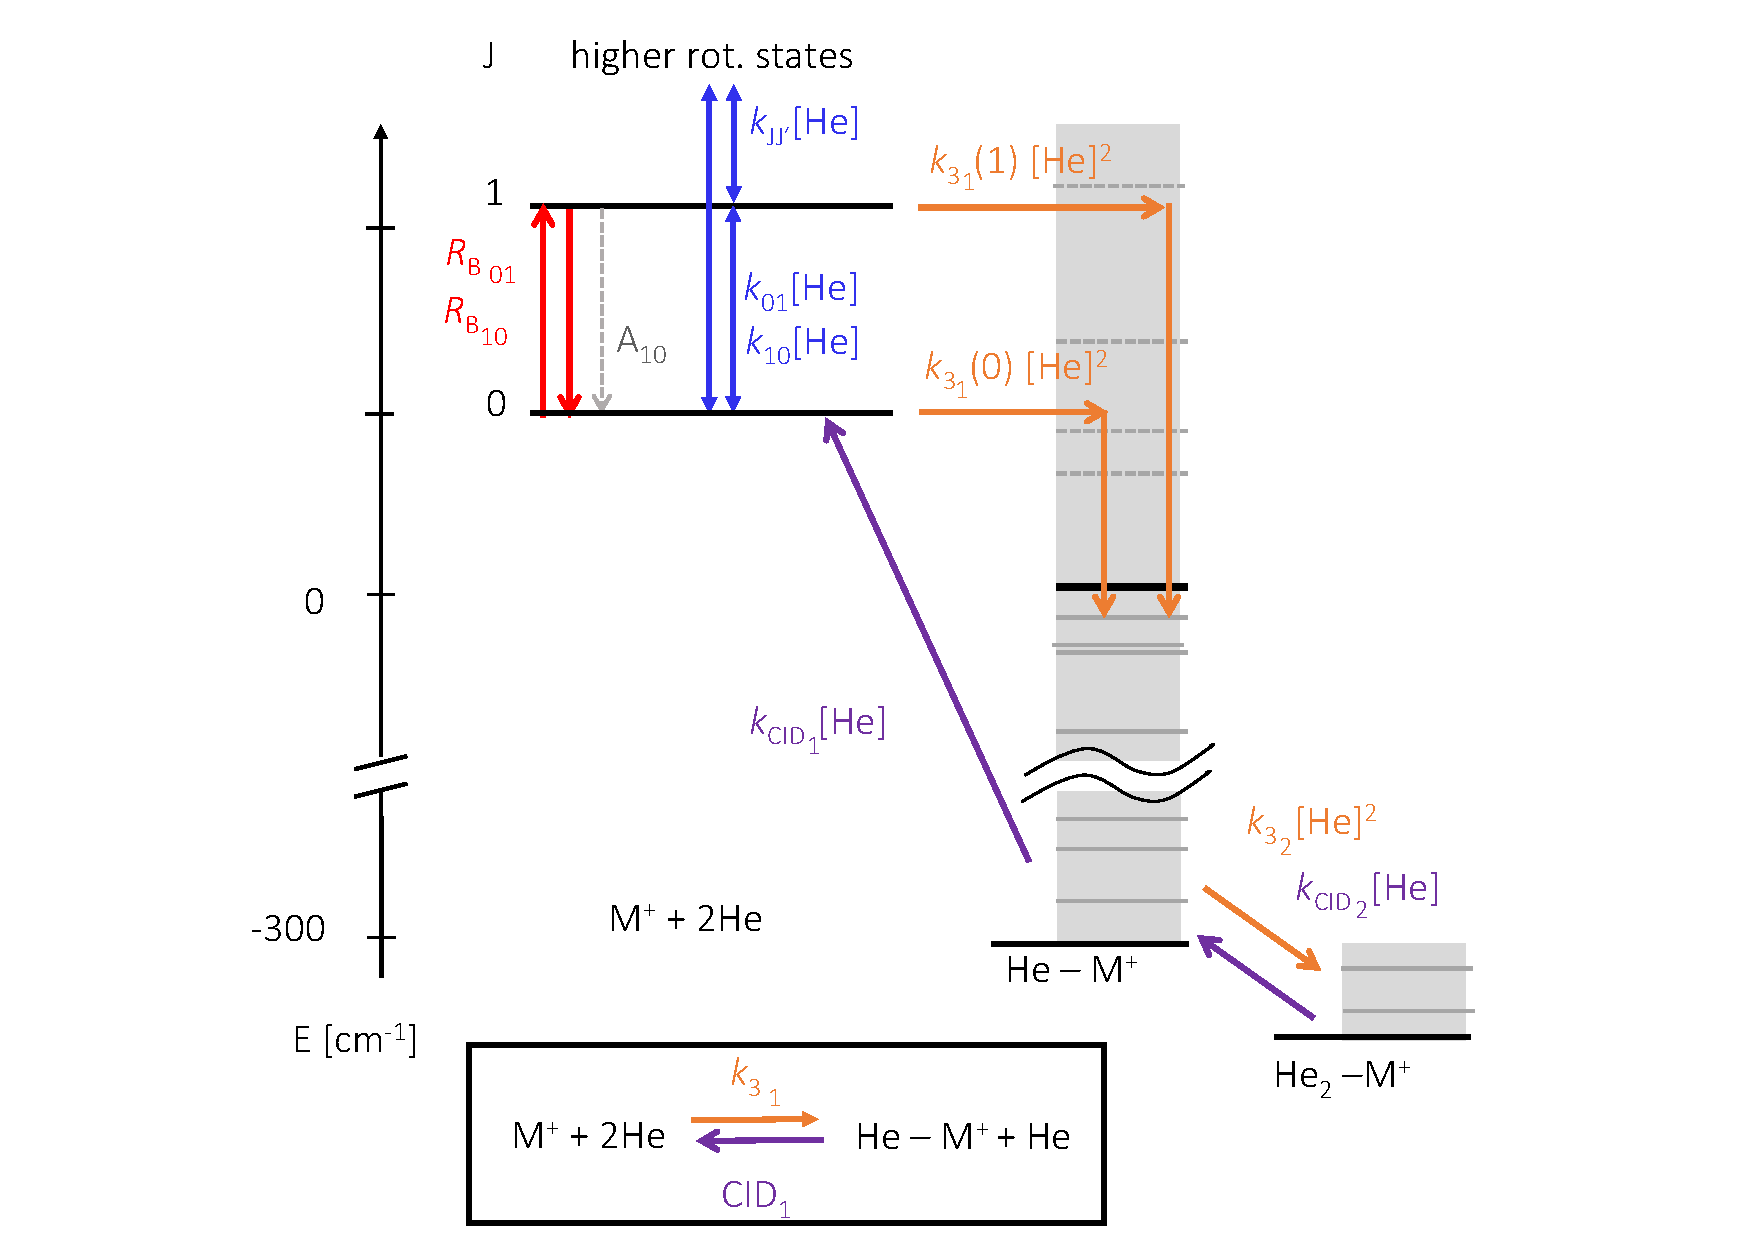
\includegraphics[width=1\textwidth]{figures/methods/ROSAA.pdf}
    \caption{Schematic kinetic model of the ROSAA action spectroscopic technique. The coloured labels and arrows indicate several competing processes for the reaction between the molecular ion M$^+$ and the neutral He atom. The typical rates for collisional (\textcolor{blue}{blue}) and radiative process (\textcolor{red}{red}) are in the range of $10^{4} - 10^{5}$ \pers, effective binary complex formation (\textcolor{orange}{orange}) is $> 0.01$ \pers\ and the collision-induced dissociation (\textcolor{violet}{violet}) is $> 0.1$ \pers\ at a given number density of $> 1 \cdot 10^{14}$ \percc. The spontaneous emission is labelled A$_{10}$, and rates are typically in order of $> 10^{-4}$ \pers. Figure adapted from \citet{Brunken2017}.}
    \label{fig:setup:ROSAA}
\end{figure}

% \textbf{Collisional process ($R_{if}$):}
% \subsubsection{Collisional process ($R$)}
\subsubsection{Collisional process (\texorpdfstring{($R$)}{R})}
% \subsubsection{Collisional process (R)}
\label{subsec:ROSAA-simulation-coll}

As hot molecular ions (M$^+$) enter the trap (typical ambient trap temperature $\sim 4.5$ K) from the ion source (room temperature, 300 K or higher), they are collisionally cooled down by buffer gas atoms. The population distribution of rotational levels reaches a new equilibrium corresponding to the kinetic/collisional temperature ($T_{coll}$) of the system, which can be derived from the ion temperature ($T_{ion}$) as described in Section \ref{subsec:collisional-ion-temperature}. The rotational level-specific population ratio is given by:

\begin{equation}
    \left( \frac{dM^+_i}{dt} \right) _{coll.} = \sum_{f \neq i} R_{fi} \cdot M^+_f - R_{if} \cdot M^+_i
    \label{eqn:sim:coll}
\end{equation}
where $i$ and $f$ represents rotational states with rotational quantum numbers J= i, f, $if$ indicates initial $|i\rangle$ state transitions into final $|f\rangle$ state and $R_{if}$ corresponds to collisional rates [\pers] for $fi$ transition and given by 

\[ R_{if}=k_{if} \cdot [He] \]

where $k_{if}$ and $[He]$ indicate collisional rate coefficients and buffer gas (generally He gas) number density, respectively.\\

The rate coefficients can be derived from a quantum dynamical investigation using a closed coupling $M^+-$He rotational cross-section calculation method within a rigid body approach. However, in this study, no such investigations have been undertaken; the rate coefficient values ($k_{if}$) have been retrieved from the available literature. The fundamental detailed balancing relation is given as:

\begin{equation}
    \frac{k_{if}}{k_{fi}} = \frac{G_f}{G_i} e^{\Delta E / \left(k_B T \right)}
\end{equation}

where $G_i$ indicates statistical weight of corresponding $|i\rangle$ state ($G_J = 2J + 1$), $k_B$ is the Boltzmann constant, $T$ is the temperature of the system, and $\Delta E$ is the difference between final state energy ($\epsilon _f$) and initial state ($\epsilon _f$) energy, i.e.:
\[ \Delta E = \epsilon_f - \epsilon_i \]

At a given $T$ (actually $T_{coll}$), if only the collisional process is involved, solving equation \ref{eqn:sim:coll}, equilibrium values are reached typically in few $100 \sim\mu$s at $[He]\sim 10^{14}\ $\percc leading to a distribution equal to the Boltzmann population at $T$, i.e.:

\begin{equation}
    M^+_i = \frac
        {G_i \cdot e^{\epsilon_i / \left(k_B T \right)}}
        {\sum_{j=1}^{N} G_j \cdot e^{\epsilon_j / \left(k_B T \right)}}
        = \frac{{G_i \cdot e^{\epsilon_i / \left(k_B T \right)}}}{Z}
\end{equation}

where $N$ is the given system's total number of accessible rotational quantum levels, and $Z$ is the molecular partition function.\\ 

% \textbf{Spontaneous emission ($A_{fi}$):}
\subsubsection{Spontaneous emission (\texorpdfstring{$A$}{A} )}
\label{subsec:ROSAA-simulation-spont}

It is the process in which a quantum mechanical system transits from an excited energy state to a lower lying energy state (e.g., its ground state) and emits a quantized amount of energy in the form of a photon. An initial state $|i\rangle$ with energy $\epsilon_i$ can decay to a final state $|f\rangle$ with energy $\epsilon_f$ via spontaneous emission of a photon with frequency ($\Delta \nu$). The Einstein A-coefficient gives the spontaneous emission rate [in photons per s]:

\[ A_{fi} = \frac{2\nu^3}{3\epsilon _0 h c^3} \cdot \mu _{fi}\]

where $\epsilon _0$, $h$, $c$ and $\mu _{fi}$ are vacuum permittivity, Planck's constant, speed of light and transition dipole moment, respectively. Including this emission process into Equation \ref{eqn:sim:coll} gives us the following relations:

\begin{equation}
    \left( \frac{dM^+_i}{dt} \right) _{coll. + Spont.} = \left( \frac{dM^+_i}{dt} \right) _{coll} + A_{fi}
    \label{eqn:sim:spontaneous-lower}
\end{equation}

\begin{equation}
    \left( \frac{dM^+_f}{dt} \right) _{coll. + Spont.} = \left( \frac{dM^+_i}{dt} \right) _{coll} - A_{fi}
    \label{eqn:sim:spontaneous-upper}
\end{equation}

The spontaneous rates are derived from the effective Hamiltonian fitting of spectroscopic constants a given molecular species using a program such as Pgopger \cite{western_pgopher_2017}. Typically, spontaneous emission rates are in the order of  $10^{-4}$ \pers which are smaller than collisional rates ($10^{3}-10^{5}$ \pers) at high number density ($>10^{14}$ \percc). Since the collisional processes dominate the spontaneous emission rates, for simplicity, the label $coll. + Spont.$ will just be referred as $coll.$.\\

\subsubsection{Radiative process (\texorpdfstring{$R_B$}{R_B})}
\label{subsec:ROSAA-simulation-rad}

In the presence of radiation, the population is re-distributed again due to stimulated absorption ($B_{if}$) and emission ($B_{fi}$), described by the Einstein-B-coefficients. Both absorption and emission coefficients [m$^3$J$^{-1}$s$^{-2}$] can be derived from corresponding Einstein A-coefficient ($A_{fi}$):

\[ B_{fi} = \frac{c^3}{8\pi h \nu ^3} \cdot A_{fi} \]
\[ B_{if} = \frac{G_f}{G_i} \cdot B_{fi} \]

The rate of stimulated absorption, $R_{B_{if}}$ [in \pers], is given by:

\[ R_{B_{fi}} = B_{fi} \cdot \frac{P}{A_{trap} \cdot c} \cdot \text{V}(x;\sigma, \gamma) \]
where $A_{trap}=5 \cdot 10^{-5}$ m$^2$ indicates the area of 22-pole ion-trap, P corresponds to radiation power [in J$\cdot$ \pers], and $\text{V}(x;\sigma, \gamma)$ corresponds to Voigt profile lineshape (Eq. \ref{eqn:VoigtProfile}) for the rotation transition profile (x) with central frequency $\Delta \nu$.\\

Including the radiative process in Equation \ref{eqn:sim:spontaneous-lower} gives us the following rate equation:

\begin{equation}
    \left( \frac{dM^+_i}{dt} \right) _{coll. + Rad.} = \left( \frac{dM^+_i}{dt} \right) _{coll.}
     - R_{B_{if}} \cdot M^+_i + R_{B_{fi}} \cdot M^+_f
    \label{eqn:sim:radiative}
\end{equation}
\\

% \textbf{Attachment process ($R_3$ and $R_{CID}$):} 
\subsubsection{Attachment and dissociation process (\texorpdfstring{$R_3$}{R_3} and \texorpdfstring{$R_{CID}$}{R_CID})}
\label{subsec:ROSAA-simulation-att}

The ternary association ($R_3$) and collision-induced dissociation ($R_{CID}$) rates [\pers] should also be included to complete the kinetic model scheme as shown in Figure \ref{fig:setup:ROSAA} (read Section \ref{subsec:rate-theory} for more detail on attachment process). The attachment process rates can be experimentally derived but only as a weighted average of all rotational population levels for a given molecular ion of interest (M$^+$). However, a rotational-specific rate is required for numerical simulation. The ratio of formation rate coefficients for the undergoing transitions is called $k_{3_1}$ ratio and will be referred to as \qt{$a$}:
\begin{equation}
    a = \frac{k_{3_1}(f)}{k_{3_1}(i)}
    \label{eqn:k3_ratio}
\end{equation}

The final master equation for numerical simulation of ROSAA technique involving $Coll. + Rad. + Att.$ for rotational transition from ground state $|i\rangle$ to excited state $|f\rangle$, and $M+ 2\text{He} $ attachment process is given by:

\begin{align*}
    \begin{split}
        \left( \frac{dM^+_{i}}{dt} \right) _{coll. + Att.+ Rad.} 
        & = \left( \frac{dM^+_{i}}{dt} \right) _{coll. +  Rad.}
    -R_{3_1} \cdot M^+_{i} + R_{CID_1} \cdot \text{He}M^+ \cdot p
    \\
    \left( \frac{dM^+_{f}}{dt} \right) _{coll. + Att.+ Rad.} 
    &= \left( \frac{dM^+_{f}}{dt} \right) _{coll. +Rad.}
    -R^{'}_{3_1} \cdot M^+_{f} + R_{CID_1} \cdot \text{He}M^+ \cdot (1-p)
    \end{split}
\end{align*}

where $R_{3_1}$ and $R^{'}_{3_1}$ correspond to state-dependent first-complex formation rates for ground and excited state, respectively. These rates can be expressed in terms of corresponding rate coefficients (\emph{k}) (read Section \ref{subsec:rate-theory} for more detail). \qt{\emph{p}} represents the collision-induced dissociation (CID) branching-ratio, \emph{i.e.,} the ratio of population transitions back to ground state from first complex (He$M^+$) via CID process.\\


The rate equations for the formation of the first two complex ions are given below (higher-order complexes can be treated accordingly):

\begin{equation*} \label{eq1}
    \begin{split}
        \frac{d\text{He}M^+}{dt} = 
            & +R_{3_1} \cdot M^+_i - R_{CID_1} \cdot \text{He}M^+ \cdot p \\
            &  +R^{'}_{3_1} \cdot M^+_f - R_{CID_1} \cdot \text{He}M^+ \cdot (1-p) \\
            & -R_{3_2} \cdot \text{He}M^+ + R_{CID_2} \cdot \text{He}_2M^+ \\
        \frac{d\text{He}_{2}M^+}{dt}
            &= +R_{3_2} \cdot \text{He}M^+ - R_{CID_2} \cdot \text{He}_{2}M^+
    \end{split}
\end{equation*}

% \textbf{Solving rate equations:} 
\subsubsection{Solving rate equations}
% \label{subsec:ROSAA-simulation-solution}

The processes involved in these numerical simulations are in widely varying timescales, as will be discussed in the corresponding chapters (see Chapter \ref{chapter:CD+} and \ref{chapter:CO+}). These rate equations are known as \enquote{stiff equations}. A stiff equation is a differential equation for which specific numerical methods  (explicit) for solving the equation are numerically unstable unless the step size is taken to be extremely small \cite{hairer_solving_1991}.  Therefore all of the ODEs discussed in this section are solved using the implicit Runge-Kutta method of the Radau IIA family of order 5 \cite{hairer_implementation_1996} using SciPy library \cite{virtanen_scipy_2020}.
\section{Theoretical methods}
\label{sec:theory}

In this study, the vibrational and rotational spectroscopic investigations are
supported and complemented by quantum chemical calculations. Therefore, this
section briefly describes the quantum theory of molecular vibration and
rotation using a quantum mechanical approach.\\

In classical mechanics, the system's total energy, which includes kinetic ($T$)
and potential ($V$) energy, is known as the Hamiltonian ($H$), such that

\begin{equation}
    \label{eqn:classical:Hamiltonian}
    H = T + V
\end{equation}

Schr\"odinger postulated the form of Hamiltonian (operator) in quantum
mechanics, as given below

\begin{equation}
    \label{eqn:quantum:Hamiltonian}
    H = - \frac{\hbar^2}{2m} \nabla^2 + V(r)
\end{equation}

where $m$ is mass, $r$ represent the coordinates, $\nabla^2$ is the Laplacian
operate, and the corresponding Schr\"odinger wave equation using $\psi$, the
wavefunction of the quantum state:

\begin{equation}
    \label{eqn:quantum:simple-Hamiltonian}
    H\psi(r, t) = i \hbar \frac{\partial \psi(r, t)}{\partial t}
\end{equation}

One can derive a final time-independent Schor\"odinger equation by substituting
Eq. \ref{eqn:quantum:Hamiltonian} in Eq. \ref{eqn:quantum:simple-Hamiltonian}

\begin{equation}
    \label{eqn:quantum:wave-eqn}
    H\psi(r) = E\psi(r)
\end{equation}

where $E$ is the eigenvalue of operator $H$, corresponding to the system's
total energy.\\

In quantum mechanics, any molecular state can be fully described by a number of
different degrees of freedom, each of which has a corresponding coordinate
system. In three dimensions, there is the rotational and vibrational motion of
the nuclei and the motion of the electrons. Nuclear and electron spin variables
could also exist.\\

A fundamental idea underlying the description of the quantum states of
molecules is the Born-Oppenheimer (BO) approximation \cite{born_zur_1927},
i.e., the nuclei's ($N$) motion and electrons' motion can be separated since
nuclei are much heavier than the electrons. Under BO approximation, the total
wavefunction ($\psi$) of the molecular system is separable into nuclear
($\psi_n$) and electronic ($\psi_e$) parts, that is

\begin{equation*}
    \psi = \psi_n (R) \psi_{e}(r, R)
\end{equation*}

where $R$ represents an inter-nuclear separation coordinate for each pair of
atoms and $r$ represents the internal coordinates.

The wave function $\psi_N$ can be further factorized into a vibrational
($\psi_v$) and rotational ($\psi_r$) part:

\begin{equation*}
    \psi_n = \psi_v \psi_{r}
\end{equation*}

so that
\[ \psi = \psi_v \psi_{r} \psi_{e} \]

The total energy ($E$) of the system corresponds to the sum of the
contributions from vibrational, rotational and electronic parts, as given
below:

\begin{equation*}
    E =  E_{v} + E_{r} + E_{e}
\end{equation*}

If the molecule possesses net nuclear or electron spin, it is added and
factorised to $E$ and $\psi$, respectively.

However, the BO approximation does not hold true in all cases. For example, the
coupling between electronic and vibrational modes (Renner-Teller effect,
vibronic coupling) is observed for open-shell linear molecular systems (see
chapter \ref{chapter:HC3N+} for treatment of this case).
\subsection{Molecular vibration}
\label{sec:mol-vibration}

A simple ball and spring harmonic oscillator model from classical mechanics can explain molecular vibrations. However, principles from quantum mechanics are required to describe vibrational energy levels and transitions between them.

Atoms are the basic unit of molecules, and covalent bonds hold them together. The distance between atoms or the length of chemical bonds is not fixed. Therefore, molecules can vibrate when excited to a higher energy state by absorbing a resonant photon of electromagnetic radiation in the infrared region.
\begin{figure}[!htb]
    \centering
    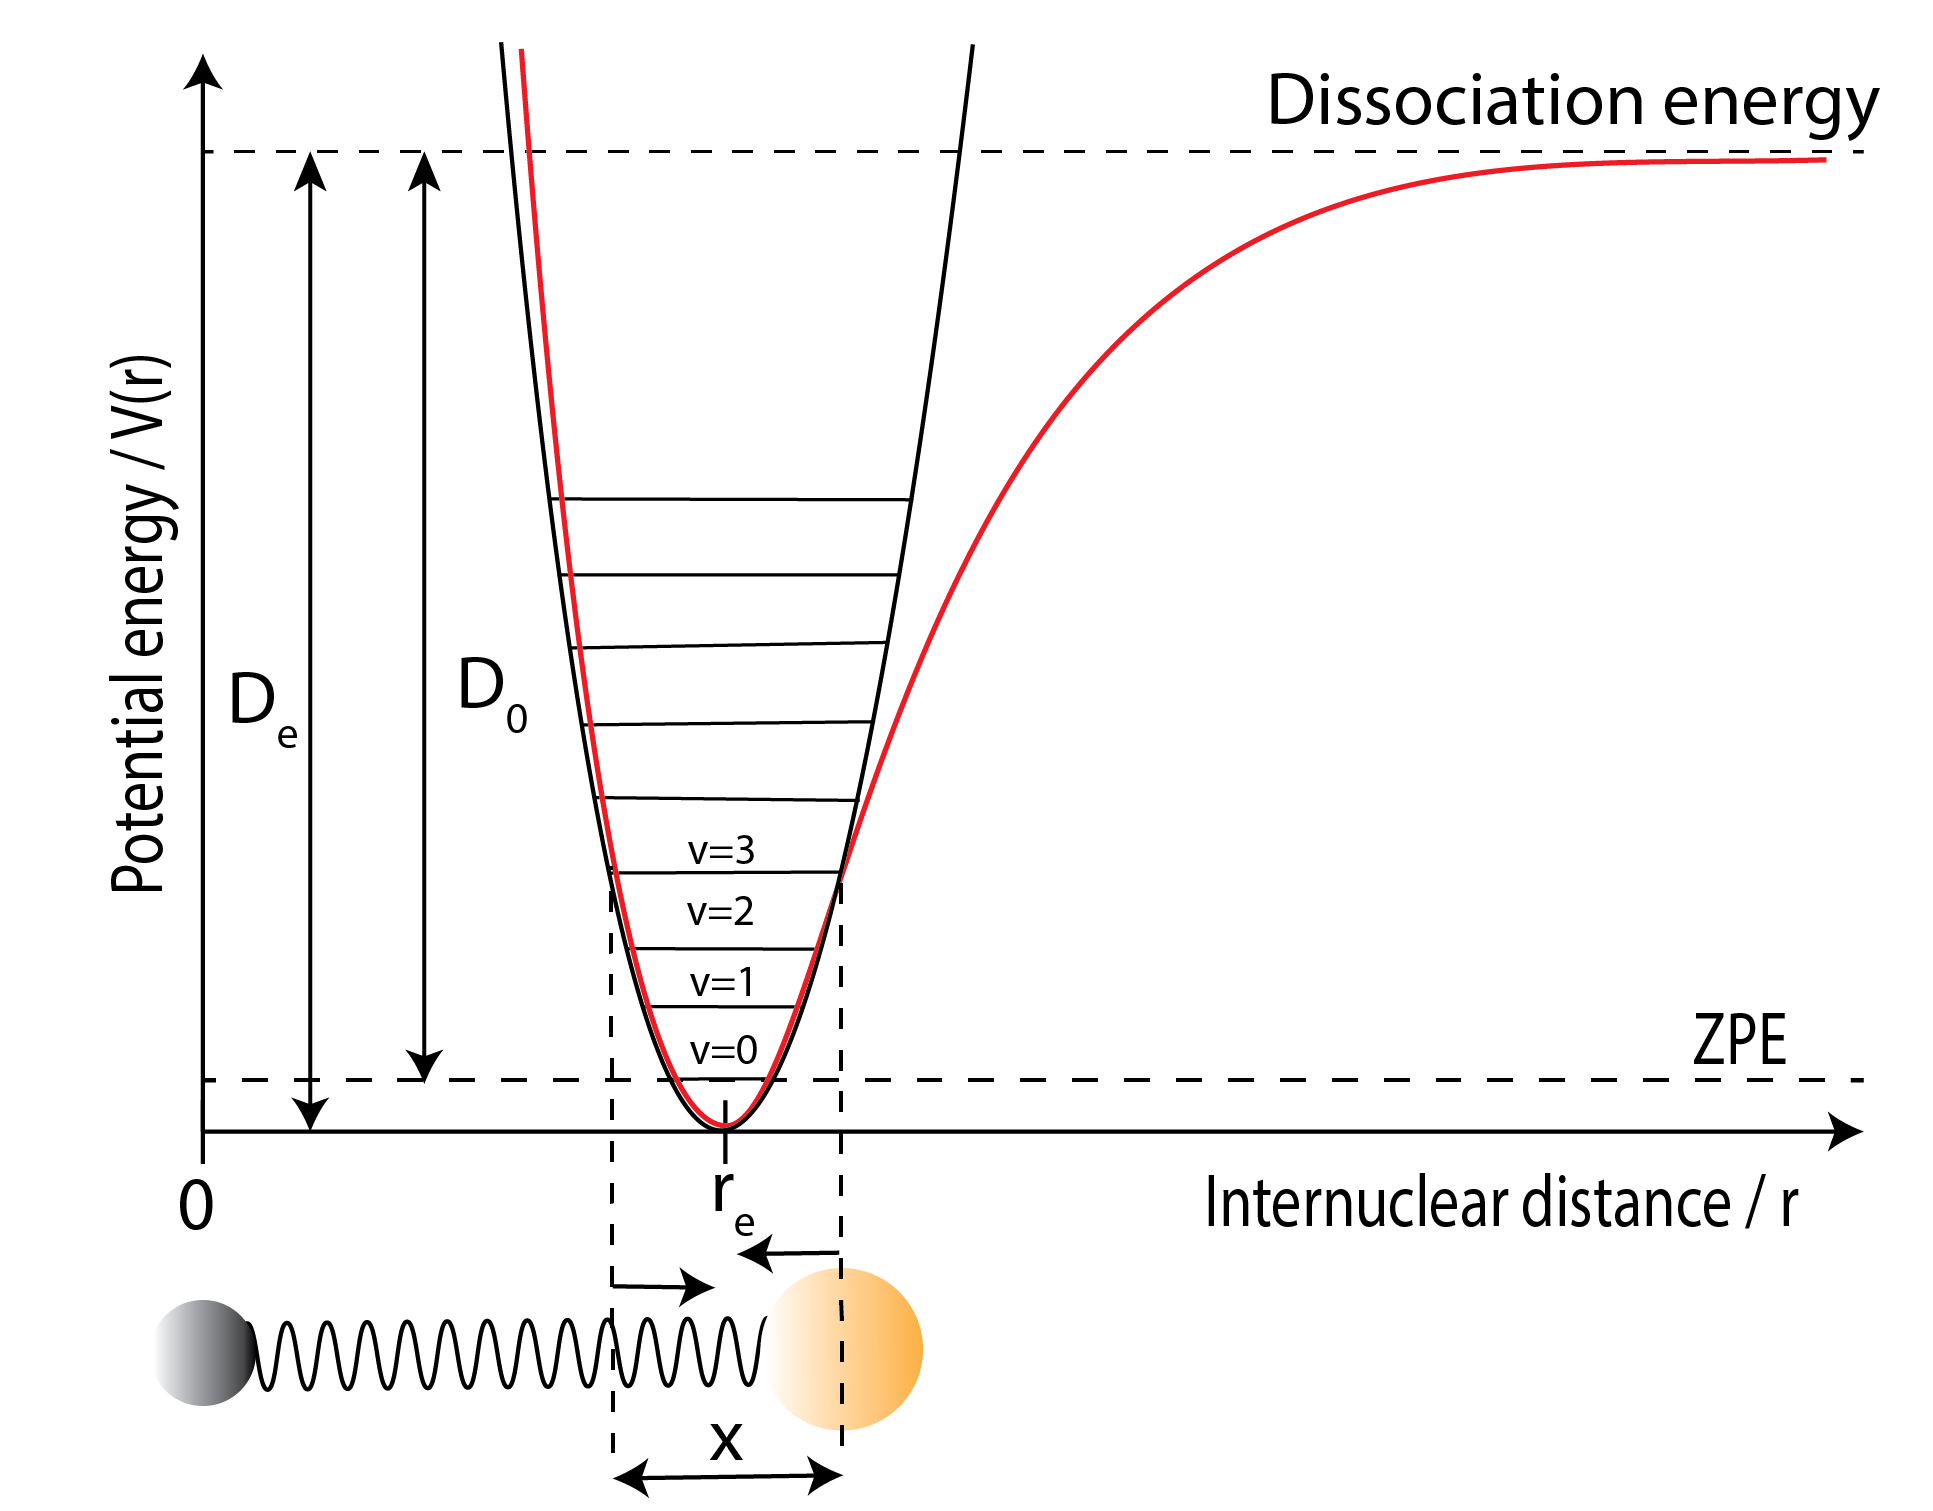
\includegraphics[scale=0.5]{figures/methods/harmonic-oscillator-01.png}
    \caption{Heteronuclear diatomic molecule (solid circles at the bottom) vibrating at energy level $v=3$. The black and red curve represent harmonic and anharmonic (Morse) potential energy curves, respectively. $r_e$ is the equilibrium bond length, $D_0$ and $D_e$ correspond to dissociation energy with and without ZPE (zero-point energy) correction, respectively. }
    \label{fig:vibration:oscillator}
\end{figure}

\subsubsection{Diatomic molecules}
\label{sec:mol-vibration:diatomic}

Assuming a simple ball and spring harmonic oscillator model as shown in Figure \ref{fig:vibration:oscillator} gives us the potential energy ($V$) from Hooke's law:
\[\text{Restoring force} = - \frac{dV(x)}{dx} = -kx\]
where $x=r-r_e$ and $k$ is force constant:

\begin{equation}
    \label{eqn:harmonic-oscillator:V(x)}
    V(x) = \frac{1}{2} k x^2
\end{equation}

Substituting, equation \ref{eqn:harmonic-oscillator:V(x)} in equations \ref{eqn:quantum:Hamiltonian} and \ref{eqn:quantum:wave-eqn}, we get the Schr\"odinger equation for 1D-oscillator:

\begin{equation}
    \label{eqn:hamiltonian-harmonic:V(x)}
    \left( -\frac{\hbar^2}{2\mu} \frac{d}{d x^2} + \frac{1}{2} k x^2 \right ) \psi_v(x) = E_v\psi_v(x)
\end{equation}
where $\mu$ is the reduced mass.

Equation \ref{eqn:hamiltonian-harmonic:V(x)} can be solved to obtain $E_v$ as given below:

\begin{equation}
    \label{eqn:vibrational-energy-Ev}
    E_v = \left( v + \frac{1}{2} \right) h \text{v} = \left( v + \frac{1}{2} \right) hc\omega
\end{equation}

where v is classical vibrational frequency, $\text{v}=\frac{1}{2\pi}\enclose{\frac{k}{\mu}}^{1/2}$, $\omega$ is vibrational wavenumber, the vibrational quantum number is $v=0, 1, 2, ...$ .


Equation \ref{eqn:vibrational-energy-Ev} shows that under the harmonic approximation, the vibrational quantum levels are equally spaced by $\hbar\omega$ and the Zero-point energy (ZPE) i.e., $E_v(v=0)=\frac{1}{2}\hbar\omega$. As shown in Figure \ref{fig:vibration:oscillator}, the ZPE is the minimum energy the molecule may have even at absolute zero temperature because of the uncertainty principle.

The energy terms are usually referred to in wavenumbers [\wn], so we can write Eq. \ref{eqn:vibrational-energy-Ev} as:

\begin{equation}
    \label{eqn:Ev-Gv}
    \frac{E_v}{hc} = \omega \enclose{v + \frac{1}{2}} = G(v)
\end{equation}

where $G(v)$ is the vibrational term value in dimensions of wavenumber, \wn.

As shown in Figure \ref{fig:vibration:oscillator}, the Morse $V(r)$ curve, the actual diatomic molecule is not accurately harmonics, especially when $r \gg r_e$. To account for anharmonicity, the harmonic oscillator term value are modified to a power series in $\enclose{v + \frac{1}{2}}$:

\[G(v) = \omega_e \enclose{v + \frac{1}{2}} - \omega_e x_e \enclose{v + \frac{1}{2}}^2 + \omega_e y_e \enclose{v + \frac{1}{2}}^3 + ...\]

where $\omega_e$ is the vibration wavenumber that a classical oscillator would have for an infinitesimal displacement from equilibrium. $\omega_e x_e$, $\omega_e y_e$, ... are the anharmonic constants.

To determine, say $\omega_e$ and $\omega_e x_e$, at least two transition wavenumbers must be obtained such as $G(1)-G(0)=\omega_0$ and $G(2)-G(1)=\omega_1$. The dissociation energy $D_e$ is given approximately (since including only $\omega_e x_e$ anharmonic term) by:
\[D_e \simeq \frac{\omega_e^2}{4\omega_e x_e}\]\\

\subsubsection{Polyatomic molecules}
\label{sec:mol-vibration:polyatomic}
The vibrational modes of an  $N$-atomic molecule are give by $3N-5$ and $3N-6$ normal vibration modes for linear and non-linear configuration, respectively.

Polyatomic vibrational modes are much more complicated to treat theoretically than diatomic. As shown in Figure \ref{fig:oscillator:water}, a simple ball-spring model with 3-atoms (H$_2$O), even if one of the nuclei is given a sudden displacement, the whole system undergoes very complicated vibrational motions (bending and stretching); this is known as Lissajous motion. For H$_2$O, we get $3(3)-6=3$ normal modes of vibrations ($v_1-v_3$). In general, a normal vibration mode is one in which all the nuclei undergo in-phase harmonic motion with the same frequency but typically with different amplitude.
\begin{figure}[!htb]
    \centering
    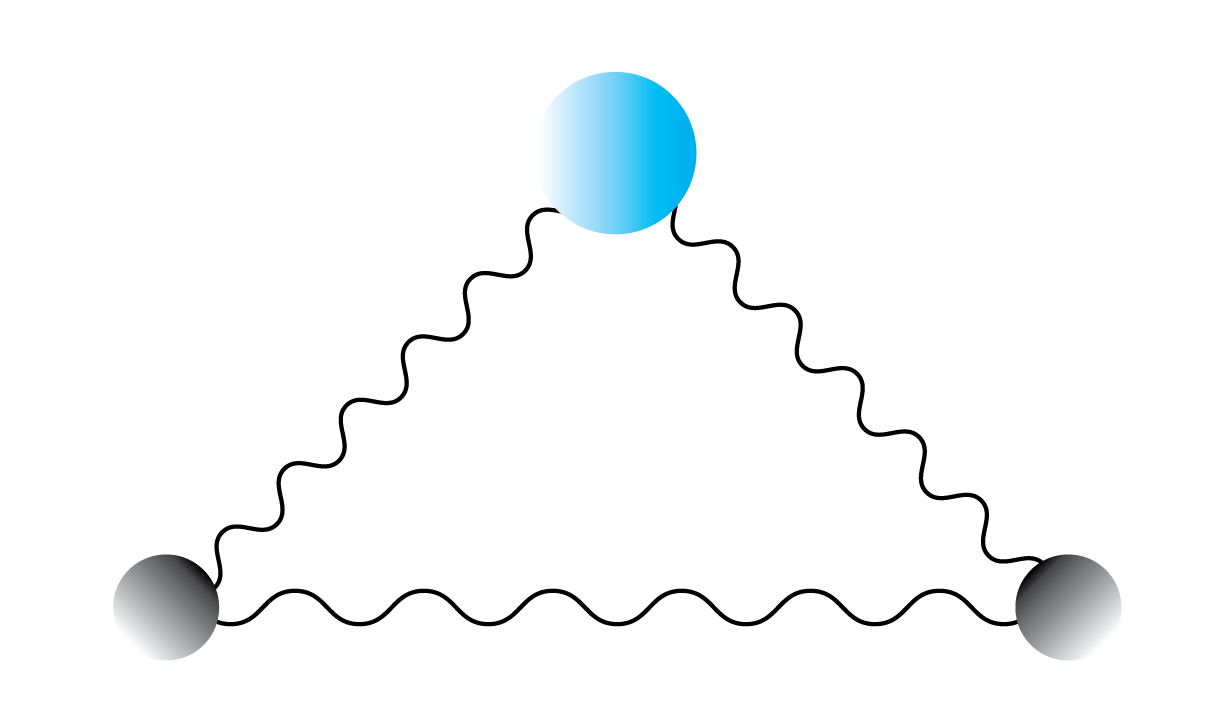
\includegraphics[scale=0.7]{figures/methods/harmonic-oscillator_polyatomic.png}
    \caption{Triatomic molecule (H$_2$O) ball-spring representation. The blue and grey circle represents oxygen and hydrogen, respectively.}
    \label{fig:oscillator:water}
\end{figure}

In polyatomic molecules, each vibrational mode can be approximated to a normal vibrational mode. With an analogous approximation from diatomic, the vibrational term value $G(v_i)$ associated with each normal vibration $i$, is given by:
\[G(v_i) = \omega_i \enclose{v_i + \frac{d_i}{2}}\]

where $d_i$ represents the degree of degeneracy.\\

\subsubsection{Selection rules}
\label{sec:mol-vibration:selection-rule}

When two vibrational states undergo absorption or emission transitions, there is usually an interaction between the molecule and the electric component of electromagnetic radiation. Therefore, the electric dipole moment ($\vec{\mu}$) determines the selection rule for vibrational transitions in the infrared spectrum.

The vibrational transition intensity is proportional to $|R_v|^2$, the square of the vibrational transition moment $R_v$, defined by:

\begin{equation}
    \label{eqn:vib:selctrion-rule}
    R_v = \int \psi^{'} \vec{\mu} \psi{''} d\tau_v
\end{equation}

where $\psi{''}$ and $\psi{'}$ are initial and final vibrational wavefunctions, respectively.\\

A transition is only allowed if the transition dipole integral is non-zero, i.e.:

\begin{align*}
    \begin{split}
        R_v &= 0 \text{ forbidden transition} \\
        R_v &\neq 0 \text{ allowed transition}
    \end{split}
\end{align*}
For diatomic molecules, within the harmonic approximation, $R_v$ is non-zero only when $\Delta v = \pm 1$. Anharmonicity can lead to $\Delta v = \pm 2, \pm 3, ...$, overtone transitions but they are generally weak.

In general, there are simple requirements for the integral of Eq. \ref{eqn:vib:selctrion-rule} to be non-zero; they are as follows.

When both $\psi{''}$ and $\psi{'}$ are non-degenerate, the symmetry species of the quantity to be integrated should be totally symmetric; that is:

\[\Gamma(\psi^{'}) \otimes \Gamma(\vec{\mu}) \otimes \Gamma(\psi^{''}) = A\]

where $A$ denotes the totally symmetric species of any non-degenerate point group, and $\Gamma$ stands for symmetry representation.

For degenerate states:
\[\Gamma(\psi^{'}) \otimes \Gamma(\vec{\mu}) \otimes \Gamma(\psi^{''}) \supset A\]

A brief overview of molecular vibration for diatomic and polyatomic molecules has been discussed, along with the selection rule for observing IR active vibrational transition modes using quantum mechanics. The following section deals with the quantum mechanical theory of molecular rotation.

\subsection{Molecular rotation}
\label{sec:mol-rotation}

Molecules have electronic and vibrational energy due to the motion of electrons and nuclei, respectively. Furthermore, they have rotational energy due to the overall rotation of the molecule. Like electronic and vibrational, rotational energy is quantized and generally has very small energies compared to the former.

\begin{figure}[!htb]
    \centering
    
    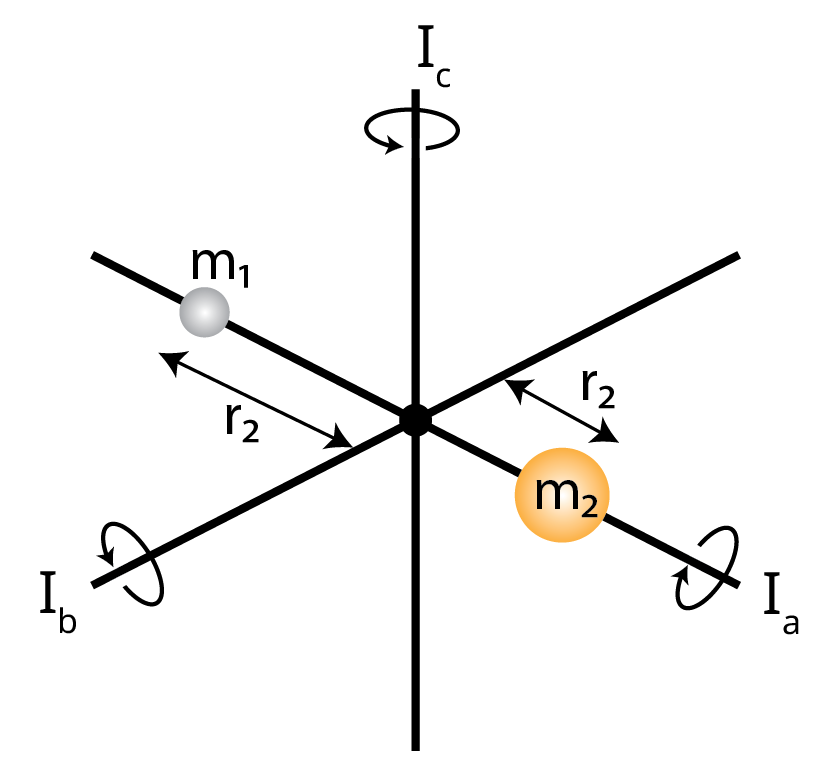
\includegraphics[scale=0.7]{figures/methods/rotation-rotor_linear.png}
    \caption{Rotation of linear molecule (heteronuclear diatomic) w.r.t principal rotational axis $a, b$ and $c$, with corresponding moment of inertia $I_a, I_b$ and $I_c$, respectively ($I_a$=0, $I_b$=$I_c$ for linear and diatomic molecules). $m$ and $r$ represent the mass of the atom and the distance to the rotating axis, respectively. The centre of mass lies at the origin.}
    \label{fig:rotor:diatomic}
\end{figure}

The molecules are classified according to their principal moments of inertia, $I_a, I_b$ and $I_c$, i.e., the moment of inertia along the principal rotational axis $a, b$ and $c$, respectively. The corresponding rotational constants are denoted as $A, B$ and $C$, respectively. The principal axes are perpendicular to each other and pass through the molecule's centre of mass (as shown in Figure \ref{fig:rotor:diatomic}). In general, the axes are conventionally defined such that: 

\begin{equation}
    \label{eqn:Iabc-reltion}
    I_a \leq I_b \leq I_c
\end{equation}

The moment of inertia, $I$, is defined as 

\begin{equation}
    \label{eqn:moment-of-inertia}
    I = \sum_i m_i r_i^2
\end{equation}

where $m_i$ and $r_i$ correspond to mass and distance to the rotating principal axis of atom $i$, respectively.

The main classifications are linear and non-linear molecules, while the latter is further divided, as will be briefly discussed in the following sections.

\subsubsection{Linear molecules}
\label{sec:mol-rotation:linear}

With a rigid rotor approximation, i.e., the bonds are rigid rods and molecule as a rigid rotor, the angular momentum is given by:

\[P_J = [J(J+1)]^{\frac{1}{2}} \hbar\]
where the rotational number $J=0, 1, 2, 3, ...$ .\\

In the presence of an electric or magnetic field,

\begin{equation}
    \label{eqn:rotation:MJ}
    (P_J)_z = M_J \hbar
\end{equation}

where, subscript $z$ represent z-axis component and $M_J = J, J-1, ..., -J$. This indicates that in the absence of an electric or magnetic field, each rotational level has $2J+1$ degenerate states.\\

The rotational energy ($E_r$) for a diatomic or linear polyatomic molecule can be solved using Eq. \ref{eqn:quantum:wave-eqn} and is given by:

\begin{equation}
    \label{eqn:rotational-energy-Er}
    E_r = \frac{h^2}{8\pi^2 I_b} J (J+1)
\end{equation}

The rotational energy in frequencies [Hz] can be defined using Eq. \ref{eqn:rotational-energy-Er}:

\begin{equation}
    \label{eqn:rotational-energy-FJ}
    F(J) = \frac{E_r}{h} = \frac{h}{8\pi^2 I_b} J(J+1) = BJ(J+1)
\end{equation}

where $F(J)$ is the rotational term values and $B$ is the rotational constant.\\
Only $B$ rotational constants are involved for linear molecules since as shown in Figure \ref{fig:rotor:diatomic}, $I_a=0$ and $I_b=I_c$.\\

The rigid rotor approximation does not hold true, especially in higher $J$ energy levels, because the chemical bonds expand due to centrifugal forces from molecular rotation. The expansion due to centrifugal force is included in equation \ref{eqn:rotational-energy-FJ} such that

\begin{equation}
    \label{eqn:rotational-energy-FJ-DJ}
    F(J) = BJ(J+1) -DJ^2(J+1)^2 + ...
\end{equation}

where $D$ is the centrifugal distortion constant. Eq. \ref{eqn:rotational-energy-FJ-DJ} also indicates that further higher-order terms may be included.

\subsubsection{Non-linear molecules}
\label{sec:mol-rotation:non-linear}
The non-linear molecules are further classified based on the principal moment of inertia. Analogous to $B$ rotational constant for linear molecule (Eq. \ref{eqn:rotational-energy-FJ}), the rotational constants $A, B$ and $C$ are given by:

\begin{equation}
    \label{eqn:rotational-constants}
    A=\frac{h}{8\pi^2 I_a};\ B=\frac{h}{8\pi^2 I_b};\ C=\frac{h}{8\pi^2 I_c}
\end{equation}

with units of frequency [Hz].\\

\textbf{Symmetric top: } It has two equal principal moments of inertia which corresponds to two possibilities: (a) $I_a < I_b = I_c$ and (b) $I_a = I_b < I_c$, these are called prolate and oblate, respectively. In symmetric tops, a second rotational quantum number $K=0, 1, 2, ..., J.$ is introduced in addition to $J$; therefore, Eq. \ref{eqn:rotational-energy-FJ} becomes

\begin{align}
    F(J, K) &= BJ(J+1) + (A-B)K^2\ \text{(prolate)} \label{eqn:rotational-energy-FJ-AKJ}\\
    F(J, K) &= BJ(J+1) + (C-B)K^2\ \text{(oblate)} \label{eqn:rotational-energy-FJ-CKJ}
\end{align}

The equations \ref{eqn:rotational-energy-FJ-AKJ} and \ref{eqn:rotational-energy-FJ-CKJ} indicate that for a particular value of $J$, the energy levels diverge and converge for a prolate and oblate symmetric tops, respectively. Since from Eq. \ref{eqn:Iabc-reltion} and \ref{eqn:rotational-constants}, we have $A \geq B \geq C$.\\

When the effect of centrifugal distortion is included, Eq. \ref{eqn:rotational-energy-FJ-AKJ} becomes (for prolate),
\begin{equation}
    \label{eqn:rotational-energy-FJ-KJ}
    F(J, K) = BJ(J+1) + (A-B)K^2 - D_J J^2(J+1)^2 - D_{JK} J(J+1)K^2 - D_K K^4
\end{equation}

where there are now three centrifugal constants $D_J, D_{JK}$ and $D_K$.\\

\textbf{Spherical top: }It has all three principal moments of inertia equal, i.e., $I_a = I_b = I_c$. Therefore, the rotational term value follows the same as the equation for diatomic or linear polyatomic \ref{eqn:rotational-energy-FJ} and \ref{eqn:rotational-energy-FJ-DJ} (Section \ref{sec:mol-rotation:linear}).\\

\textbf{Asymmetric top: } It has all three principal moments of inertia unequal, i.e., $I_a \neq I_b \neq I_c $. Generally, the vast majority of molecules are asymmetric tops. But unfortunately, there are no analytical formulae for rotational term values for asymmetric tops molecules. $J$ is still a good quantum number, but $K$ is not, i.e., it does not take integral values. Therefore, only approximate expressions are derived, i.e., to approximate the molecule to either prolate or oblate near-symmetry top, such as:

\begin{align*}
    \begin{split}
        F(J, K) &\simeq B^* J(J+1) - (A-B^*)K^2\ \text{(near-prolate)} \\
        F(J, K) &\simeq B^* J(J+1) - (C-B^*)K^2\ \text{(near-oblate)}
    \end{split}
\end{align*}

where $B^*$ is equal to $\frac{1}{2} (B+C)$ for prolate and $\frac{1}{2} (A+C)$ for oblate rotor.

Since $K$ is not strictly a good quantum number and the $F(J, K)$ is only approximated.

\subsubsection{Selection rules}
\label{sec:mol-rotation:selection-rule}

Similar to the vibrational selection rule as discussed in Section \ref{sec:mol-vibration:selection-rule}, the rotational selection rule is determined from the rotational transition moment, $R_r$, defined as:

\[R_r = \int \psi_r^{'} \Vec{\mu} \psi^{''}\]

The rotational selection rule constitutes the condition for which $R_r$ is non-zero.\\

The selection rule:\\

for linear molecules and spherical top

\begin{enumerate}
\item $\Delta J = \pm 1$
\end{enumerate}

for symmetric top

\begin{enumerate}
\item $\Delta J = \pm 1$
\item $\Delta K = 0$
\end{enumerate}

for the asymmetric top

\begin{enumerate}
\item $\Delta J = 0, \pm 1$
\end{enumerate}

In addition to the above rules, all molecules must have a permanent electric dipole moment ($\Vec{\mu} \neq 0$) to observe rotational transition, and in the presence of the electric or magnetic field $\Delta M = 0, \pm 1$ (see Eq. \ref{eqn:rotation:MJ}).\\

The next section discusses relevant technical details for quantum chemical calculation employed in this thesis work.

\subsection{Quantum chemical calculations}
\label{sec:QC-calculations}
The molecular vibration and rotation laboratory spectroscopic studies reported in this work are supported by quantum chemical calculations as described in Section \ref{sec:mol-vibration} and \ref{sec:mol-rotation}. This section briefly discusses the methods and programs used to employ quantum chemical calculations.

Initially, a potential energy surface is computed to characterize the molecular ion of interest, and energetically stable structures are derived and structurally optimised. These investigations are performed at the coupled-cluster singles and doubles (CCSD) level augmented by a perturbative treatment of triple excitations, CCSD(T) \cite{raghavachari_fifth-order_1989}, in combination with atomic natural orbital (ANO0, ANO1, and ANO2) basis sets from Alml\"of and Taylor \cite{almlof_general_1987, almlof_atomic_1991} as well as the correlation-consistent valence basis set cc-pVDZ \cite{dunning_gaussian_1989} in the frozen core (fc) approximation. The equilibrium geometries have been calculated using analytic gradient techniques  \cite{watts_open-shell_1992}.

Vibrational modes of molecular ions of interest are further investigated by computing harmonic frequencies using numerical differentiation of gradients \cite{lee_analytic_1991, watts_coupledcluster_1993}. Second-order vibrational perturbation theory (VPT2) \cite{mills_32_1972} has been employed for anharmonic calculations. All CCSD(T) calculations have been carried out using the CFOUR program package  \cite{matthews_coupled-cluster_2020,harding_parallel_2008}.

The influence of the rare gas tag on the IRPD spectrum is further investigated by computing interaction energies (using either CFOUR \cite{matthews_coupled-cluster_2020} or PSI4 \cite{smith_psi4_2020} program) as well as harmonic frequencies of the ionic complexes. For the complexes, the Basis Set Superposition Errors (BSSE) \cite{liu_accurate_1973} are addressed using i) the counter-poise (CP) method introduced by Boys and Bernardi \cite{boys_calculation_1970}, i.e. by calculating CP-corrected CCSD(T) interaction energies at each geometry, and ii) higher-order symmetry-adapted perturbation theory, SAPT2+3 \cite{jeziorski_perturbation_1994, hohenstein_density_2010}. 

Measured pure rotational and vibrational transitions (see Chapter \ref{chapter:CO+}) are fitted with an effective Hamiltonian approach using the Pgopher program \cite{western_pgopher_2017} to derive molecular spectroscopic constants. Further computational details specific to certain ionic species are reported in their respective chapters in detail. The next section focuses on experimental technical details such as determining number density.

\section{Technical details}
\subsection{Determining number density}
\label{subsec:numer-density}

Our experiments produce the target molecular ion of interest at room
temperature. It enters the trap, which is collisionally cooled by a continuous
inflow (for kinetics and ROSAA measurements) of helium buffer gas. This
technique could reach the lowest trap nominal temperature of 4.8(3) K (see
Figure \ref{fig:cooldown_behaviour}). The helium buffer gas pressure is
measured inside the trap using a Spinning Rotor Gauge (MKS SRG3-EL). The SRG
measuring head (SRG-SH700-V3) is mounted outside at room temperature and
connected to the trap via a 3 mm diameter tube. Therefore, thermal
transpiration is considered when calculating the helium number density since
there is a temperature gradient between the trap and the measuring head.\\

\citet{reynolds_xviii_1879} first identified thermal transpiration in 1879. It describes that when a large temperature difference between the two ends of a pipe connecting two vessels filled with a rarefied (low-pressure) gas, a significant pressure difference will be observed between the two ends. Hence, this phenomenon is known as the \textit{thermo-molecular pressure difference effect}. \citet{knudsen_thermischer_1910} in 1910 derived a low-density approximation for this effect, i.e., if the pressure held in the system is so low that the mean free path of gaseous molecules is several times the diameter of the connecting tube, the ratio of the pressure in the respective vessels is then given as:
\begin{equation}
    P_{trap} = P_{SRG} \cdot \sqrt{\frac{T_{trap}}{T_{SRG}}}
    \label{eqn:knudsen}
\end{equation}

where the subscript $trap$ and $SRG$ correspond to the cryogenic ion trap
(low-temperature) and spinning rotor gauge (high-temperature, i.e., room
temperature). They are defined in more detail in the next section. Thus, in
this section, a detailed relationship between the two systems will be
established.\\

The number density in the trap (at low-density approximation), $n_{trap}$, is
given by using the ideal gas law:

\begin{equation}
    n_{trap} = \frac{1}{k_B} \cdot \frac{P_{trap}}{T_{trap}}
    \label{eqn:ideal-gas-law}
\end{equation}

where $k_B$ is the Boltzmann constant.\\

Substituting Eq. \ref{eqn:knudsen} in Eq. \ref{eqn:ideal-gas-law} we get:

\begin{equation}
    n_{trap} = \frac{1}{k_B} \cdot \frac{P_{SRG}}{\sqrt{T_{trap} \cdot T_{SRG}}}
    \label{eqn:number-density-general}
\end{equation}

Substituting $T_{SRG} = 300$ K (room temperature) in Eq.
\ref{eqn:number-density-general}, the number density in \percc\ is given by:

\begin{equation}
    n_{trap} [\text{cm}^{-3}] = 4.18 \cdot 10^{17} \cdot \frac{P_{SRG}[\text{mbar}]}{\sqrt{T_{trap}[\text{K}]}}
    \label{eqn:number-density-lowP}
\end{equation}

At higher pressure, thermal transpiration (TT) correction using Takaishi-Sensui
\cite{Takaishi1963} equation is used:

\begin{equation}
    \left( P_{trap} \right) _{TT} = P_{SRG} \cdot
    \left(1 + \frac
    {\sqrt{\frac{T_{trap}}{T_{SRG}}} - 1}
    {A \cdot X^2 + B \cdot X + C  \cdot \sqrt{X} + 1}
    \right)
    \label{eqn:TakaishiSensui}
\end{equation}

\begin{equation}
    X[\text{mm} \cdot \text{Pa} \cdot \text{K}^{-1}] = \frac{2 \cdot d \cdot P_{SRG} }{T_{trap} + T_{SRG}}
\end{equation}

where $d$ is the connecting tube diameter in mm (3 mm) and pressure is
expressed in Pascal (1 mBar = 100 Pa). \citet{sanderson_ion_1995} empirically
fitted and derived the A, B and C constants in Eq. \ref{eqn:TakaishiSensui} for
helium gas at low temperature (4.35 K)

\[ A [\text{K}^{2}\ \text{mm}^{-2}\ \text{Pa}^{-2}] = 6.11 \]
\[ B [\text{K}\ \text{mm}^{-1}\ \text{Pa}^{-1}] = 4.26 \]
\[ C [\text{K}^{\frac{1}{2}}\ \text{mm}^{-\frac{1}{2}}\ \text{Pa}^{-\frac{1}{2}}] = 0.52 \]

The trap number density including thermal transpiration correction, $\left(
    n_{trap}\right) _{TT}$, is derived by substituting equation
\ref{eqn:TakaishiSensui} in \ref{eqn:ideal-gas-law} and we then get:

\begin{equation}
    \left( n_{trap}\right) _{TT} =
    \frac{1}{k_B} \cdot
    \frac{ \left( P_{trap} \right) _{TT} }{T_{trap}}
    \label{eqn:number-density-highP}
\end{equation}

% \begin{figure}[!htb]
    \centering
    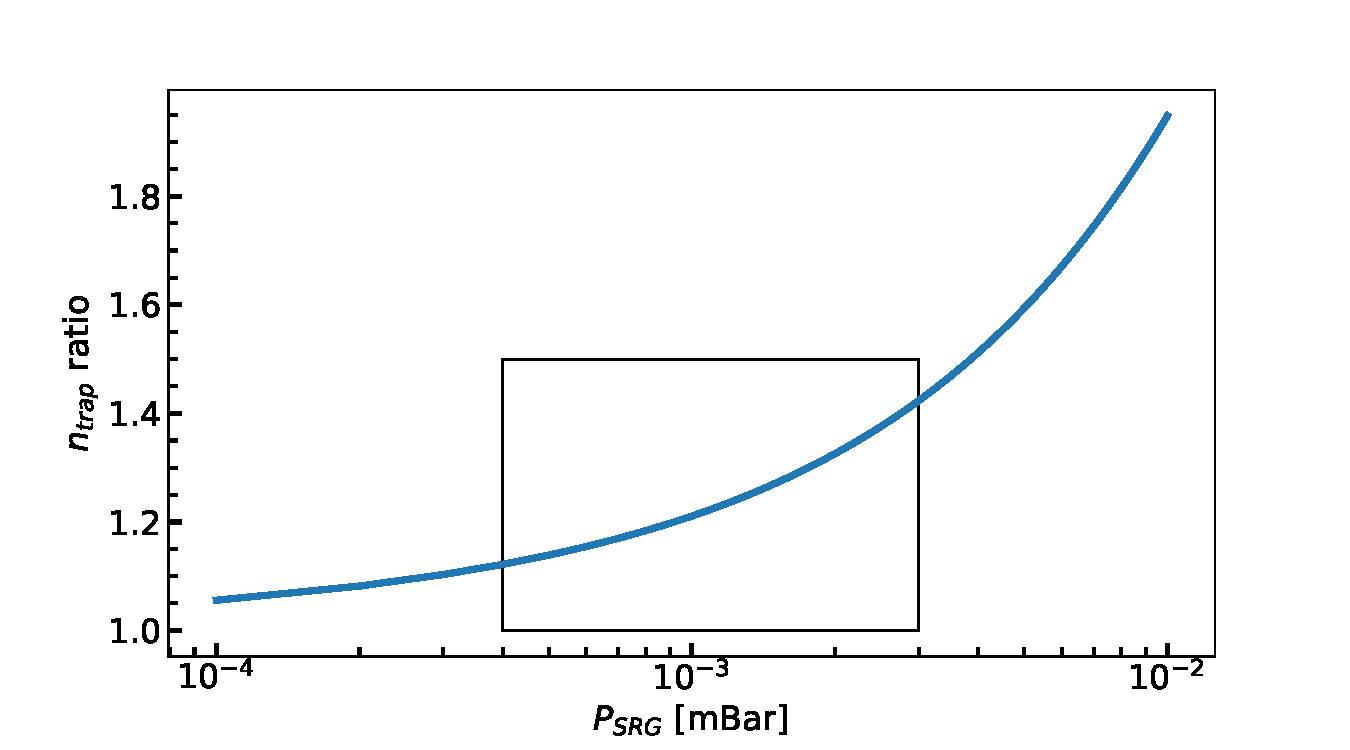
\includegraphics[width=1\textwidth]{figures/measurements/kinetics/numberDensity_ratio.pdf}
    \caption{Comparing number density, $n_{trap}$, with and without thermal transpiration. The figure shows pressure measured using SRG vs $n_{trap}$(Thermal transpiration / low-pressure approximation) ratio. The marked box region indicates the pressure range used in this study.}
    \label{fig:number-density-compare}

\end{figure}
\begin{figure}[!htb]
    \centering
    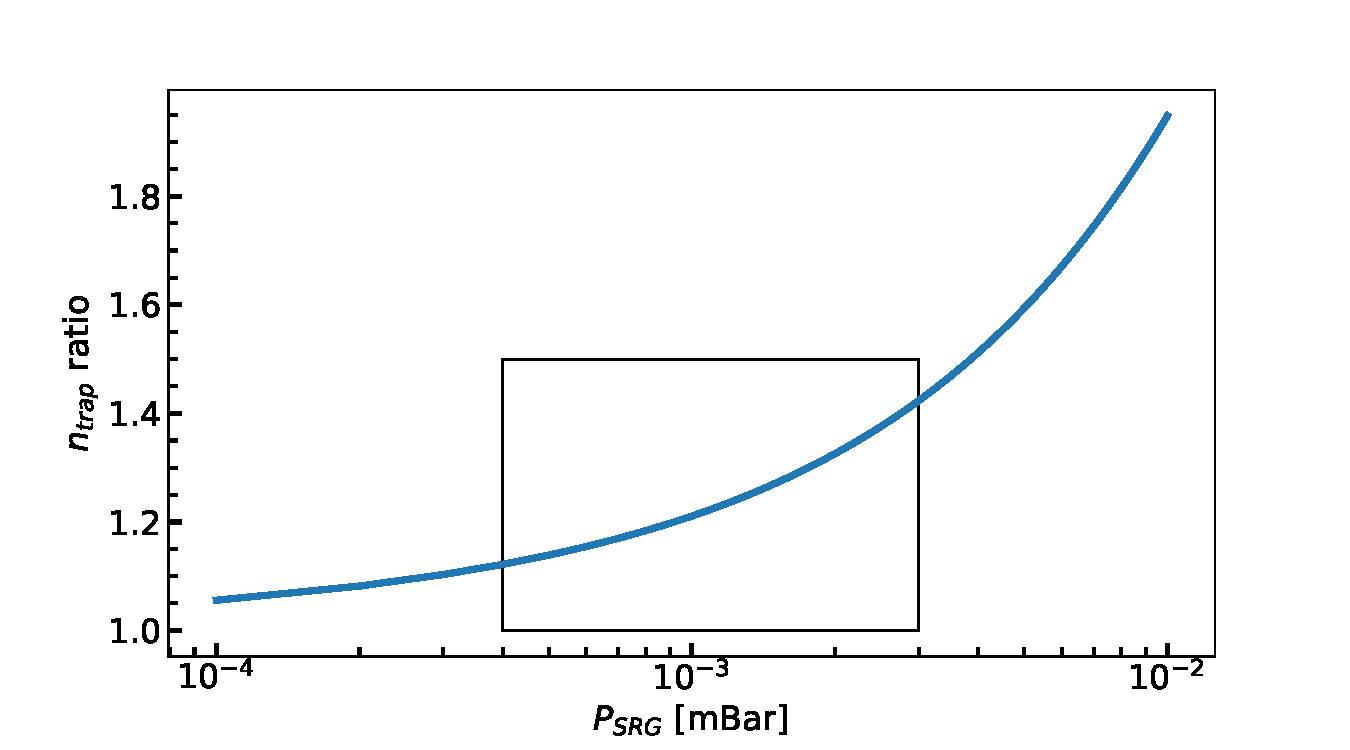
\includegraphics[width=1\textwidth]{figures/measurements/kinetics/numberDensity_ratio.pdf}
    \caption{Comparing number density, $n_{trap}$, with and without thermal transpiration. The figure shows pressure measured using SRG vs $n_{trap}$(Thermal transpiration / low-pressure approximation) ratio. The marked box region indicates the pressure range used in this study.}
    \label{fig:number-density-compare}
\end{figure}

\textbf{Uncertainty considerations:} The computed number density ratio, $n_{trap}$ ratio $= \frac{\left( n_{trap}\right) _{TT}}{n_{trap}}$, is shown in Figure \ref{fig:number-density-compare}. In this thesis work, the number density is determined using thermal transpiration corrections. The pressure is measured using a spinning rotor gauge (SRG), a mean value from 10 iterations per cycle of measurements is taken, and background corrected. When changing the pressure value, a typical wait time of $\sim 5$ min is considered for the system to reach equilibrium. The SRG determines the pressure by measuring the relative rate of deceleration of a metal sphere freely rotating in a vacuum ambience. Therefore, a measurement uncertainty of up to $10 \%$ \footnote{\url{https://www.npl.washington.edu/TRIMS/sites/sand.npl.washington.edu.TRIMS/files/manuals-documentation/MKS-SRG-3-manual.pdf}} must be considered, caused by an increased heating up of the rotor and gas due to the continuous repetition of the sphere drive. In addition,  the room temperature, $T_{SRG}=300 (1)$ K and tube diameter, $d=3.0(1)$ mm. The number density uncertainty is computed through linear error propagation theory using python \textit{uncertainties package} \cite{lebigot_uncertainties_nodate}.

\subsection{Calibration of the hot-cathode ionization gauge (HIG) to SRG}
\label{subsec:calibration:HIG-SRG}

The 22-pole ion trap in the FELion instrument is located at the main chamber
where the temperature $(T_{chamber})$ and pressure $(P_{chamber})$ are
different from the trap $(T_{trap}, P_{chamber})$, because only the trap is
mounted onto the cold head as described in Section
\ref{subsec:setup:ion-trap-and-detector}, and, more importantly, the gas is
admitted into the trap and pumped through the entrance and exit electrodes,
leading to a differential pumping. A schematic diagram of this setup is shown
in Figure \ref{fig:HIG}. As discussed in Section \ref{subsec:numer-density} the
pressure in the trap is measured using a spinning rotor gauge (SRG), i.e.,
$P_{SRG}$. However, the main chamber is also equipped with a hot-ionisation
gauge (Bayard-Alpert gauge, AML AlG17G with NGC2 controller), which is often
used to measure the gas pressure let into the trap. Now, to determine the
number density from the chamber pressure, a relation between $P_{chamber}$ and
$P_{SRG}$ needs to be established and then the number density of gases can be
derived as shown in Section \ref{subsec:numer-density}.\\

\begin{figure}[!htb]
    \centering
    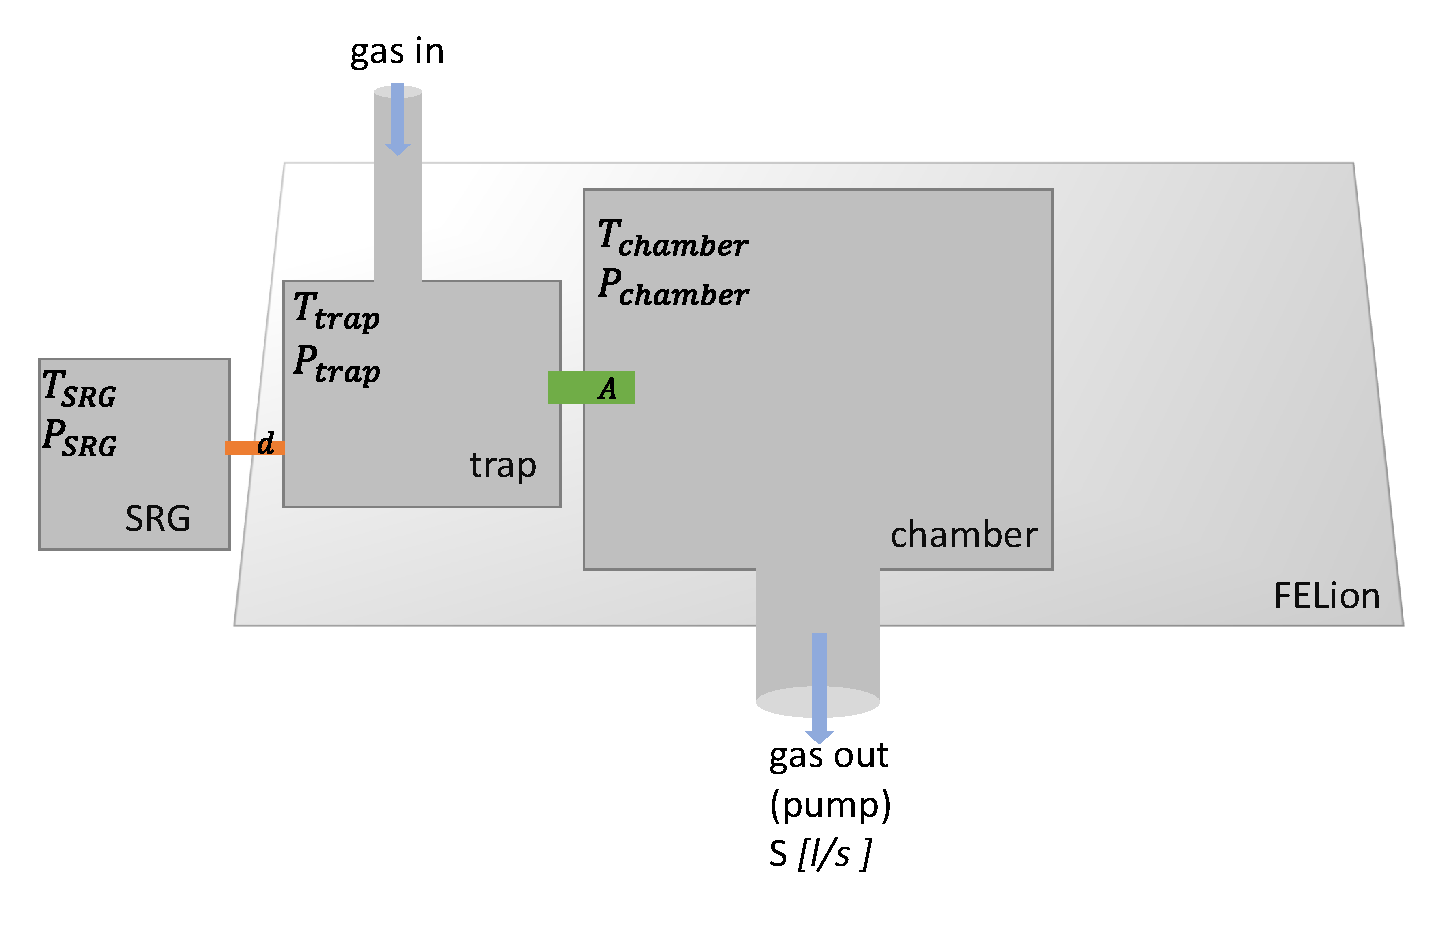
\includegraphics[scale=0.5]{figures/Instruments/HIG calibration.pdf}
    \caption{Schematic diagram on the relation of ion-trap, spinning rotor gauge (SRG) and the main chamber. The orange and green coloured region represents the connecting tube for SRG to trap and trap to the chamber, respectively, with the corresponding aperture of diameter $d$ and $A$.}
    \label{fig:HIG}
\end{figure}

\begin{figure}[!htb]
    \centering
    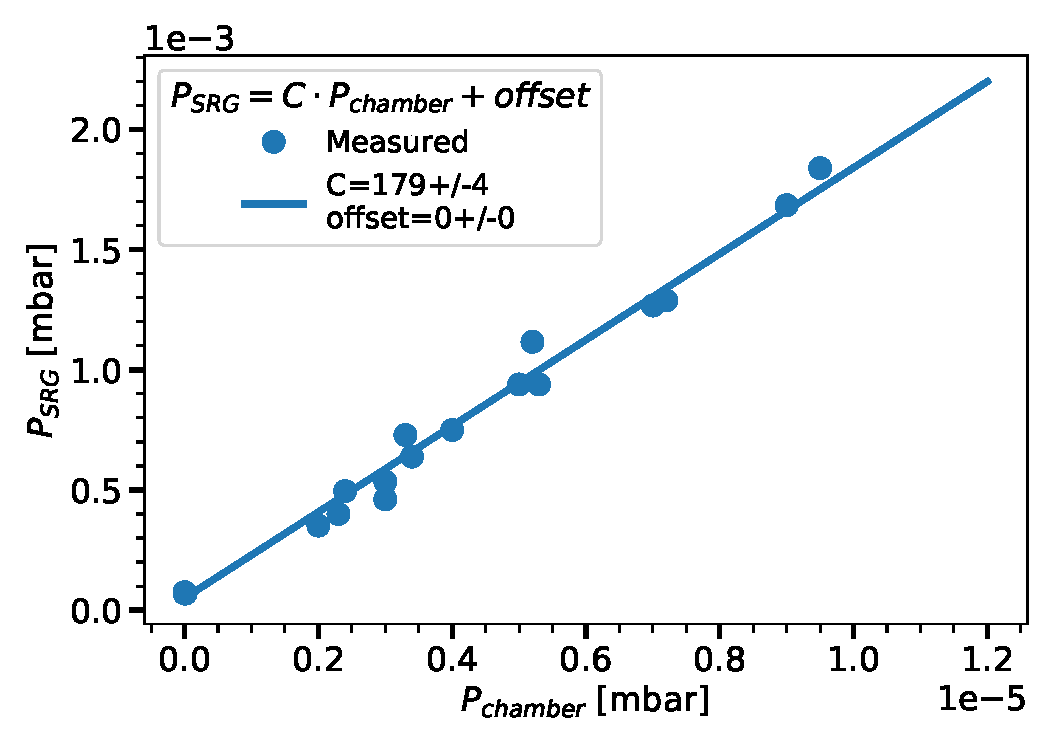
\includegraphics[scale=0.5]{figures/Instruments/SRG_calibration_5K.pdf}
    \caption{Pressure measured with SRG and HIG are plotted at 5 K trap nominal temperature. The derived calibration factor is $C=179(4)$.}
    \label{fig:srg-calibration-5K}
\end{figure}

\textbf{Hot Ionisation Gauge (HIG) background:} In the HIG, electrons are thermionically emitted from a hot cathode filament and  are accelerated into an ionization volume (anode) known as the grid (in the main chamber of our instrument). Collisions between free electrons and neutral buffer gas molecules within the volume may result in ionizing the gas molecule (positive ions), which are accelerated into the ion collector (electrode). The generated positive ion collector current ($i_c$) is directly proportional to the number density of gas, i.e., $P_{chamber}$ as follows

\[ i_c = K \cdot i_e \cdot P_{chamber} \]

where $i_e$ and $K$ are electron emission current and gauge sensitivity,
respectively.\\

\textbf{Pumping speed (S) and throughput (Q):} The throughput of the gas molecule (Q) can be defined in terms of pumping speed, S [liters/s or $l/s$]  and pressure ($P$) as follows
\[ Q = P \ [\text{mbar}] \cdot  S\ [l/s] \]

As shown in Figure \ref{fig:HIG}, the gas is let into the trap (gas in) and
flows into the chamber region with an aperture diameter, A, corresponding to
the two entrance and exit lenses (6 mm diameter each). The speed at which the
gas molecule flows from trap to chamber will depend on the pressure difference
between the two regions as well as the geometry of the chamber in-between,
i.e., aperture ($A$). The factor which accounts for this difference is known as
"conductance" $(C')$, which is defined as

\[ C'_{trap} = \frac{Q_{trap}}{P_{trap} - P_{chamber}}\]

such that,

\begin{equation}
    Q_{trap} = C'_{trap} \cdot (P_{trap} - P_{chamber})
    \label{eqn:throughput-trap}
\end{equation}

If we define the pumping speed ($S_A$) for gas flow from the trap to the
chamber via the aperture of diameter A and $S$ for the pumping speed at which
the gas molecules leave out off the chamber via a vacuum pump (see Figure
\ref{fig:HIG}), then at equilibrium, we get
\begin{equation}
    Q_{trap} = Q_{pump} \Leftrightarrow P_{trap} \cdot S_A = P_{chamber} \cdot S
    \label{eqn:throughput-equilibrium}
\end{equation}

Substituting Eq. \ref{eqn:throughput-trap} in \ref{eqn:throughput-equilibrium},
we get

\[ C'_{trap} \cdot (P_{trap} - P_{chamber}) = P_{chamber} \cdot S \]
which becomes,

\begin{equation}
    \frac{P_{trap}}{P_{chamber}} = 1 + \frac{S}{C'_{trap}} = C
    \label{eqn:trap-chamber-final}
\end{equation}

where $C$ is the calibration factor for pressure between the trap and the
chamber. \\

Since we are measuring the trap pressure using SRG, i.e., $P_{trap}=P_{SRG}$
and the SRG temperature is the same as the chamber (both at room temperature,
$RT$), i.e., $T_{SRG}=T_{chamber}=RT$, from equation
\ref{eqn:trap-chamber-final}, we get

\begin{equation}
    P_{SRG} = C \cdot P_{chamber}
    \label{eqn:srg-chamber-final}
\end{equation}

The above equation \ref{eqn:srg-chamber-final} provides us with the required
relation between SRG and HIG pressure measurement. Figure
\ref{fig:srg-calibration-5K} shows the derived calibration value at 5 K trap
nominal temperature, i.e., $C=179(4)$ at 5 K. The $C$ value is also found to be
temperature independent but depends only on the settings for HIG (the
sensitivity is set to N$_2$ gas).

\part{Vibrational spectroscopy}
\chapter{Laboratory gas-phase vibrational spectra of \texorpdfstring{[C$_3$H$_3$]$^+ $}\ isomers and isotopologues by IRPD spectroscopy}\label{chapter:C3H3+}
\chaptermark{Vibrational spectra of \texorpdfstring{[C$_3$H$_3$]$^+ $}\ isomers}

% \begin{center}
%     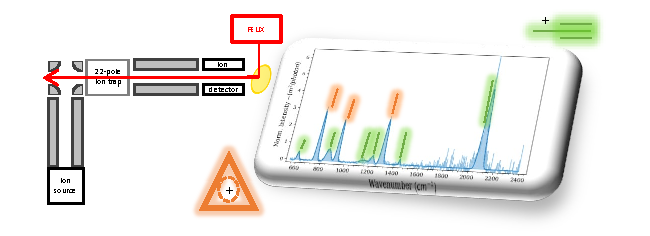
\includegraphics[width=1\textwidth]{chapters/C3H3+ and C3D3+/figures/gabstract.pdf}
% \end{center}

\blfootnote{This chapter is adapted from: Marimuthu, A. N.; Sundelin, D.; Thorwirth, S.; Redlich, B.; Geppert, W. D.; Brünken, S. Journal of Molecular Spectroscopy 2020, 374, 111377
}
\newcommand{\iso}{[C$_3$H$_3$]$^+$ }
\newcommand{\isoD}{[C$_3$D$_3$]$^+$ }
\newcommand{\cyc}{c-C$_3$H$_3^+$ }
\newcommand{\cycD}{c-C$_3$D$_3^+$ }
\newcommand{\lin}{H$_2$C$_3$H$^+$ }
\newcommand{\linD}{D$_2$C$_3$D$^+$ }
\newcommand{\ison}{[C$_3$H$_3$]$^+$}
\newcommand{\isoDn}{[C$_3$D$_3$]$^+$}
\newcommand{\cycn}{c-C$_3$H$_3^+$}
\newcommand{\cycDn}{c-C$_3$D$_3^+$}
\newcommand{\linn}{H$_2$C$_3$H$^+$}
\newcommand{\linDn}{D$_2$C$_3$D$^+$}

\section*{Abstract}
Gas phase vibrational spectra of \iso isomers and their fully deuterated isotopologues 
measured in a cryogenic 22-pole ion trap are presented. The widely tunable free electron 
laser for infrared experiments, FELIX, was employed to cover the frequency range 
500-2400~\wn, complemented with an OPO/OPA system covering 2800-3400~\wn. 
Spectral assignments for both the linear and cyclic isomeric form 
(\lin and \cycn, respectively) are made based on various high-level 
computational studies. The effect of ion source conditions and 
different precursors (allene and propargyl chloride) for the preferential 
production of a specific isomer is discussed. 
The perturbation of the vibrational band position due to complexation with Neon in the recorded infrared-predissociation (IRPD) spectra are also reported in this study.
\clearpage

\section{Introduction}
Hydrocarbon ions with the chemical composition \iso are important intermediates in combustion processes, where they initiate soot formation \citep{Goodings1979,Wheeler2007,Miller2005}, and in various astrochemical environments such as the interstellar medium (ISM) \citep{Herbst1983,Adams1987,CGG1991,smith_ion_1992}, cometary surfaces \citep{korth_probable_1989}, and planetary atmospheres \citep{Anicich2000,Ali2013}. The ion has two stable isomers, the cyclic cyclopropenyl cation, \cycn, and the linear propargyl cation, \linn, see Figure \ref{FIG:C3H3+:molecule}. The \cyc isomer is lower in energy by 28~kcal/mol \citep{HTL2011}, and a significant activation barrier of about 50~kcal/mol separates the two isomers \citep{Duncan2012}. \cyc is the smallest aromatic cation stabilised by two delocalised $\pi$ electrons; hence it has been observed as a common stable fragment from the electron impact ionization mass spectra of many larger hydrocarbon molecules \citep{baer_ng_powis_1996,holmes_aubry_mayer_2007}.\\

In the interstellar medium, \iso is formed by radiative association addition of H$_2$ to linear C$_3$H$^+$, a molecular ion recently detected in several astronomical sources \citep{PGG2012,MCL2013,MCS2014} based on accurate laboratory spectroscopic determination of its rotational spectrum \citep{brunken_laboratory_2014,MCM2015}. Experimental and theoretical studies support the formation of both isomeric variants of \iso in this process \citep{SA1987,Adams1987,MMY1993}. Both \cyc and \lin  are assumed to be the major precursors (via dissociative recombination) of cyclic and linear forms of [C$_{3}$H$_{2}$] and [C$_3$H] \citep{Herbst1983, Adams1987, smith_ion_1992}, which are ubiquitous molecules in the interstellar medium \citep{Thaddeus1985,MI1985,CGG1991,KKO1991,CCF1999,YSO1987,TGH1985}. The observed large variation in the cyclic-to-linear isomeric ratio of both neutrals across different astronomical sources is intricately linked to the formation and destruction of isomeric variants of \iso \citep{MMH1993,CGP2015,SSC2016,LAW2017}. Apart from the main isotopologues, also singly and even doubly deuterated variants of [C$_{3}$H$_{2}$] were detected \citep{BFM1986,SBS2013,SGB2016}, and are frequently used to investigate deuterium fractionation via gas-phase processes in cold dark clouds \citep{GWC1987,BAM1988,MGA2017}. Although many details about the exact deuteration mechanisms are only partly understood, they all involve deuterated variants of \iso \citep{SSG2005,SBS2013}. It should also be noted that due to its D$_{3h}$ symmetry, the \cyc isomer has no pure rotational spectrum, thus its direct observation is not possible by radio-astronomy. However, the linear isomer \lin  and also singly or doubly D-substituted variants of \cyc possess a permanent dipole moment, and are therefore good candidates for radio-astronomical detection. \\  


In a recent study of Titan`s atmosphere by the Ion and Neutral Mass Spectrometer (INMS) onboard the CASSINI spacecraft, a strong signal at $m/z=39$ corresponding to the \iso cation has been recorded \citep{VYM2007}. Although these mass spectrometric detections do not allow to identify the isomeric composition, one can assume the presence of both \iso isomers \citep{Ali2013}. Reactions of \linn, which was found in experiments to be much more reactive than the aromatic \cyc isomer \citep{SLA1982,MMF1994,Anicich1993}, with unsaturated hydrocarbons could be the first elongation steps leading to larger ions, including polycyclic hydrocarbons, in this environment. Upon dissociative and radiative recombination with electrons, heavy neutrals, i.e. tholins, can be formed. Similar processes could happen in other astronomical objects like dark clouds, circumstellar envelopes, star-forming regions, and protoplanetary disks. Model calculations of chemical networks in those environments are dependent on exact data about the reactivity of all isomers of a certain ion. Therefore, it is important to find pathways to produce the isomers selectively to be able to assess their reactive properties in experimental kinetic studies. This has already been done for other ions showing isomers with different reactivity, e.g. for CH$_2$CN$^+$ \citep[][and references therein]{FGK2016}. Although the results are encouraging, the most reliable way to pin down the identities of isomers produced by a certain method is via spectroscopic methods. \\

Due to their importance in astrochemistry and other fields, numerous experimental and theoretical spectroscopic studies exist on the \iso cations. Breslow and co-workers measured the first infrared spectra of \cycn, but in acid solutions as a stable salt \citep{Breslow1970}. Both isomers were later studied in a Neon matrix by electronic and vibrational spectroscopy \citep{Wyss2001}. Very recently the vibrational spectrum of \lin and its fully deuterated form was measured in Argon matrix \citep{Chin2018}. The first gas-phase vibrational spectra covering the C-H stretching region of \iso were measured using an infrared-predissociation (IRPD) method \citep{Roth2002,DRM2002}, and interpreted through high-level quantum-chemical calculations of the ionic structure including the influence of the various tagging agents \citep{BOR2011,BO2011,Botschwina2011}. The experiments were later extended by Ricks et al., who observed several additional fundamental vibrational bands down to the dissociation limit of the Argon tag that they used in the IRPD experiments (approximately 1000~cm$^{-1}$) \citep{RDS2010}. However, some ambiguity in the assignment of several bands of both isomers remained \citep{HTL2011,Duncan2012}. Linnartz and co-workers reported the first high-resolution gas-phase IR spectra of the fundamental $\nu_{4}$ asymmetric C-H stretching band for free (i.e., without ligand tagged) \cyc using continuous wave cavity ring-down spectroscopy \citep{ZDL2014}, and found excellent agreement of their results to spectroscopic parameters obtained from high-level ab initio calculations of quartic force fields \citep{HTL2011}. Additional information of vibrational band positions of \iso comes from photoelectron studies \citep{GLY2012,GGK2018} and electronic spectroscopy \citep{CSD2015}. \\

In this study we report the broad range (550-3400~cm$^{-1}$) vibrational spectra of gas-phase \iso and its fully deuterated variants using different tagging agents (Ne, H$_2$), ion-sources, and precursors. We employed IRPD action spectroscopy in a cryogenic ion trap coupled to the powerful and widely tunable FELIX free-electron IR lasers. The aim of this study is manyfold: (i) to unambiguously assign the vibrational bands of both isomers by comparison to quantum-chemical calculations, which then, in turn, can be used to benchmark these calculations; (ii) to investigate isomer-selective formation mechanisms as a prerequisite for isomer-specific kinetic studies; (iii) to obtain reliable IR data that can be used to spectroscopically distinguish the isomeric \iso products of ion-molecule reactions, and (iv) to provide a basis for follow-up high-resolution rotational studies of those isomers and their isotopologues that possess a permanent dipole moment to aid their astronomical detection.


\begin{figure}
	\centering
		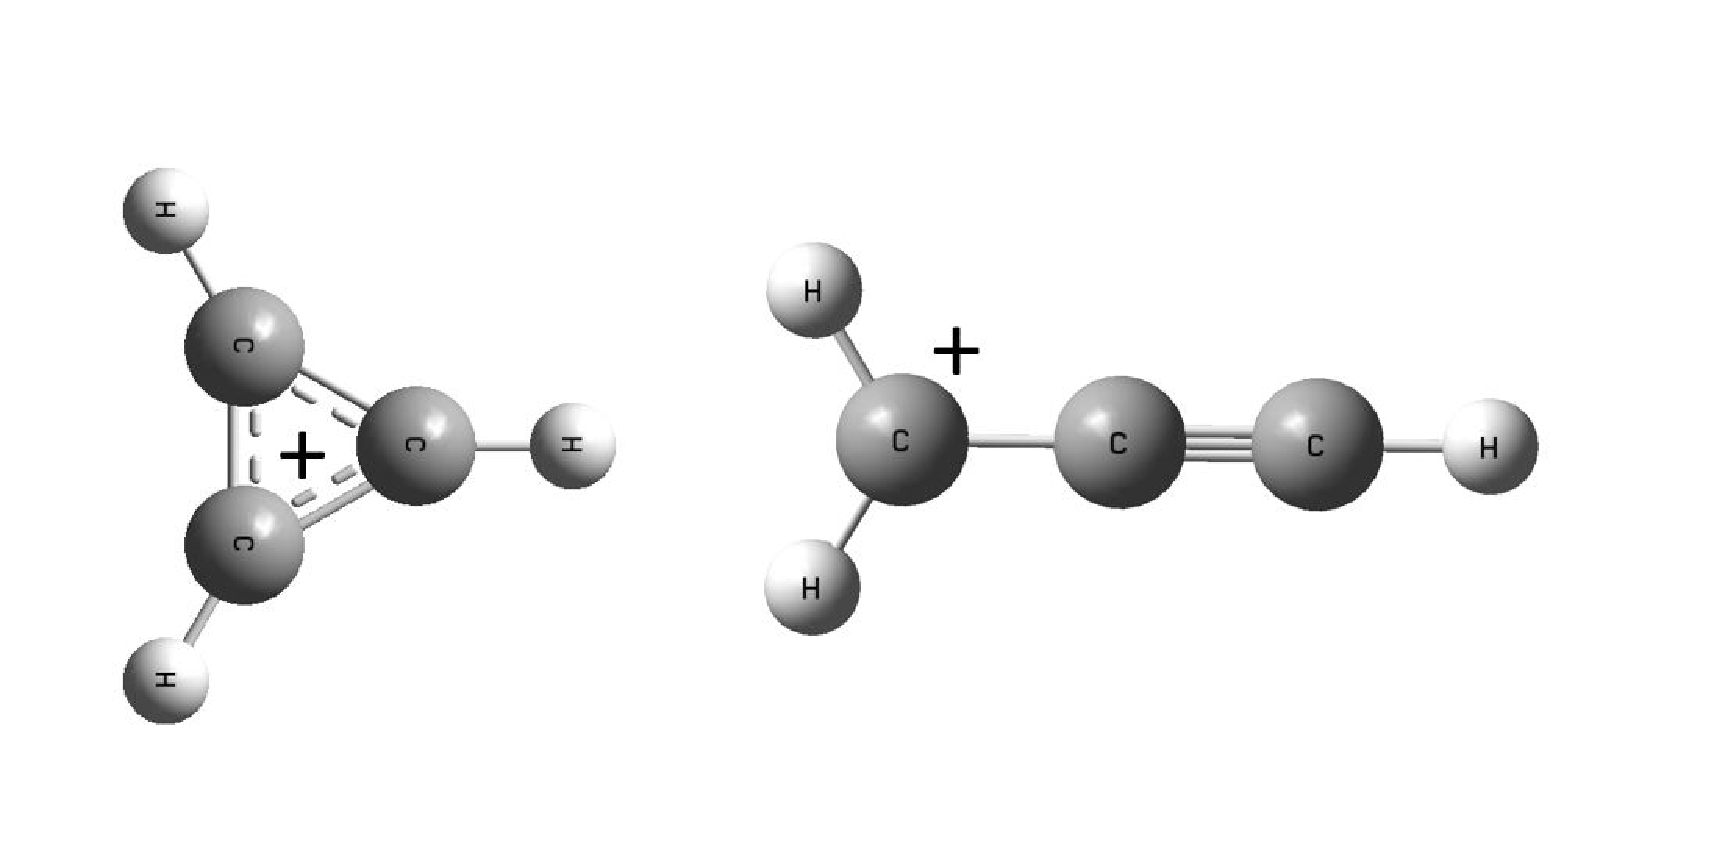
\includegraphics[scale=.4]{chapters/C3H3+ and C3D3+/figures/molecule.pdf}
		\caption{Molecular structures of \cyc (left) and \lin (right) isomers.}
	\label{FIG:C3H3+:molecule}
\end{figure}

\section{Methods}

\subsection{Experimental details}
\vspace{0.5cm}

\begin{figure}

	\centering
		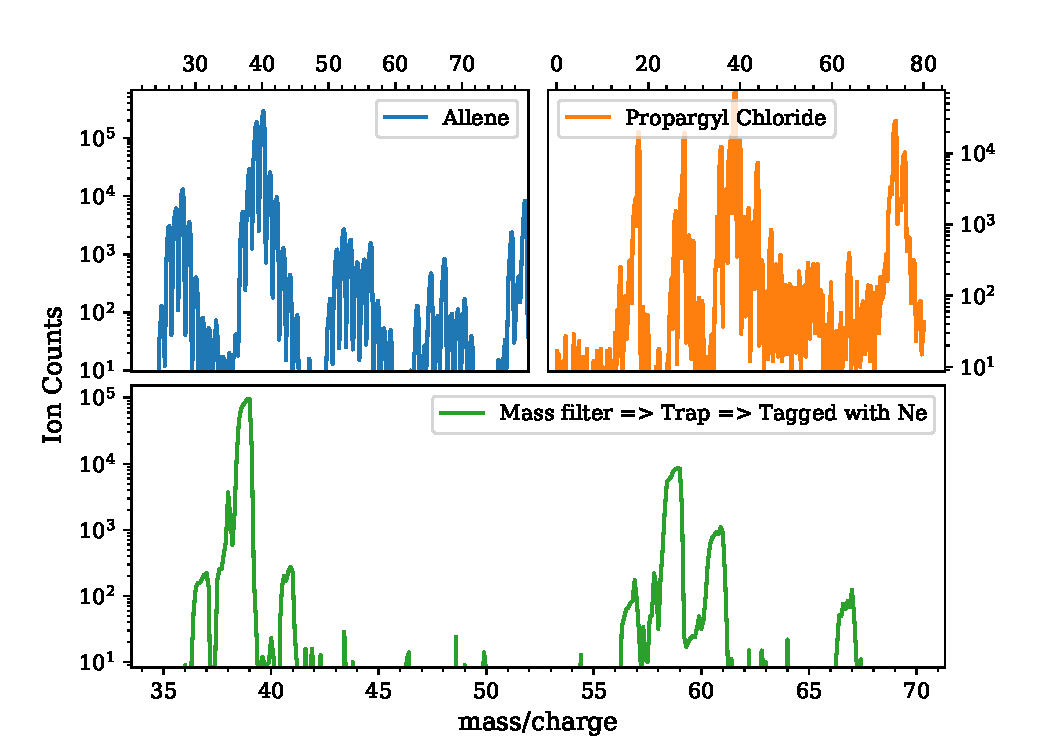
\includegraphics[scale=.7]{chapters/C3H3+ and C3D3+/figures/masspec.pdf}
		
	\caption{Mass spectra of ions produced from electron impact ionization (20~eV) of allene (left, in storage EI source) and propargyl chloride (right, in direct EI source) precursors (upper panel), and of mass filtered \iso (m = 39~u) together with tagged Ne-\iso (m = 59~u) species produced in the cryogenic ion trap (lower panel).}
	
	\label{FIG:C3H3+:masspec}
\end{figure}

The vibrational spectra of the \iso isomers and isotopologues were recorded using the FELion cryogenic 22-pole ion trap instrument located at the Free Electron Lasers for Infrared eXperiments (FELIX) Laboratory (see Section \ref{subsec:ir:radiation-source:FELIX}). A detailed account of the FELion instrument is provided in Section \ref{sec:felion} and the infrared-predissociation (IRPD) of in-situ rare gas tagged cold molecular ions in Section \ref{subsec:action:methods:vibrational:IRPD}. Here we only give a brief account of details specific to the \iso system. \\

Isomeric variants of \iso (m=39~u) were produced by electron impact ionization (electron energy $11-70$~eV) from neutral allene (C$_3$H$_4$, abcr GmbH, 96~\%)  and propargyl chloride (HC$_3$H$_2$Cl, Sigma Aldrich, 98~\%). Fully deuterated [C$_3$D$_3$]$^+$ was produced from deuterated allene (C$_3$D$_4$, Qmx Laboratories, 98~\%). The precursor gases were admitted either pure or diluted with He at a ratio of 1:3 to the ion source chamber at a pressure of $\sim 10^{-5}$~mbar. For most experiments, a simple electron-impact (EI) source was used, and additional measurements were done with a Gerlich-type storage ion source (SIS) \cite{Gerlich1992}, where primary ions produced by EI are accumulated for the duration of an experimental cycle (of the order of seconds), thereby allowing further reactions with the present neutral gas (see Figure \ref{FIG:C3H3+:masspec}).\\

For spectroscopic experiments a few 10~ms long pulse of ions is extracted from the respective source and filtered for the mass of interest, m=39~u in the case of \iso and m=42~u for [C$_3$D$_3$]$^+$, by a quadrupole mass selector before entering the 22-pole ion trap which is held at a fixed temperature in the range 6.1-7~K for experiments using Ne and 11~K for those using H$_2$ as tagging gasses. Around 10-20~ms before the ions enter the trap, an intense 80-150~ms long Ne:He (or H$_2$:He) pulse (1:3 mixing ratio and number density of $\sim 10^{15}$~cm$^{-3}$) is admitted to the trap, leading to efficient collisional cooling of the ions to the ambient temperature. Under these conditions, several 10~\% of the primary ions form weakly bound complexes with Ne (or H$_2$), see Figure \ref{FIG:C3H3+:masspec}. The ions are stored for several seconds in the ion trap and are exposed to several laser pulses before extraction. An IRPD spectrum is recorded by mass-selecting and detecting the \ison-Ne(H$_2$) complex ions while tuning the laser frequency $\nu$. A relative depletion $D=1-\frac{N_{ON}(\nu)}{N_{OFF}}$ in the number of complex ions $N_{ON}(\nu)$ from the baseline value $N_{OFF}$ is observed upon resonant vibrational excitation. To account for varying laser pulse energy $P$, pulse number $n$, and for saturation effects, the signal is normalized prior to averaging using $I=\frac{- ln(N_{ON}(\nu)/N_{OFF})}{n\cdot P/(h\nu)}$, giving the intensity $I$ in units of relative cross-section per photon\footnote{This equation only holds for isomer-pure ionic samples. Saturation effects in isomeric mixtures are underestimated in this way, leading to varying intensity ratios in the presented spectra.}. After normalizing each measurement in this way, the final spectrum is then obtained by averaging using statistical binning with a typical bin size of 2.5~\wn. Line parameters such as band positions, intensities, and line widths (fwhm) are then obtained by fitting a multi-component Gaussian function to the experimental data, also providing statistical errors of the line parameters. \\

Additionally, we performed saturation depletion experiments (see section \ref{iso}) to quantify the isomeric ratio of the ionic mixture as described in detail previously \citep{JSB2018,jusko_felion_2019}. Here we used up to 46 laser pulses, resonant with an isomer-specific vibrational band position, to fully deplete (dissociate) just one isomer complex. The analysis of the depletion signal as a function of laser pulses, corrected for other loss-mechanisms, allows then to derive both the absorption-dissociation cross-section and the isomer abundance. \\

The vibrational IRPD spectra were recorded using the IR radiation of FEL-2 of the FELIX Laboratory in the frequency region 550-2400 cm$^{-1}$, also employing the 3rd harmonic mode of the FEL. The laser was operated at 5 or 10~Hz with macro pulse energies in the interaction region between 1.5-60~mJ, and for each datapoint $n=$3-66 pulses were admitted depending on the signal strength. The FEL was optimized for narrow bandwidth with a full width at half-maximum (fwhm) of $0.3-1$~\% of the center wavelength. Additional spectra were recorded in the C-H-stretching region between 2800-3400~\wn using a Laservision OPO/OPA system ($\sim 3$ \wn\ fwhm, 10 Hz, 5~ns pulses) with typical power of $\sim$ 7-10~mJ.\\



\subsection{Computational details} 
\vspace{0.5cm}

The \iso  system has previously been studied quantum-chemically on several occasions
and at various levels of theory  \citep{HTL2011,BOR2011,BO2011,Botschwina2011}.
In the present investigation of the hydrogenated and perdeuterated variants, quantum chemical calculations have been performed 
at the coupled-cluster singles and doubles (CCSD) level 
augmented by a perturbative treatment of triple excitations, CCSD(T) \cite{raghavachari_chemphyslett_157_479_1989}, 
together with atomic natural orbital (ANO0, ANO1, and ANO2) basis sets from
Alml\"of and Taylor \cite{almlof_JCP_86_4070_1987}. The ANO0, ANO1, and ANO2 basis sets consist of 13s8p6d4f2g to 3s2p1d, 4s3p2d1f, and 5s4p3d2f1fg contractions for C as well as 8s6p4d3f to 2s1p, 4s2p1d, and 4s3p2d1f contractions for H, respectively. Equilibrium geometries have been calculated using analytic gradient techniques
\cite{watts_chemphyslett_200_1-2_1_1992}, while
harmonic frequencies have been computed using analytic second-derivative techniques
\cite{gauss_chemphyslett_276_70_1997,stanton_IntRevPhysChem_19_61_2000}.
For anharmonic calculations, second-order vibrational perturbation theory (VPT2) \cite{mills_alphas}   
has been employed and additional numerical differentiation of analytic second derivatives has been applied 
to obtain the third and fourth derivatives required for the application of VPT2  \cite{stanton_IntRevPhysChem_19_61_2000,stanton_JCP_108_7190_1998}.
The frozen core approximation has been used throughout.
All calculations (including those employing VPT2) have been carried out using the CFOUR program package \cite{cfour_JCP_2020,harding_parallel_2008}. \\

The CCSD(T) method in combination
with ANO basis sets has been shown previously to provide vibrational wavenumbers of high quality \cite{mccaslin_MolPhys_111_1492_2013,thorwirth_JMS_251_220_2008}.
In the present investigation, harmonic force fields were calculated at the
CCSD(T) /ANO2 level throughout. 
For the \cycD and \lin species, best estimates of the fundamental vibrational wavenumbers
were then calculated by applying anharmonic vibrational corrections 
calculated at the CCSD(T)/ANO1 level to the CCSD(T)/ANO2 harmonic wavenumbers.
Because of numerical problems in the CCSD(T)/ANO1 VPT2 calculation, for the 
\cyc and \linD species, anharmonic corrections were taken from corresponding CCSD(T) /ANO0 calculations. A comparison of the fundamental vibrational frequencies obtained in this fashion
using CCSD(T)/ANO1 and CCSD(T)/ANO0 for the \cycD and \lin species reveals that
the differences between the two levels are small, order of a few cm$^{-1}$ only.
From the anharmonic force field calculations we also find that in the \cycD species,
the $\nu_1$ mode is in resonance with the overtone of the $\nu_5$ mode
(using thresholds of $\Delta \omega = 50$\,cm$^{-1}$ and $\Phi_{ijj}=80$\,cm$^{-1}$). 
The corresponding VPT2 frequencies were unperturbed by removing the term
involving the resonance denominators. VPT2 intensities are not unperturbed in the present version of CFOUR and are reported here as provided by the program.
To support the spectroscopic assignment of vibrational features other than the fundamentals,
overtone and combination modes were also derived from the CCSD(T)/ANO1 (\cycD and \linn) and
CCSD(T)/ANO0 (\cyc and \linDn) computations. 
A summary of the computational results is given as part of the electronic
supplementary material.\\


\section{Results and discussions}

\begin{figure}

	\centering
	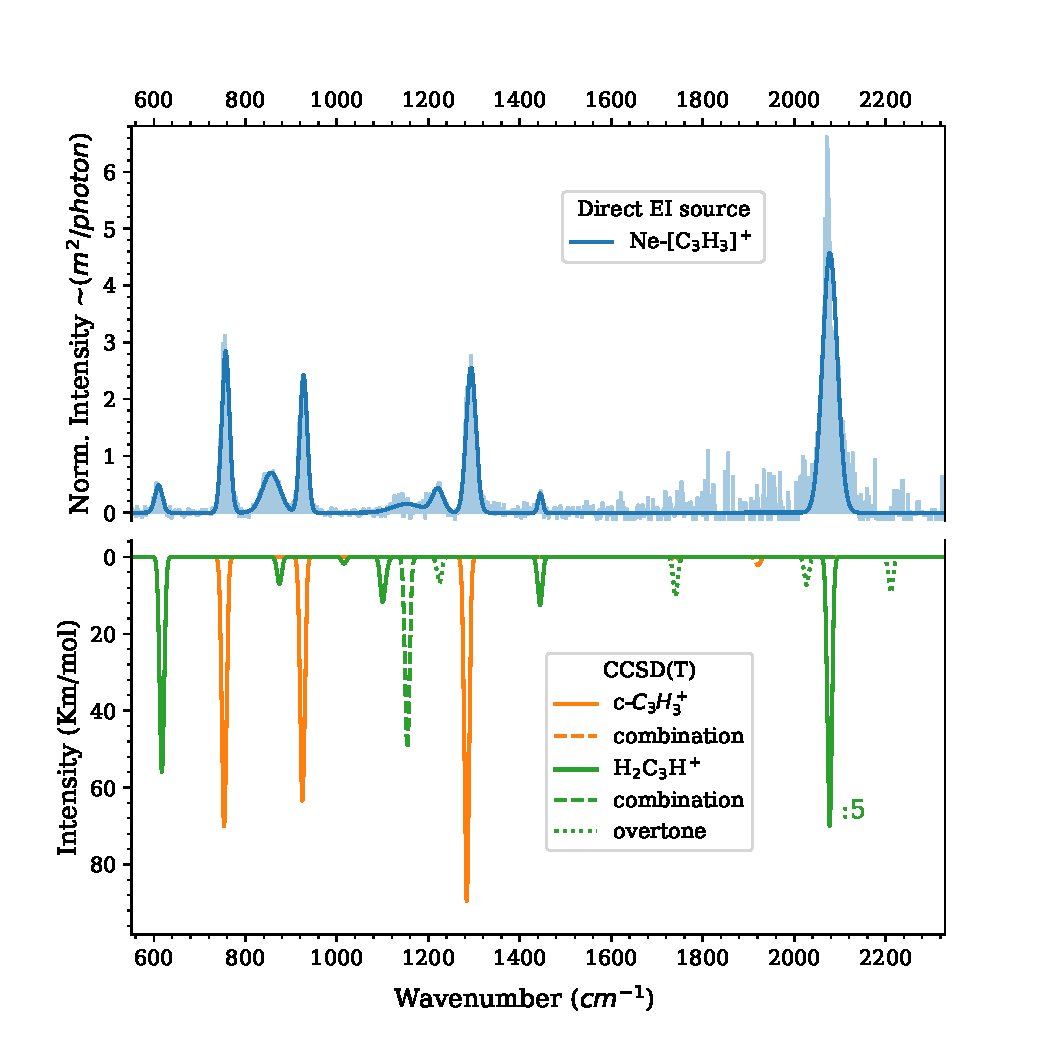
\includegraphics[width=1\textwidth]{chapters/C3H3+ and C3D3+/figures/felix_c3h3+.pdf}
	\caption{The experimental and fitted FELIX IRPD spectrum of Ne-\iso (upper panel) compared to computed frequencies (lower panel) at CCSD(T)/ANO2 combined with the anharmonic correction from CCSD(T)/ANO1 (\linn) and CCSD(T)/ANO0 (\cycn). Only fundamental  (solid line), combination (dashed line) and overtone (dotted line) infrared bands with intensity  $>\, \sim$1~km/mol were included. The theoretical spectrum was folded with a Gaussian corresponding to the FEL linewidth. Peaks marked with \textit{:n} indicate that the depicted peak intensity is scaled down by a factor n, for better visualization.}
	\label{FIG:felix}
\end{figure}

We measured experimental IRPD spectra of \iso isomers under various conditions such as using different ligands (Ne and H$_2$), ion sources (storage and direct EI sources, Figure \ref{FIG:compare_sources} ), and different precursors (propargyl chloride and allene) with ionization energy ranging from (14-70)~eV. The presence of both isomers with varying relative abundance in different conditions was observed and is discussed in detail in Section \ref{iso}. The IRPD vibrational band frequencies obtained from an average spectrum (Figure \ref{FIG:felix}, including data from the propargyl chloride and allene precursors produced in the direct EI source with varying electron impact energies) compared with computed and previous experimental frequencies of both isomers are summarised in Table \ref{tbl1}. The C-H stretching region was measured with the OPO/OPA system only for the allene precursor produced in the storage source, see Figure \ref{FIG:compare_ligands}. The vibrational band assignments based on various computational studies using coupled cluster methods will be discussed for the cyclic and linear isomer in detail in Sections \ref{cyclic} and \ref{linear}, respectively, and for the deuterated species in Section \ref{deut}. The influence of the tagging agent will be discussed in Section \ref{tag}, but was found to be negligible.  \\ 

\clearpage
% \begin{landscape}
\begin{ThreePartTable}
    \small
    \begin{TableNotes}\footnotesize
        \item [a] Frequencies (error in parenthesis). nc indicates not-covered and hyphen $-$ indicates not observed.\\
        \item [b] Measured with OPO/OPA system. The remaining bands are measured with the FELIX free electron laser.\\
        \item [c] Ref. \citep{GLY2012} - Velocity-map imaging photo-electron method.\\
        \item [d] Ref. \citep{Chin2018} -Direct IR absorption spectra of \lin in solid Ar matrix.\\
        \item [t] Tentative assignment.\\
        \item [*] Ref. \citep{RDS2010}.\\
     \end{TableNotes}
    \begin{longtable}{*{16}{c}}

        \caption{Summary of IRPD experimental vibrational band position of Ne-\iso compared to computed fundamental, overtone and combination band frequencies at the CCSD(T)/ANO2 level of theory combined with anharmonic corrections from CCSD(T)/ANO1 (for \lin) and CCSD(T)/ANO0 (for \cyc).}\label{tbl1}\\
        
        \toprule
        Mode & Ne-IRPD\tnote{a} & FWHM & Calc. [Int.]& Ar-IRPD \cite{RDS2010} & VMI-PE\tnote{c} & Ar-Matrix\tnote{d}\\
        & (this work)&\wn&\wn [Km/mol]& \wn& \wn& \wn\\
        
        \midrule
        \endfirsthead
        \\\\\hline \multicolumn{8}{c}{{\bfseries \tablename\ \thetable{} -- continued from previous page}} \\
        \toprule
        Mode & Ne-IRPD\tnote{a} & FWHM & Calc. [Int.]& Ar-IRPD \cite{RDS2010} & VMI-PE\tnote{c} & Ar-Matrix\tnote{d}\\
        & (this work)&\wn&\wn [Km/mol]& \wn& \wn& \wn\\
    
        \toprule
        \endhead
    
        \midrule
        \insertTableNotes
        \\\\\hline \multicolumn{8}{c}{{\bfseries \tablename\ \thetable{} -- continued on next page}} \\ \hline
        \endfoot
        \bottomrule
        % \insertTableNotes
        \endlastfoot
        
    
        \cyc & & & \\\\
        $\nu_{1}(a^{'}_1)$   &    -           & -  & 3179 [0]  & -    \\
        $\nu_{2}(a^{'}_1)$   &    -           & -  & 1610 [0]  & -    \\
        $\nu_{3}(a^{'}_2)$   &    -           & -  & 1024 [0]  & -    \\
        $\nu_{4}(e^{'})$     & 3133(1)\tnote{b}  & 14 & 3127 [189] & 3182 \\
        $\nu_{5}(e^{'})$     & 1293(1)        & 25 & 1284 [88] & 1293 \\
        $\nu_{6}(e^{'})$     & 927(1)         & 19 & 925 [60]  & nc   \\
        $\nu_{7}(a^{''}_2)$  & 757(1)         & 20 & 754 [70]  & nc   \\
        $\nu_{8}(e^{''})$    &    -           & -  & 1000 [0]  & -    \\
        \\
        $\nu_{7}$+$\nu_{8}(e^{'})$ & - & - & 1739 [1]  &      &          &          \\
        $\nu_{3}$+$\nu_{6}(e^{'})$ & - & - & 1921 [2]  &      &          &          \\\\
        \midrule
        
        \lin &&&&& \\\\
        
        %&----------- fundamental ------------\\
        $\nu_{1}(a_1)$                & -           & -  & 3230 [102] & 3238 &          & 3195.3   \\
        $\nu_{2}(a_1)$                & 3003(1)\tnote{b, t} & 9  & 2997 [26]  & 3004 &          & 3000.6   \\
        $\nu_{3}(a_1)$                & 2078(1)     & 32 & 2078 [346] & 2077 & 2086(15) & 2075.2   \\
        $\nu_{4}(a_1)$                & 1445(1)     & 12 & 1444 [12]  & 1445 &          & 1433.2   \\
              
        $\nu_{5}(a_1)$                & 1138(4)     & 31 & 1109 [2]   & 1222 & 1120(15) & 1140     \\
        $\nu_{6}(b_1)$                & 1138(4)     & 31 & 1100 [11]  & 1111 &          & 1105.2   \\
        $\nu_{7}(b_1)$                & 856(1)      & 44 & 875 [7]    & nc   & 858(15)  &          \\
        $\nu_{8}(b_1)$                & nc          & nc & 263 [26]   & nc   &          &          \\
        $\nu_{9}(b_2)$                &3041(1)\tnote{b, t}  & 9  & 3087 [37]  & 3093 &          & 3063.4   \\
        $\nu_{10}(b_2)$               & -           &  - & 1016 [2]   & -    &          &          \\
        $\nu_{11}(b_2)$               & 610(1)      & 12 & 618 [56]   & nc   &          & 606.8    \\
        $\nu_{12}(b_2)$               & nc          & nc & 299 [15]   & nc   &          &          \\\\
     
        %&----------- combination ------------\\
        $\nu_{3}$+$\nu_{5}(a_1)$      & -          &  - & 3168 [7]   &      &          &   \\
        $\nu_{3}$+$\nu_{10}(b_2)$     & -          &  - & 3086 [4]   &      &          &   \\
        $\nu_{4}$+$\nu_{10}(b_2)$     & -          &  - & 2444 [2]   &      &          &   \\
        $\nu_{7}$+$\nu_{8}(a_1)$      & 1138(4)    & 31 & 1154 [50]  &      &          &   \\\\
        
        %&----------- overtone ------------\\
        $2\nu_{4}(a_1)$               &  -          & -  & 2865 [1]   &      &          &   \\
        $2\nu_{5}(a_1)$               &  -          & -  & 2211 [9]   &      & 2247(15) &   \\
        $2\nu_{7}(a_1)$               &  -          & -  & 1741 [10]  &      & 1744(15) &   \\
        $2\nu_{10}(a_1)$              &             & 27 & 2027 [7]   &      &          &   \\
        $2\nu_{11}(a_1)$              & 1222(1)     & 27 & 1224 [7]   &      &          &   \\\\

    \end{longtable}
\end{ThreePartTable}
% \end{landscape}
% \clearpage

\subsection{Cyclic isomer}
\vspace{0.5cm}
\label{cyclic}
The planar \cyc isomer has $D_{3h}$ symmetry with an $A'_1$ vibronic ground state. All of the only four IR active fundamental bands ($\nu_4$, $\nu_5$, $\nu_6$ and $\nu_7$, with the former three being doubly-degenerate) of this energetically lowest-lying aromatic isomer are clearly observed (see Figure \ref{FIG:felix} and \ref{FIG:compare_ligands}, and Table \ref{tbl1}). The band at 3133 \wn\ is assigned to the $\nu_{4}$ asymmetric CH stretching mode, with good agreement to the computed value of 3127~\wn\ and to a previous Ne-IRPD experiment by Roth and Dopfer \cite{Roth2002}, who measured this band at 3130~\wnn. This vibration has also been reported in Ne-matrix at 3130 \wn\ \citep{Wyss2001}. Duncan and coworkers had originally  reported this band around 3182 \wn\ \citep{RDS2010}, but later revised their assignment \citep{Duncan2012}, in line with other experiments \citep{ZDL2014, Roth2002} (see Table \ref{tbl1}), including this work, and previous calculations \citep{BOR2011, HTL2011}. Based on their calculations, Botschwina et al. \citep{BOR2011} argued that the 3182~\wn\ band from Duncan's work could be the $\nu_3$+$\nu_5$ combination band of the linear isomeric form and not the $\nu_{4}$. The fact that we do not observe a band at 3182~\wn\ under conditions preferentially producing the cyclic isomer (see Section \ref{iso}), supports this assignment.
Somewhat puzzling is the appearance of two weak features at 3003 and 3041~\wn\, which are only present in the Ne-tagged spectrum in Figure \ref{FIG:compare_ligands}. No combination or overtone bands of the cyclic isomer are predicted at these frequencies. We tentatively assigned them to the $\nu_2$ and $\nu_9$ modes of the linear isomer. However, the much stronger $\nu_1$ band, observed at 3238~\wn\ in the Ne-IRPD spectrum of \citet{Botschwina2011}, is not detected.\\

The prominent feature $\nu_5(e')$ corresponding to the asymmetric CCC ring stretching is clearly identified at 1293~\wnn. This band was also reported at 1293 \wn\ with Ar-tagging \citep{RDS2010}. Whereas our computed anharmonic frequency at CCSD(T) level is lower by 11 \wnn, the comparison to CCSD(T) quartic force field calculations in combination with variational calculation (VCI 5MR) from \citet{HTL2011} shows good agreement (1296.2 \wnn). The in-plane CH scissoring (927 \wnn, $\nu_6(e')$) and symmetric CH out-of-plane wagging (757 \wnn, $\nu_7(a_2''$)) modes have been measured with an excellent agreement to the computed band positions (see Table \ref{tbl1}), and gas-phase data of these two bands are reported here for the first time. Previously, they were measured by Craig et al. \citep{Craig1986} in various different polycrystalline salts of \cycn $X^{-}$ (with X=SbF$_5$) at  757 \wn\ ($\nu_7$) and 925 \wn\ ($\nu_6$) which agree well with our measurements.\\

\subsection{Linear isomer}
\label{linear}
\vspace{0.5cm}
The linear propargyl isomer with $C_{2v}$ symmetry and an $A_1$ vibronic ground state has 12 fundamental bands, which are all IR active. Previous measurements on the gas-phase \lin isomer include Ar-IRPD spectra (at frequencies above the Ar binding energy ($\sim$ 1000~ \wn)) \citep{RDS2010} and combined vacuum ultraviolet (VUV) laser - velocity-map imaging photoelectron (VMI-PE) spectra obtained only for the $\nu_3$, $\nu_5$ and $\nu_7$ modes \citep{GLY2012}. Here we report and discuss the spectral characterization of the \lin isomer measured in a wide range from 550-3400 \wn. \\

The most prominent $\nu_3(a_1)$ CC triple bond stretching mode at 2078 \wn\ is clearly seen with an excellent agreement to the computed value of the bare ion (2078~\wnn) and the experimental value (2077~\wnn) obtained with Ar-tagging IRPD \citep{RDS2010}. Similarly, the weak band at 1445~\wn\ is assigned to the $\nu_4$ CH$_2$ scissoring vibration. The broad mode identified at 1222~\wn\ can be assigned to $2\nu_{11} (a_1)$ supported by a computed value of the overtone at 1224~\wn\ with substantial intensity larger than other overtone and combination bands in that region. This band was originally assigned to the $\nu_5$ band by Ricks et al. \citep{RDS2010}.  The similarly broad band at 1138 \wn\ with larger uncertainty of 3-4~\wn\ and FWHM of 31~\wn\ is consequently assigned here to a blend of $\nu_5$, $\nu_6$, and $\nu_7+\nu_8$ (intensity of this combination mode might be over-estimated in the calculation, ~50 km/mol, see Figure \ref{FIG:felix}), which our anharmonic CCSD(T) calculations predict at 1109, 1100, and 1154 \wnn, respectively. We should, however, note here that our calculated $\nu_5$ and $\nu_6$ band position are not consistent with the earlier coupled cluster calculations from Botschwina and co-workers \citep{Botschwina2011, BOR2011} and Huang et al. \citep{HTL2011} (see Table \ref{tab:tbl_compare_calc}), who predicted these bands at 1123~\wn\ and 1100~\wnn, respectively, for Ne-tagged \lin and around 1130~\wn\ and 1058~\wn\ (depending on the level of theory), respectively, for the bare ion. The discrepancy for the $\nu_5$ band is likely due to varying theoretical treatment of a Fermi resonance with the $\nu_7+\nu_8$ combination band, which might be further influenced by the (small) perturbation of the Ne-tag. Ricks et al. \citep{RDS2010} observed a doublet feature centered at 1111~\wn\ with Ar as tagging agent, and assigned it to the partly resolved P- and R-branch of the perpendicular $\nu_6$ band.  The $\nu_7$ CCH out-of-plane bending and $\nu_{11}$ CCH in-plane bending bands clearly appear at 856 and 610~cm$^{-1}$, respectively. However, the former band is extremely broad, as is the equivalent band in the fully deuterated species, and was difficult to distinguish from baseline fluctuations in the experiments. We assume a fast predissociation of the Ne-ion complex upon excitation of this mode, leading to life-time broadening. \\

\subsection{Ne-effect}
\vspace{0.5cm}
\begin{figure}
	\centering
	
		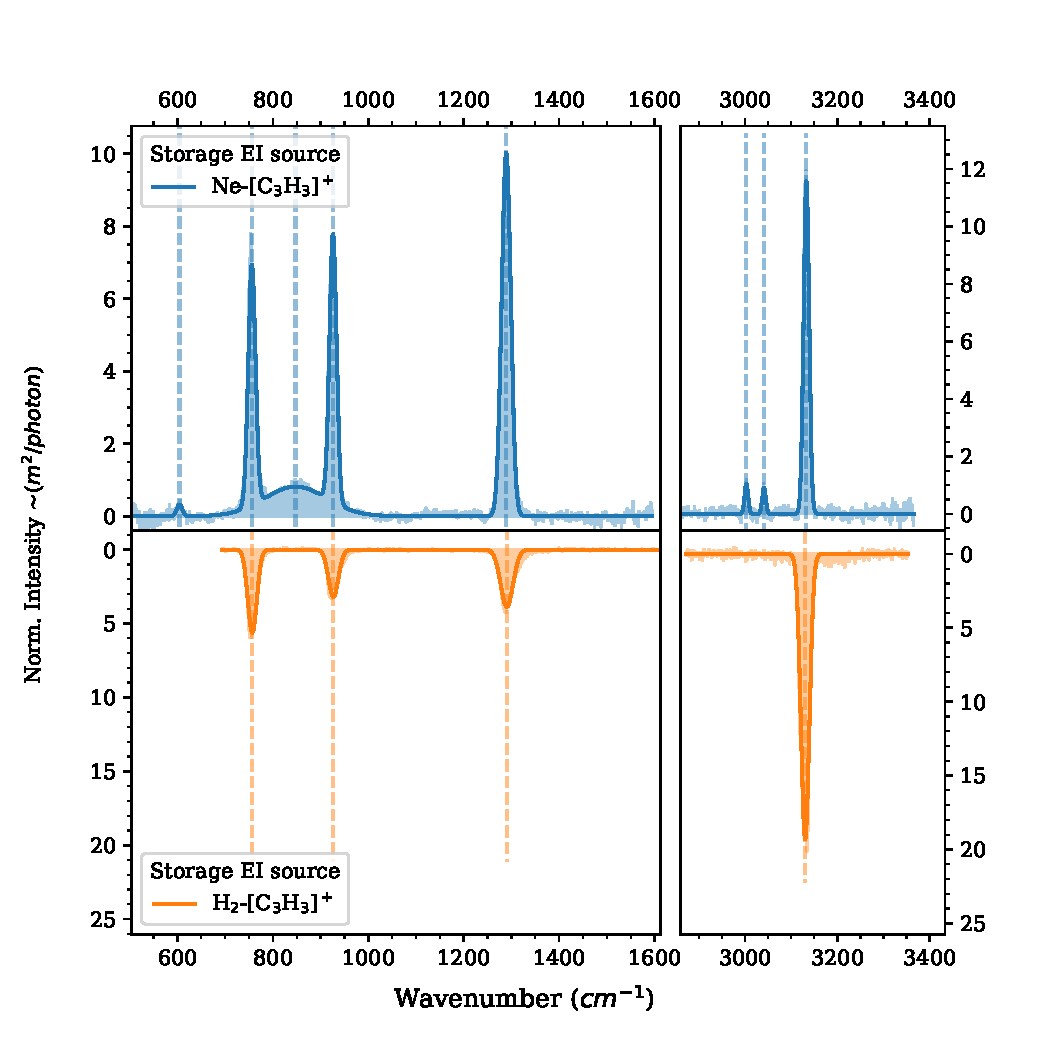
\includegraphics[scale=.7]{chapters/C3H3+ and C3D3+/figures/compare_ligands.pdf}
	\caption{Comparing Ne-\iso (upper panel) and H$_2$-\iso (lower panel) IRPD spectra produced from allene precursor in the storage ion source recorded with FELIX laser and OPO. }
	\label{FIG:compare_ligands}
\end{figure}


\label{tag}
\begin{table}

    \caption{Comparing \lin Ne-IRPD band positions with available computational studies based on coupled cluster methods. All frequencies are in \wn\ units}
    
    \centering
    \begin{tabular}{lccccc}
    
        \hline \hline \\
        Mode& Ne-IRPD & \lin & Ne-\lin & Ar-\lin & \lin   \\
        & (this work)&(this work)$^a$& \multicolumn{2}{c}{\citet{Botschwina2011}$^b$} & \citet{HTL2011}$^c$\\
        \hline\\
        $\nu_{1}(a_1)$  &      & 3230 & 3237(+1) & 3241(+5) & 3239.0 \\
        $\nu_{2}(a_1)$  & 3003$^t$ & 2997 & 2992(+2) & 2996(+6) & 2998.7 \\
        $\nu_{3}(a_1)$  & 2078 & 2078 & 2080(0)  & 2081(+1) & 2082.2 \\
        $\nu_{4}(a_1)$  & 1445 & 1444 & 1446(0)  & 1446(0)  & 1434.4 \\
        $\nu_{5}(a_1)$  & 1138 & 1109 & 1123(0)  & 1119(-4) & 1131.8 \\
        $\nu_{6}(b_1)$  &      & 1100 & 1100(+1) & 1097(-2) & 1058.1 \\
        $\nu_{7}(b_1)$  & 856  & 875  & 873(+1)  & 867(-5)  & 861.9  \\
        $\nu_{8}(b_1)$  &      & 263  & 264(0)   & 281(+17) & 251.7  \\
        $\nu_{9}(b_2)$  & 3041$^t$ & 3087 & 3082(+2) & 3086(+6) & 3071.0 \\
        $\nu_{10}(b_2)$ &      & 1016 & 1017(0)  & 1017(0)  & 1000.6 \\
        $\nu_{11}(b_2)$ & 610  & 618  & 615(0)   & 618(+3)  & 607.7  \\
        $\nu_{12}(b_2)$ &      & 299  & 301(+3)  & 302(+4)  & 294.8  \\
        
        \hline
    \end{tabular}\\
    $^a$ Computed at CCSD(T)/ANO2 combined with anharmonic correction from ANO1\\
    $^b$ $C_s$ min1 structure computed at CCSD(T)-F12/VTZ-F12. Harmonic shift arising from complex formation is given in parentheses.\\
    $^c$ Computed at CCSD(T) QFF with VCI 5MR method. Note that the symmetry labelling of b1 of \citep{HTL2011} is b2 in this paper.\\
    $^t$ Tenative assignment.
    \label{tab:tbl_compare_calc}
\end{table}

We analyzed the effect of Ne complexation on the bare ions' vibrational spectra by comparing them to the computed anharmonic frequencies from various coupled cluster methods of both ligand tagged and untagged species. Botschwina and co-workers \citep{Botschwina2011} had carried out very detailed computational studies on the weak interactions in the ion-ligand complexes of \iso by analyzing the potential energy profile of the complexes while migrating the ligand around the ion-molecule. They have found two $C_s$ and one $C_{2v}$ (highest energy) structures for Ne-\cyc and three $C_s$ minima for Ne-\lin complex ion. They found negligible shifts of order $<3$~\wn\ for the vibrational band positions for both \iso isomers and all ligand-ion isomers. A detailed comparison of ligand-induced band shifts in the spectrum of the \lin isomer is provided in Table \ref{tab:tbl_compare_calc}, where we report only values for the lowest energy $C_s$ structure from \citet{Botschwina2011}. The prominent features $\nu_3$ and $\nu_4$ appear to have no perturbation within 1~\wn\ uncertainty and this is supported by both our Ne-IRPD experiment and calculations on Ne-\linn. The larger discrepancy in the $\nu_7$ band could be reasonably explained by other effects as discussed in section \ref{linear} and \ref{deut}. The four IR active fundamental band of the cyclic isomer of both \iso (except $\nu_5$, see section \ref{cyclic}) and \isoD (section \ref{deut}) also show excellent agreement with the computed fundamental band positions. \\

We can therefore take the IRPD spectra of the Ne-tagged species as an excellent proxy for those of the bare ion, with predicted vibrational shifts much smaller than those for the corresponding Ar-tagged species. Surprisingly, even the use of H$_2$, which has much higher polarizability than Ne (4.5~a.u.  \citep{MH2018} {\textit{vs.}} 2.66~a.u. \citep{SN2018}, respectively) as the tagging agent does not lead to significant shifts, as the comparison in Figure \ref{FIG:compare_ligands} shows, taken under conditions favoring the formation of the \cyc isomer. The predicted small ($\sim 1$~\wnn) splitting of the degenerate e' modes ($\nu_4$, $\nu_5$, and $\nu_6$) of \cyc caused by symmetry-breaking due to the ligand could not be resolved with the given laser linewidth in these experiments. \\



\subsection{Deuterated species}
\label{deut}
\vspace{0.5cm}

Figure \ref{FIG:felix_c3d3+} shows the IRPD spectra of Ne-tagged \isoDn, produced in the direct EI source from fully deuterated allene (C$_3$D$_4$) as a precursor. We covered the range 400-2600~\wnn; using the FEL in its $3^{rd}$ harmonic mode in the range (1800-2600 \wnn), where the substantially shifted C-D stretching bands are expected. The first comprehensive spectral characterization of \cycD was reported by \citet{Craig1986} using poly-crystalline salts. For the linear form \linDn, the C$\equiv$C stretching $\nu_3$ band in Ne-matrix \citep{Wyss2001} and the $\nu_1$-$\nu_6$, $\nu_9$ bands from a recent study of direct absorption of IR bands using isolated solid Ar matrix techniques \citep{Chin2018} were previously reported. However, to the best of our knowledge, there are no reports available on gas-phase data. Hence, here we report the first gas-phase data for \isoD isomers.\\ 

\begin{figure}
	\centering
		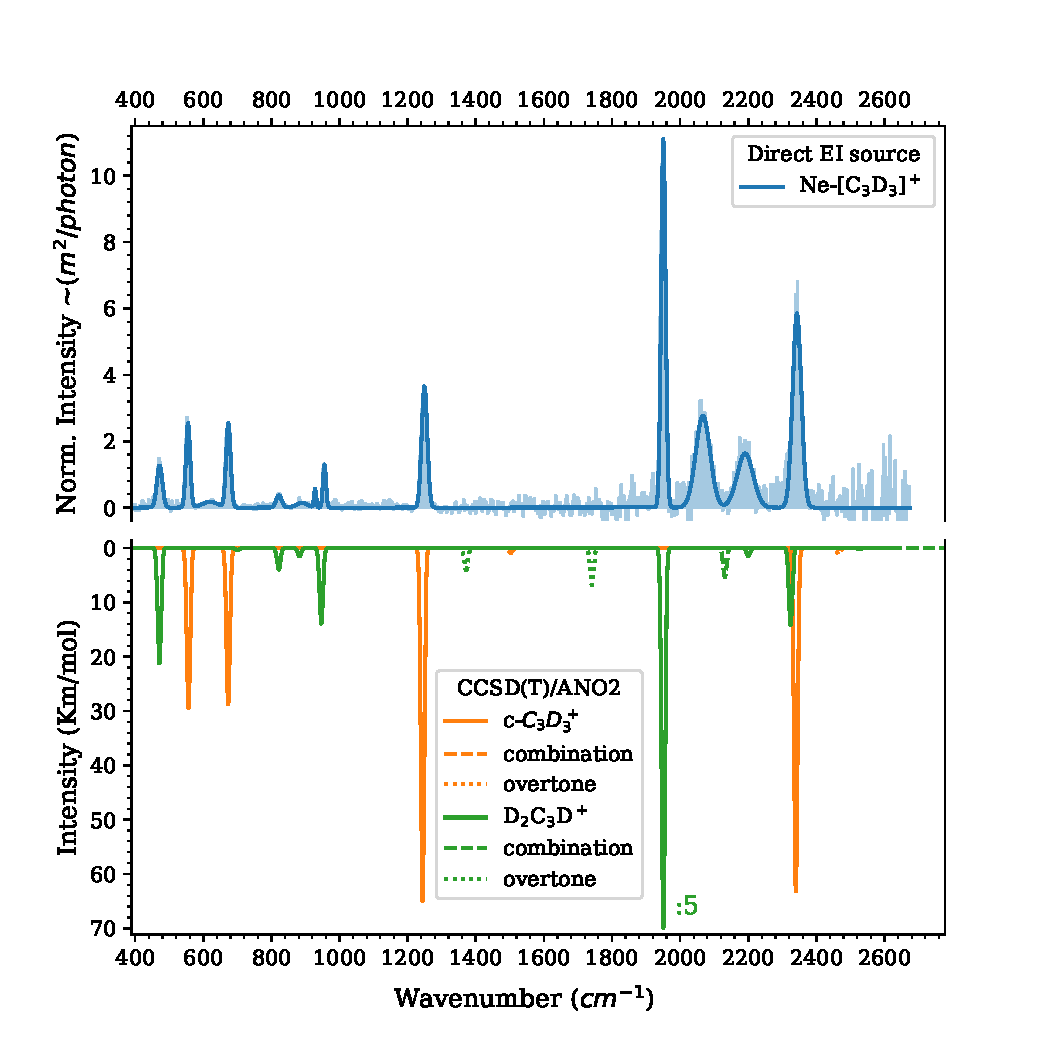
\includegraphics[scale=.7]{chapters/C3H3+ and C3D3+/figures/felix_c3d3+.pdf}
	\caption{The experimental and fitted FELIX IRPD spectrum of Ne-\isoD (upper panel) compared to computed frequencies (lower panel) at CCSD(T)/ANO2 combined with the anharmonic correction from CCSD(T)/ANO1 (\cycDn) and CCSD(T)/ANO0 (\linDn). Only fundamental (solid line) combination (dashed line) and overtone (dotted line) infrared bands with intensity $>\, \sim$1~km/mol were included. The theoretical spectrum was folded with a Gaussian corresponding to the FEL linewidth. Peaks marked with \textit{:n} indicate that the depicted peak intensity is scaled down by a factor n, for better visualization.}
	\label{FIG:felix_c3d3+}
\end{figure}

\clearpage
\begin{landscape}
\begin{ThreePartTable}
    \begin{TableNotes}\footnotesize
        \item [a] Frequencies (error in parenthesis). nc indicates not-covered and hyphen $-$ indicates not observed. $\oplus$ indicates out-of-plane\\
        \item [b] Blended with the $\nu_4$ band of \cycD at 2343~\wn. \\
        \item [c] \citet{Craig1986}, Infrared spectra with polycrystalline salts (\iso BF$_4^-$). \\
        \item [d] \citet{Wyss2001}, Infrared spectra in Neon matrix. \\
        \item [e] \citet{Breslow1970}, Infrared spectra from salts of deuterated cyclopropenyl cation. \\
        \item [f] \citet{Chin2018}, Infrared spectra of \lin in solid Ar matrix\\
     \end{TableNotes}
    \begin{longtable}{*{16}{c}}

        \caption{Summary of IRPD experimental vibrational band position of Ne-\isoD compared to computed fundamental, overtone and combination band frequencies at the CCSD(T)/ANO2 level of theory combined with anharmonic corrections from CCSD(T)/ANO1 (for \cycD) and CCSD(T)/ANO0 (for \linD).}\label{tab:c3d3+}\\
        
        \toprule
        Mode & Assignment & Ne-IRPD         & FWHM & Calc. [Int.] & Prev. Exp.  \\
             &            &(this work) \tnote{a} & \wn  & \wn [Km/mol] & \wn          \\
        
        \midrule
        \endfirsthead
    
        \\\\\hline \multicolumn{8}{c}{{\bfseries \tablename\ \thetable{} -- continued from previous page}} \\
        \toprule
        Mode & Assignment & Ne-IRPD         & FWHM & Calc. [Int.] & Prev. Exp.  \\
             &            &(this work) \tnote{a} & \wn  & \wn [Km/mol] & \wn          \\

        \toprule
        \endhead
    
        \midrule
        \insertTableNotes

        \\\\\hline \multicolumn{8}{c}{{\bfseries \tablename\ \thetable{} -- continued on next page}} \\ \hline
        \endfoot
        \bottomrule
        % \insertTableNotes
        \endlastfoot
    
        \hline
        \hline \\
        
             
        \hline\\
        \cycD &&&& \\\\
        %&----------- fundamental ------------\\
        $\nu_{1}(a^{'}_1)$ & sym. CD str.              &    -    &  -  & 2474 [0]  \\
        $\nu_{2}(a^{'}_1)$ & sym. CCC str.             &    -    &  -  & 1478 [0]  \\
        $\nu_{3}(a^{'}_2)$ & in-plane internal torsion &    -    &  -  & 838  [0]   \\
        $\nu_{4}(e^{'})$   & asym. CD str              & 2343(1) & 30 & 2340 [64] & 2348\tnote{c}, 2344.1(1.0)\tnote{d}, 2327\tnote{e}  \\ 
        $\nu_{5}(e^{'})$   & asym. CCC ring str.       & 1249(1) & 25 & 1244 [65] & 1250\tnote{c}, 1239\tnote{e} \\
        $\nu_{6}(e^{'})$   & in-plane CD scissoring    & 674(1)  & 19 & 673  [28] & 670\tnote{c}, 665\tnote{e} \\
        $\nu_{7}(a^{''}_2)$& sym. CD bending $\oplus$  & 556(1)  & 15 & 556  [27] & 542 \tnote{c}, 542\tnote{e} \\
        $\nu_{8}(e^{''})$  & asym. CD bending $\oplus$ &    -    &  -  & 817  [0]   \\\\
        
        
        %&----------- combination ------------\\
        $\nu_3$+$\nu_5(e^{'})$ &   & 2067(1) & 49 & 2061[0.02]  \\\\
        %$\nu_3$+$\nu_6(e^{'})$ &   &    -     &  -  & 1502[0.9]     \\\\
        
        %&----------- overtone ------------\\
        $2\nu_{5}(e^{'})$  & & - &- & 2466 [1]\\\\
        
        \midrule
        
        \linD &&&&& \\\\
        
        %&----------- fundamental ------------\\
        $\nu_{1}(a_1)$ & CD str.              & -       & -  & 2527 [0.2] & 2487.3\tnote{f} \\
        $\nu_{2}(a_1)$ & CD$_2$ sym str.      & 2193(1) & 55 & 2200 [1.5]  & 2201.0\tnote{f}\\
        $\nu_{3}(a_1)$ & C$\equiv$C str.      & 1951(1) & 32 & 1951[350] & 1955.2(1.0)\tnote{d}, 1942.1\tnote{f}\\
        $\nu_{4}(a_1)$ & CD$_2$ scissoring    & -       & -  & 1201 [0.09] & 1191.7\tnote{f}\\
        $\nu_{5}(a_1)$ & C-C str.             & 956(1)  & 10 & 946 [14] & 938.7\tnote{f}  \\
        %\textcolor{red}{$\nu_8$+$\nu_{10}$ (a$_2$)} &&&& 1056 [0] \\
        $\nu_{6}(b_1)$ & CD$_2$ wag $\oplus$    & 883(3)         & 16 & 882 [1.5] & 891.3\tnote{f}      \\
        $\nu_{7}(b_1)$ & CCD bend $\oplus$      & 619(5)         & 54 & 700 [0.3]                   \\
        $\nu_{8}(b_1)$ & CCC bend $\oplus$      & nc             & nc & 233 [16]                    \\
        $\nu_{9}(b_2)$ & CD$_2$ asym str.       & not resol.\tnote{b} &    & 2324 [14] & 2301.9\tnote{f}     \\
        $\nu_{10}(b_2)$& CD$_2$ wag $\oplus$    & 822(2)         & 20 & 822 [4]                   \\
        $\nu_{11}(b_2)$& CCD bend in-plane      & 472(1)         & 19 & 471 [21]                    \\
        $\nu_{12}(b_2)$& CCC bend in-plane      & nc & nc        &     262 [10] &                   \\\\
        
        %&----------- combination ------------\\
        $\nu_{1}$+$\nu_{7}(b_1)$ & & -   &  -    & 3206 [1]\\
        $\nu_{4}$+$\nu_{5}(a_1)$ & & -   &  -    & 2132 [5]\\
        $\nu_{7}$+$\nu_{8}(a_1)$ & &928(1)& 7.7 & 914 [0.6]\\\\
        %&----------- overtone ------------\\
        $2\nu_{6}(a_1)$ &  & - & -& 1741 [7]\\
        $2\nu_{7}(a_1)$ &  & - & -& 1372 [5]\\\\
    \end{longtable}
\end{ThreePartTable}
\end{landscape}
\clearpage

We clearly identify the four IR active fundamental bands of the cyclic isomer ($\nu_4$, $\nu_5$, $\nu_6$ and $\nu_7$) with excellent agreement to computed fundamental band positions of the untagged species (see Table \ref{tab:c3d3+}). This again demonstrates that the perturbation due to Ne attachment is very small. We also notice an additional feature, with a larger FWHM of 49 \wn, at 2067~\wnn. This band can be assigned to the (weak) predicted combination band $\nu_3$+$\nu_5$ at 2061~\wn.
For the \linD isomer, the $\nu_2$, $\nu_3$, $\nu_5$, $\nu_6$, $\nu_7$, $\nu_{10}$, and $\nu_{11}$ vibrational modes are clearly identified. The most prominent feature is the C$\equiv$C stretching ($\nu_3$) band observed at 1951~\wn. This band was reported at 1955.2~\wn\ in Neon matrix \citep{Wyss2001}. Most bands are in good agreement with theory (see Table \ref{tab:c3d3+}). The $\nu_7$ is assigned to the broad feature centered at 619~\wn\ and shows a large deviation to the calculated band position. Interestingly, a similar situation was observed for the corresponding band in the undeuterated species (see Table \ref{tbl1}). 
%We assign the band at 956~\wn to the $\nu_5$ C-C stretching mode based on the previous Ar-matrix data \citep{Chin2018}, even though we observe a large deviation to the calculated band position of 1052~\wn.
An additional band observed at 928~\wn\ is assigned to the $\nu_7+\nu_8$ combination band predicted at 914~\wnn.\\


\subsection{Isomer quantification}
\label{iso}
\vspace{0.5cm}
\begin{figure}
	\centering
		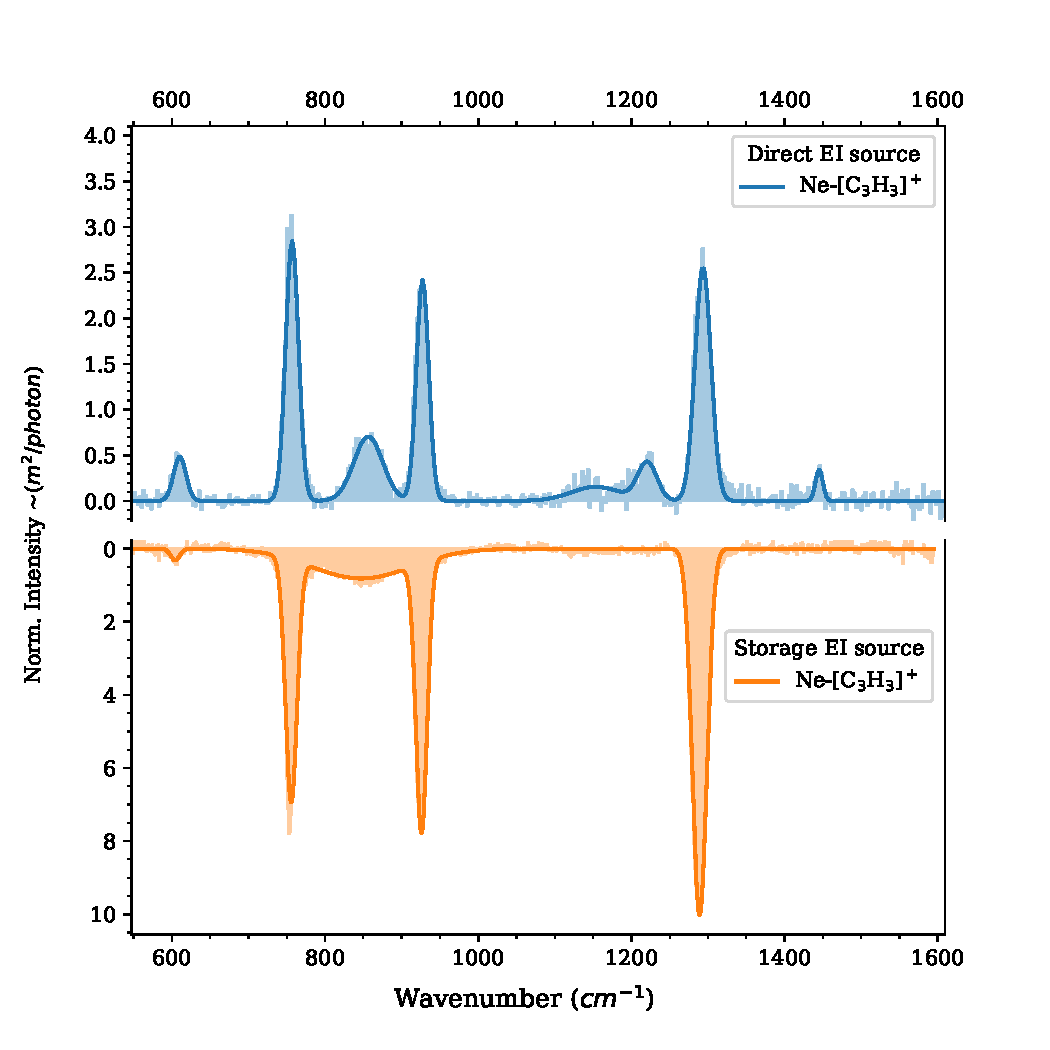
\includegraphics[scale=.7]{chapters/C3H3+ and C3D3+/figures/compare_ion_sources.pdf}
    	\caption{Isomer variation depending on ion production conditions. Upper panel: Experimental IRPD spectrum of Ne-\iso produced from propargyl chloride in the EI source. Lower panel: Same as above but using an allene precursor and the storage ion source.}
    	\label{FIG:compare_sources}
    	
\end{figure}

\begin{figure}
	
	\centering
		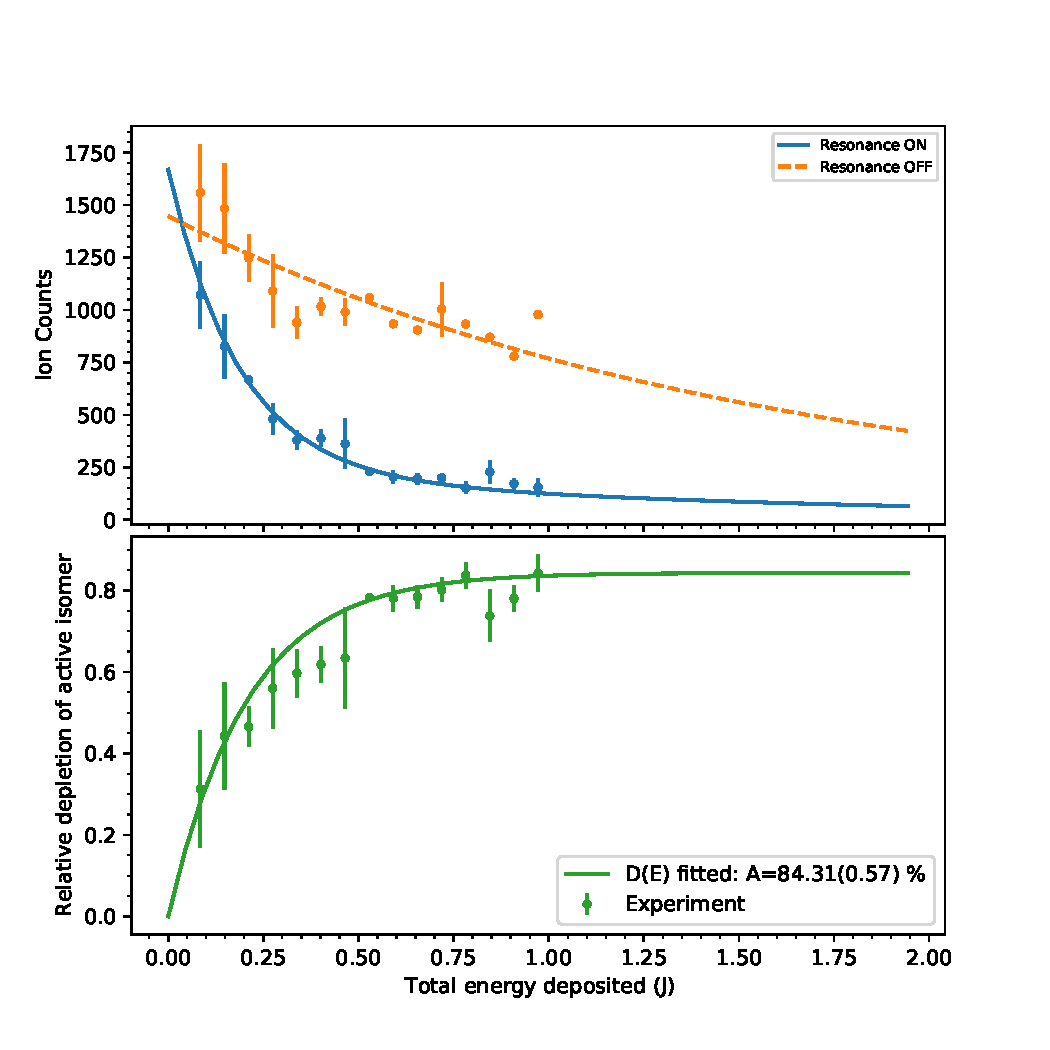
\includegraphics[scale=.7]{chapters/C3H3+ and C3D3+/figures/scan2.pdf}
	\caption{Saturation depletion measurements on the $\nu_5$ band of \cyc, produced from propargyl chloride in the direct EI ion source with ~16.5 eV electrons. Top: On-resonance (blue, at 1293~\wnn, $\nu_5$) and off-resonance (orange, at 1150~\wnn) depletion measurement. Bottom: Relative depletion $D(E)$ as a function of deposited energy $E$, showing saturation at $A=84$\%. }
	\label{FIG:depletion1}
	
\end{figure}

One of the goals of this study was to find ion production methods that preferentially form one of the two \iso isomers, in order to perform subsequent ion-molecule reaction kinetic studies starting with an isomer-pure ionic sample. For this purpose, we used two different neutral precursors, allene and propargyl-chloride, two different ion sources, and a range of electron impact energies.\\

As was described previously \citep{jusko_felion_2019,JSB2018}, it is possible to quantify the percentage of a specific isomer in an isomeric mixture by a saturation depletion method. For this the cluster is resonantly excited at a frequency where only one of the two isomers is active, i.e. absorbs a photon. By increasing the trapping time, thereby increasing the total energy ($E=n\cdot P$) deposited, only the active isomer cluster is depleted until it saturates, and the number of clusters is recorded as a function of deposited energy ($N_{ON}(E)$). To account for additional loss mechanisms from the trap, a second measurement is done with the laser tuned to an off-resonance position, resulting in $N_{OFF}(E)$. From this we can quantify the relative depletion of the particular isomer $D(E)=1-\frac{N_{ON}(E)}{N_{OFF}(E)}$. Assuming an  exponential decay of the clusters with rate coefficients $K_{ON}$ and $K_{OFF}$, respectively, we can write:
\begin{align*}
 N_{OFF}(E) &=  N \cdot e^{-K_{OFF}\cdot E}\\
%\label{eqn:Noff}
 N_{ON}(E) &=  N_a \cdot e^{-(K_{OFF}+K_{ON}) \cdot  E} + N_n \cdot  e^{-K_{OFF} \cdot E}\\
%\label{eqn:Non}
 D(E) &= 1-\frac{N_{ON}}{N_{OFF}} = A \cdot (1-e^{-K_{ON} \cdot E}),\\
\label{eqn:depletion}
\end{align*}
where  $N(=N_a + N_n)$, $N_a$ and $N_n$ are total cluster, active and non-active isomeric cluster counts respectively, and $A=\frac{N_a}{N_a + N_n}$ is the relative abundance of the active isomer. By fitting the experimental data to the corresponding exponentials, we can derive the respective rate coefficients, and, more importantly, the relative abundance of the targeted active isomer, $A$. Such an exemplary fit is shown in Figure \ref{FIG:depletion1}. We should note that this method assumes an equal probability for forming Ne complexes for different isomers. This can be safely assumed, since the binding energies for both Ne-\iso isomers was calculated to be very similar \citep{Botschwina2011}.\\

Although for the \iso ions the cyclic \cyc is substantially lower in energy than the linear \lin form  (28 ~kcal/mol,  \citep{HTL2011}), both isomers were regularly observed in various experiments \citep{RDS2010, Wyss2001, DRM2002}, including this work. Presumably, due to the high isomerization barrier between the two isomers (50~kcal/mol),  both isomers can be formed in the dissociative ionization of the used precursor gases. Theoretical studies have for example shown that the allene and propyne cations, with a linear carbon backbone, can undergo isomerization and ring closure before hydrogen loss, forming dominantly the \cyc isomer upon dissociation \citep{FS1983,MB2008}. 
We indeed observed the cyclic isomer with an abundance of $\sim$81~\% (and the linear form with $\sim$19~\%) upon electron impact ionization of allene in a direct electron impact ionization source, independent of the chosen electron energy in the range $(14-70)$~eV, indicating a constant isomeric branching ratio once the dissociation threshold in the ionization process is reached (allene ionization potential 9.7~eV \citep{YWL1990}, \iso appearance energy 11.4~eV \citep{LOSSING1972}, below 14~eV we could not produce a high enough \iso ion number to perform spectroscopic measurements). When using an ion storage source instead, where the primary ions can undergo subsequent reactions with the neutral gas, we predominantly produced the cyclic form ($\sim$90-95~\%), indicative of the higher reactivity of the linear isomer \linn,  as discussed previously \citep{SLA1982,MMF1994}.\\

In order to increase the formation yield of the propargyl cation \linn, we also used propargyl chloride (ionization energy 10.68(3)~eV, \citep{TWB1975}) as a precursor for direct electron impact ionization. The reasoning here was that the chlorine is expected to be an efficient leaving group after ionization and that thus the propargyl structure is retained in the \iso ionic fragment, as has been proposed in photodissociation studies of the propargyl chloride ion \citep{KR1985}. A comparison between spectra taken under different conditions is given in Figure \ref{FIG:compare_sources}. However, the isomeric ratio shifted only marginally towards the linear isomer, reaching $\sim$22~\% at 60~eV electron impact energy, and being lower ($\sim$16~\%) than for allene ionization at 16.5~eV. \\


To elucidate the formation of the different isomers upon ionization of propargyl chloride, we performed calculations on the potential energy surface of the [ClC$_3$H$_3$]$^+$ system, which are detailed in the Supplementary Information (Figure \ref{fig:C3H3+:fig1}). Our results agree well with earlier calculations at a lower level of theory by \citet{WCK2000}. They indicate that the dissociation to \cyc and Cl via an isomerization to a cyclic form of [ClC$_3$H$_3$]$^+$ is thermodynamically favoured (with a maximum barrier of 53.4~kJ/mol, i.e. 0.55~eV) over the barrier-free dissociation channel to \lin and Cl, which has a relative energy of 81.1~kJ/mol (0.84~eV). Our experimental results indicate that the branching ratio into the two channels stays relatively constant at electron impact ionization energies above 16.5~eV, i.e. 5~eV higher than the \lin appearance energy. This result seems to be contradicting Duncan and co-workers' \citep{RDS2010,Duncan2012} argument that they were predominantly producing the linear isomeric variant using propargyl bromide as a precursor in a discharge coupled to a supersonic expansion. However, for the propargyl bromide cation, the barrier to isomerization to the cyclic variant is slightly higher in energy than the dissociative channel to \lin and Br \citep{KCK1999}, which likely alters the branching ratio in favour of \lin over \cyc. The fact that they were only able to observe a significant signal of the \cyc isomer when running the discharge "hot", i.e. with higher voltages, supports this scenario. In addition, the high inert gas pressure in the nozzle orifice in these experiments might lead to efficient quenching of the isomerization before dissociation. A similar argument might hold for the experiments done by Dopfer and co-workers \citep{DRM2002}, who used electron impact ionization of allene, propyne, 3-chloro-1-propyne, and benzene in a supersonic expansion and identified both \iso isomers with a qualitatively constant ratio of 2:1 (\cyc:\lin) in their spectra. However, earlier reactivity studies pointed towards a higher abundance (approaching 60~\%) of the linear isomer when producing \iso via low energy electron impact ionization of propyne \citep{MMF1994}. We can therefore not exclude that in our experiments the \lin isomer is chemically quenched in the electron impact ion source, where the ions reside for several $\mu$s at neutral gas pressures of $10^{-5}$~mbar. A more effective way to dominantly produce the propargyl cation could be ionization of propargyl iodide \citep{HL1978}.\\

\section{Conclusion}
\vspace{0.5cm}
We investigated broadband gas-phase Ne-IRPD spectra of both linear and cyclic forms of \iso and reported the first gas-phase IR spectra of the corresponding \isoD isomers. Comparison of this new experimental data with theoretical predictions of the vibrational spectra allowed us to benchmark various high-level coupled-cluster methods. All four IR active fundamental bands of cyclic isomer $\nu_4$, $\nu_5$, $\nu_6$ and $\nu_7$ for both \iso and \isoD were reported with very good agreement with computed anharmonic frequencies. The $\nu_6$ and $\nu_7$ gas-phase IR spectra were reported for the first time. We, therefore, can confidently resolve the issues regarding $\nu_4$ assignment for \cyc in \citet{RDS2010}. For the linear isomer, the most prominent vibrational modes $\nu_3$, $\nu_4$, $\nu_7$ and $\nu_{11}$ were clearly identified. The $\nu_5$ and $\nu_6$ modes were identified as a blended broader feature, but not determined with high accuracy. The effect of Neon complexation on the IRPD spectra seems to have only a small influence on the vibrational band positions, once more indicating that the use of weakly bound rare gas ligands such as Ne or He in IRPD action spectroscopy is well suited to obtain IR spectra resembling those of the bare ion. \\

The method of saturation depletion, enabled by the available high FELIX FEL power, was used to investigate the isomeric ratio of \iso produced with different ion source conditions and precursors. Whereas a rather clean production method could be identified for the formation of \cyc, but it has proven difficult to form the more reactive \lin isomer preferentially. Nevertheless, the possibility to quantify the isomer ratio in an isomeric mixture offers great potential for reactivity studies of these ions, which are needed as input for astrochemical models. Furthermore, spectroscopic isomer identification and quantification as described here can be employed to probe the outcome of chemical reactions forming the \iso isomers. Examples are the CH$_3^+ \, + \, $C$_2$H$_{2,4}$ and C$_3$H$^+ \, + \, $H$_2$ reactions proposed to lead to \iso in interstellar clouds and planetary atmospheres \citep{SA1987,Ali2013}.  \\


The accurate spectral characterisation on \iso and \isoD isomers is very important because their fundamental vibrational modes can be used for astronomical searches in the IR region for these ions, e.g. with the upcoming JWST telescope. With a robust experimental methodology and theoretical description now at hand, it would be interesting to extend these studies to the singly and doubly deuterated forms of these species. Whereas the \cyc and \cycD ions belong to the dihedral $D_{3h}$ point group, and do not possess a permanent dipole moment, an effective permanent dipole moment is created upon mono/di D-substitution, because the center of mass is displaced from the center of charge \cite{Huang2011}. This makes these partly deuterated isomers amenable for direct rotational spectroscopy, e.g. using novel action spectroscopic methods that have been developed recently to obtain rotational spectra of reactive ionic species \citep{brunken_laboratory_2014,Brunken2017,Markus2019,thorwirth_pure_2019}. Rotational transition frequencies of these species, as well as for the likewise polar \lin isomer, will enable searches for them in space using sensitive radio telescope, thereby allowing to elucidate their role in interstellar carbon chemistry \citep{SBS2013,LAW2017}.\\

\chapter{Infrared predissociation  spectroscopy of protonated methyl cyanide,  \texorpdfstring{CH$_3$CNH$^+$}{CH3CNH+} }\label{chapter:CH3CNH+}
\chaptermark{Vibrational spectra of \texorpdfstring{CH$_3$CNH$^+$}{CH3CNH+} }

% \begin{center}
%     \includegraphics[width=1\textwidth]{chapters/CH3CNH+/GA3.pdf}
% \end{center}

\blfootnote{This chapter is adapted from : Marimuthu, A. N.; Huis in’t Veld, F.; Thorwirth, S.; Redlich, B.; Brünken, S. Journal of Molecular Spectroscopy, 379, 111477 (2021).}

\newcommand{\pa}{CH$_3$CNH$^+$ }
\newcommand{\pan}{CH$_3$CNH$^+$}

\section*{Abstract}
The gas phase vibrational spectrum of \pa is recorded using a messenger infrared predissociation (IRPD) action spectroscopic method. Vibrational bands were recorded in the $300-1700$~\wn and $2000-3300$~\wn regions making use of the widely tunable free electron laser for infrared experiments, FELIX, coupled to a cryogenic ion trap instrument. Band assignments were aided by high-level quantum-chemical calculations, which showed excellent agreement with the experimental data. Effects of the neon atom used as messenger in the IRPD method are investigated in detail. The data presented here will support astronomical searches for the \pa ion in space, and provides a basis for high-resolution ro-vibrational and pure rotational studies in vibrationally excited states.
\clearpage


\section{Introduction}

Methyl cyanide (CH$_3$CN, also known as acetonitrile) was among the first polyatomic molecules detected during radio-astronomical observations of the interstellar medium (ISM) \cite{SJP1971}. It has since been detected in a variety of galactic sources, covering most evolutionary stages from dense cold cores \cite{GMO2016,VLW2019}, via low- and high-mass star-forming regions \cite{AGM2018,FOG2015} and protoplanetary disks \cite{OGF2015} to photodissociation regions \cite{GPG2014} and circumstellar envelopes \cite{ACQ2015}. CH$_3$CN has also been detected in the atmosphere of Saturn's moon Titan \cite{MHB2002,Thelen2019AbundanceObservations,IST2020}.

As methyl cyanide has a proton affinity of $788(8)$~kJ/mol \cite{KFM1986}, much larger than that of H$_2$, its protonated version (\pan) might form effectively via exothermic proton transfer from H$_3^+$ to CH$_3$CN in the interstellar medium \cite{ILB1981}. Another effective formation pathway of protonated methyl cyanide is via radiative association of CH$_3^+$ and HCN. The latter pathway, followed by dissociative recombination, was suggested to be the major gas-phase route for the interstellar synthesis of methyl cyanide (and its isocyanide isomer) \cite{HM1979,DMH1985, VKH2008}. Despite its dominant role in the formation of the ubiquituous methyl cyanide molecule, previous searches for \pa in the interstellar medium were unsuccessful \cite{TAF1990}. Protonated methyl cyanide, as well as other protonated nitriles, have, however, been detected in Titan's upper atmosphere by the Ion Neutral Mass Spectrometer (INMS) on board the Cassini spacecraft \cite{VYA2006}. It is dominantly formed by protonation of CH$_3$CN via reactions with the highly abundant ions HCNH$^+$ and C$_2$H$_5^+$, whose deprotonated variants have a lower proton affinity than methyl cyanide \cite{VYM2007}.

The pure rotational spectrum of protonated methyl cyanide has been studied extensively in the microwave \cite{GAM2000} and submillimeter-wave region \cite{AHH2006}.
Several infrared studies on \pa exist, including matrix-isolation FT-IR \cite{Frankowski2005} of its CH and NH stretching bands, infrared-predissociation (IRPD) action spectroscopy of its complex with H$_2$ in the H$_2$ and NH stretching region \cite{DRO1999}, and high-resolution gas-phase absorption spectroscopy on the $\nu_1$ NH stretching fundamental band of the bare ion \cite{Amano1988, Amano1992}. All these studies focus on the stretching bands located at wavelengths below 3.4~$\mu$m, or at wavenumbers above 2900~\wn, respectively, and to date no spectroscopic data on its low-lying vibrational modes existed.

In this study we recorded the vibrational spectrum of gas-phase \pa over a broad frequency range  ($300-1700$ and $2000-3300$~\wnn) covering all fundamental modes except the previously studied NH stretching band. Experiments were performed using Ne-tagging infrared-predissociation spectroscopy in a cryogenic ion trap coupled to the powerful and widely tunable FELIX (Free Electron Lasers for Infrared eXperiments, \cite{oepts_free-electron-laser_1995}) free-electron IR lasers. These data can serve as reference data for future laboratory infrared studies at high spectral resolution as well as astronomical searches for this important ion in space, e.g., with the upcoming James Webb Space Telescope (JWST). 


\section{Methods}

\subsection{Experimental details}

\begin{figure}
	\centering
		\includegraphics[scale=.6]{chapters/CH3CNH+/figures/masspec_log.pdf}
	\caption{Upper panel: Mass spectra of ions produced from electron impact ionization ($\sim$30eV) in a storage ion source. See text for discussion of the main peaks Lower panel: { Mass filtered \pa (m/z = 42, $<10$~\% contribution at m/z = 41 and 43) together with tagged \pan -Ne (m/z = 62, also \pan -$^{22}$Ne at  m/z = 64) species produced in the cryogenic ion trap. Additional weaker contributions at m/z = 60, 70, and 74 stem from tagging with residual H$_2$O, N$_2$, and O$_2$, respectively.}  }
	\label{FIG:CH3CNH+:masspec}
\end{figure}

The vibrational spectrum of \pa was recorded using the FELion cryogenic 22-pole ion trap instrument.  A detailed account of the FELion instrument is provided in Section \ref{sec:felion} and the infrared-predissociation (IRPD) of in-situ rare gas tagged cold molecular ions in Section \ref{subsec:action:methods:vibrational:IRPD}. Here we only give a brief account of details specific to the \pa ion.

Protonated methyl cyanide (m/z = 42) was produced by electron impact ionization (EI, electron energy 30~eV) from neutral methyl cyanide (Sigma Aldrich, $>99.9$\%) in a Gerlich-type storage ion source (SIS) \cite{Gerlich1992}, where primary ions produced by EI are accumulated for the duration of an experimental cycle (of the order of seconds). { The precursor gas was admitted either pure or diluted with He at a ratio of 1:3 to the ion source chamber at a pressure of $\sim 10^{-5}$~mbar. Self-protonation of the primarily formed methyl cyanide radical cations with neutral methyl cyanide \cite{TFI2010}, led to effective production of \pa (see Figure \ref{FIG:CH3CNH+:masspec}). Additional prominent mass-peaks in the mass-spectrum are due to the radical methyl cyanide cation (m/z = 41) and the hydrogen loss fragment CH$_2$CN$^+$ with m/z = 40. Interestingly, we observe the appearance of a mass-peak at m/z = 54, which is likely caused by a reaction of CH$_2$CN$^+$ with neutral methyl cyanide in the storage source \cite{ATF2012}. Fragment ions, including their protonated  forms are apparent in the range m/z = $26 - 32$, contamination from water and air leads to additional contributions at m/z = 18 (not shown), 28, and 32.} 

For spectroscopic IRPD experiments a few 10~ms long pulse of ions is extracted from the respective source and filtered for the mass of interest, m/z = 42 in the case of \pa by a quadrupole mass filter before entering the 22-pole ion trap which is held at a fixed temperature in the range 6.1-7~K for experiments using Ne as tagging gas. Around 10-20~ms before the ions enter the trap, an intense 80-150~ms long Ne:He pulse (1:3 mixing ratio and number density of $\sim 10^{15}$~cm$^{-3}$) is admitted to the trap, leading to efficient collisional cooling of the ions to the ambient temperature. Under these conditions, { around 20~\% of the \pa ions form weakly bound complexes with Ne, see Figure \ref{FIG:CH3CNH+:masspec}.} The ions are stored for several seconds in the ion trap and are exposed to several laser pulses before extraction. An IR-PD spectrum is recorded by mass-selecting and counting the \pan-Ne complex ions while tuning the laser frequency $\nu$. A relative depletion $D=1-\frac{N_{ON}(\nu)}{N_{OFF}}$ in the number of complex ions $N_{ON}(\nu)$ from the baseline value $N_{OFF}$ is observed upon resonant vibrational excitation. To account for varying laser pulse energy $P$, pulse number $n$, and for saturation effects, the signal is normalized prior to averaging using $I=\frac{- ln(N_{ON}(\nu)/N_{OFF})}{n\cdot P/(h\nu)}$, giving the intensity $I$ in units of relative cross-section per photon. 
After normalizing each measurement in this way, the final spectrum is then obtained by averaging using statistical binning with a typical bin size of 2.5~\wn. Line parameters such as band positions, intensities, and line widths (fwhm) are then obtained by fitting a multi-component Gaussian function to the experimental data, also providing statistical errors of the line parameters.


The vibrational IRPD spectra were recorded using the IR radiation of FEL-2 of the FELIX Laboratory in the frequency region 300-1700 \wn, and in the range 2000-3300 \wnn employing the $3^{rd}$ harmonic mode of the FEL. The laser was operated at 10~Hz with macro pulse energies in the interaction region between 1.5-60~mJ, and for each datapoint $n=$3-66 pulses were admitted depending on the signal strength. The FEL was optimized for narrow bandwidth with a full width at half-maximum (fwhm) of $0.3-1$~\% of the center wavelength.\\

\subsection{Computational details} 

\begin{figure}
	\centering
		\includegraphics[scale=.3]{chapters/CH3CNH+/figures/molecule.pdf}
		\caption{Computed equilibrium geometry (C$_{3v}$ symmetry) for \pa based on (fc-CCSD(T)/ANO2, \textbf{\textit{ae-CCSD(T)/cc-pwCV5Z}}) level of theory. Bond lengths and angles are in $\mathring{A}$ and deg$^{\circ}$ respectively.}
	\label{FIG:molecule}
\end{figure}

The stability and relative energies of the [C$_2$H$_4$N]$^+$ isomeric family have been extensively studied previously at various levels of theory, showing N-protonated acetonitrile (\pa, $^1A_1$, C$_{3v}$ symmetry) to be the global minimum structure \cite{wuerthwein_1984, Cerqueira2020}.
In the present study we have investigated \pa at the coupled-cluster singles and doubles (CCSD) level augmented by a perturbative treatment of triple excitations, CCSD(T)  \cite{raghavachari_chemphyslett_157_479_1989}, in combination with atomic natural orbital (ANO0, ANO1, and ANO2) basis sets from Alml\"of and Taylor \cite{almlof_JCP_86_4070_1987} as well as the
correlation-consistent valence basis set cc-pVDZ \cite{dunning_gaussian_1989}
in the frozen core (fc) approximation. A best estimate equilibrium structure has been calculated using the cc-pwCV5Z basis set \cite{peterson_JCP_117_10548_2002} using all electrons in the correlation treatment.
Equilibrium geometries of \pa have been calculated using analytic gradient techniques  \cite{watts_chemphyslett_200_1-2_1_1992} and our results for the bare ion (Figure \ref{FIG:molecule}) match well with an earlier report by Botschwina \cite{Botschwina2000} who employed ab initio methods up to the CCSD(T)/cc-pCVQZ level. Harmonic frequencies were subsequently computed by numerical differentiation of
gradients \cite{lee_analytic_1991,watts_coupledcluster_1993}.
For anharmonic calculations, second-order vibrational perturbation theory (VPT2) \cite{mills_alphas} has been employed. All calculations have been carried out using the CFOUR program package  \cite{cfour_JCP_2020,harding_parallel_2008}. The CCSD(T) method in combination with ANO basis sets has been shown previously to provide vibrational wavenumbers of high quality  \cite{mccaslin_MolPhys_111_1492_2013,thorwirth_JMS_251_220_2008}, and we have recently applied it successfully for a vibrational study of [C$_3$H$_3]^+$ isomers and isotopologues \cite{Marimuthu2020LaboratorySpectroscopy}.

Additionally, we have performed potential energy scans to find the lowest energy structure of \pa complexed with Ne, as outlined in Section \ref{Neon influence}. These studies were conducted at the CCSD(T)/cc-pVDZ and CCSD(T)/ANO0 level of theory using the PSI4 program package \cite{PBL2017}. The potential energy surface as a function of H-Ne distance of the lowest energy conformer was then further investigated to account for Basis Set Superposition Errors \cite{liu_accurate_1973} using i) the counter-poise (CP) method introduced by Boys and Bernardi \cite{boys_calculation_1970}, i.e. by calculating CP-corrected CCSD(T) interaction energies at each geometry, and ii) higher-order symmetry-adapted perturbation theory, SAPT2+3/cc-pVDZ  \cite{jeziorski_perturbation_1994, hohenstein_density_2010}. In all PES calculations the geometry of the bare ion was kept fixed to its equilibrium structure calculated at the same level of theory. No zero-point vibrational energy (ZPE) corrections were applied to the derived binding energies.

\section{Results and discussions}
\subsection{Vibrational spectroscopy of \texorpdfstring{\pa}{}}

\begin{figure}
	\centering
		\includegraphics[scale=.7]{chapters/CH3CNH+/figures/felix_1_rev.pdf}
	\caption{The experimental and fitted FELIX IRPD spectrum of \pan-Ne (upper panel) compared to the computed anharmonic (VPT2) frequency values (lower panel) of \pa at the fc-CCSD(T)/ANO2 level of theory showing fundamental (orange, solid line), combination and overtone (orange, dashed line) bands. NOTE: /n and *n indicates that the computed intensities are divided or multiplied, respectively, by a  factor n for better visualisation }
	\label{FIG:felix_1}
	
\end{figure}

\begin{figure}
	\centering

		\includegraphics[scale=.7]{chapters/CH3CNH+/figures/felix_2_rev.pdf}
	\caption{The experimental and fitted FELIX IRPD spectrum of \pan-Ne (upper panel) but using FELIX in 3$^{rd}$ harmonic mode, compared to the computed anharmonic (VPT2) frequency values (lower panel) of \pa at the (fc)-CCSD(T)/ANO2 level of theory.}
	\label{FIG:felix_2}
	
\end{figure}

The measured IRPD spectra for [C$_2$H$_4$N]$^+$  with Ne as a tagging agent are displayed in Figures \ref{FIG:felix_1} and \ref{FIG:felix_2}, compared to the calculated spectrum of the energetically lowest lying isomer, \pan. Based on these results we can infer that only the most stable isomer \pa, i.e. N-protonated methyl cyanide, is produced via self-protonation in our storage ion-source. By exposing the complexes to $>100$ FEL shots on resonance with the strong band at 898~\wnn we could verify that $>95$\% of the complexes dissociate, i.e. that only one isomeric variant absorbing at this specific frequency is present in the ion trap. The \pa structure with C$_{3v}$ symmetry has 10 IR active fundamental modes of E and A$_1$ symmetry. As can be clearly seen in Figure \ref{FIG:felix_1} and \ref{FIG:felix_2}, we have covered and assigned all fundamental modes, except the high-lying NH-stretching mode that was out of the range of the FEL. Four remaining weak to moderately strong features could be assigned to combination and overtone modes predicted by the anharmonic force field calculations. The fitted band positions and assignments are summarized in Table \ref{tbl1:CH3CNH+}.
Several remaining, weak features, e.g., between $600-700$~\wnn are likely due to combination bands of the bare ions fundamental modes and those involving the weakly bound Ne atom. The observed transitions for \pan-Ne are in very good agreement with the computed values of the  bare ion \pa (see Table \ref{tbl1:CH3CNH+}). For most bands the deviation is less than 10~\wn, except for the CNH bending mode, and the overtone and combination modes, as will be discussed below. The influence of the neon-tag on the vibrational band positions is discussed in more detail in section \ref{Neon influence}.

The lowest energy CCN bending mode $\nu_{10}$ is clearly observed at 385~\wn\\ with excellent agreement to the anharmonic predicted value at 384~\wn. The most prominent feature, the $\nu_9$ CNH bending mode, is observed at 596~\wn, almost 20~\wnn blue-shifted from the predicted band position of the bare ion. This shift is likely caused by the attached neon atom, that binds to the proton involved in this bending mode (see section \ref{Neon influence}). The combination band of these two bending modes (CCN and CNH) was also observed at 982~\wnn as a weak feature. Also a very clear feature of the CNH first overtone appears at 1179~\wn. In general the computed values for the combination and overtone modes are $10-20$~\wnn shifted with respect to the experimentally observed bands. The CC stretching frequency $\nu_5$ is measured at 898~\wnn with a $\sim7$~\wnn blue-shift from the predicted value 890~\wn. The weak combination mode of the CC stretching with the CNH bending mode also appears with sizable intensity at 1445~\wn. We could also clearly observe the CH$_3$ vibrations, i.e. the $\nu_8$ wagging and $\nu_7$ scissoring, at 1026 and 1421~\wnn respectively (see vibrational displacement vectors given in the Supplementary Information Figure \ref{fig:CH3CNH+:fig2}). The former also forms a combination mode with the CCN bending at 1405~\wnn which matches well with the predicted value at 1397~\wnn (intensity over $14$~km/mol). The $\nu_4$ CH$_3$ umbrella like bending mode appears at 1364~\wnn very close to the predicted value at 1361~\wn. The $\nu_3$ CN stretching,  CH$_3$ $\nu_2$ symmetric and $\nu_6$ asymmetric stretching bands were measured with FELIX 3$^{rd}$ harmonic mode (see Figure \ref{FIG:felix_2}) resulting in lower resolution and signal-to-noise spectra, reflected in the larger experimental error of these lines. In addition, measurements of the two CH stretching bands suffered from calibration issues of the grating spectrometer used to determine the FEL frequency, reflected in their large systematic errors of 10~\wn.

\clearpage
\begin{landscape}
\begin{ThreePartTable}
    \begin{TableNotes}\footnotesize
        \item [a] \pa \& \pan-Ne (C$_{3v}$ symmetry isomer) harmonic frequencies were computed at the  CCSD(T)/ANO0 level of theory and their differences were added as Neon contribution to \pa frequencies computed at CCSD(T)/ANO2 (see section \ref{Neon influence}).\\
        \item [b] Frequencies (error in parentheses). nc indicates not covered.\\
        \item [c] Ne-matrix, Ref \cite{Frankowski2005}\\
        \item [d] Gas-phase, Ref \cite{Amano1992}\\
     \end{TableNotes}
    \begin{longtable}{*{16}{c}}

    \caption{Summary of IRPD experimental vibrational band position of \pan-Ne and comparison to computed values. Vibrational frequencies are in \wn [calc. intensities in km/mol]}\label{tbl1:CH3CNH+}\\

        \toprule
        \multicolumn{3}{c}{Vibrational symmetry and mode} & \multicolumn{2}{c}{CCSD(T)/ANO2} & Ne-IRPD\tnote{b} & prev. work   \\
            \multicolumn{3}{c}{(\pa, C$_{3v}$, $^1$A$_1$ ground state)} & (VPT2, anh.) & Ne corrected\tnote{a} &(this work) & \\\\
            \hline\\
            \multicolumn{3}{l}{Fundamental bands}&&\\\cline{1-3}\\
        
        \midrule
        \endfirsthead
        \\\\\hline \multicolumn{8}{c}{{\bfseries \tablename\ \thetable{} -- continued from previous page}} \\
        \toprule
        \multicolumn{3}{c}{Vibrational symmetry and mode} & \multicolumn{2}{c}{CCSD(T)/ANO2} & Ne-IRPD\tnote{b} & prev. work   \\
            \multicolumn{3}{c}{(\pa, C$_{3v}$, $^1$A$_1$ ground state)} & (VPT2, anh.) & Ne corrected\tnote{a} &(this work) & \\\\
            \hline\\
            \multicolumn{3}{l}{Fundamental bands}&&\\\cline{1-3}\\
    
        \toprule
        \endhead
    
        \midrule
        \insertTableNotes
        \\\\\hline \multicolumn{8}{c}{{\bfseries \tablename\ \thetable{} -- continued on next page}} \\ \hline
        \endfoot
        \bottomrule
        % \insertTableNotes
        \endlastfoot
            
            
            $\nu_{10}$ & E     & CCN bend            & 384  [4.5]    & 386  & 385  (1)  & \\
            $\nu_{9}$ & E      & CNH bend            & 577  [132.3]  & 595  & 596  (1)  & \\
            $\nu_5$ & A$_1$    & CC str.             & 890  [4.2]    & 891  & 898  (1)  & \\
            $\nu_8$ & E        & CH$_3$ wagging      & 1024 [6.4]    & 1025 & 1026 (1)  & \\
            $\nu_4$ & A$_1$    & CH$_3$ umbrella     & 1361 [13.8]   & 1362 & 1364 (1)  & \\
            $\nu_7$ & E        & CH$_3$ scissoring   & 1429 [1.5]    & 1429 & 1421 (1)  & \\
            $\nu_3$ & A$_1$    & CN str.             & 2305 [46.9]   & 2305 & 2307 (2)  & \\
            $\nu_2$ & A$_1$    & CH3 sym. str.       & 2930 [48.3]   & 2930 & 2924 (10) & \\
            $\nu_6$ & E        & CH3 asym. str.      & 3002 [22.7]   & 3002 & 2996 (10) & 2946.5 [53]\tnote{c} \\
            $\nu_1$ & A$_1$    & NH str.             & 3525 [654.7]  & 3516 & nc        & 3500.6 [677]\tnote{c}, 3527.29\tnote{d} \\
            \\
            \multicolumn{3}{l}{Overtones and Combination bands}&&\\\cline{1-3}\\\\
            $\nu_{10}+\nu_9$  & A$_1$& CCN bend + CNH bend     & 962 [0.01]  & & 982 (2) \\
            $2\nu_{9}$       & A$_1$& CNH bend (2)            & 1157 [16.3] & & 1179 (1)\\
            $\nu_{10}+\nu_8$  & A$_1$&  CCN bend + CH$_3$ wag  & 1397 [14.4] & & 1405 (1)\\
            $\nu_9+\nu_5$ & E & CC str. + CNH bend             & 1467 [0.03] & & 1445 (1)\\

    
    \end{longtable}
\end{ThreePartTable}
\end{landscape}
\clearpage
% \newgeometry{left=2cm}
% \begin{table}

%     \caption{Summary of IRPD experimental vibrational band position of \pan-Ne and comparison to computed values. Vibrational frequencies are in \wn [calc. intensities in km/mol]}\label{tbl1:CH3CNH+}
%         \centering
%         \small
%         \begin{tabular}{cccllrc}
    
%             \\\hline \hline\\
            
%             \multicolumn{3}{c}{Vibrational symmetry and mode} & \multicolumn{2}{c}{CCSD(T)/ANO2} & Ne-IRPD\textsuperscript{b} & prev. work   \\
%             \multicolumn{3}{c}{(\pa, C$_{3v}$, $^1$A$_1$ ground state)} & (VPT2, anh.) & Ne corrected$^a$ &(this work) & \\\\
%             \hline\\
%             \multicolumn{3}{l}{Fundamental bands}&&\\\cline{1-3}\\
            
%             $\nu_{10}$ & E     & CCN bend            & 384  [4.5]    & 386  & 385  (1)  & \\
%             $\nu_{9}$ & E      & CNH bend            & 577  [132.3]  & 595  & 596  (1)  & \\
%             $\nu_5$ & A$_1$    & CC str.             & 890  [4.2]    & 891  & 898  (1)  & \\
%             $\nu_8$ & E        & CH$_3$ wagging      & 1024 [6.4]    & 1025 & 1026 (1)  & \\
%             $\nu_4$ & A$_1$    & CH$_3$ umbrella     & 1361 [13.8]   & 1362 & 1364 (1)  & \\
%             $\nu_7$ & E        & CH$_3$ scissoring   & 1429 [1.5]    & 1429 & 1421 (1)  & \\
%             $\nu_3$ & A$_1$    & CN str.             & 2305 [46.9]   & 2305 & 2307 (2)  & \\
%             $\nu_2$ & A$_1$    & CH3 sym. str.       & 2930 [48.3]   & 2930 & 2924 (10) & \\
%             $\nu_6$ & E        & CH3 asym. str.      & 3002 [22.7]   & 3002 & 2996 (10) & 2946.5 [53]$^c$ \\
%             $\nu_1$ & A$_1$    & NH str.             & 3525 [654.7]  & 3516 & nc        & 3500.6 [677]$^c$, 3527.29$^d$ \\
%             \\
%             \multicolumn{3}{l}{Overtones and Combination bands}&&\\\cline{1-3}\\\\
%             $\nu_{10}+\nu_9$  & A$_1$& CCN bend + CNH bend     & 962 [0.01]  & & 982 (2) \\
%             $2\nu_{9}$       & A$_1$& CNH bend (2)            & 1157 [16.3] & & 1179 (1)\\
%             $\nu_{10}+\nu_8$  & A$_1$&  CCN bend + CH$_3$ wag  & 1397 [14.4] & & 1405 (1)\\
%             $\nu_9+\nu_5$ & E & CC str. + CNH bend             & 1467 [0.03] & & 1445 (1)\\
%             \\\hline\hline\\
%         \end{tabular}\\
    
%     $^a$ \pa \& \pan-Ne (C$_{3v}$ symmetry isomer) harmonic frequencies were computed at the  CCSD(T)/ANO0 level of theory and their differences were added as Neon contribution to \pa frequencies computed at CCSD(T)/ANO2 (see section \ref{Neon influence}).\\
%     $^b$ Frequencies (error in parentheses). nc indicates not covered.\\
%     $^c$ Ne-matrix, Ref \cite{Frankowski2005}\\
%     $^d$ Gas-phase, Ref \cite{Amano1992}\\
    
% \end{table}
% \restoregeometry
% \normalsize

\subsection{Prediction of rotational spectroscopic parameters}

The above discussion clearly shows that anharmonic calculations at the \\CCSD(T)/ANO2 level provide a reliable means to predict vibrational band positions for \pan. In addition we present in Table \ref{tbl2} the calculated equilibrium and ground state rotational constants and compare the latter to experimentally derived values \cite{GAM2000,AHH2006} and a previous calculations using the aug-cc-pVQZ basis set \cite{Cerqueira2020}. 
From the relative deviations of the calculated spectroscopic constants to the experimental values, it is obvious that the fc-CCSD(T)/ANO2 calculation of $B_0$ (from the equilibrium rotational constant B$_e$ complemented by the zero point vibrational contribution $\Delta B_0$, see below) are slightly further off than the CCSD(T)/aug-cc-pVQZ values
reported earlier \cite{Cerqueira2020}, whereas centrifugal distortion constants show a similar accuracy. 
Best estimate ground state rotational constants have been calculated here using a hybrid approach with the equilibrium structure
calculated at the ae-CCSD(T)/cc-pwCV5Z and the zero-point vibrational corrections $\Delta B_{0}=\frac{1}{2}\sum{\alpha_i^B}$ (analogous for $A$) from rotation-vibration interaction constants $\alpha_i$ calculated at the fc-CCSD(T)/ANO2 level of theory (see Table \ref{tab:CH3CNH+:tab4} in the Supplementary Information), showing excellent agreement (to within 0.05\%) with the experimentally obtained $B_0$ value. 
\pa has two energetically low-lying, degenerate bending vibrations, the CCN bending mode at 385 \wn, and the CNH bending mode at 596~\wn. These modes should be readily excited in discharge experiments used previously to record the rotational spectrum of the vibrational ground state \cite{GAM2000,AHH2006}, and in warmer regions of the ISM, i.e. hot cores in star-forming regions. In order to guide future micro-/millimeter-wave studies of the vibrational satellite spectrum, estimates of the rotational constants within these states are provided in the following based on the calculated rotation-vibration interaction constants $\alpha_i$ (at the CCSD(T)/ANO2 level of theory), applied to the experimentally determined $B_0$ value, i.e. $B_i=B_0-\alpha_i$, and the calculated $A_0$ values (see Table \ref{tbl2}). In this way we obtain for the $\nu_{10}$ CCN bending mode (with $\alpha^A_{10}=91.3$~MHz, $\alpha^B_{10}=-20.2$~MHz) $A_{10}=154929$~MHz, $B_{10}=8610.8$~MHz and $q_{10}=14.8$~MHz for the $l$-type doubling parameter, and for the CNH bending mode ($\alpha^A_{9}=31.1$~MHz, $\alpha^B_{9}=-8.3$~MHz) $A_9=154989$~MHz, $B_9=8598.9$~MHz and $q_9=8.9$~MHz, respectively. 
Direct comparison of the calculated values with experiment are possible for the $\nu_1$ NH stretching mode studied by \citet{Amano1992}. The calculated value for $B_1=8569.1$~MHz agrees to within 0.005~\% with the experimental one of 8568.6~MHz. The deviation for $A$ is larger, Amano gives $A_0-A_1=49.394$~MHz, which is about twice our calculated value of $-\alpha _9=23.4$~MHz.   

\begin{table}

\caption{Comparison of calculated (all using CCSD(T)) and experimental spectroscopic constants for the vibrational ground state of \texorpdfstring{\pan}{}, with relative deviations to the experimental values \cite{GAM2000} given in parentheses (in \texorpdfstring{$\%$}{}). The last two columns give scaled spectroscopic constants for the two lowest vibrational state}\label{tbl2}
    \centering
    \scriptsize
    \begin{tabular}{lcccccc}
    \\\hline \hline\\
          & Exp.  & Exp.  & ANO2 & aug-cc-pVQZ & cc-pCVQZ & cc-pwCV5Z  \\
         &  \cite{GAM2000}& \cite{AHH2006}& this work &  \cite{Cerqueira2020} &  \cite{Botschwina2000}& best estimate$^a$ \\
         \hline\\
         $A_e$ (MHz) &  &  & 156213 &  & 156734  & 156897 \\
         $B_e$ (MHz) &  &  & 8569 &  & 8600 & 8614  \\
        \\\hline\\
         $A_0$ (MHz) & - & - & 154336 & 157166& & 155020  \\
        $B_0$ (MHz) & 8590.557 & 8590.559& 8541(-0.58) & 8600 (0.11)& & 8587(-0.045)  \\
         $D_J$ (kHz)  & 3.125 & 3.141 & 3.06(-2.1)&  2.93 (-6.5) & &  \\
         $D_K$ (MHz)  & - & - &  2.50 & 2.52 & & \\
         $D_{JK}$ (MHz) &  0.1568 & 0.1633 & 0.161(2.7) & 0.172 (2.0) & &    \\
         \\\hline \hline\\
    \end{tabular}

$^a$ This work. $A_0$ and $B_0$ values were obtained by using the corresponding equilibrium values from ae-CCSD(T)/cc-pwCV5Z and rotation-vibration constants $\alpha_i$ from fc-CCSD(T)/ANO2 (see Table \ref{tab:CH3CNH+:tab4} in the Supplementary Information for details).

\end{table}
\normalsize


\subsection{Influence of the neon atom on vibrational band positions}
\label{Neon influence}

\begin{figure}

	\centering
		\includegraphics[width=1\textwidth]{chapters/CH3CNH+/figures/iso1_comparison_with_Ne.pdf}
		\caption{Computed potential energy surface as a function of H-Ne distance R for the minimum energy C$_{3v}$ structure of the \pan-Ne complex at various levels of theory.}
	
	\label{FIG:bsse}
\end{figure}
\begin{table}

\caption{Computed binding energies $E_{int}$ or $D_e$, respectively, for the lowest energy \pan-Ne complex ($C_{3v}$ structure) using different BSSE corrections methods. All values are in \wn.}\label{tbl3}
    \centering
    \small
    
    \begin{tabular}{ccccc}

    \\\hline \hline\\
    
        Method          & $D_e$ & CP-corrected: $D_e$ (BSSE) & SAPT2+3: E$_{int}$ \\\\\hline\\
        
        CCSD(T)/ANO0    & -207      & -105 (-102)            & -86               \\
        CCSD(T)/cc-pVDZ & -950      & -378 (-572)            & -348              \\
    
    \\\hline \hline\\
    \end{tabular}
    

\end{table}
\normalsize

Usually, the impact of neon-tagging on vibrational spectra is 
rather small \cite[see, e.g., Ref.][]{Rap2020StableSpectroscopy,Marimuthu2020LaboratorySpectroscopy,Thorwirth2020Molecular+}.
To determine the influence of the neon atom tag on the observed IRPD spectra of \pan, we first searched for the global minimum structure of the \pan-Ne complex. In a first step the geometry of the bare ion was optimized at the CCSD(T)/cc-pVDZ level of theory, and then kept rigid at its equilibrium structure in the following calculations. Potential energy scans were performed at the same level of theory as a function of the distance of the neon ligand from the \pa ion along three trajectories: i) along the molecular symmetry axis, starting from the protonation site, ii) along the CH coordinate of the methyl group, and iii) starting from the nitrogen atom and moving perpendicular to the molecular symmetry axis. The resulting PESs are shown in the Supplementary Information, Figure \ref{fig:CH3CNH+:fig1}, revealing the $C_{3v}$ structure, with the neon atom bound to the proton, to be the global minimum. 

The global minimum structure of the complex was further investigated to account for the Basis Set Superposition Error (BSSE) problem which is a mathematical artefact present in all molecular electronic structure calculations. It is due to the fact that the practical quantum chemical calculations are restricted to the use of finite basis sets \cite{BSSE_Galano2006}. This means that in a complex, the basis sets of the monomers are going to overlap and a situation arises where each atom borrows basis set functions of the other atom, effectively increasing its basis set and therefore stabilizing its energy, i.e. leading to an artificially too deep potential well, as was first observed for the  helium-helium dimer  interaction\cite{BSSE_Kestner1968, liu_accurate_1973}. Since BSSE is strongly geometry dependent, the corresponding PES can substantially differ from the BSSE-free ones  \cite{BSSE_SALVADOR2000}. The usual way to correct for BSSE is based on the counterpoise (CP) scheme introduced by Boys and Bernardi \cite{boys_calculation_1970}. This effect can be clearly noticed in the computed PES as shown in Figure \ref{FIG:bsse}.  The BSSE for comparably sized basis sets, cc-pVDZ and ANO0, are $-572$~\wnn and $-102$~\wn,  respectively (see Table \ref{tbl3}). Additionally, symmetry-adapted perturbation theory (SAPT) which was developed specifically to describe non-covalent interactions between atoms and/or molecules \cite{jeziorski_perturbation_1994, hohenstein_density_2010}, was also computed on the optimized geometry of \pa using the CCSD(T) method with cc-pVDZ and ANO0 basis sets. Since the SAPT computes the interaction energy directly via a pertubative approach, it is inherently BSSE-free as we can also clearly see in Figure \ref{FIG:bsse}. Interestingly the SAPT interaction energy results are very similar to the CP-corrected CCSD(T) (see Figure \ref{FIG:bsse}) while being computationally much more efficient as was also noted in previous studies \cite{SAPT_review2012}. Therefore, to conclude, the ANO0 basis set removes BSSE relatively more efficiently than the corresponding cc-pVDZ (see Figure \ref{FIG:bsse}) and also performs better for frequency calculation (see Table \ref{tab:CH3CNH+:tab3} in the Supplementary Information). This is in agreement with previous studies  \cite{mccaslin_MolPhys_111_1492_2013} where several small poly-atomic molecule's fundamental frequencies were computed at CCSD(T) using both cc-pVXZ(X=D,T,Q) and ANOX(X=0,1,2) basis sets, and compared with experimental results. Here the authors stated that the ANO0 outperforms the similarly sized cc-pVDZ basis sets at least for frequency calculations.

Concluding that CCSD(T) in combination with ANO basis sets provides reliable results for structural calculations of the weakly bound \pan-Ne complex, we calculated its harmonic vibrational frequencies and compared them to those obtained for the bare \pa ion at the CCSD(T)/ANO0 level of theory. The calculated differences in band positions were added to the anharmonic fundamental mode positions of the bare ion obtained at the CCSD(T)/ANO2 level of theory, and are summarized in Table \ref{tbl1:CH3CNH+}. For most modes the complexation with neon leads to band shifts of below 1~\wn, within the uncertainty of the experimental data. An exception are the CNH bending and NH stretching modes, with calculated differences of $+18$ and $-9$~\wn, respectively. This is not surprising, since the binding site of the neon atom is at the N$H$-proton, which is involved in those two vibrational modes, causing a blue and red-shift, respectively, of the bending and stretching bands. Similar but more pronounced effects have been seen for other smaller molecular ions tagged with neon, e.g., HCO$^+$ \cite{NDM1996} and CH$_3^+$ \cite{DOM2000}. It is interesting to note that the corrected frequency for the CNH bending mode now matches the experimental IRPD band position to within its uncertainty. Apart from inducing bandshifts, the IRPD messenger-tagging method can lead to additional bands in the recorded vibrational spectrum caused by combination modes of fundamental modes of the ion core with intramolecular modes involving the neon atom. For the \pan-Ne complex harmonic calculations predict a degenerate bending mode (E) at 32~\wnn and a stretching mode (A$_1$) at 68~\wnn due to vibrations of the neon atom (See Table \ref{tab:CH3CNH+:tab3} in the Supplementary Information). The low-lying bending mode frequency matches well with the frequency difference of weak satellite features observed to the blue of the CCN bending mode (at 414~\wnn), the CNH bending mode (at 611, 620, 644, 664~\wnn), and the CH$_3$ umbrella mode (1388~\wnn). These combination modes might also be responsible for the observed shoulder towards higher frequencies of the CCN bending overtone at 1157~\wn. The long progression of combination bands with multiple excitation of the Ne bending mode seen for the CNH bending mode might be explained by effective dissociation of the \pan-Ne complex upon excitation along the Ne dissociation coordinate, similar effects have been observed previously for other ion ligand complexes \cite{okumura_vibrational_1985,PKB2003,jusko_felion_2019}.

\section{Conclusions}

In this work, we present a comprehensive experimental and quantum-chemical study of the vibrational spectrum of \pan, a potential interstellar molecular ion. Experimental band positions were measured for all fundamental bands, with the exception of the NH stretching band that was studied previously \cite{DRO1999,Amano1992}. The assignment of the corresponding vibrational modes was straightforward based on anharmonic frequency calculations of the bare ion performed at the CCSD(T)/ANO2 level of theory. We could demonstrate that quantum-chemical calculations using the comparatively low-cost ANO0 basis set provide accurate estimates on the influence of the weakly-bound neon atom, used as tag in the IRPD experiments, on the vibrational band positions.\\

The experimental vibrational frequencies obtained in this work provide reliable reference data for infrared astronomical observations to search for protonated methyl cyanide in warmer regions of the ISM or within (exo-)planetary atmospheres, such as that of Titan, where \pa has been mass spectroscopically detected \cite{VYA2006}. The present results also provide a basis for further laboratory studies of \pa at higher resolution in the infrared, e.g., via action spectroscopic schemes like LIICG pioneered in the Schlemmer group \cite{asvany_coltrap_2014,AYB2015}, and for measurements of rotational transitions in its energetically low-lying vibrational states, for which spectroscopic constants are predicted based on high-level quantum-chemical calculations.\\

This work demonstrates once more the versatility of IRPD using weakly bound rare gas atoms as tags, providing vibrational spectra very closely resembling those of the bare ion. However, the proverbial ``innocence" of the neon atom needs to be taken with a grain of salt. For the rather small \pa molecular ion quite substantial shifts $> 10$~\wnn were observed for those vibrational modes that involve the binding site of the neon atom, as also verified by our quantum-chemical calculations. Experiments using helium as tag might be better suited, due to its even lower polarizability and binding energy, as has been demonstrated previously \cite{BKS2003,Dopfer2003,Jasik2013,jusko_felion_2019}. However, for the same reason, i.e. its lower polarizability, He-ion complexes have smaller binding energies, and thus show lower complexation yields, which in turn results in  lower signal-to-noise spectra. Using neon as tagging agent in IRPD is thus a reasonable compromise, and allows in combination with the widely tunable FELIX FELs to uncover broad range vibrational spectra of a large class of molecular ions.
    

% \noindent{\bf Acknowledgements}\\
% We are delighted to contribute this work to the {\it Festschrift for Stephan Schlemmer}. Thanks to Stephan's dedication and enthusiasm the FELion instrument, used for the study of \pa in this work, became a versatile user station at the FELIX Laboratory. We are grateful for his past and continuing support in technical, scientific and personal matters.
% This work is part of the research programme ROSAA with project number 740.018.010, which is (partly) financed by the Netherlands Organisation for Scientific Research (NWO). We gratefully acknowledge the support of Radboud University and of NWO for providing the required beam time at the FELIX laboratory, and the skillful assistance of the FELIX staff. We thank the Cologne Laboratory Astrophysics group for providing the FELion ion trap instrument for the current experiments and the Cologne Center for Terahertz Spectroscopy funded by the Deutsche Forschungsgemeinschaft (DFG, grant SCHL 341/15-1) for supporting its operation. This work was sponsored by NWO
% Exact and Natural Sciences for the use of supercomputer facilities (Grant nr. 2019.062). S.T. acknowledges additional support through the collaborative research center DFG SFB 956 (project ID 184018867, sub-project B2) in Cologne and acknowledges the Regional Computing Center of the Universität zu Köln for providing computing
% time on the DFG funded high-performance computing system CHEOPS. We thank Michael E. Harding for helpful discussions.
% \bibliographystyle{elsarticle-num-names}
% \bibliography{bibtex/allpapers_sorted, bibtex/ref, bibtex/sthorwirth_bibdesk}
% \end{document}

% \section{Internal coordinates of \texorpdfstring{\pa}{CH3CNH+} }


\subsection{fc-CCSD(T)/ANO0}
\begin{verbatim}

H
C 1 r1
C 2 r2 1 a1
X 3 rd 2 a90 1 d0
N 3 r3 4 a90 2 d180
X 5 rd 3 a90 4 d0
H 5 r4 6 a90 3 d180
H 2 r1 3 a1 1 d120
H 2 r1 3 a1 8 d120

r1   =        1.097234034575213
r2   =        1.461586511773973
a1   =      108.354029317585457
rd   =        1.000000409314806
a90  =       89.999999999999972
d0   =        0.000000000000000
r3   =        1.153699023716097
d180 =      180.000000000000000
r4   =        1.013272030286403
d120 =      120.000000000000114

\end{verbatim}
    
\subsection{fc-CCSD(T)/ANO1}

\begin{verbatim}

H
C 1 r1
C 2 r2 1 a1
X 3 rd 2 a90 1 d0
N 3 r3 4 a90 2 d180
X 5 rd 3 a90 4 d0
H 5 r4 6 a90 3 d180
H 2 r1 3 a1 1 d120
H 2 r1 3 a1 8 d120

r1   =        1.091588568955683
r2   =        1.450334012198720
a1   =      108.507798899076860
rd   =        1.000000613972271
a90  =       89.999999999999986
d0   =        0.000000000000000
r3   =        1.145583771122200
d180 =      180.000000000000000
r4   =        1.008294043229717
d120 =      119.999999999999972

\end{verbatim}

\subsection{fc-CCSD(T)/ANO2}
\begin{verbatim}

H
C 1 r1
C 2 r2 1 a1
X 3 rd 2 a90 1 d0
N 3 r3 4 a90 2 d180
X 5 rd 3 a90 4 d0
H 5 r4 6 a90 3 d180
H 2 r1 3 a1 1 d120
H 2 r1 3 a1 8 d120

r1   =        1.090663342780039
r2   =        1.448609574844010
a1   =      108.480759568085148
rd   =        1.000001227944922
a90  =       90.000000000000028
d0   =        0.000000000000000
r3   =        1.142864353443497
d180 =      180.000000000000000
r4   =        1.008334309784723
d120 =      120.000000000000327

\end{verbatim}

\subsection{fc-CCSD(T)/cc-pVDZ}
\begin{verbatim}

H
C 1 r1
C 2 r2 1 a1
X 3 rd 2 a90 1 d0
N 3 r3 4 a90 2 d180
X 5 rd 3 a90 4 d0
H 5 r4 6 a90 3 d180
H 2 r1 3 a1 1 d120
H 2 r1 3 a1 8 d120

r1   =        1.104421287381395
r2   =        1.467855029147642
a1   =      108.258731223153745
rd   =        1.000000409314806
a90  =       89.999999999999957
d0   =        0.000000000000000
r3   =        1.160263599078930
d180 =      180.000000000000000
r4   =        1.020376191984162
d120 =      120.000000000000171

\end{verbatim}

\subsection{fc-CCSD(T)/cc-pVTZ}
\begin{verbatim}

H
C 1 r1
C 2 r2 1 a1
X 3 rd 2 a90 1 d0
N 3 r3 4 a90 2 d180
X 5 rd 3 a90 4 d0
H 5 r4 6 a90 3 d180
H 2 r1 3 a1 1 d120
H 2 r1 3 a1 8 d120

r1   =        1.091362895166567
r2   =        1.453075807535473
a1   =      108.438787022956490
rd   =        1.000000204657382
a90  =       89.999999999999986
d0   =        0.000000000000000
r3   =        1.146078556823367
d180 =      180.000000000000000
r4   =        1.009021121407080
d120 =      120.000000000000099

\end{verbatim}

\subsection{ae-CCSD(T)/cc-pwCV5Z}
\begin{verbatim}

H
N 1 r1*
X 2 rd 1 a90
C 2 r2* 3 a90 1 d180
X 4 rd 2 a90 3 d0
C 4 r3* 5 a90 2 d180
H 6 r4* 4 a1* 5 d0
H 6 r4* 4 a1* 7 d120
H 6 r4* 4 a1* 8 d120

r1   =        1.0073314907
rd   =        1.0
a90  =       90.0
r2   =        1.1399556988
d180 =      180.000000000000000
d0   =        0.000000000000000
r3   =        1.4440897526
r4   =        1.0887809197
a1   =      108.5586585536
d120 =      120.0

\end{verbatim}

\section{Internal coordinates of \texorpdfstring{\pan}{CH3CNH+} -Ne }

\subsection{fc-CCSD(T)/ANO0}

\begin{verbatim}

H
C 1 r1
C 2 r2 1 a1
X 3 rd 2 a90 1 d0
N 3 r3 4 a90 2 d180
X 5 rd 3 a90 4 d0
H 5 r4 6 a90 3 d180
H 2 r1 3 a1 1 d120
H 2 r1 3 a1 8 d120
X 7 rd 5 a90 6 d0
NE 7 r5 10 a90 5 d180

r1   =        1.097234259132258
r2   =        1.461586810898442
a1   =      108.354029317585457
rd   =        1.000000613972271
a90  =       89.999999999999972
d0   =        0.000000000000000
r3   =        1.153699259829119
d180 =      180.000000000000000
r4   =        1.013272237660004
d120 =      119.999999999999758
r5   =        2.117272059249112

\end{verbatim}

\subsection{fc-CCSD(T)/cc-pVDZ}
\begin{verbatim}

H
C 1 r1
C 2 r2 1 a1
X 3 rd 2 a90 1 d0
N 3 r3 4 a90 2 d180
X 5 rd 3 a90 4 d0
H 5 r4 6 a90 3 d180
H 2 r1 3 a1 1 d120
H 2 r1 3 a1 8 d120
X 7 rd 5 a90 6 d0
NE 7 r5 10 a90 5 d180

r1   =        1.097234483689349
r2   =        1.461587110022973
a1   =      108.354029317585457
rd   =        1.000000818629779
a90  =       89.999999999999972
d0   =        0.000000000000000
r3   =        1.153699495942189
d180 =      180.000000000000000
r4   =        1.013272445033648
d120 =      119.999999999999758
r5   =        1.990534530346215
\end{verbatim}
\newpage

\newgeometry{left=2.5cm}
% \section{Computed vibrational frequencies}

\begin{landscape}
\begin{center}
\begin{table}[h]
\caption{Computed fc-CCSD(T) vibrational frequencies (in \wn) using ANO basis sets for \pa. }\label{tab:CH3CNH+:tab1}

    \begin{tabular}{llllllllll} \hline\hline\\
            mode        & sym      & exp.$^a$ & \multicolumn{3}{c}{harmonic$^b$}  & \multicolumn{3}{c}{anharmonic (VPT2)$^b$} \\
                        & C$_{3v}$ &      & ANO0        & ANO1       & ANO2       & ANO0        & ANO1      & ANO2 &          \\\hline\\
            $\nu_{10}$  & E	       & 385  & 374 (-11)	& 381  (-4)  & 382  (-3)  & 376  (-9)   & 384 (-1)  & 384  (-1)       \\
            $\nu_9$     & E	       & 596  & 581 (-15)	& 580  (-16) & 585  (-11) & 570  (-26)  & 579 (-17) & 577  (-19)      \\
            $\nu_5$     & A$_1$	   & 898  & 889 (-9)	& 897  (-1)  & 900  (2)   & 878  (-20)  & 887 (-11) & 890  (-8)       \\
            $\nu_8$     & E	       & 1026 & 1051 (25)	& 1048 (22)  & 1050 (24)  & 1025 (-1)   & 1023(-3)  & 1024 (-2)       \\
            $\nu_4$     & A$_1$	   & 1364 & 1395 (31)	& 1393 (29)  & 1398 (34)  & 1358 (-6)   & 1358(-6)  & 1361 (-3)       \\
            $\nu_7$     & E	       & 1421 & 1444 (23)	& 1442 (21)  & 1447 (26)  & 1422 (1)    & 1428(7)   & 1429 (8)        \\
            $\nu_3$     & A$_1$	   & 2307 & 2336 (29)	& 2345 (38)  & 2350 (43)  & 2290 (-17)  & 2300(-7)  & 2305 (-2)       \\
            $\nu_2$     & A$_1$	   & 2924 & 3060 (136)	& 3049 (125) & 3051 (127) & 2934 (10)   & 2927(3)   & 2930 (6)        \\
            $\nu_6$     & E	       & 2996 & 3174 (178)	& 3149 (153) & 3152 (156) & 3019 (23)   & 2999(3)   & 3002 (6)        \\
            $\nu_1$     & A$_1$	   & nc   & 3688 (-)	& 3699 (-)	 & 3687 (-)   & 3528 (-)    & 3534(-)   & 3525 (-)        \\
        \\
        \hline\hline\\
    \end{tabular}
    
    $^a$ This work, Ne-IRPD experiment.\\
    $^b$ Shift from Ne-IRPD experiment is given in parenthesis.
\end{table}
\end{center}
\end{landscape}
\restoregeometry

\begin{table}[h]
\caption{Computed harmonic CCSD(T) vibrational frequencies (in \wn) using Dunning's basis sets for \pa. }\label{tab:CH3CNH+:tab2}
\begin{center}
    \begin{tabular}{llllll} \hline\hline\\
       mode         & sym.  & exp.$^a$  & cc-pVDZ$^b$ & cc-pVTZ$^b$ \\\hline\\
       $\nu_{10}$   & E	    & 385       & 362  (-23)	  & 380  (-5)    \\
       $\nu_9$      & E	    & 596       & 564  (-32)	  & 586  (-10)   \\
       $\nu_5$      & A$_1$	& 898       & 893  (-5)	  & 895  (-3)    \\
       $\nu_8$\     & E	    & 1026      & 1042 (15)  & 1052 (25)  \\
       $\nu_4$      & A$_1$	& 1364      & 1381 (16)  & 1398 (34)  \\
       $\nu_7$      & E	    & 1421      & 1433 (12)  & 1450 (29)  \\
       $\nu_3$      & A$_1$	& 2307      & 2331 (24)  & 2343 (36)  \\
       $\nu_2$      & A$_1$	& 2924      & 3066 (142) & 3052 (128) \\
       $\nu_6$      & E	    & 2996      & 3181 (185) & 3151 (154) \\
       $\nu_1$      & A$_1$	& nc        & 3663 (-)	  & 3684 (-)    \\
        \\
        \hline\hline\\
    \end{tabular}
    
    $^a$ This work, Ne-IRPD experiment.\\
    $^b$ Shift from Ne-IRPD experiment is given in parenthesis.
\end{center}

\end{table}

\begin{table}
\footnotesize
\caption{Computed harmonic CCSD(T) vibrational frequencies (in \wn) comparing both \pa (bare ion) and \pan-Ne (complex) using ANO0 and cc-pVDZ basis sets. }\label{tab:CH3CNH+:tab3}

\begin{center}
    \begin{tabular}{lllllll} \hline\hline\\
    
        mode                    & sym.      & exp.$^a$ & \multicolumn{2}{c}{ANO0$^b$} & \multicolumn{2}{c}{cc-pVDZ$^b$}\\
                                & C$_{3v}$  &      & \pa          & \pan-Ne     & \pa         & \pan-Ne \\ \hline\\
        $\nu_{\mbox{Ne-bend}}$  & E	        &      &              & 32 & 	                 & 26           \\
        $\nu_{\mbox{Ne-str.}}$  & A$_1$	    &      &              & 68 & 	                 & 102          \\
        $\nu_{10}$              & E	        & 385  &  374  (-11)  & 375  (-10) & 362  (-23)	 & 322  (-63)   \\
        $\nu_9$                 & E	        & 596  &  581  (-15)  & 599  (3)   & 564  (-32)	 & 551  (-45)   \\
        $\nu_5$                 & A$_1$	    & 898  &  889  (-9)   & 890  (-8)  & 893  (-5)	 & 913  (15)    \\
        $\nu_8$                 & E	        & 1026 &  1051 (25)   & 1052 (26)  & 1042 (15)	 & 1024 (-2)    \\
        $\nu_4$                 & A$_1$	    & 1364 &  1395 (31)   & 1395 (31)  & 1381 (16)	 & 1370 (6)     \\
        $\nu_7$                 & E	        & 1421 &  1444 (23)   & 1445 (24)  & 1433 (12)	 & 1425 (4)     \\
        $\nu_3$                 & A$_1$	    & 2307 &  2336 (29)   & 2336 (29)  & 2331 (24)	 & 2380 (73)    \\
        $\nu_2$                 & A$_1$	    & 2924 &  3060 (136)  & 3060 (136) & 3066 (142) & 3129 (205)   \\
        $\nu_6$                 & E	        & 2996 &  3174 (178)  & 3173 (177) & 3181 (185) & 3247 (251)   \\
        $\nu_1$                 & A$_1$	    & nc   &  3688 (-)    & 3679 (-)   & 3663 (-)	 & 3730 (-)	    \\

        \\\hline\hline\\
    \end{tabular}\\
    $^a$ This work, Ne-IRPD experiment.\\
    $^b$ Shift from Ne-IRPD experiment is given in parenthesis.
    
\end{center}
\end{table}

\begin{figure}
	\centering
		\includegraphics[width=1\textwidth]{chapters/CH3CNH+/figures/iso_comparison_with_Ne.pdf}
		\caption{Computed potential energy surface as a function of Ne distance R for \pan-Ne from various sites neon atom placed.}\label{fig:CH3CNH+:fig1}
	% \label{FIG:bsse}
\end{figure}

\begin{figure}

	\centering
		\includegraphics[scale=.5]{chapters/CH3CNH+/figures/vibration_vector.pdf}
		\caption{Vibrational displacement vectors for CH$_3$ modes.}\label{fig:CH3CNH+:fig2}
	\label{FIG:ch3_modes}
\end{figure}

\newpage
% \section{Calculated rotational spectroscopic parameters\\ at the CCSD(T)/ANO2 level of theory}

\begin{center}
    \begin{table}[h]
    \caption{Calculated spectroscopic parameters of \pa at the CCSD(T)/ANO2 level of theory. Rotational constants $B_e$, $B_0$, $\Delta B_0=1/2\Sigma \alpha^B_i$ ($\Delta A_0$ analogous), and $\alpha^A_i$ and $\alpha^B_i$. All values are in MHz.}\label{tab:CH3CNH+:tab4}
        \centering
        \begin{tabular}{cccccc}
            \hline\hline\\
            $A_e$    & $A_0$    &  $\Delta A_0$ & $B_e$  & $B_0$  & $\Delta B_0$  \\\hline\\
            156213.5 & 154336.7 & 1876.8        & 8659.2 & 8541.5 & 27.8            \\\\
            \hline\hline\\
            \multicolumn{2}{c}{mode}          & $\alpha^A_i$ & $\alpha ^B_i$ & $q_i$ & \\\hline\\
            $\nu_{10}$ & CCN bend             & 91.3  &  -20.2 & 14.8    &  \\
            $\nu_9$    & CNH bend             & 31.1  &  -8.3  & 8.9     &  \\
            $\nu_5$    & CC stretch           & 251   &  50.6  &         &  \\
            $\nu_8$    & CH$_3$ wagging       & -883  &  -0.09 & 3.6     &  \\
            $\nu_4$    & CH$_3$ umbrella      & -912  &  68.0  &         &  \\
            $\nu_7$    & CH$_3$ scissoring    & 902   &  -37.7 & 60.2    &  \\
            $\nu_3$    & CN stretch & 103     & 44.0  &        &            \\
            $\nu_2$    & CH$_3$ sym. stretch  & 1645  & 2.2    &         &  \\
            $\nu_6$    & CH$_3$ asym. stretch & 1204  & 0.99   & 0.634   &  \\
            $\nu_1$    & NH stretch           & -23.4 & 21.5   &         &  \\
            
            \hline\hline
        \end{tabular}
        \label{rot}
    \end{table}
\end{center}
% \end{subappendices}


\chapter{A vibrational action spectroscopic study of the Renner-Teller and spin-orbit affected cyanoacetylene radical cation \texorpdfstring{HC$_3$N$^+$}{HC3N+} }\label{chapter:HC3N+}
\chaptermark{Vibrational spectra of \texorpdfstring{HC$_3$N$^+$}{HC3N+} }

\blfootnote{This chapter is adapted from : Steenbakkers, K., Marimuthu, A.N., Redlich, B., Groenenboom, G.C., Brünken, S.. J. Chem. Phys. 2023, (in press).}

\blfootnote{This work is an equal contribution of Steenbakkers, K. and Marimuthu, A.N. I would like to thank Steenbakkers, K for her vital contribution to this study, especially the theoretical part.}

\newcommand{\ion}{HC$_3$N$^+$}
\newcommand{\neion}{Ne$-$\ion}
\newcommand{\iont}{HC$_3$N$^+$ ion}
% \newcommand{\wn}{cm$^{-1}$}
\newcommand{\wns}{cm$^{-1}$ }
\newcommand{\bmH}{\bm H}
\newcommand{\bmn}{\bm n}
\newcommand{\bra}[1]{\langle #1 |}
\newcommand{\ket}[1]{| #1 \rangle}
\newcommand{\braket}[2]{\langle #1 | #2 \rangle}

% \draft % marks overfull lines with a black rule on the right

\section*{Abstract}
The linear radical cation of cyanoacetylene, \ion ($^2\Pi$), is not only of astrophysical interest, being the, so far undetected, cationic counterpart of the abundant cyanoaceteylene, but is also of fundamental spectroscopic interest due to its strong spin-orbit and Renner-Teller interactions. Here, we present the first broadband vibrational action spectroscopic investigation of this ion through the infrared pre-dissociation (IRPD) method using a Ne tag. Experiments have been performed using the FELion cryogenic ion-trap instrument in combination with the FELIX free-electron lasers and a Laservision OPO/OPA system. The vibronic splitting patterns of the three interacting bending modes ($\nu_5$,$\nu_6$, $\nu_7$), ranging from $180-1600$~\wn, could be fully resolved revealing several bands that were previously unobserved. The associated Renner-Teller and intermode coupling constants have been determined by fitting an effective Hamiltonian to the experimental data, and the obtained spectroscopic constants are in reasonable agreement with previous photoelectron spectroscopy (PES) studies and \emph{ab initio} calculations on the \ion\ ion. The influence of the attached Ne atom on the infrared spectrum has been investigated by \emph{ab initio} calculations at the RCCSD(T)-F12a level of theory, which strongly indicates that the discrepancies between the IRPD and PES data are a result of the effects of the Ne attachment.
\clearpage
% \pacs{}% insert suggested PACS numbers in braces on next line

\section{Introduction}
The simplest cyanopolyyne,  cyanoacetylene (HC$_3$N), is one of the most wide-spread polyatomic species in the interstellar medium (ISM) and has been observed in a variety of astronomical sources in the Milky Way and in external galaxies\cite{Turner1971DetectionCyanoacetylene,Morris1976CyanoacetleneClouds, Mauersberger1990DenseProbe}. 
It also plays an important role in the complex nitrogen chemistry of Titan, Saturn's largest moon, being one of the most abundant nitrogen bearing species detected in its atmosphere. \cite{Cordiner2014ALMAAtmosphere,Thelen2019AbundanceObservations}.
Its highly reactive cationic counterpart, \ion, is efficiently produced by ionization of the neutral cyanoacetylene by solar vacuum-ultraviolet (VUV) radiation and may participate in Titan's thiolin formation \cite{VYA2006}.
In the ISM, neutral HC$_3$N is readily ionized by cosmic rays or UV photons to form \ion \cite{Wakelam2012AKIDA}.  However, this cation has yet to be detected in the ISM, which is likely a result of lack of reference data.

Besides being astrochemically relevant, the cyanoacetylene radical cation ($ ^2\Pi$) is interesting on a fundamental spectroscopic level due its open-shell linear character. 
The vibronic coupling effects that occur as a result of this character, such as Renner-Teller (RT) \cite{RennerZurMolekiilen} coupling, cause a breakdown of the Born-Oppenheimer (BO) approximation. 
Subsequent analysis of the complex splitting pattern then requires methods that go beyond the BO approximation, such as effective Hamiltonian analysis (for small couplings)\cite{He2005} or a full nonadiabatic description of the molecule.\cite{Peric2007AMolecule,Koppel1981VibronicStates}

Previous work on \ion\ includes several low- and high-resolution photoelectron spectroscopy (PES) studies \cite{Dai2015TheCalculations,Desrier2016ExperimentalSpectroscopy,Gans2016ExperimentalSpectroscopy,Leach2014IonizationCyanoacetylene}. The high-resolution pulsed-field ionization zero kinetic energy (PFI-ZEKE) study by  \citet{Dai2015TheCalculations} presented sufficient experimental resolution to reveal an intricate RT and spin-orbit (SO) splitting pattern in the observed vibronic spectrum, which was analyzed on the basis of diabatic calculations. 
The observed medium to weak coupling strengths make this ion an excellent candidate for an effective Hamiltonian analysis rendering experimental spectroscopic constants that can be used to benchmark \emph{ab initio} calculations.

Vibrational spectroscopic work on \ion\ is limited to a Ne-matrix assisted absorption spectroscopy study in the C-H stretching region\cite{Smith-Gicklhorn2001VibrationalCations}, which does not contain any information on the three RT affected vibrational bending modes. Gaining information on these modes through vibrational spectroscopy would be complementary to the earlier PES work due to the different selection rules at hand and would aid to a full understanding of this complex ion. Furthermore, this data could serve as a reference for future high-resolution studies and for astronomical searches (e.g., with the James Webb Space Telescope operating in the infrared region).

Infrared pre-dissociation spectroscopy (IRPD) is an excellent method to obtain gas-phase vibrational spectra of molecular ions. Here a messenger (usually a rare-gas atom) is weakly bound to the target ion at cryogenic temperatures and its subsequent on-resonant dissociation is monitored by mass spectrometry. This messenger atom, also called tag, acts as a spectator and in the case of rare-gas atoms like He or Ne its influence on the vibrational structure is generally rather small \cite{Marimuthu2020LaboratorySpectroscopy, Marimuthu2021InfraredCH3CNH+, Rap2020StableSpectroscopy}.   
This method is especially suited for small reactive cations, since other (tag-free) action spectroscopic methods are not suitable \cite{Roithovareview}(e.g.infrared multi-photon dissociation is limited due to the small size of the ion \cite{Jasikova2018,Brodbelt2009}, laser induced reactions \cite{schlemmer_laser_2002} require a suitable endothermic reaction,  and laser inhibition of complex growth \cite{Chakrabarty2013, Asvany2015} does work only with cw lasers). 

The goal of the present study is to obtain the first broad-band gas-phase vibrational spectrum of the \ion\ cation covering all fundamental vibrational modes including the RT perturbed bending modes, in order to complement and extend  the earlier PES studies. 
The spectrum was recorded by means of infrared pre-dissociation spectroscopy (IRPD) using Ne as a rare-gas (RG) messenger atom carried out in a cryogenic ion trap interfaced with the widely tunable FELIX (Free Electron Laser for Infrared eXperiments) \cite{oepts_free-electron-laser_1995} free electron laser \cite{jusko_felion_2019}. 
The recorded spectrum is fitted with an effective Hamiltonian and compared to \emph{ab initio} calculation of \citet{Dai2015TheCalculations}, and the results are discussed with an emphasis on the influence of the Ne atom used as a tag in the IRPD scheme.


\section{Methods}
\subsection{Experimental methods}
\label{sec:experiment}
The vibrational spectrum of the cyanoacetylene cation (\ion) was recorded using the FELion cryogenic 22-pole ion trap instrument. A detailed account of the FELion instrument is provided in Section \ref{sec:felion} and the infrared-predissociation (IRPD) of in-situ rare gas tagged cold molecular ions in Section \ref{subsec:action:methods:vibrational:IRPD}, and here we only give a brief account of details specific to the \iont. The ion is produced by direct electron impact ionization [$28(2)$~eV] from the neutral precursor acrylonitrile (CH$_2$CHCN, $ \ge 99\%$ purity, Sigma-Aldrich). The liquid precursor was evaporated into the ion source and diluted with helium in a 5:1 (He:CH$_2$CHCN) mixing ratio. An about 100~ms long pulse of ions is extracted from the source and the ions of interest, {\em i.e.},\ \ion\ with m/z 51, are mass selected by a quadrupole mass filter before entering the 22-pole ion trap which is held at a fixed temperature in the range $8-9$~K.  Around $10-15$~ms before the ions enter the trap, an intense $\sim$80~ms long Ne:He pulse (1:3 mixing ratio and number density of $\sim 10^{15}$~cm$^{-3}$) is admitted to the trap, leading to efficient collisional cooling of the ions close to the trap ambient temperature and the formation of Ne-ion complexes by termolecular collisions. Under these conditions, around $\sim 10 \%$ of the primary ions form weakly bound complexes with Ne, see Fig.~\ref{fig:HC3N+masspec}.

\begin{figure}[tb]
    \centering
     \begin{subfigure}[b]{0.48\textwidth}
         \centering
         \includegraphics[width=1\textwidth]{chapters/HC3N+/figures/masspec/modified/HC3N+_masspec.eps}
        %  \caption{}
         \label{fig:HC3N+masspec:background}
     \end{subfigure}
     \hfill
     \begin{subfigure}[b]{0.49\textwidth}
         \centering
         \includegraphics[width=1\textwidth]{chapters/HC3N+/figures/masspec/modified/HC3N+_masspec_complex.eps}
        %  \caption{}
         \label{fig:HC3N+masspec:complex}
     \end{subfigure}
    \caption{(a) Mass spectrum of ions produced from electron impact ionization ($\sim 28$~eV) of acrylonitrile (blue). (b) Mass-selected (orange) \ion\ (m/z  51) together with tagged (green) \neion\ (m/z  71) complexes produced in the cryogenic ion trap at temperature 8.5(2)~K and He:Ne gas mixture number density of 9(1)$\cdot 10^{14}$~cm$^{-3}$. The attachment of isotopic $^{22}$Ne can also be seen in panel (b).  A small contamination from C$_3$N$^+$ (m/z 50) can be seen in the mass-selected spectrum, resulting from insufficient mass-filtering of the primary ions.}
    \label{fig:HC3N+masspec}
\end{figure}

The ions are stored for several seconds in the ion trap (typically $1-3$~s) and are exposed to several FELIX IR laser pulses before extraction. An IRPD spectrum is recorded by mass-selecting and detecting the \neion\ complex ions as a function of wavenumber. The following wavenumber ranges were covered in this study: (a) $130 - 270$~\wn, (b) $310 - 2500$~\wns, and (c) $3110 - 3270$~\wn, using the free-electron IR lasers FEL-1 (a) and FEL-2 (b) of the FELIX Laboratory with macropulse repetition rate of 10~Hz, maximum pulse energy in the trap region of $< 35$~mJ (at 1100 \wn), and linewidths (fwhm) of around 0.5 \% of the center wavenumber.  Region (c) was covered using a Laservision OPO/OPA system ($\sim 1$~\wns  fwhm, 10 Hz repetition rate) with typical output power of $<20$~mJ. 

A relative depletion $D=1-\frac{N_\mathrm{ON}(\nu)}{N_\mathrm{OFF}}$ in the number of complex ions $N_\mathrm{ON}(\nu)$ from the baseline value $N_\mathrm{OFF}$ is observed upon resonant vibrational excitation. To account for varying laser pulse energy $E$, pulse number $n$, and for saturation effects, the signal is normalized prior to averaging using $I=\frac{-\ln[N_\mathrm{ON}(\nu)/N_\mathrm{OFF}]}{E(\text{in J})}$, giving the intensity $I$ in units of cross-section per Joule. After normalizing each individual spectrum in this way, the final spectrum is then obtained by averaging using statistical binning with a typical bin size of 2~\wn. Line parameters such as band positions, intensities, and line widths (fwhm) are then obtained by fitting a multi-component Gaussian function to the experimental data, also providing statistical errors of the line parameters.

\subsection{Theoretical approach}

\subsubsection{Ab Initio}
To understand and describe the vibrational IRPD spectra and the influence of the attached Ne atom on the observed band positions we performed \emph{ab initio} quantum chemical calculations on the \ion\ cation and the \neion\ complex. 
Geometry optimization and subsequent harmonic wavenumber calculations on the bare ion were performed at the partially spin-restricted, explicitly correlated, coupled cluster level of theory, with single, double, and perturbative triple excitations, RCCSD(T)-F12a \cite{Kong2012ExplicitlyStructure} using cc-pVXZ-F12 (X=D,T,Q) \cite{Peterson2008SystematicallyIN} basis sets, and for the \neion\ using the cc-pVTZ-F12 basis set. 
Information on the perpendicular component of the dipole moment of the bare ion was obtained by the use of finite-field perturbation theory, where a finite dipole field ($F=0.005$~a.u.) is added to the core energy and the one-electron Hamiltonian. The dipole moment $\mu$ is then obtained as
\begin{equation}
\label{eq:dipole}
    \mu=-\frac{E(+F) - E(-F)}{2F},
\end{equation}
where $E(F)$ is the energy as a function of the field.

To investigate the interaction of \ion\ with the Ne atom a one-dimensional cut of the potential energy surface was made by attaching the Ne atom to the middle carbon atom for fixed Ne-C-H angles, while optimizing all other geometry parameters. 
All quantum chemical calculations were performed using the MOLPRO suite, version 2015.1.\cite{Werner2020ThePackage}

\subsubsection{Effective Hamiltonian}
The spin-vibronic energy levels of HC$_3$N$^+$ were calculated with an effective Hamiltonian approach similar to the model of \citet{He2005} following the nomenclature employed by \citet{Dai2015TheCalculations}.
We ignore the effects of molecular rotation since its effects are too small to be seen with the experimental resolution of approximately 0.5\% of the center wavenumber: for \neion\ complex $B_e \approx $  0.033 \wn, calculated at the RCCSD(T)-F12a/cc-pVTZ-F12 level of theory. 

A Hund's case (a) basis, $\ket{\bm n}$, was chosen with: 
\begin{equation}
    \ket{\bm n} = |\Lambda \rangle |\Sigma \rangle \prod_{k=5}^7 |v_k, l_k \rangle |K \rangle |P \rangle.
    \label{eqn:Basis}
\end{equation}
Here, quantum numbers $\Lambda=\pm 1$ and $\Sigma=\pm 1/2$ are the projection of the orbital and spin angular momenta on the molecular axis, respectively, $v_k=0, 1, \dots$ is the vibrational quantum number of mode $v_k$ and $l_k$ is the projection of the vibrational angular momentum ($l_k=-v_k,-v_k+2,\ldots,v_k$).
We only include the three bend normal modes $v_5-v_7$.
Quantum number $K=\Lambda+\sum_k l_k$ is the projection of the total angular momentum excluding electron spin and $P=K+\Sigma$ is the projection of the total angular momentum onto the molecular axis.
In the case of strong vibronic coupling, such as RT coupling, $\Lambda$ and $l_k$ are ill-defined, but $P$ is a good quantum number since we neglect overall rotation. Furthermore, we only include diagonal spin-orbit coupling and first order RT, see below, and hence $K$ is also a good quantum number.
For a basis truncated at $v_\mathrm{tot}=v_5+v_6+v_7=8$ we find that energy levels are converged up to $v_\mathrm{tot}=3$.

We approximate the total effective Hamiltonian by: 
\begin{equation}
  \hat{H}=\hat{H}_\mathrm{vib} + \hat{H}_\mathrm{SO} + \hat{H}_\mathrm{RT}
    \label{eqn:Hamil},
\end{equation}
where $\hat{H}_\mathrm{vib}$ represents the harmonic vibrational energy,
\begin{equation}
  \hat{H}_\mathrm{vib} = \sum_{k=5}^7 \omega_k(\nu_k+1)\; |\nu_k\rangle \langle \nu_k|,    
\end{equation}
with $\omega_k$ the harmonic frequencies of the bending modes $\nu_5-\nu_7$. The spin-orbit Hamiltonian is given by \cite{Pople1960}
\begin{equation}
  \hat{H}_\mathrm{SO} = A_\mathrm{SO} \hat{L}_z \hat{S}_z,
\end{equation}
where we take the SO constant $A_\mathrm{SO}=-44$ cm$^{-1}$ independent of the vibrational mode \cite{Dai2015TheCalculations} and $\hat{L}_z$ and $\hat{S}_z$ are the molecule fixed components of the electronic orbital and spin angular momenta operators, respectively. The effective RT Hamiltonian is \cite{Brown1977TheEffect} 
%\begin{align}
%  \lefteqn{\hat{H}_\mathrm{RT} = \sum_{k=5}^7 %[\frac{1}{2}\epsilon_k\omega_k\{q_{k,+}^2\exp(-2i\theta)+q_{k,-}^2\exp(2i\theta %)\}]}\nonumber\\
%  &\mbox{} + \epsilon_{56}\sqrt{\omega_5\omega_6}\{q_{5,+}q_{6,+}\exp(-2i\theta)%+q_{5,-}q_{6,-}\exp(2i\theta)\}\\
%  &\mbox{}+ \epsilon_{57}\sqrt{\omega_5\omega_7}\{q_{5,+}q_{7,+}\exp(-2i\theta)+%q_{5,-}q_{7,-}\exp(2i\theta)\}\nonumber\\
%  &\mbox{} + \epsilon_{67}\sqrt{\omega_6\omega_7}\{q_{6,+}q_{7,+}\exp(-2i\theta)%+q_{6,-}q_{7,-}\exp(2i\theta)\}\nonumber
%  \label{eqn:HRT}
%\end{align}
\begin{align}
  \hat{H}_\mathrm{RT}=&  
   \left[ \frac{1}{2} \sum_{k=5}^7 g_k q_{k,+}^2
   %\epsilon_6 q_{6,+}^2+\epsilon_7 q_{7,+}^2
  + g_{56}\, q_{5,+}q_{6,+}
  + g_{57}\, q_{5,+}q_{7,+}
  + g_{67}\, q_{6,+}q_{7,+}
  \right] 
  |\Lambda=-1\rangle \langle \Lambda=1| + \mbox{h.c.},
\end{align}
where h.c.\ stands for Hermitian conjugate and the operator
$|\Lambda=-1\rangle \langle \Lambda=1|$ couples the two diabatic electronic
states. The constants $g_k$ are related to the dimensionless
RT constants $\epsilon_k$ as
\begin{equation}
    g_k = \epsilon_k \omega_k
\end{equation}
and the coupling parameters $g_{kl}$ are related to the dimensionless
intermode RT couplings $\epsilon_{kl}$ by
\begin{equation}
      g_{kl}=\epsilon_{kl}\sqrt{\omega_k\omega_l}.
\end{equation}
The spherical normal mode operators $q_{k,\pm}$ are related to the
Cartesian normal modes $q_{k,x}$ and $q_{k,y}$ by
\begin{equation}
  q_{k,\pm} = q_{k,x} \pm i q_{k,y}.
\end{equation}
The wave function is expanded in the basis
\begin{equation}
    \ket{\Psi_i} = \sum_{\bm n} \ket{\bm n} u_{{\bm n}, i}
\end{equation}
and the expansion coefficients $u_{{\bm n}, i}$ are determined variationally by solving the matrix eigenvalue problem given below, using the free and open source numerical software {\textsc{Scilab}} version 6.1.1. \cite{SCILAB}.
\begin{equation}
\label{eq:eigval}
    \bmH {\bm u}_i = E_i {\bm u}_i,
\end{equation}
Here $E_i$ are the eigenvalues and $\bmH$ the Hamiltonian matrix of which the matrix elements are given in Ref  \cite{He2005}.
All parameters, excluding $A_\mathrm{SO}$ and the $g_{57}$ intermode RT coupling parameter, were obtained from a nonlinear least-squares fit to 14 lines of the experimental spectrum. We use the \verb+lsqrsolve+ Levenberg-Marquardt algorithm implemented in {\textsc{Scilab}}, starting from the calculated spectroscopic parameters of \citet{Dai2015TheCalculations}. For this purpose we write
the Hamiltonian matrix ${\bm H}$ as
\begin{equation}
  \bmH = \bmH_0 + \sum_{j=1}^{8} p_j \bmH_j,
\end{equation}
where the $p_j$'s are the parameters to be fitted $\{\omega_5, \omega_5, \omega_7, g_5, g_6, g_7, g_{56}, g_{67}\}$ and $\bmH_0$ contains the spin-orbit Hamiltonian and $\nu_5-\nu_7$ intermode RT coupling which are kept constant.
The fitting algorithm employs the Jacobian matrix ${\bm J}$ of the derivatives
of the transition energies $E_i-E_0$ with respect to the parameters
\begin{equation}
  J_{ij} = \frac{\partial (E_i-E_0)}{\partial p_j}.
\end{equation}
We obtain the derivatives of the energies with respect to the parameters as expectation values of the Hamiltonian matrices $\bmH_j$ for the
normalized eigenvectors ${\bm u}_i$
\begin{equation}
  \frac{\partial E_i}{\partial p_j} = {\bm u}_i^T \bmH_j{\bm u}_i.
\end{equation}
where the $T$ indicates the transpose of the column vector ${\bm u}_i$.

The fitting error ($\sigma_j$) in parameter $p_j$ is approximated by: 
\begin{equation}
\label{eq:sigma_par}
    \sigma_j = \sqrt{{\bm C}_{j,j}},
\end{equation}
where the covariance matrix ${\bm C}$ is related to the Jacobian matrix ${\bm J}$ and the root-mean-squares (RMS) error in the transition energies ($r$) by
\begin{equation}
\label{eq:cov}
    {\bm C} = ({\bm J}^T {\bm J})^{-1} r^2.
\end{equation}

Finally, the intensities are computed by
\begin{equation}
    I_k(i'\leftarrow i) = \left|\bra{\Psi_{i'}}\hat{\mu}_{\pm}\ket{\Psi_{i}}\right|^2,
\end{equation}
where the dipole operator $\hat{\mu}_{\pm}$ is approximated by
\begin{equation}
    \hat{\mu}_{\pm} = \sum_{k=5}^7\mu_k^\perp q_{k,\pm}.
\end{equation}
The perpendicular dipole moments $\mu^{\perp}_k$ are given in Sec. \ref{sec:bend}.  

\subsubsection{The \texorpdfstring{\ion}{HC3N+} ion}

The linear \ion\ ion exhibits a $^2\Pi_{3/2}$ electronic ground state known from experimental PES work and calculations \cite{Desrier2016ExperimentalSpectroscopy,Gans2016ExperimentalSpectroscopy, Dai2015TheCalculations}. As discussed in earlier work \cite{Leach2014IonizationCyanoacetylene,Dai2015TheCalculations,Desrier2016ExperimentalSpectroscopy,Gans2016ExperimentalSpectroscopy} the $\nu_1$-$\nu_4$ modes represent the \chemfig{C-H}, \chemfig{C~N}, \chemfig{C~C}, and \chemfig{C-C} stretches (of $a_1$ symmetry), and the $\nu_5$-$\nu_7$ \chemfig{H-C~C}, \chemfig{C-C~N}, and \chemfig{C~C-C} in- ($b_1$) and out-of-plane ($b_2$) bendings, respectively. Here the plane is defined with respect to the molecular orbitals.  For closed-shell species these bending modes are degenerate, but since this ion is open-shell and linear they are RT perturbed.

Already within the Born-Oppenheimer approximation the degeneracy is lifted and the RT coupling causes a complicated splitting pattern in the vibrational structure.
\emph{Ab inito} spectroscopic parameters and experimental results from the earlier PFI-ZEKE work of \citet{Dai2015TheCalculations} show that $\nu_5$ has the largest RT perturbance ($\epsilon_5 \approx 0.18$), while $\nu_6$ ($\epsilon_6 \approx -0.05$) and $\nu_7$ ($\epsilon_7 \approx -0.06$) are only minimally affected. Some differences between the vibrational IRPD spectrum and the PES work may, however, be expected because of the different selection rules at hand; photoelectron spectroscopy is subjected to Franck-Condon overlap and vibrational spectroscopy to the $\Delta K = \pm 1 $ and $\Delta P = \pm 1 $ selection rules for the RT perturbed bending modes and $\Delta P = 0 $ for the stretching modes. Furthermore, the \ion\ is cooled to its vibrational and SO ground state ($P = 3/2$, $A_\mathrm{SO}=-44$  \wn ), so that one of the two SO components is predominantly observed ($P = 3/2$ for the stretching modes and $P = 1/2$ or $P = 5/2$ for the bending modes ). The population of the other SO level should be limited to approximately $\sim4.5$~\%, based on a Boltzmann distribution calculated with 44 \wn\ energy level separation and an estimated ion temperature of 20~K.     

\section{Results and Discussion}


Harmonic vibrational calculations were performed on RCCSD(T)-F12a/cc-pVXZ-F12 (X=D,T,Q) level of theory both for the bare ion as well as the ion-Ne complex (see Sec.~\ref{sec:ne-att}). 
The calculated equilibrium geometries are in good agreement with previous calculations \cite{Dai2015TheCalculations,Desrier2016ExperimentalSpectroscopy, Leach2014IonizationCyanoacetylene} and are shown for the sake of completeness in Table \ref{tab:geom}.

\begin{table}
\caption{\label{tab:geom} Calculated equilibrium bond lengths (in {\AA}) of the bare ion for linear geometry.}
\begin{threeparttable}
 % \begin{ruledtabular}

    \begin{tabular}{l c c c c}
      & \chemfig{H-C} & \chemfig{C~C} & \chemfig{C-C} & \chemfig{C~N} \\
    \hline
    RCCSD(T)-F12a/cc-pVQZ-F12 & 1.078 & 1.244 & 1.339 & 1.186\\
    RCCSD(T)-F12a/cc-pVTZ-F12 & 1.078 & 1.244 & 1.339 & 1.186 \\
    RCCSD(T)-F12a/cc-pVDZ-F12 & 1.078 & 1.245 & 1.340 & 1.187 \\
    RCCSD(T)-F12a/cc-p(c)VTZ-F12 \tnote{1}  & 1.078 & 1.244 & 1.339 & 1.180 \\
    CASPT2/AVTZ \tnote{2}  & 1.067 & 1.237 & 1.328 & 1.188\\
    CCSD(T)/AVTZ \tnote{3}  & 1.072 & 1.213 & 1.352 & 1.155\\
    PBE0/AVTZ \tnote{3}  & 1.079 & 1.233 & 1.333 & 1.179
    \end{tabular}
    \begin{tablenotes}
    \item [1] From Ref.\ \citep{Dai2015TheCalculations}
    \item [2] From Ref. \cite{Desrier2016ExperimentalSpectroscopy}
    \item [3] From Ref. \cite{Leach2014IonizationCyanoacetylene}
    \end{tablenotes}
     % \end{ruledtabular}
\end{threeparttable}
\end{table}


Figure \ref{fig:HC3N+:IRPD} shows the recorded IRPD spectrum of \ion\ using Ne as a messenger atom in the range $130-250$~cm$^{-1}$ (FEL-1), $350-2500$~cm$^{-1}$ (FEL-2), and $3110-3270$~cm$^{-1}$ (OPO). The obtained line positions are shown in Table \ref{tab:exp-calc} together with previous experimental \cite{Dai2015TheCalculations, Leach2014IonizationCyanoacetylene, Desrier2016ExperimentalSpectroscopy, Gans2016ExperimentalSpectroscopy, Smith-Gicklhorn2001VibrationalCations} and computational \cite{Dai2015TheCalculations, Gans2016ExperimentalSpectroscopy} work. To gain accurate line positions of the weaker bands the relative depletion spectrum (not power corrected) was fitted with a Gaussian profile as described above (Sec.~\ref{sec:experiment}). A full list of the obtained frequencies, relative intensities and their uncertainties is given in Appendix Table \ref{tab:obs_lines}. The provided relative intensities were estimated from the power normalized spectrum. For clarity we treat the assignment of the well behaved stretching modes (Sec.~\ref{sec:stretch}) separately from the analysis of the RT and SO splitting patterns of the bending modes (see Sec.~\ref{sec:bend}).

\begin{figure}
    \centering
    \includegraphics[width=\textwidth,height=\textheight,keepaspectratio]{chapters/HC3N+/full_spectrum_HC3N+.eps}
    \caption{Measured IRPD spectrum of the HC$_3$N$^+$ ion in the range 130-270 cm$^{-1}$ (FEL1) 310-2500 cm$^{-1}$ (FEL2), and 3110-3270 cm$^{-1}$ (OPO) using Ne as a messenger atom. The $\nu_1$-$\nu_4$ labels represent the four stretching modes of \ion and $\nu_5$-$\nu_7$ the RT-affected bending modes.
     A full list of the obtained frequencies, relative intensities and their uncertainties is given in Appendix Table \ref{tab:obs_lines}.}
    \label{fig:HC3N+:IRPD}
\end{figure}

\subsection{Stretching modes}
\label{sec:stretch}
The bands at 3184, 2170, and 1846 \wns can be readily assigned to the $\nu_1$, $\nu_2$, and $\nu_3$ modes representing the \chemfig{C-H}, \chemfig{C ~N}, and \chemfig{C ~ C} stretches, respectively, and they are in good agreement with \emph{ab initio} calculations and earlier experimental work presented in Table \ref{tab:exp-calc}.
It is noteworthy that the $\nu_1$ mode is approximately 60~\wns blue-shifted compared to earlier PES works, which is likely a direct consequence of the Ne attachment (see Sec.~\ref{sec:ne-att}). 
This hypothesis is strengthened by comparing our experimentally derived wavenumber to the earlier Ne-matrix assisted vibrational spectroscopic measurements by \citet{Smith-Gicklhorn2001VibrationalCations} exhibiting a similar blue-shift.

In the $\nu_1$ mode a clear substructure is observed with peaks at 3174.0, 3182.9, 3184.7, 3185.7, 3192.9, and 3195.2~\wns. The predicted rotational structure (calculated with PGOPHER \cite{western_pgopher_2017} at 20~K and using $B = 0.033$~\wns for the \neion, see Appendix Figure 1) has a FWHM due to unresolved rotational structure of approximately 4~\wns and cannot explain all observed peaks. We hypothesize that the 3183, 3184, and 3185~\wns peaks are the P, Q, and R branches of the \chemfig{C-H} stretch, though the observed strong Q-band intensity remains a mystery. The 3192 and 3195 \wns bands may be attributed to the P-R branches of a combination band of the \chemfig{C-H} stretch with one of the low-lying modes involving the Ne atom, which is linearly attached to the hydrogen atom (see Sec.~\ref{sec:ne-att}).

\clearpage
\begin{landscape}
    
\begin{table}
\caption{\label{tab:exp-calc}Comparison of experimental and calculated harmonic frequencies (in \wn). If the bands are split due to vibronic interaction the lowest and highest observed components are given.}
\begin{threeparttable}

    % \begin{ruledtabular}
        \begin{tabular}{l c c c c c c c}
          & $\nu_1$ & $\nu_2$ & $\nu_3$ & $\nu_4$ & $\nu_5$ & $\nu_6$ & $\nu_7$\\
        \hline
        IRPD (This work) & 3184(1) & 2171(1) & 1845(1) & 957(1) & 626(1)-846(1) & 439(1)-490(1) & 189(1)-238(1)\\
        PFI-ZEKE \tnote{1} & $\ldots$ & 2176(4) & $\ldots$ & $\ldots$ & $\ldots$ & 445(5) & 198(5)\\
        TPES \tnote{2}  & 3123(20) & 2177(20) & 1855(30) & 829(30) & 648(40) & 422(20) & 203(40)\\
        IR-matrix \tnote{3}  & 3196.47 & 2175.79 & 1852.82 & $\ldots$ & $\ldots$ & $\ldots$ & $\ldots$\\
        SPES \tnote{4} & 3105 & 2185 & 1830 & $\ldots$ & $\ldots$ & 411 & $\ldots$\\
        PFI-ZEKE \tnote{5} & 3121 & 2171 & $\ldots$ & $\ldots$ & 628-873 &  438-488 & 190-236\\
        \hline
        RCCSD(T)-F12a \tnote{6}& 3318 & 2224 & 1870 & 910 & [767,646] & [427,410] & [183,179]\\
        RCCSD(T)-F12a \tnote{7} & 3317 & 2222 & 1868 & 908 & [771,644] & [462,444] & [196,186]\\
        RCCSD(T)-F12a \tnote{8}& 3316 & 2217 & 1864 & 907 & [763,638] & [452,436] & [194,186]\\
        RCCSD(T)-F12a \tnote{9} & 3322 & 2228 & 1872 & 912 & [843,699] & [474,449] & [204,198]\\
        CASPT2 \tnote{10} & 3467 & 2270 & 1881 & 951 & [853,687] & [501,468] & [222,215]
        \end{tabular}
    % \end{ruledtabular}
    \begin{tablenotes}
        \item[1] From Ref.\ \cite{Gans2016ExperimentalSpectroscopy} 
        \item[2] Threshold Photoelectron Spectroscopy (TPES) from Ref.\ \cite{Desrier2016ExperimentalSpectroscopy}
        \item[3] From Ref.\ \cite{Smith-Gicklhorn2001VibrationalCations}
        \item[4] Slow Photoelectron Spectroscopy (SPES) from Ref.\ \cite{Leach2014IonizationCyanoacetylene} 
        \item[5] From Ref.\ \cite{Dai2015TheCalculations}
        \item[6] Using cc-pVQZ-F12 (this work)
        \item[7] Using cc-pVTZ-F12 (this work)
        \item[8] Using cc-pVDZ-F12 (this work)
        \item[9] Using cc-p(c)VQZ-F12 basis from Ref.\ \cite{Dai2015TheCalculations}
        \item[10] Using CASPT2/AVTZ/CAS(9,9) from Ref.\ \cite{Desrier2016ExperimentalSpectroscopy}
    \end{tablenotes}
\end{threeparttable}
\end{table}
\end{landscape}
\clearpage

Less trivial is the assignment of the $\nu_4$ \chemfig{C-C} stretching mode, which we attribute to the band observed at 950~\wn. 
This value agrees with harmonic vibrational wavenumber calculations that predict a band between 908-951 \wn, depending on the level of theory, but is significantly different from the 829~\wn\ reported in the earlier Threshold PES (TPES) work of \citet{Desrier2016ExperimentalSpectroscopy}. 
The authors speculated that this red-shift is a result of anharmonic coupling of the polyad involving the $\nu_4$, $\nu_6$, and $\nu_7$ vibrational modes. 
No other works claim to have detected the $\nu_4$ stretching mode and in the high-resolution ZEKE work of \citet{Dai2015TheCalculations} it was not mentioned in their analysis. 
They, however, do observe two bands at 873 and 920~ \wn, which they attribute to the 5$^1\kappa\Sigma$ fundamental and the 5$^1$7$^2\Pi_{1/2}$ combination band of the RT and SO affected $\nu_5$ and $\nu_7$ vibrational modes. 
We propose that the bands at 873 and 920~cm$^{-1}$ observed in the ZEKE study are in fact the two SO components of the $\nu_4$ stretching mode and the band at 829 cm$^{-1}$ observed in the TPES work to be one of the vibronic splitting components (also observed by \citet{Dai2015TheCalculations}). In our work, however, only one of the two SO components is observed for all bands, which is a direct result of the cooling of the ions to their vibrational and SO ground state ($P = \frac{3}{2}$, with a population of 96 \% based on the Boltzmann distribution at 20 K). Since only $\Delta P = \pm 1 $ transitions are allowed for the bending modes and $\Delta P = 0 $ for the stretching modes we indeed expect to observe only one of the two SO components. 
The relative blue-shift of the $\nu_4$ stretching observed here may be a result of the Ne attachment similar to the effect on the $\nu_1$ \chemfig{C-H} stretching mode (see Sec.~\ref{sec:ne-att}).  


\subsection{Vibronic coupling effects}
\label{sec:bend}
To test our effective Hamiltonian model we first computed the energy levels of the bending modes based on the \emph{ab initio} spectroscopic parameters of \citet{Dai2015TheCalculations} (see Appendix Table \ref{tab:ab_initio_freq}) and the obtained energies fully agree with the earlier work.
 
Based on our calculations we assign the energy level at 739.9 \wns to $5^1 \kappa \Sigma$ and the level at 875.4 \wn\ to $5^1 \Pi_{3/2}$.
Note that in Table 3 of \citet{Dai2015TheCalculations} these assignments were reversed.
We also computed the vibrational transition intensities, where we may expect the selection rules $\Delta K = \pm 1 $ and $\Delta P = \pm 1 $ since the employed Hamiltonian does not include any mixing terms with stretching modes or between the $P$ and $K$ levels. The dipole moments were approximated by finite-field calculations in the $xy$-plane (perpendicular to the molecular $z$-axis) at normal mode displacement of each of the three bending modes: $\mu^{\perp}_5=0.21$~a.u., $\mu^{\perp}_6=-0.016$~a.u., and $\mu^{\perp}_7=-0.0087$~a.u.   


Based on the calculated wavenumber positions, intensities, and the proposed selection rules, we could safely assign nine bands corresponding to the $\mu\Sigma$, $\Delta_{5/2}$, and $\kappa\Sigma$ fundamentals of each mode (see Table \ref{tab:bend-freqs}). 
These fundamentals explain the most intense peaks of the spectrum, but several weaker bands remain unassigned. 
Based on the \emph{ab initio} calculations these unassigned bands could be attributed to combination bands, overtones or transitions that violate the selection rules of our model. 
Since the density of states in the higher wavenumber region (>800 \wn) is rather large and all transitions are of very low or zero predicted intensity their assignment is nontrivial. 
To gain more clarity regarding the assignment of the weak features we performed a nonlinear least squares fit of the fundamental bands to the effective Hamiltonian and iteratively included newly assigned bands. The final fit included the 14 bands marked with a star in Table \ref{tab:bend-freqs}.
In order to check the validity of this fitting routine as well as the quality of the \emph{ab initio} parameters, the experimental results of \citet{Dai2015TheCalculations} were also fitted using this model. The resulting spectroscopic parameters are compared in Table \ref{tab:par}.


\begin{table}
\caption{\label{tab:bend-freqs} Observed and calculated transition frequencies in wavenumbers together with their normalized calculated intensity.}
\centering
\begin{threeparttable}

% \begin{ruledtabular}
    \begin{tabular}{l c c c}
    \hline

     Obs. [int] & {\em Ab initio} [int] & Calc. fit [int]  & Assignment   \\
     \hline
     189(1)* [0.1] & 191 [0.042] & 190 [0.040] & 7$^1\mu\Sigma$\\
     200(3)* [0.1] & 196 [0.044] & 195 [0.017] & 7$^1\Delta_{5/2}$ \\
     208(2) [0.1] & $\ldots$ & $\ldots$&  7$^1\Delta_{5/2}$ + $\nu_\mathrm{Ne}$?\\
     231(1) [0.1] & $\ldots$ & $\ldots$ & $\ldots$\\
     238(1)* [0.224] &	237 [0.132] & 240 [0.130] & 7$^1\kappa\Sigma$ \\
     384(1)* [0.057] &	382 [0.000] & 381 [0.000] & 7$^2\Pi_{1/2}$ \\
     439(1)* [0.786] &	446 [0.073] & 440 [0.073] & 6$^1\mu\Sigma$ \\
     454(1)* [0.645] &	458 [0.081] & 452 [0.079] & 6$^1\Delta_{5/2}$ \\
     490(1)* [0.164]&	497 [0.385] & 491 [0.354] & 6$^1\kappa\Sigma$ \\
     552(2) [0.040]& $\ldots$ & $\ldots$& $\ldots$\\
     572(1)* [0.048] & 577 [0.005] & 574 [0.006] & 7$^3\Delta_{5/2}$ \\
     626(1)* [0.861] &	630 [0.717] & 627 [0.735] & 5$^1\mu\Sigma$ \\
     630(1)* [0.367] &  627[0.0088] & 633 [0.013] & 7$^3\Delta_{5/2}$\\
     688(1)* [1] &	698 [1] & 687 [1] & 5$^1\Delta_{5/2}$  \\
     704(1) [0.326]  &	$\ldots$ & $\ldots$ & 5$^1\Delta_{5/2}+ \nu_\mathrm{Ne}$? \\
     846(1)* [0.322] &	875 [0.547] & 847 [0.563] & 5$^1\kappa\Sigma$\\
     926(1) [0.041]& $\ldots$ & $\ldots$ & $\nu_4$ stretch\\
     957(1) [0.147]& $\ldots$ & $\ldots$ & $\nu_4$ stretch\\
     981(1) [0.035]& $\ldots$ & $\ldots$ & $\nu_4$ stretch\\
     1097(1)* [0.013] & 1105 [0.003] & 1097 [0.002] & 6$^2$7$^1\Delta_{5/2}$ \\
     1243(1) [0.072] & 1257 [0.004] & 1256 [0.000] & 5$^2\Pi_{3/2}$? \\
     1253(1) [0.067] & 1259 [0.001] & 1256 [0.000] & 5$^2\Pi_{3/2}$?      \\
     1331(1)* [0.039] & 1339 [0.001] & 1331 [0.001] & 6$^3\Sigma$\\
     1595(1) [0.072] & 1616 [0.001] & 1594 [0.000] & 5$^2\Pi_{3/2}$?\\
 
    \hline\hline
    \end{tabular}
     % \end{ruledtabular}
     \begin{tablenotes}
         \item[1] Bands marked with * were included in the fit.
         \item[2] Tentatively assigned bands are marked with ?.
     \end{tablenotes}
     \end{threeparttable}
\end{table}


\begin{table}
\caption{\label{tab:par} \emph{Ab initio} and fitted spectroscopic parameters. The fitted parameters are determined based on the bands marked with a * in Appendix  Table \ref{tab:bend-freq-dai}}
\centering

\begin{threeparttable}
% \begin{ruledtabular}

  \begin{tabular}{l r r r}
    \hline
    & \emph{ab initio} \tnote{1} & Fit PES \tnote{2} & Fit IRPD (this work)  \\
     \hline
     $\omega_5$ (\wn) & 713.25 & 705(2) &  699(1)\\
     $g_{55}$ & 129.50 & 132(4) &  115(2)  \\
     $g_{56}$ & $-54.13$ & $-$63(4) & $-50(3)$ \\
     $\omega_6$ (\wn) & 462.05 & 460(2) & 455(1) \\
     $g_{66}$ & $-24.77$ & $-26(4)$ & $-23(2)$ \\
     $g_{57} \tnote{3}$& $-34.72$ & [$-34.72$] & [$-34.72$] \\
     $\omega_7$ (\wn) & 198.18 & 197(3) & 198(2) \\
     $g_{77}$ & $-12.14$ & $-14(2)$ & $-14(2)$ \\
     $g_{67}$ & 26.81 & 29(14) & 15(10) \\
     \hline
     RMS (\wn) && 2.8 & 1.8\\
     \hline\hline
    \end{tabular}
    % \end{ruledtabular}
    \begin{tablenotes}
       \item[1] From \citet{Dai2015TheCalculations}
       \item[2] Fitted using experimental line positions from  \citet{Dai2015TheCalculations}
      \item[3] $g_{57}$ was kept at the \emph{ab initio} value.
    \end{tablenotes}
    \end{threeparttable}
\end{table}

We found that the $g_{57}$ intermode RT coupling parameter was ill-defined for both fits, likely because of its large covariance with the $g_{67}$ and $g_{56}$ intermode RT coupling terms. Therefore, we decided to exclude the $g_{57}$ parameter in the fit and kept it fixed at the \emph{ab inito} value, which drastically improved the errors on the estimated parameters. Overall, a reasonable agreement was found between both fits and the \emph{ab initio} values and the RMSs are close to the respective experimental uncertainties (3 \wn\ for PES and 1 \wn\ for IRPD). We note, however, that the $g_{67}$ intermode parameter has a large error for both fits, indicating that it is not well defined within our parameter space, which is likely caused by the interdependence with the g$_{57}$ term. Furthermore, we notice that the $\omega_5$, $g_{55}$, and $g_{56}$ parameters are significantly lower for the IRPD work compared to the PES values. A possible explanation of this is the effect of the rare-gas attachment, which is discussed in Sec.~\ref{sec:ne-att}.

The fitted spectroscopic parameters were in turn used to predict vibrational band positions and intensities. Figure \ref{fig:FIT_overlay} shows the predicted spectrum overlaid with the experimental one and the predicted line positions with their (scaled) intensities are given in Appendix  Table \ref{tab:fit_freq}. 
By iteratively including new assignments in the fit, we could assign several more bands with reasonable certainty (e.g. bands at 384, 572, 630, 1097, and 1331 \wn), though the large density of states >800 \wns leads to only tentative assignments of the bands at 1243, 1246, and 1595 \wn.
Table \ref{tab:bend-freqs} summarizes the observed bands together with the \emph{ab initio} values and the predictions based on the final fit including the 14 assigned bands (marked with a star).

All of the newly assigned bands are, however, of zero or very low predicted intensity. We suggest three reasons why this may be happening: First, the employed model excludes coupling between stretching and bending modes, but mixing of these terms could potentially result in intensity gain of these low-intensity bending modes. Secondly, mode $\nu_5$ has a reasonably large RT parameter that may necessitate the inclusion of higher order terms in the effective Hamiltonian, which would in turn result in a mixing of the $K$ states and with it relax the selection rule $\Delta K=\pm1$. Finally, by attaching the Ne atom another RT-affected bending mode is generated (see \ref{sec:ne-att}), which could couple to the bending modes of the \ion, affecting their intensity and line positions.


\begin{figure*}
    \centering
    \includegraphics{chapters/HC3N+/overlay_FIT_pred.eps}
    \caption{Bending region of the IRPD spectrum of \neion\ (black) overlaid with the bands predicted from the fitted spectroscopic parameters (orange). For the assignment of weaker
    features please see Table \ref{tab:bend-freqs}. A zoom of the $900-1600$~\wn region is presented to show the large density of transitions of weak intensity.}
    \label{fig:FIT_overlay}
\end{figure*}


\subsection{Influence of the rare-gas tag}
\label{sec:ne-att}
One of the main disadvantages of the IRPD method is that the RG-ion complex is taken as a proxy for the spectrum of the bare ion. 
For larger, closed-shell molecular ions the attachment or rare-gas atoms like Ne or He typically only results in minimal shifts of the vibrational frequencies \cite{Marimuthu2020LaboratorySpectroscopy, Marimuthu2021InfraredCH3CNH+, Thorwirth2020Molecular+, Jasik2013, Douberly2008}, but symmetry-breaking effects were observed, e.g., in the case of cyclic C$_3$H$_3^+$ \cite{Dopfer2002InfraredIsomers, Botschwina2011}.
The influence of the tag on the bending modes of RT-affected open-shell species has, however, not yet been investigated. 
When comparing the observed splitting pattern of the \neion\ to that of the earlier ZEKE work \cite{Dai2015TheCalculations} of the bare \ion\ we note two key differences: First, due to the different selection rules we have on the one hand recorded several features that have not been observed previously, such as the 6$^1\Delta_{5/2}$ fundamental, but on the other, we failed to see several combination bands and overtones, such as the bands at 1414 and 1460 \wn\ (see Appendix Table \ref{tab:bend-freq-dai} for a full comparison between the bands observed with ZEKE \cite{Dai2015TheCalculations} and IRPD). 
Secondly, we only see one of the two SO components since the ions are cooled down to their vibrational and SO ground state ($\Pi_{3/2}$) and the selection rule $\Delta P = \pm 1$ for the bending modes must be obeyed.
Finally, some of the bands that were observed by both methods are shifted compared to each other.
To capture this effect in a reliable way the fitted spectroscopic parameters that were presented before in Table \ref{tab:par} were compared. 
Even though the parameters agree fairly well, the largest deviation is seen in the RT constant of mode $\nu_5$ ($\epsilon_5$), which represents the C-C-H bending.
We hypothesize that this discrepancy is a result of the Ne attachment.

To investigate the influence of the Ne attachment a scan of the \neion\ potential energy surface was made. 
The Ne atom was attached to the middle C-atom of the \ion\ and moved around the ion, with all geometry parameters relaxed except for the angle $\Theta$, see inlay in Fig. \ref{fig:PES_Ne-ion}.
For all \neion geo-metries the bare ion remained linear so that a symmetry plane for the Ne-ion
complex could be defined (here xz). The wavefunction can then be either symmetric, A’, or
asymmetric, A”, with regard to this plane, where the $\Pi_x$ orbital is partially filled for the A’ state and
completely filled for the A” state. 

Figure \ref{fig:PES_Ne-ion} shows the calculated counter-poise corrected interaction energy
as a function of the Ne angle for both A’ and A” symmetry. For both symmetries, the global
minimum is located at $\Theta=180^{\circ}$, which represents linear attachment of the Ne on the H atom,
though both states show fairly different potential energy surfaces. Generally, the A’ state is lower
in energy than the A” state, which is likely due to the lower electron density in the xz-plane for A’
compared to A”. In order to explain the shape of the curves we can look at the Mulliken charges
of the bare \ion. The charges on the H, C1, C2, C3, N are +0.37, +0.02, +0.61, +0.09 and
-0.08, respectively. Since the binding strength with the Ne is mainly determined by electrostatic
interaction the binding will be stronger for a more positive charge. Furthermore, electrostatic
repulsion of the $\Pi_x$ orbital must be taken into account. For the A” state this orbital is completely
filled so that we only see minima at the H ($\Theta=180^{\circ}$) and C2 $\Theta=80^{\circ}$ positions, where the
positive charge is largest. For the A’ the $\Pi_x$ orbital is only partially filled, lowering the electrostatic
repulsion and allowing the Ne to come closer to the ion thus increasing its interaction energy. For
this state a second minimum can then be distinguished at a bent geometry, with $\Theta=120^{\circ}$ and a
$\sim$ 40 \wns barrier to linearity.

Since the Ne atom attaches on the H atom we expect the largest impact to be on the modes that involve this hydrogen, so the C-H stretch ($\nu_1$) and the C-C-H bend ($\nu_5$). Harmonic wavenumber calculations (see Table \ref{tab:Ne-attach}) indeed show that these modes are most affected.
Here modes $\nu1-\nu7$ correspond to the vibrations of the bare ion, $\nu_8$ to the Ne-H stretch
and $\nu_9$ to the Ne-H bending. The fact that the bending modes $\nu_9$ are not fully degenerate indicates
that also this mode is Renner-Teller affected and may couple to the bending modes of the bare
\ion. Whereas in the IRPD experiment the C-H stretching wavenumber is about 60~\wns blue-shifted, harmonic wavenumber calculations actually predict a redshift. We hypothesize that this blue shift could be a result of a restriction of the H-stretching amplitude due to the Ne attachment and a subsequent reduction of the anharmonicity of this mode, resulting in a relative blue-shift. Regarding the C-H bending mode, it is beyond the scope of this study to calculate the effect of the Ne attachment on the vibronic splitting patterns: In principle the attachment leads to a six-atom linear open-shell species, introducing an additional degenerate bending mode which likely interacts with the three bending modes of the bare ion discussed above, and is expected to show large-amplitude vibrational characteristics. However, the calculated position of the Ne attachment could explain the relatively large deviation of the RT constant of mode $\nu_5$ with respect to the earlier PES work.

\begin{figure}
    \centering
    % \includegraphics[width=1\textwidth]{chapters/HC3N+/PES_Ne-HC3N+.eps}
    \includegraphics[width=1\textwidth]{chapters/HC3N+/figures/PES_HC3N+_Ne_VTZ_A1_A2.png}
    \caption{Calculated interaction energy as a function of the Ne angle with respect to the molecular axis. A’ represents the symmetric electronic wavefunction, where the $\Pi_x$ orbitals are partially
    filled. A” represents the antisymmetric electronic wavefunction, where the $\Pi_x$ orbitals are
    completely filled}
    \label{fig:PES_Ne-ion}
\end{figure}

\begin{table}
\caption{\label{tab:Ne-attach} Harmonic vibrational frequencies of \ion and \neion\ calculated on RCCSD(T)-F12a/cc-pVTZ-F12 level of theory.}
\begin{threeparttable}
% \begin{ruledtabular}
    \footnotesize
    \begin{tabular}{l c c c c c c c c c c}
      & $\nu_1$ & $\nu_2$ & $\nu_3$ & $\nu_4$  & $\nu_5$ \tnote{1} & $\nu_6$\tnote{1} & $\nu_7$ \tnote{1} & $\nu_8$ & $\nu_9$ \tnote{1} \\
     \hline
    \ion& 3317 & 2222 & 1868 & 908 & [771,644] & [461,445] & [196,187] & $\ldots$ & $\ldots$\\
    \neion& 3306 & 2221 & 1869 & 910 & [785,662] & [463,447] & [203,196] & 68 & [28,26]
    \end{tabular}
    % \end{ruledtabular}
    \begin{tablenotes}
    \item[1] The $x$- and $y$- components of the bending frequencies are given between brackets
    \end{tablenotes}
    \end{threeparttable}
\end{table}


\section{Conclusions}

In this work, we have investigated the vibrational structure of the \ion\ ion with
IRPD. The combination of a cryogenic ion trap with the wide wavenumber coverage of the FEL-1 and FEL-2 free electron lasers allowed to probe the low-lying RT disturbed bending modes directly, giving complementary information to earlier PES work \cite{Dai2015TheCalculations}. The obtained spectrum was fitted with an effective Hamiltonian and the resulting spectroscopic parameters are in reasonable agreement with the \emph{ab initio} and experimental data of \citet{Dai2015TheCalculations}. The largest deviations were found in the parameters describing the \chemfig{H-C~C} bending mode $\nu_5$, which has the largest RT coupling of the three bending modes. We hypothesize that this discrepancy is a direct result of the Ne attachment, which was calculated to bind linearly on the H atom. This hypothesis is strengthened by the large blue shift (60 \wn) we observe for the \chemfig{C-H} ($\nu_1$) stretching mode compared to the other stretches.

This relatively large impact of the Ne on the \ion\ raises the question of whether the IRPD method may be suitable to investigate these RT-affected ions, but currently, no alternative tag-free methods are available. To overcome the problems of the rare-gas attachment one might look into a way to elucidate the rare-gas effect on these complex open-shell species systematically by using different rare-gas tags (e.g. Ar, or N$_2$) or attaching multiple tags to the same ion. This would not only help to extrapolate to the bare-ion spectrum but also gives insight into weakly-bound system interactions. Furthermore, this data might act as a theory benchmark for future research combining the large-amplitude motion of the tag with the vibronic coupling effects of the ion.



\part{Rotational spectroscopy}
\chapter{Kinetics of CD\texorpdfstring{$^+$}{+} with He buffer gas}\label{chapter:CD+}
% \graphicspath{{\subfix{../../figures/}}}
\newcommand{\Tion}{T$_{ion}$ }
\newcommand{\Tcoll}{T$_{coll}$ }
\newcommand{\Ttrap}{T$_{trap}$ }

\section{Motivation}
\label{sec:CD+-kinetics-motivation}

This chapter will discuss the kinetics of the \CD molecular ion with neutral
helium atoms. The formation rate coefficient ($k_e$) for He$_n$\CD ($n$
indicates the number of He atoms attached to \CD) complexes are derived,
and their temperature dependence will be discussed. These kinetics measurements
are performed with and without the presence of radiation resonant with the \CD\
\CDline pure rotational transition via the ROSAA action spectroscopic technique
(see Section \ref{subsec:ROSAA} for more detail). The main motivation of these
studies is to understand the ROSAA process and its signal intensities in detail
with the support of numerical simulations. The \CD\ ion is best suited
for this purpose since at low collisional temperature ($<7$ K), one can
assume a two-level quantum system (Section
\ref{subsec:CD+-kinetics-simulation}) and state-dependent formation rate
coefficient $k_{e(J)}$ can be derived from a measured $k_e$, (Section
\ref{subsec:CD+-kinetics} and \ref{subsec:CD+-kinetics-simulation}) which can
provide us with an experimental comparison to the developed ROSAA numerical
model.

\section{Kinetics measurements}
\label{sec:CD+-kinetics}
The experiments were carried out using the 22-pole cryogenic ion trap instrument (FELion). A detailed account of the FELion instrument has been provided in Section \ref{sec:felion}. The \CD ions were produced by electron impact ionization (EI, electron energy $30-35$ eV) from neutral CD$_4$ precursor (99 atoms \% D, Sigma-Aldrich). A short pulse, $\sim$50 ms, of mass-selected \CD (typically $\sim 10^4$ ions) is injected into the trap and stored for a specified time, typically $\sim 600-900$ ms for spectroscopic experiments, and varied between 0 and 6500 ms in $30-40$ steps for kinetic measurements, with continuous inflow of He buffer gas for collisional cooling and complex formation. By counting the primary \CD and He$_n$\CD complexes, and possibly other product ions formed by reactions with neutral contaminats, as a function of trap time, the association and collision-induced dissociation rate constants can be determined, which is discussed in Section \ref{subsec:rate-theory}. For measuring rotational transitions of \CD the ROSAA action spectroscopic technique is employed as described in Section \ref{subsec:ROSAA}. The pure-rotational spectra are measured in 10 kHz steps and are averaged over $\sim 20$ iterations.

\input{chapters/CD+ kinetics/figs/masspec}

At low temperatures and high enough He number densities (typically $< 10$ K and
$> 1\cdot10^{14}$~cm$^{-3}$, respectively), the He$_n$CD$^+$ complexes are
readily formed by three-body collision processes but also dissociated by
collision-induced dissociation due to their low binding energies. The formation
and collisional dissociation processes of \CD + He are characterized by the
formation ($k_{e}$) and dissociation ($k_{CID}$) rate coefficients, discussed
in Sections \ref{subsec:rate-theory} and \ref{subsec:rate-equations}.

Figure \ref{fig:masspec} shows mass spectra of filtered and trapped \CD at
a nominal temperature $4.7(3)$ K. After storing \CD for about 600 ms, a 14(1)
$\%$ yield to attach the first He atom is achieved and up to two He atoms
(\ref{fig:masspec:lownHe}) are attached at $1.97(7) \cdot 10^{14}$ \percc.
Higher order complexes are formed by increasing the He number density as shown
in Figure \ref{fig:masspec:highnHe}, which also increases the He\CD yield. In
this study, the \CD + He kinetics measurements were performed for helium
number densities in the range of $1-7 \times 10^{14}$ \percc\ and in the 
$5 - 7$ K nominal trap temperature range.
\section{Theory of association reactions}
\label{subsec:rate-theory}

The helium complex formation process is an association reaction treated here as an independent \qt{two-step} process. In this section, the equation for the overall effective binary association rate constant as described by \citet{gerlich_experimental_1992}, and \citet{bates_radiative_1988}  are simplified and derived as follows.\\

Initially as the first step, the ion and neutral come together to form an excited intermediate complex: 

% \[ \text{CD}^+ + \text{He} \xrightarrow{k_c} (\text{HeCD}^+) ^*\]
\begin{equation}
    \text{A}^+ + \text{B} \xrightarrow{k_c} (\text{AB}^+) ^*
\end{equation}
where $k_c$ is a bi-molecular rate constant for complex formation. The term complex indicates that it is a long-lived intermediate molecular ion with total internal energy above its dissociation limit and a lifetime of $\tau_{dis}$  towards dissociation::

\begin{equation}
    (\text{AB}^+) ^* \xrightarrow{k_{dis}} \text{A}^+ + \text{B}
    \label{eqn:rate-theory:decay}
\end{equation}
where $k_{dis} = \frac{1}{\tau_{dis}}$ is a first-order rate for this back-dissociation process. Under most experimental conditions Eq. \ref{eqn:rate-theory:decay} dominates but a fraction of complexes are stabilized either via emitting a photon:

\begin{equation}
    (\text{AB}^+) ^* \xrightarrow{k_{rad}} \text{AB}^+ + hv
    \label{eqn:rate-theory:via-hv}
\end{equation}
where $k_{rad}$ is a radiative rate \\

or via stabilizing collision with a neutral reactant molecule B

\begin{equation}
    (\text{AB}^+) ^* + \text{B}\xrightarrow{k_{B}} \text{AB}^+ + \text{B}
    \label{eqn:rate-theory:via-He}
\end{equation}

where $k_{B}$ is collisional stabilization rate constant with a neutral third body B and its rate is given by $\frac{1}{\tau_B} = k_{B}$ [B] .\\

The overall association reaction can be summarised as 

\[ \text{A}^+ + \text{B} \xrightarrow{k_{e}} \text{AB}^+ \]
where $k_{e}$ is an overall second-order effective rate constant for the formation of AB$^+$ stable complex which can be described as follows (while substituting B = He, i.e., helium which is the neutral reaction partner used in this study)

\begin{equation}
    k_{e} = k_c \cdot \frac{k_{He}[He] + k_{rad}}{k_{dis} + k_{He}[He] + k_{rad}} 
    \label{eqn:rate-theory:k*}
\end{equation}

where $[He]$ indicates helium number density [in \percc].\\

Since as discussed in eq. \ref{eqn:rate-theory:decay}, $k_{dis}$ dominates over radiative and collisional stabilisation rates i.e., $k_{dis} >> k_{He}[He] + k_{rad}$, Eq. \ref{eqn:rate-theory:k*} can be simplified into the form of 
\[ k_{e} = k_c \cdot \frac{k_{He}[He] + k_{rad}}{k_{dis}} \]

which can be expressed in terms of ternary association ($k_3$) and bi-molecular radiative ($k_r$) rate constants 

\begin{equation}
    k_3 = k_c \cdot \frac{k_{He}}{k_{dis}}
    \label{eqn:rate-theory:k3}
\end{equation}

\begin{equation}
    k_r = k_c \cdot \frac{k_{rad}}{k_{dis}}
    \label{eqn:rate-theory:kr}
\end{equation}

The final simplified overall effective binary rate constant ($k_{e}$) and rate ($R_{e}$) is expressed as:
\begin{equation}
    k_{e} = k_3[He] + k_r
    \label{eqn:rate-theory:k*-simplified}
\end{equation}

\begin{equation}
    R_{e} = k_{e}[He]
    \label{eqn:rate-theory:R*-simplified}
\end{equation}
\\
\textbf{Langevin rate coefficient:}\\
For ion-neutral reactions, the Langevin rate coefficient, $k_L$, is a classical theoretical reaction rate coefficient given by \citet{langevin_notitle_1905}.  The final equation for $k_L$, with an ion of charge $q$ [in $C$], ion-neutral reduced mass $\mu$ [in amu] and polarizability of the neutral $\alpha$ [in $\mathring{\text{A}}^3$], summarised by \citet{asvany_numerical_2009} Appendix A, is given below
\label{discussions:Langevin}

\begin{equation}
    \begin{split}
        k_L [\text{cm}^3 / \text{s}] & = q \sqrt{\frac{\pi \alpha}{\epsilon _0 \mu}} \\
        &= 2.342 \cdot \sqrt{ \frac{\alpha}{\mu}} \cdot 10^{-9} 
   \end{split}
   \label{eqn:Langevin}
\end{equation}


The Langevin rate coefficient, $k_L$, for the \CD + He reaction can be calculated from Eq. \ref{eqn:Langevin} by substituting helium polarizability, $\alpha=0.208\  \mathring{\text{A}}^3$ \cite{olney_absolute_1997} and He\CD pair reduced mass $\mu=3.11$ amu:

\begin{equation}
        k_L = 6 \cdot 10^{-10} \text{ cm}^3 / \text{s}.
   \label{eqn:Langevin-CD+}
\end{equation}

\emph{NOTE}: The computed binding energy of He\CD, $D_e=491$ \wn\ at CCSD(T) /aug-cc-pVTZ level of theory. The binding energy is counterpoise corrected for the basis set superposition error \cite{boys_calculation_1970}.

\section{Rate equations}
\label{subsec:rate-equations}

Following the theory of ternary association processes as discussed in Section \ref{subsec:rate-theory}. The pathway for the three-body reaction \CD + 2He is expressed as shown below:

\begin{equation}
    \OverUnder[1]{\cd^+ + 2\he}{\he\cd^+ + \he}
    \label{eqn:pathway:first-complex}
\end{equation}

the first complex \emph{i.e.} He\CD acts as the source for the formation of higher-order complexes ($n > 1$).
The pathway for higher-order complexes is expressed as:

\begin{equation}
    \OverUnder[n]{\HenCD[n-1] + 2\he}{\HenCD[n] + \he}
    \label{eqn:pathway:nth-complex}
\end{equation}

The effective binary complex formation and collision-induced dissociation rates (in \pers) are labelled as $R_{e_n}$ and $R_{CID}$, respectively. The $R_{e}$ is given by eq. \ref{eqn:rate-theory:R*-simplified} and $R_{CID_n}$ can be expressed in terms of rate constants $k_{CID_n}$ and number density $[He]$ as below:

\begin{equation}
    R_{CID} = k_{CID} \cdot [He]
    \label{eqn:rate:rcid}
\end{equation}

The corresponding rate equation for Eq. \ref{eqn:pathway:first-complex} and \ref{eqn:pathway:nth-complex} are then given as:

\begin{equation}
    \frac{d\cd^+}{dt} = -R_{e_1} \cdot \cd^+ + R_{CID_1} \cdot \he\cd^+
    \label{eqn:rate:parent-ion}
\end{equation}

\begin{equation*}
    \begin{split}
        \frac{d\he\cd^+}{dt} = & +R_{e_1} \cdot \cd^+ - R_{CID_1} \cdot \he\cd^+ \\
        & -R_{e_2} \cdot \he\cd^+ + R_{CID_2} \cdot \he_2\cd^+
    \end{split}
\end{equation*}

A general equation for all $(n-1)^{th}$ complex can be expressed as:

\begin{equation}
    \begin{split}
        \frac{d\he_{n-1}\cd^+}{dt} = & +R_{e_{n-1}} \cdot \he_{n-2}\cd^+ - R_{CID_{n-1}} \cdot \he_{n-1}\cd^+ \\
        & -R_{e_n} \cdot \he_{n-1}\cd^+ + R_{CID_n} \cdot \he_n\cd^+
    \end{split}
    \label{eqn:rate:n-1thcomplexes}
\end{equation}

The complex with the highest observed number $n$ of attached He, i.e., He$_n$\CD in this system is treated as a reservoir for all possible higher order complexes, and its rate equation is given as:
% But for the $n^{th}$ complex \emph{i.e.} He$_n$\CD in this system which acts as a reservoir for all higher order complexes is given as:

\begin{equation}
    \frac{d\he_{n}\cd^+}{dt} = R_{e_n} \cdot \he_{n-1}\cd^+ - R_{CID_n} \cdot \he_{n}\cd^+
    \label{eqn:rate:nth-complexes}
\end{equation}

\section{Rate loss channels}
\label{subsec:rate-loss-channels}

The ions are stored up to a maximum of 6 seconds, often this leads to a trap loss of stored ions \cite{mikosch_evaporation_2007, mikosch_evaporation_2008}. To include this loss channel, Eq. \ref{eqn:rate:parent-ion}, \ref{eqn:rate:n-1thcomplexes} and \ref{eqn:rate:nth-complexes} are modified into the following:

\begin{equation}
    \frac{d\cd^+}{dt} = \text{Eq. } \ref{eqn:rate:parent-ion} - R_{loss} \cdot \cd^+
    \label{eqn:rate:modified:parent-ion}
\end{equation}

\begin{equation}
    \frac{d\text{He}_{n-1}\cd^+}{dt} = \text{Eq. } \ref{eqn:rate:n-1thcomplexes} - R_{loss} \cdot \text{He}_{n-1}\cd^+
    \label{eqn:rate:modified:n-1complexes}
\end{equation}

\begin{equation}
    \frac{d\text{He}_{n}\cd^+}{dt} = \text{Eq. } \ref{eqn:rate:nth-complexes} - R_{loss} \cdot \text{He}_{n}\cd^+
    \label{eqn:rate:modified:nth-complexes}
\end{equation}

where $R_{loss}$ indicates the trap loss rate [in \pers] . In addition to the
$R_{loss}$ channel, we have noticed a growth of m/z=30, which has been seen
even at a very low pressure where no higher order complexes are formed except He\CD, as
shown in Figure \ref{fig:trap-and-m30-loss-channel-comparision}. Therefore,
this channel is accounted for by adding an additional loss channel, as shown
below:

\begin{equation}
    \frac{d\cd^+}{dt} = \text{Eq. } \ref{eqn:rate:modified:parent-ion} - R_{loss30} \cdot \cd^+
    \label{eqn:rate:parent-ion-mass30-loss}
\end{equation}

The most probable candidate for m/z 30 is DCO$^+$, which could potentially form
at low temperatures by the following reaction with CO$_2$ or H$_2$O neutrals
(as shown for the main CH$^+$ isotope in the KIDA database \cite{wakelam_2014_2015}):

\begin{equation}
    \cd^+ + \text{CO}_2 \xrightarrow{} \text{CO} + \text{DCO}^+
    \label{eqn:mass-30-reaction-with-CO2}
\end{equation}
\begin{equation}
    \cd^+ + \text{H$_2$O} \xrightarrow{} \text{H$_2$} + \text{DCO}^+
    \label{eqn:mass-30-reaction-with-water}
\end{equation}

\begin{equation}
    \frac{d\text{DCO}^+}{dt} = R_{loss30} \cdot \cd^+
    \label{eqn:rate:mass-30-formation}
\end{equation}

\input{chapters/CD+ kinetics/figs/loss-channel}

Since the m/z 30 also corresponds to the He$_4$\CD complex, Eq.
\ref{eqn:rate:modified:n-1complexes} is modified only when $n-1=4$ (or Eq.
\ref{eqn:rate:modified:nth-complexes} when $n=4$) by adding the corresponding
loss channel \(R_{loss30} \cdot \cd^+\) as shown below:

\begin{equation}
    \frac{d(\text{He}_4\cd^+ + \text{DCO}^+)}{dt} = (\text{Eq. } \ref{eqn:rate:modified:n-1complexes} \text{ or } \ref{eqn:rate:modified:nth-complexes}) + R_{loss30} \cdot \cd^+
    \label{eqn:rate:mass-30-correction}
\end{equation}

The coupled ordinary differential equations for the parent ion \CD (Eq.
\ref{eqn:rate:parent-ion}, \ref{eqn:rate:modified:parent-ion} or
\ref{eqn:rate:parent-ion-mass30-loss}) and the formed complexes (Eq.
\ref{eqn:rate:n-1thcomplexes}, \ref{eqn:rate:nth-complexes} or
\ref{eqn:rate:mass-30-correction}) are used to numerically simulate and fit the
experimentally observed data to determine the rate constants, which is
discussed in more detail in the next section in different aspects. This process
is vital for understanding the ROSAA spectroscopic technique employed in this
work.
\section{Deriving rate constants}
\label{subsec:rate-constants}

In the experiment, the parent ion \CD and He$_n$CD$^+$ complexes counts are
monitored as a function of trap time (in the following, it will be referred to
as \qt{kinetics scan}) where all ions are monitored for a duration of up to 6
s, with 4-5 iterations per data point, as shown in Figure
\ref{fig:fit:rate-constants}. The coupled ordinary differential (ODE) rate
equations, as discussed in section \ref{subsec:rate-equations} and
\ref{subsec:rate-loss-channels}, are solved using the implicit Runge-Kutta
method of the Radau IIA family of order 5 \cite{hairer_implementation_1996},
and the solution is numerically fitted to the measured data using the
Levenberg-Marquardt algorithm also known as damped least-squares (DLS) method
(as shown as solid lines in Figure \ref{fig:fit:rate-constants}) to derive the
rates [\pers] $R_e$ and $R_{CID}$. These computations are carried out using the
SciPy library \cite{virtanen_scipy_2020}. The corresponding rate coefficients
are derived from the rates as described in equations
\ref{eqn:rate-theory:R*-simplified} and \ref{eqn:rate:rcid}.

\input{chapters/CD+ kinetics/figs/rate-constants-fitting}
\input{chapters/CD+ kinetics/figs/off-rate-constant_1-funcOf_nHe}

Figure \ref{fig:off:effective-rate-constants} shows exemplary the derived
effective binary rate constant $k_e$ plotted against the Helium number density
    [He] to determine the ternary association rate constant ($k_3$) and radiative
rate ($k_r$) using Eq. \ref{eqn:rate-theory:k*-simplified} at 4.8(3) K
temperature. The radiative rate, $k_r=1.2(1.9) \cdot 10^{-17}$\pers\ could not be
determined, and the derived error margin can be viewed as an upper limit to
this value. Thus, one can simplify the equation
\ref{eqn:rate-theory:R*-simplified} such that $k_3[He] >> k_r$, then:

\begin{equation}
    R_e = k_e[He] = k_3[He]^2
    \label{eqn:rate-theory:k*-further-simplified}
\end{equation}

\input{chapters/CD+ kinetics/tables/rate-constants}
\input{chapters/CD+ kinetics/figs/rate-constants-higher-order}

Figure \ref{fig:off:rate-constants} and \ref{fig:rate-constants-higher-order}
show the derived ternary association rate constants ($k_3$) at a nominal trap
temperature of 4.8(3) K using equation
\ref{eqn:rate-theory:k*-further-simplified}. Each data point results from a
single kinetics scan (as shown in Figure \ref{fig:fit:rate-constants}) at a
given number density. Since the rate constants are defined to be independent
(only when $k_3[He] >> k_r$) of number density, one can compute a weighted mean
value as reported in Table \ref{tab:k3:rate-constants} and
\ref{tab:kCID:rate-constants}. It should be noted that if the trap loss channel
is not included (see Section \ref{subsec:rate-loss-channels}), then the
formation rate ($k_3$) does not vary within the given error bar, but the
dissociation rate ($k_{CID}$) increases by $20-25\%$. This is also evidently
seen in Table \ref{tab:k3:rate-constants} and
\ref{tab:kCID:rate-constants}, i.e., the previously reported values
\cite{Brunken2017} for $k_{CID_n}$ significantly disagree due to
lack of not considering the loss channels in the previous work. However, the trap loss channel is
required to fit the total sum (indicated as a black line in Figure
\ref{fig:trap-and-m30-loss-channel-comparision}). Hence all the derived rate
constants include the trap loss and other loss channels as described in Section
\ref{subsec:rate-loss-channels}.
\section{Influence of radiation}
\label{subsec:rate-constants-laserOn}

Following the main motivation of this chapter (Section
\ref{sec:CD+-kinetics-motivation}), in this section, the \CD + He reaction
kinetics under the influence of radiation (\CD, $J=0-1$ transition) will be
discussed.

The measurement of the pure rotational $J=0-1$ line of \CD has been previously
studied by employing the ROSAA action spectroscopic method and numerical
simulations \cite{kluge_state-selective_2016, Brunken2017}. In the present study, an
improved numerical simulation model has been implemented (see Section
\ref{subsec:ROSAA-simulation}) that employs the numerically stable implicit
Runge-Kutta ODE solver for stiff equations instead of an explicit Euler approach,
\CD + He collisional rate coefficients \cite{Werfelli2017} instead of derived
rate coefficients from the CH$^+$ + He reaction, and that includes spontaneous
emission on all involved energy states. As a result, a more adaptable program
has been developed for general-purpose numerical kinetics models with an
easy-to-use graphical user interface. Additionally, the \CD \CDline rotational
transition is measured using neon atoms as collision and association partner,
allowing the use of a higher temperature range (up to 14 K) which shows us the
possibility of using Ne atoms for ROSAA measurement of energetically
higher-lying rotational transitions.

\subsection{CD\texorpdfstring{$^+$}{+} rotational transition (\texorpdfstring{$J=0-1$}{J=0-1})}
\label{subsec:CD+-spectroscopy}

% \input{chapters/CD+ kinetics/figs/figure_thz_spectrum}

% \begin{table}[!htb]
%     \centering
%     \caption{Pure-rotational \CDline transition frequency of \CD ion using ROSAA action spectroscopy with He tag at 4.5(3) and 5.6(2) K temperature, and $ 35 \sim \mu$W power.}
%     \begin{tabular}{rrrrr}
%         \hline                                                                       \\
%         T$_{trap}$ & Number density           & Frequency      & Depletion & FWHM    \\
%         K          & $\times 10 ^{14}$ \percc & MHz            & \%        & kHz     \\
%         \\\hline\hline\\
%         4.5(3)     & 2.2(3)                   & 453521.852(05) & 25.56(60) & 420(11) \\
%         4.5(3)     & 2.7(4)                   & 453521.856(05) & 24.79(61) & 406(12) \\
%         4.5(3)     & 5.7(7)                   & 453521.849(05) & 24.49(66) & 397(12) \\
%         5.6(2)     & 6.3(9)                   & 453521.849(13) & 13.19(90) & 384(30) \\
%         \\\hline\hline\\
%     \end{tabular}
%     \label{tab:CD+_He}
% \end{table}

Figure \ref{fig:thz} shows the measured \CD rotational spectrum using both He-
and Ne-attachment for the ROSAA method fitted with various lineshapes such as Gaussian,
Lorentz and Voigt. The experiment is repeated with various temperatures and
over large pressure ranges as summarized in Table \ref{tab:CD+_He} and
\ref{tab:CD+_Ne} with fitted parameters such as central transition frequency,
signal intensity (He\CD depletion \%) and full-width half maxima (FWHM). The
measured $J=0-1$ transition frequency fitted with a Voigt profile line shape is
453521.852(5) MHz via He-ROSAA and 453521.853(5) MHz via Ne-ROSAA,
respectively, and agrees well within the respective error bars with each other
and with the previous literature value 453521.8509(7) and 453521.8530(6) MHz
via He-ROSAA by \citet{Brunken2017} and \citet{domenech_first_2018},
respectively, and with an earlier absorption study in a glow discharge experiment 453521.851(20) MHz by
\citet{amano_j_2010}.

\input{chapters/CD+ kinetics/figs/figure_thz_spectrum}

\begin{table}[!htb]
    \centering
    \caption{Pure-rotational \CDline transition frequency of \CD ion using ROSAA action spectroscopy with He tag at 4.5(3) and 5.6(2) K temperature, and $ 35 \sim \mu$W power.}
    \begin{tabular}{rrrrr}
        \hline                                                                       \\
        T$_{trap}$ & Number density           & Frequency      & Depletion & FWHM    \\
        K          & $\times 10 ^{14}$ \percc & MHz            & \%        & kHz     \\
        \\\hline\hline\\
        4.5(3)     & 2.2(3)                   & 453521.852(05) & 25.56(60) & 420(11) \\
        4.5(3)     & 2.7(4)                   & 453521.856(05) & 24.79(61) & 406(12) \\
        4.5(3)     & 5.7(7)                   & 453521.849(05) & 24.49(66) & 397(12) \\
        5.6(2)     & 6.3(9)                   & 453521.849(13) & 13.19(90) & 384(30) \\
        \\\hline\hline\\
    \end{tabular}
    \label{tab:CD+_He}
\end{table}

% \input{chapters/CD+ kinetics/tables/table_thz}
\begin{table}[!htb]
    \centering
    \caption{Pure-rotational \CDline transition frequency of \CD ion using ROSAA action spectroscopy with Ne tag for temperature range 5-14 K and $35 \sim \mu$W power.}
    \begin{tabular}{rrrrr}
        \hline                                                                        \\
        T$_{trap}$ & Number density           & Frequency      & Depletion & FWHM     \\
        K          & $\times 10 ^{14}$ \percc & MHz            & \%        & kHz      \\
        \\\hline\hline\\
        16         & 1.9(2)                   & 453521.908(35) & 11(2)     & 455(83) \\
        16         & 1.9(2)                   & 453521.845(63) & 6(1)      & 563(148) \\
        14         & 1.5(2)                   & 453521.872(26) & 14(1)     & 610(60) \\
        8.7        & 1.2(2)                   & 453521.843(33) & 19(4)     & 355(78) \\
        8.7        & 1.8(2)                   & 453521.848(6)  & 22(1)     & 446(14) \\
        8.7        & 1.5(2)                   & 453521.847(9)  & 24(1)     & 448(22) \\
        9          & 3.8(5)                   & 453521.828(26) & 14(3)     & 253(60) \\
        9          & 2.0(3)                   & 453521.858(9)  & 19(1)     & 390(21) \\
        5.5        & 8(1)                     & 453521.852(26) & 12(3)     & 204(61) \\
        6          & 1.0(1)                   & 453521.845(28) & 19(2)     & 414(65) \\
        \\\hline\hline\\
    \end{tabular}

    \label{tab:CD+_Ne}
\end{table}

\clearpage

\subsection{Determining ion temperature}
\label{subsec:CD+-Tion}

The ion temperature (T$_{ion}$) can be determined from a measured line profile
fitted with a Voigt lineshape (see Section
\ref{subsec:collisional-ion-temperature} for detail). Figure \ref{fig:Tcoll}
shows the plot comparing measured nominal trap temperature, T$_{trap}$ and
derived T$_{ion}$ for \CD from Table \ref{tab:CD+_He} and \ref{tab:CD+_Ne}.
The plot is compared with the previously determined values in the FELion
instrument by \citet{kluge_state-selective_2016}. This confirms that the ion
temperature is higher than the nominal trap temperatures, as observed
previously in the 22-pole ion trap \cite{asvany_numerical_2009, otto_internal_2013, endres_incomplete_2017}. 
For T$_{trap} < 5$ and $>5$ K, the corresponding T$_{ion}$ are derived from He-ROSAA and Ne-ROSAA
measurements, respectively. Each data points in Figure \ref{fig:Tcoll} is an averaged value
of corresponding T$_{ion}$ derived from atleast two measurements of FWHM as shown in Table \ref{tab:CD+_He} 
and \ref{tab:CD+_Ne}. The large uncertainty of T$_{ion}$ value in our measurement is because of the
large uncertainty in the derived FWHM from measured line profile (see Table \ref{tab:CD+_He} and \ref{tab:CD+_Ne}).
However, the trend of T$_{ion}$ with T$_{trap}$ is consistent with the previous measurements.

\input{chapters/CD+ kinetics/figs/figure_deriving_Tcoll}
Our measured \Tion data lies higher than the previous literature data (see Figure \ref{fig:Tcoll}). However, different experimental conditions could explain this difference. Since, as discussed by \citet{endres_incomplete_2017}, various factors such as RF heating, buffer gas thermalisation with trap walls, black-body radiation from surrounding room temperature vacuum chamber, and collision with warm residual gas that enter the cryogenic trap, in principle, can influence the ion temperature.

% The measurements are performed at $\sim 35\ \mu$W for \CD $J=0-1$ transition.
% Similar to deriving T$_{ion}$, one could also derive the power from the Lorentzian parameters using equation \ref{eqn:fL}. However, as depicted in Figure \ref{fig:thz}, the Gaussian part dominates and, thus, the Lorentzian parameters and, subsequently, the power could not be determined within reasonable error limits.
% maybe include this in the discussion later ?
% The \Tion dependency for \CD on the ion-to-buffer gas mass ratio, i.e., for He
% and Ne, could not be determined in this study. However,
% \citet{endres_incomplete_2017} showed that for OH$^-$, \Tion is independent
% of the ion-to-buffer gas mass ratio using He and HD. 
The number density variation in the range $(2-6) \cdot 10^{14}$ \percc\ around 5 K temperature
for helium (see Table \ref{tab:CD+_He}) did not influence the derived T$_{ion}$
within the error limits. The effective collisional temperature, i.e., T$_{coll}$, is derived from \Ttrap
and \Tion using equation \ref{eqn:Tcoll}. In detail, the following sections
investigate the kinetic measurement in the presence of radiation and ROSAA
simulations at a given collisional temperature.


\subsection{Kinetics}
\label{subsec:CD+-kinetics}

The measured formation rate constants ($k_3$) in kinetic experiments are 
weighted average rate coefficients over the thermal population of rotational
levels ($J$) at a given collisional temperature (T$_{coll}$). The rotational
state-specific ternary rate constants ($k_{3_1}$) for the first attachment process can be written as:
\begin{equation}
    k_{3_1} (T_{coll}) = \frac{\sum_{J} k_{3_1} (J, \text{T}_{coll}) \cdot N_{\text{CD}^+ (J)} }{N_{\text{CD}^+}}
    \label{eqn:rate-constant-weighted}
\end{equation}

where $N_{\text{CD}^+ (J)}$ indicate the thermal population at a specific rotational $J$ level 
and $N_{\text{CD}^+}$ is the total population of \CD ion on all $J$ levels.\\

\input{chapters/CD+ kinetics/figs/on-rate-constant_1-funcOf_nHe.tex}
Figure \ref{fig:on:effective-and-ternary} shows the He\CD formation rate
coefficient as described in equation \ref{eqn:rate-constant-weighted}. The
formation rate coefficients ($k_{3_1}$) for the first complex (He\CD) measured with and without the presence of radiation resonant with the $J=0-1$ transition of \CD ion is denoted by $k_{3_1}(ON)$ and
$k_{3_1}(OFF)$, respectively (see Figure \ref{fig:off:rate-constants} and \ref{fig:on:rate-constants}).

The derived rate constants at T$_{coll}=7$ K and P$=3.5\times 10^{-5}$ W, is given by:
\begin{align}
    \label{eqn:k-on-off}
    \begin{split}
        k_{3_1}(OFF) &= 1.1(1) \cdot 10^{-30} \text{ cm}^6/\text{s}\\
        k_{3_1}(ON) &= 7.8(8) \cdot 10^{-31} \text{ cm}^6/\text{s}
    \end{split}
\end{align}

Following the discussion from Section \ref{subsec:ROSAA-simulation}, the
state-dependent formation rate constant is the key factor in understanding the
ROSAA process and, subsequently, its signal intensity (referred to as depletion
counts [\%] in Figure \ref{fig:thz}). The next section discusses this
relationship in detail with numerical simulations.

\input{chapters/CD+ kinetics/simulations/index}

\section{Temperature dependence of rate coefficients}
\label{subsec:temp-dependence}

This section briefly discusses the temperature dependence of the ternary
association and collision-induced dissociation of \CD ion with He buffer gas.
As discussed in Section \ref{subsec:rate-constants}, Figure
\ref{fig:off:rate-constants:f(t)} shows the experimentally measured formation
($k_{3_1}$) and collision dissociation ($k_{CID_1}$) rate coefficient plotted
as a function of temperature (T$_{trap}$). The subscript $1$ corresponds to the
first complex, i.e., He\CD. As depicted in the figure, the $k_{3_1}$ and
$k_{CID_1}$ increase as the temperature increases.

\begin{figure}[!htb]
    \centering
    \includegraphics[width=1\textwidth]{figures/measurements/kinetics/functionOf_T/off_k3_kCID_as_functionOfT_with_Tcol.pdf}
    \caption{He\CD The formation (\textcolor{blue}{$k_{3_1}$}) and dissociation (\textcolor{red}{$k_{CID_1}$}) rate constants (weighted) are plotted as a function of nominal trap temperature (T$_{trap}$) and ion temperature (T$_{ion}$). The x-axis error bar corresponds to T$_{trap}$. }
    \label{fig:off:rate-constants:f(t)}
\end{figure}

The dissociation rates are collision-induced. The reaction cross-section gives
the probability of ion and neutral collision. Thus, the rate coefficients are
derived by multiplying the cross-section with a relative velocity of reactants
followed by averaging over a Maxwell-Boltzmann distribution. So, as the
temperature increases, the collisional velocity and energy increase, which
increases $k_{CID}$ rate coefficients.

However, the formation rates, especially for the ternary association reactions
between ions and neutrals at a low temperature, possess an inverse temperature
dependence because of a decrease in the effective probability of forming a
stable complex with a single collision \cite{herbst_dense_1988} (see Section
\ref{subsec:rate-theory} for two-step process). This contrasts our observation
as shown in Figure \ref{fig:off:rate-constants:f(t)}. The ternary rate
temperature dependence of $k_3 (\text{T}) \propto \text{T}^{-3/4}$ was obtained
back in the 1960s by \citet{smirnov_transitions_1967} for ion-neutral
three-body association reactions at temperatures $>100$ K. The same dependence
was also shown in recent studies based on the classical trajectory approach
\cite{perez-rios_communication_2015, greene_universal_2017}.

\citet{bohringer_temperature_1983} experimentally investigated the temperature dependence ($30-300$ K) of He$_2^+$ formation via ternary association using a cryogenic selected ion drift tube, i.e., similar a ion-neutral reaction, but He$^+$ ion is investigated instead of molecular \CD, as shown below:

\begin{equation}
    \text{He}^+ + 2\text{He} \rightarrow \text{He}_2^+ + \text{He}
    \label{eqn:He2+-ternary}
\end{equation}

They observed an inverse temperature dependence and derived a relation for Eq.
\ref{eqn:He2+-ternary}, such as:

\begin{equation}
    k_3 (\text{T}) = 1.4 \times 10^{-31} (300 \text{ K} / \text{T})^{0.6} \text{ cm}^6\text{s}^{-1}
    \label{eqn:k3(T)-dependence}
\end{equation}

\citet{gerlich_experimental_1993} and Pla\v{s}il, et al. \cite{plasil_stabilization_2012} performed the same He$_2^+$ experiment but using a ring electrode trap and 22-pole cryogenic ion trap, respectively. They showed the inverse temperature dependence for $k_3$ at T$_{trap}>10$ K that agrees with the equation \ref{eqn:k3(T)-dependence}.\\

In order to investigate if the discrepancy stems from the fact that we use a
molecular ion, or if the observed increase might stem from a reaction-specific
resonance in the attachment process, we repeated the measurement but now with
N$^+$, i.e.,

\[ \text{N}^+ + 2\text{He} \rightarrow \text{NHe}^+ + \text{He}\]

The N$^+$ ion has the same $m/z\ 14$ as \CD. The experimental procedure is
similar to the one described in Section \ref{sec:CD+-kinetics}. The derived
formation and dissociative rate coefficients are shown in Figure
\ref{fig:rate-constants:N+} (in appendix) for a temperature T$_{trap}=5-10$ K
and a pressure range from $(1 - 9 ) \cdot 10^{14}$\percc. The temperature
dependence plot for $k_3$ and $k_{CID}$ for N$^+$+2He reaction is shown in
Figure \ref{fig:HeN+:rate-constants-f(t)}.

\begin{figure}[!htb]
    \centering
    \includegraphics[width=1\textwidth]{figures/measurements/kinetics/functionOf_T/N+/off_k3_kCID_as_functionOfT.pdf}
    \caption{HeN$^+$ formation (\textcolor{blue}{$k_{3_1}$}) and dissociation (\textcolor{red}{$k_{CID_1}$}) rate constants (weighted) are plotted as a function of nominal trap temperature}
    \label{fig:HeN+:rate-constants-f(t)}
\end{figure}

\input{chapters/CD+ kinetics/tables/temp_dependence_table}
Surprisingly, similar to \CD ion, the N$^+$ molecular ion also shows the same increasing trend for ternary association reaction. The measured ternary association and collision-induced dissociation rate coefficients are summarised in Table \ref{tab:k3:rate-constants-T-depen}.

However, most experiments previously performed, including the study on He$^+$
previously discussed above are performed at temperatures $>10$ K.
Interestingly, \citet{gerlich_infrared_2018} again investigated the He$_2^+$
formation (see Eq. \ref{eqn:He2+-ternary}) using a 22-pole cryogenic ion trap
but at T$_{trap}=4$ K temperature. But unlike the experiments at $>10$ K (see
above), this disagrees (i.e., $k_3$ is lower at a lower temperature) with the
relation as shown in equation \ref{eqn:k3(T)-dependence}.

\citet{xie_quantum_2003} performed a quantum dynamical study for the same He$_2^+$ formation reaction via three-body association (Eq. \ref{eqn:He2+-ternary}). They reported that the ternary association rate coefficient dramatically increases with temperature, i.e., $k_3(\text{T}) \propto \text{T}$, but only at temperatures below $< 30$ K, then they drop down after reaching a maximum value. They argued that this behaviour is because, up to a certain low temperature, the population of quantum states of ions contributing to a resonance state promoting complex formation increases with temperature, thus increasing in $k_3$. This also indicates that the particular ion-neutral reaction proceeds via a two-step mechanism as discussed in Section \ref{subsec:rate-theory}.

In order to verify if the complex formation for He\CD and HeN$^+$ also proceeds
via a resonance state, theoretical calculations need to be performed. First
quasi-classical scattering calculations cannot reproduce the observed
temperature dependence (J. Perez-Rios, private communication), so full quantum
scattering calculations are likely needed. The fact that both temperature
curves (for N$^+$ and \CD) show the same behaviour, might also indicate an
experimental artefact, e.g., periodic freezing out of He to the trap walls due
to the 1s duty cycle of the cryostat. In the future, we would like to repeat
the He$_2^+$ reaction at low temperatures in our apparatus and compare the
results to literature values \cite{bohringer_temperature_1983,
    plasil_stabilization_2012, gerlich_infrared_2018}.

% However, from the experimental point of view, one could also argue that this could have something to do with the 22-pole ion trap. Nevertheless, in conclusion, we need to compare our experimental data with theoretical methods for low-temperature \CD and N$^+$ with He measurements to have conclusive evidence, which is planned in future studies.
\section{Conclusion}
\label{sec:CD+_conclusion}

We have reported a detailed systematic analysis on the ternary attachment reaction of \CD with He atoms.. A kinetic measurement in the presence of resonant radiation to derive a rotational-state-specific $k_3$ is illustrated. All together this helps us to investigate the ROSAA signal intensity of pure rotational spectra via a numerical simulation model. 
% Consequently validating our model and extending it to study other systems are discussed.
A complete simulation overview of the model, i.e., function of time, number density, power and $k_3$ ratio is reported and analysed for the \CDline rotational transition of the \CD molecular ion. Furthermore, reaction of the N$^+$ ion with helium atoms is investigated. The temperature dependence of $k_3$ and $k_{CID}$ are discussed in detail for \CD, and N$^+$ reactions with He at low temperatures, i.e., T$_{trap}<10$ K.

% \section{CD\texorpdfstring{$^+$}{+} + He rate coefficients}
\label{appendix:CD+_simulation_rates}

\begin{table}[!htb]
    \centering

    \caption{Derived attachment and dissociation rate coefficients ($k_3\ \&\ k_{CID}$) and rates($R_3\ \&\ R_{CID}$), for \CD molecular ion collision with helium buffer gas at $2.2 \cdot 10^{14}$ cm$^{-3}$ number density. The rates are given for up to two complexes, i.e., He\CD and He$_2$CD$^+$.}
    \label{appendix:tab:attachment-rate-coefficients}
    \begin{tabular}{rll|ll}
        \hline

                  & $k_3$                & $R_3$   & $k_{CID}$            & $R_{CID}$ \\
                  & [\ccpers]            & [\pers] & [\cccpers]           & [\pers]   \\
        \hline\hline                                                                  \\
        He\CD     & $1.1 \cdot 10^{-30}$ & $0.053$ & $5.9 \cdot 10^{-16}$ & $0.130$   \\
        He$_2$\CD & $3.6 \cdot 10^{-30}$ & $0.174$ & $1.2 \cdot 10^{-15}$ & $0.264$   \\
        \hline\hline                                                                  \\
    \end{tabular}
\end{table}

\begin{longtable}[!htb]{rclll}
    % \centering
    \caption{Derived collisional rates at $T=7$ K (derived from \cite{Werfelli2017}), CD$^+$ collision with He [$2.2 \cdot 10^{14}$ cm$^{-3}$ number density] for an initial $|i\rangle$ state transitions into final $|j\rangle$ state via $k_{ij}$ rate coefficients [in cm$^3$/s] and $R_{ij}$ rate [in s$^{-1}$].}
    \label{appendix:tab:collisional-rate-coefficients}                  \\
    % \begin{tabular}{rclll}
    \hline
    i &               & j & $k_{ij}$             & $R_{ij}$             \\
    \hline\hline                                                        \\
    0 & $\rightarrow$ & 1 & $9.9 \cdot 10^{-11}$ & $2.2 \cdot 10^{4}$   \\
    0 & $\rightarrow$ & 2 & $6.3 \cdot 10^{-11}$ & $1.4 \cdot 10^{4}$   \\
    1 & $\rightarrow$ & 2 & $1.6 \cdot 10^{-10}$ & $3.4 \cdot 10^{4}$   \\
    0 & $\rightarrow$ & 3 & $4.3 \cdot 10^{-11}$ & $9.4 \cdot 10^{3}$   \\
    1 & $\rightarrow$ & 3 & $6.1 \cdot 10^{-11}$ & $1.3 \cdot 10^{4}$   \\
    2 & $\rightarrow$ & 3 & $1.5 \cdot 10^{-10}$ & $3.2 \cdot 10^{4}$   \\
    0 & $\rightarrow$ & 4 & $5.5 \cdot 10^{-12}$ & $1.2 \cdot 10^{3}$   \\
    1 & $\rightarrow$ & 4 & $5.8 \cdot 10^{-11}$ & $1.3 \cdot 10^{4}$   \\
    2 & $\rightarrow$ & 4 & $8.7 \cdot 10^{-11}$ & $1.9 \cdot 10^{4}$   \\
    3 & $\rightarrow$ & 4 & $1.3 \cdot 10^{-10}$ & $2.9 \cdot 10^{4}$   \\
    0 & $\rightarrow$ & 5 & $1.4 \cdot 10^{-11}$ & $3.1 \cdot 10^{3}$   \\
    1 & $\rightarrow$ & 5 & $2.0 \cdot 10^{-11}$ & $4.4 \cdot 10^{3}$   \\
    2 & $\rightarrow$ & 5 & $5.7 \cdot 10^{-11}$ & $1.3 \cdot 10^{4}$   \\
    3 & $\rightarrow$ & 5 & $1.0 \cdot 10^{-10}$ & $2.3 \cdot 10^{4}$   \\
    4 & $\rightarrow$ & 5 & $1.2 \cdot 10^{-10}$ & $2.7 \cdot 10^{4}$   \\
    \\
    1 & $\rightarrow$ & 0 & $1.3 \cdot 10^{-11}$ & $2.9 \cdot 10^{3}$   \\
    2 & $\rightarrow$ & 0 & $2.8 \cdot 10^{-14}$ & $6.2 \cdot 10^{0}$   \\
    2 & $\rightarrow$ & 1 & $5.2 \cdot 10^{-13}$ & $1.1 \cdot 10^{2}$   \\
    3 & $\rightarrow$ & 0 & $2.4 \cdot 10^{-18}$ & $5.2 \cdot 10^{-4}$  \\
    3 & $\rightarrow$ & 1 & $2.5 \cdot 10^{-17}$ & $5.6 \cdot 10^{-3}$  \\
    3 & $\rightarrow$ & 2 & $1.8 \cdot 10^{-14}$ & $4.1 \cdot 10^{0}$   \\
    4 & $\rightarrow$ & 0 & $1.6 \cdot 10^{-24}$ & $3.5 \cdot 10^{-10}$ \\
    4 & $\rightarrow$ & 1 & $1.3 \cdot 10^{-22}$ & $2.8 \cdot 10^{-8}$  \\
    4 & $\rightarrow$ & 2 & $5.7 \cdot 10^{-20}$ & $1.3 \cdot 10^{-5}$  \\
    4 & $\rightarrow$ & 3 & $6.8 \cdot 10^{-16}$ & $1.5 \cdot 10^{-1}$  \\
    5 & $\rightarrow$ & 0 & $9.4 \cdot 10^{-31}$ & $2.1 \cdot 10^{-16}$ \\
    5 & $\rightarrow$ & 1 & $9.9 \cdot 10^{-30}$ & $2.2 \cdot 10^{-15}$ \\
    5 & $\rightarrow$ & 2 & $8.4 \cdot 10^{-27}$ & $1.8 \cdot 10^{-12}$ \\
    5 & $\rightarrow$ & 3 & $1.2 \cdot 10^{-22}$ & $2.7 \cdot 10^{-8}$  \\
    5 & $\rightarrow$ & 4 & $2.8 \cdot 10^{-17}$ & $6.1 \cdot 10^{-3}$  \\
    \hline\hline                                                        \\
    % \end{tabular}
\end{longtable}

\begin{table}[!htb]
    \centering
    \caption{Derived radiative rates at P=$3.5 \cdot 10^{-5}$ W, for an initial $|i\rangle$ state transitions into final $|j\rangle$ state with $A_{ij}$ spontaneous emission, $B_{ij}$ stimulated absorption and $B_{ji}$ stimulated emission. The spontaneous emission rates are derived from the effective Hamiltonian fitting of \CD ion using the Pgopher program \cite{western_pgopher_2017}. Subsequently, the stimulated emissions are computed from spontaneous emission rates (see Section \ref{subsec:ROSAA-simulation-rad}). All $A_{ij}$, $B_{ij}$ and $B_{ji}$ are in units of s$^{-1}$.}
    \label{appendix:tab:radiative-rate-coefficients}
    \begin{tabular}{rclll}
        \hline
        i & j & $A_{ij}$            & $B_{ij}$           & $B_{ji}$           \\
        \hline\hline                                                          \\
        1 & 0 & $3.6 \cdot 10^{-4}$ & $2.5 \cdot 10^{4}$ & $7.4 \cdot 10^{4}$ \\
        2 & 1 & $3.5 \cdot 10^{-3}$ & $3.0 \cdot 10^{4}$ & $4.9 \cdot 10^{4}$ \\
        3 & 2 & $1.3 \cdot 10^{-2}$ & $3.2 \cdot 10^{4}$ & $4.4 \cdot 10^{4}$ \\
        4 & 3 & $3.1 \cdot 10^{-2}$ & $3.3 \cdot 10^{4}$ & $4.2 \cdot 10^{4}$ \\
        5 & 4 & $6.1 \cdot 10^{-2}$ & $3.4 \cdot 10^{4}$ & $4.1 \cdot 10^{4}$ \\
        \hline\hline                                                          \\
    \end{tabular}
\end{table}

% \section{N\texorpdfstring{$^+$}\ + He rate coefficients}
\input{chapters/CD+ kinetics/N+/fig_kinetics.tex}
\chapter[The Zeeman effect in CO\texorpdfstring{$^+$}{+} observed with rotational action\texorpdfstring{\\}{ } spectroscopy]{The Zeeman effect in CO\texorpdfstring{$^+$}{+} observed with rotational action spectroscopy}\label{chapter:CO+}
\chaptermark{Zeeman effect in CO$^+$}

% \begin{center}
%     \includegraphics[scale=0.3]{chapters/CO+_ROSAA_paper/GA/CO+_graphicalAbstract.pdf}
% \end{center}

\blfootnote{This chapter is adapted from : Marimuthu, A. N.; Steenbakkers, K.; Redlich, B.; Brünken, S. Molecular Physics, 120, 15 – 16, e2067089 (2022).}
\newcommand{\co}{CO$^+$ }
\newcommand{\con}{CO$^+$}

\section*{Abstract}
We discuss newly measured rotational transitions of \co ($X ^2\Sigma ^+$) in its vibrational ground state $v=0$, in particular the fine-structure components of the $N=0-1$ and $N=1-2$ transitions. We employed a rotational action spectroscopic technique in a cryogenic ion trap for the measurements. The recorded low-temperature and high-resolution spectra of \co show resolved Zeeman splittings caused by the Earth’s magnetic field. The highly accurate experimental transition frequencies and derived molecular constants agree with previous measurements and improve the spectroscopic parameters for this known interstellar molecular ion.
\clearpage

\section{Introduction}

Carbon monoxide, CO, is the second most abundant molecule  in the interstellar medium (after H$_2$). In its ionic form, \con, it was first detected in interstellar photo-dissociation regions (PDRs) and planetary nebulae (PNs) by \citet{Latter1993}.  Later studies  confirmed the presence of \co  in several other dense PDRs, PNs and reflection nebulae \cite{Stoerzer1995, Fuente1997, Fuente2003, TFS2016, GCP2017}, and also in an external galaxy \cite{Fuente2006}. A search for \co in the diffuse interstellar medium has been unsuccessful so far, but the obtained upper limits on its abundance provide crucial information on the origin of CO in these regions \cite{GL2021}.\\

The rotational spectrum of the \co (X$^2\Sigma ^+$, $v$=0) molecular ion has been rather extensively studied previously. The pure rotational spectrum of its two lowest fine-structure components $N=0-1$ was first measured by \citet{Dixon1975} by a direct absorption experiment through a CO discharge. The spectral coverage was later extended to higher frequencies by \citet{Sastry1981} covering the $N=1-2$ through $N=3-4$ transitions, and  \citet{heuvel_dymanus_1982} measured the first far-infrared (supra THz) $N=8-9$ transition of \con. A recent study from \citet{Spezzano2013} extended the range up to 1.3 THz (up to $N=10-11$) and also provides the to date most accurate spectroscopic parameters for \co and its isotopologues based on an isotopically invariant fit. \\


Interestingly, so far the astronomically observed \co emission lines indicate that the rotational excitation temperatures are typically around 10~K \cite{Latter1993}, which is much lower than the surrounding PDR. This anomaly is yet to be understood; \citet{Stauber2009} suggested this may be due to \co being excited upon formation. On the other hand, this suggests the need of accurate laboratory measurements at low temperatures for astronomical detections of molecular ions. \\

The previous laboratory measurements of the \co molecular ion as discussed above were based on direct absorption experiments through liquid-nitrogen cooled DC glow discharges. This approach poses some challenging limitations for achieving very high spectral resolution, mainly due to the high kinetic and excitation temperatures in the discharge, leading to large Doppler linewidths and partition functions, and due to difficulties in producing the reactive ions with sufficient number density, leading to low signal-to-noise spectra. Another complication arises from background contamination from other species that are formed in the discharge. These limitations can be avoided by employing action spectroscopic methods based on sensitive mass-spectrometric techniques, which measure the change in chemical composition of ions when they interact with resonant radiation light. This can offer several advantages such as mass selection and storage in a cold ion-trap, which leads to uncontaminated spectra and narrow linewidths. The first realization of pure rotational action spectroscopy in a cryogenic trap was shown by Schlemmer and coworkers \cite{Asvany2008} using a direct rotational laser induced reaction (LIR) method. Further action spectroscopic techniques were later developed to generalise the scheme for a  wide range of molecular ions, such as rotation-vibration double resonance - via LIR \cite{Gartner2013,jusko_two-photon_2014}, predissociation \cite{Topfer2018}, or laser induced inhibition of complex growth (LIICG)  \cite{Markus2019}. Another direct method for high-resolution rotational action spectroscopy is rotational state-dependent attachment of rare gas atoms (ROSAA) \cite{brunken_laboratory_2014,Brunken2017}, which is used in the present study. A detailed review of these techniques was recently provided by Asvany and Schlemmer \cite{Asvany2021}. \\

In this study, we used the ROSAA action spectroscopic method \cite{Brunken2017} to record several low $N$ rotational transitions of \co in a 4K-cryogenic ion trap instrument. The open shell \co molecular ion in its ground electronic and vibrational state has $^2\Sigma ^+$ symmetry. Each rotational quantum state $N$ splits into two fine-structure components ($N_J=N \pm 1/2$) due to the presence of the uncoupled electron spin $S=1/2$. The allowed transitions are $\Delta N = 1$ and $\Delta J = 0, \pm 1$. In the presence of a magnetic field each $N_J$ levels splits further into $2J+1$ Zeeman components, thereby lifting the angular momentum degeneracy. In fact, the \co ground state $N=0-1$ rotational transition  was already targeted by us using this technique in an earlier study \cite{Brunken2017}. Interestingly, only the $\Delta J=1$, $N_J=0_{1/2}-1_{3/2}$ transition was observed at the time (without any observable sub-structure due to Zeeman splitting), with a signal strength ten times higher than the $3\sigma$ noise level at the position of the $\Delta J=0$,  $N_J=0_{1/2}-1_{1/2}$ transition. At the time it was speculated whether this non-detection is related to intrinsic quantum-mechanical state-dependent effects during the formation of the He-\co complex. This puzzling finding partly motivated the current study.
In this work we present and discuss the measured high-resolution pure rotational transitions of \co ($X ^2\Sigma ^+, v=0$), namely the $N_J$=$0_{1/2}-1_{1/2}$, $0_{1/2}-1_{3/2}$, $1_{3/2}-2_{3/2}$ and $1_{1/2}-2_{3/2}$ transitions. We observe clearly resolved Zeeman splittings for the $0_{1/2}-1_{1/2}$ transition caused by the Earth’s magnetic field.

\section{Experiment}
\label{sec:method}

\begin{figure}[!htb]
     \centering
     \begin{subfigure}[b]{0.49\textwidth}
         \centering
         \includegraphics[width=1\textwidth]{chapters/CO+_ROSAA_paper/CO+_masspec.pdf}
         \caption{}
         \label{fig:CO+:masspec}
     \end{subfigure}
     \hfill
     \begin{subfigure}[b]{0.49\textwidth}
         \centering
         \includegraphics[width=1\textwidth]{chapters/CO+_ROSAA_paper/CO+_kinetics.pdf}
         \caption{}
         \label{fig:kinetics}
     \end{subfigure}
     
        \caption{(a): Measured mass spectrum after storing \co ions (m/z 28) for $\sim$600~ms in the cryogenic ion trap using He buffer gas ($\sim 4\cdot10^{14}$~cm$^{-3}$ number density, T=4.7(3)~K), showing the \co ion and the subsequent formation of ion-He complexes with up to three He atoms attached. A small contamination from HCO$^+$ can be seen, resulting from insufficient mass-filtering of the primary ions. (b): The counts of primary and complex ions are monitored as a function of trap time ($\sim 1.5\cdot10^{14}$~cm$^{-3}$, T=4.7(3)~K). The formation ($k_{3_1}$) and dissociation rate ($k_{CID_1}$) constants as described in Eq. \ref{eqn:fulleq} are derived by numerical fitting.}
        \label{fig:masspec-kinetics}
\end{figure}

The rotational spectra of \co  were recorded with a novel action spectroscopic scheme ROSAA using the FELion cryogenic 22-pole ion trap instrument. A detailed account of the FELion instrument is provided in Section \ref{sec:felion} and of the ROSAA technique in Section \ref{sec:methods:rotation}. Here we only give a brief account of details specific to the \co ion. \\

The ions were produced by electron impact ionization (EI, electron energy 25~eV) from neutral CO precursor. A short pulse ($\sim$50~ms) of mass-selected (using the quadrupole mass filter) \co is injected into the trap and stored for a specified time, typically $\sim$600~ms for spectroscopic experiments, with continuous inflow of He buffer gas for collisional cooling and complex formation. At low temperature (around $\sim 4.7(3)$~K ambient temperature in the present experiments) and high number density $\sim10^{14}$~cm$^{-3}$ of gas inflow, helium gas will readily attach to \co by ternary association and can dissociate by collision induced dissociation (CID): 

%\begin{equation}
%\text{CO$^+$ + 2He }
%\substack{\overset{k_{3_1}} \longrightarrow \\ \underset{k_{CID_1}} \longleftarrow}
%\text{He-CO$^+$  + He}
%\label{eqn:reaction}
%\end{equation}

\begin{equation}
\text{He$_{n-1}$-CO$^+$ + 2He}
\substack{\overset{k_{3_n}} \longrightarrow \\ \underset{k_{CID_n}} \longleftarrow}
\text{He$_n$-CO$^+$ + He }
\text{ ; where $n\geq 1$}
\label{eqn:fulleq}
\end{equation}

The efficient formation of complexes can be clearly seen in the mass spectrum shown in Figure \ref{fig:CO+:masspec}. The formed complex is mass filtered with a second quadruple mass-filter and detected with a single ion counting Daly detector\cite{daly_scintillation_1960}. \\

By measuring the primary \co and He-\co complex ion counts as a function of trap time, we measured the ternary association and collision induced dissociation rate coefficients as shown in Figure \ref{fig:kinetics}. At a nominal trap temperature of  $\sim 4.7(3)$~K, translating to a collisional temperature of $ \sim 6$~K caused by the higher kinetic energy ($\sim 15$~K) of the ions in the radio-frequency trap, we obtained $k_{3_1}=1.74(1)\cdot10^{-30}$ cm$^6$s$^{-1}$, and  $k_{CID_1}=2.01(4)\cdot10^{-15}$ cm$^3$s$^{-1}$ .\\

\begin{figure}[!htb]
    \centering
    \includegraphics[scale=0.4]{chapters/CO+_ROSAA_paper/CO+_population.pdf}
    \caption{\co ($X ^2\Sigma ^+, v=0$): Numerical simulation of rotational population distribution of $N_J$ states with (-ON) and without (--OFF) radiation for the $N_J=0_{1/2}-1_{1/2}$ transition. At t=0, the initial population is given by a Boltzmann distribution (at collisional temperature T=$6(1)$ K) and the collisional rates (with He number density [He]=$4\cdot10^{14}$~cm$^{-3}$) are derived from He-\co collisional rate constants values \cite{CO+He_collision}. The radiation rates (Einstein B  coefficients for stimulated emission and absorption) are derived from Einstein A coefficients for  spontaneous emission (PGOPHER simulation \cite{western_pgopher_2017}). }
    \label{fig:population}
\end{figure}

    \begin{figure}
        \centering
        \includegraphics[scale=0.4]{chapters/CO+_ROSAA_paper/comapreNumberDensity.pdf}
        \caption{Simulated population ratio ($N_J$: up/down) of the CO$^+$ $N_J=0_{1/2}-1_{1/2}$ transition as a function of excitation power, at different He number densities, after storing for 600~ms in the trap. Lower He number densities lead to saturation of the transition at lower excitation power.}
        \label{fig::power-dep}
    \end{figure}

For measuring rotational transitions of \co we employed the ROSAA technique, which utilises the change in the helium attachment rate to molecular ions depending on their internal excitation, i.e, ions with certain  quantum number $N_J$ have different attachment rate coefficients for forming He-\co clusters with Helium. The measured $k_3$ rate coefficient given above is actually a  weighted averaged rate coefficient over the thermal population of rotational levels, i.e., the Boltzmann distribution close to the nominal trap temperature, reached by He collisions with a rate of $\sim 10^4$~s$^{-1}$ at the typical number densities used in these experiments. Upon resonant excitation the thermal equilibrium distribution is disturbed by competing radiative processes (typically with comparable rates of $\sim 10^5$~s$^{-1}$ for the \co ground state transitions), leading to a change in the attachment rate and thus number of formed complexes. Hence, the measured signal intensity ($S$) is given as the observed change (in \%) of the number of He-\co complexes formed between the set frequency ($I_{ON}$) and a fixed reference frequency ($I_{OFF}$, offset about 3~GHz from scanning range), and scaled by $I_{OFF}$, i.e, $ S=(I_{OFF} - I_{ON})/I_{OFF} $, after storing for a fixed time of 600~ms in the trap at each data point. The spectra are measured in 10~kHz steps and are averaged over 70 iterations. \\

The temporal changes in rotational level population, neglecting Zeeman splitting, without and with radiation (switched on at $t=0$) are shown exemplary for excitation of the $N"_{J"}-N'_{J'}$=$0_{1/2}-1_{1/2}$ transition and typical experimental conditions (radiation power $\sim 25\,\mu$W, He number density $4\cdot 10^{14}$~cm$^{-3}$) in Figure \ref{fig:population}. We used collisional rate coefficients for the He-\co system that were recently calculated \cite{CO+He_collision} and Einstein coefficients determined using the PGopher program suite \cite{western_pgopher_2017}.
The dependence of the ratio of the upper-to-lower level population  $N'_{J'}/N"_{J"}=1_{1/2}/0_{1/2}$ on the radiation power in the trap at different He number densities is shown in Figure \ref{fig::power-dep}. The actual power of 25~$\mu$W used in the experiments to minimize power broadening is only slightly below the saturation power for the used He number density of $4\cdot 10^{14}$~cm$^{-3}$. Without radiation the ratio is $0.4$, with a total population of $P_{tot}=(16+40)\%=56$~\% in both states, given by the Boltzmann distribution. The maximum achievable population change upon radiation leads to a ratio corresponding to the statistical weight ratio of $(2J'+1)/(2J"+1)=1$, with the same total population of 56~\% in both states, i.e., the percentage of molecular ions addressed directly by the applied radiation. An upper limit on the observable depletion signal can be estimated by, albeit unrealistically, assuming that all states except the excited one form complexes with the same rate, and the excited one does not form complexes at all: $S_{max}\approx 14$~\%. In reality the depletion signal will be lower depending on the actual change in the attachment rate coefficient for different rotational levels, and by the Zeeman splitting of the lower state levels, leading to an equal partitioning of the overall population over the two Zeeman states. Numerical simulations for other rotational transitions are shown in the Supplementary Information.\\

As radiation source we used a continuous wave Signal Generator Extension (SGX) Module (VDI - Virginia Diode, Inc. WR9.0-SGX) to cover the $N_J$=$0_{1/2}-1_{1/2}$, $0_{1/2}-1_{3/2}$ transitions at frequencies around 117 and 118~GHz, respectively. For the  $N_J$=$1_{1/2}-2_{3/2}$ and $1_{3/2}-2_{3/2}$ transitions we used an additional frequency doubler (WR9.0SGX + WR4.3X2) to reach approximately 235~GHz. The SGX is driven by a  muwave signal generator (R\&S \textsuperscript{\textregistered} SMB100A) disciplined by an atomic clock (Stanford Research Systems - FS740). Intrinsic radiation linewidths are better than 1~kHz and the relative frequency accuracy is specified to be better than $1\cdot 10^{-13}$. The radiation is directed into the trap through a 0.6~mm thick CVD diamond window (Diamond Materials GmbH) with a conical horn antenna. The maximum output power of this radiation source setup is $\sim$20~mW ($\sim$3~mW when using the doubler), which can be regulated. Considering the geometrical aspect and distance of the trap from the source, around $\sim 5$~\% of the output is reaching the trap center. We did not attempt to compensate for the Earth magnetic field, as was done in earlier absorption measurements \cite{Bogey1982}.

\section{Results and discussions}

\begin{figure}[!htb]
    \centering
    \includegraphics[scale=0.4]{chapters/CO+_ROSAA_paper/CO+_energy_levels.pdf}
    \caption{Rotational energy level diagram for \co ($X$ $^2\Sigma ^+, v=0$) showing fine-structure and Zeeman splittings (not to scale). The dashed arrow lines show the expected Zeeman components of the $N_J=0_{1/2}-1_{1/2}$ transition. $\Delta E_J$, the magnetic interaction energy is given by Equation \ref{eqn:zeeman}.}
    \label{fig:energy}
\end{figure}

\begin{figure}[!htb]
    \centering
    \begin{subfigure}[b]{0.49\textwidth}
        \centering
        \includegraphics[width=1\textwidth]{chapters/CO+_ROSAA_paper/117_CO+_fig.pdf}
        \caption{}
        \label{fig:117}
    \end{subfigure}
    \hfill
    \begin{subfigure}[b]{0.49\textwidth}
        \centering
        \includegraphics[width=1\textwidth]{chapters/CO+_ROSAA_paper/118_CO+_fig.pdf}
        \caption{}
        \label{fig:118}
    \end{subfigure}
    \hfill
    \begin{subfigure}[b]{0.49\textwidth}
        \centering
        \includegraphics[width=1\textwidth]{chapters/CO+_ROSAA_paper/235_380_CO+_fig.pdf}
        \caption{}
        \label{fig:235_380}
    \end{subfigure}
    \hfill
    \begin{subfigure}[b]{0.49\textwidth}
        \centering
        \includegraphics[width=1\textwidth]{chapters/CO+_ROSAA_paper/235_789_CO+_fig.pdf}
        \caption{}
        \label{fig:235_789}
    \end{subfigure}
    \caption{Measured rotational transitions of the \co molecular ion in the presence of Earth magnetic field causing anomalous Zeeman splitting. The $\sigma$ and $\pi$ correspond to perpendicular ($\Delta M=\pm1$) and parallel ($\Delta M=0$) magnetic field, respectively, w.r.t electric field.}
    \label{fig:full}
\end{figure}

We targeted four fine-structure lines of \con, of which three were detected as shown in Figure \ref{fig:full}. The signal-to-noise ratio of the $1_{3/2}-2_{3/2}$ transition is very low, thus no transition frequencies were extracted in this case. As shown in Figure \ref{fig:energy}, each $N_J$ levels splits further into $2J+1$ Zeeman components in the presence of a magnetic field. The splitting energy, i.e, magnetic interaction energy ($\Delta E_J$) of each $N_J$ state at low magnetic-field strengths is defined as:
\begin{equation}
    \text{$\Delta E_J = g_J \cdot M_J \cdot \mu _B \cdot B$}
    \label{eqn:zeeman}
\end{equation}

\noindent where
\begin{equation}
    g_J = g_S \cdot \frac{S(S+1)+J(J+1)-N(N+1)}{2J(J+1)}
    \label{eqn:gfactor}
\end{equation}

is the effective Landé g-factor \cite{Lande1921} for the Zeeman effect due to a weak magnetic field in the presence of net non-zero electron spin, $g_S=2.002318$ is the electron spin g-factor, $M_J$ is the magnetic quantum number, and $\mu_B$ and $h$ are Bohr magneton and Planck's constants, respectively. $B$ corresponds to the magnetic field strength, which can be derived from a fit to an effective Hamiltonian using PGOPHER \cite{western_pgopher_2017}. The allowed transitions follow $\Delta N=1=\pm 1$, $\Delta J = (0, \pm 1)$ and $\Delta M = (0, \pm 1)$. From our measurements we determined the total magnetic field as $B=\sim 60(1)\,\mu$T, which closely corresponds to the total Earth magnetic field (EMF) of  $\sim 49\, \mu$T at the location Nijmegen (The Netherlands). The small difference of the measured $B$ field from EMF is likely due to the nearby magnetic bearings of a high vacuum pump. Further, as shown in Figure \ref{fig:117} a), we see both $\sigma$ ($\Delta M=\pm1$) and $\pi$ ($\Delta M=0$) transitions of comparable strength, which indicates that the magnetic field is oriented under nearly $45^{\circ}$ relative to our vertically polarised radiation. However, due to the action spectroscopic method used, we would expect the same depletion signal for each of the Zeeman components once we saturate the transition. \\

\begin{table}[!htb]
        \centering
        \caption{Resolved Zeeman splitting for $N_J=0_{1/2}-1_{1/2}$ transition}
        \begin{tabular}{rcrc}
            $M^{''}$ & $\xrightarrow{}$ & $M^{'}$ & Frequencies (MHz)\\
            \\ \hline \hline \\
            +1/2 & $\xrightarrow{}$ & +1/2 & 117691.183 (14) \\
            -1/2 & $\xrightarrow{}$ & +1/2 & 117691.759 (14) \\
            +1/2 & $\xrightarrow{}$ & -1/2 & 117692.849 (14) \\
            -1/2 & $\xrightarrow{}$ & -1/2 & 117693.395 (14) \\
            \hline\\
            
        \end{tabular}
        \label{tab:zeeman}
    \end{table}

\begin{table}[!htb]
    \centering
    \caption{Rotational transition frequencies of \co ($X^2\Sigma^+$)}
    
    \begin{tabular}{rclrcc}
        $N"_{J"}$ & $\xrightarrow{}$ & $N'_{J^{'}}$ & Frequencies (MHz) & $O-C$ (kHz) & Prev. work\\ 
        \\\hline \hline \\
        $0_{1/2}  $ & $\xrightarrow{}$ & $1_{1/2}$  $^\star$$^\star$     &  117692.296 (007)  $^\star$    &   2.5   & 117692.360(030) $^d$ \\
        $0_{1/2}  $ & $\xrightarrow{}$ & $1_{3/2}$       &  118101.835 (023)  $^\star$    & 29.3 & 118101.812(050) $^d$ \\
        $1_{3/2}  $ & $\xrightarrow{}$ & $2_{3/2}$       &  235380.046 (150) $^a$         & 2.6 & \\
        $1_{1/2}  $ & $\xrightarrow{}$ & $2_{3/2}$       &  235789.555 (011)  $^\star$    & -4.6 & 235789.641(030) $^b$ \\
        $1_{3/2}  $ & $\xrightarrow{}$ & $2_{5/2}$       &  236062.553 (020)  $^a$        & -14.7 &  \\
        $2_{3/2}  $ & $\xrightarrow{}$ & $3_{5/2}$       &  353741.223 (030)  $^b$        & -19.4 &  \\
        $2_{5/2}  $ & $\xrightarrow{}$ & $3_{7/2}$       &  354014.257 (020)  $^b$        & 6.5 &  \\
        $3_{5/2}  $ & $\xrightarrow{}$ & $4_{7/2}$       &  471679.213 (120) $^b$         & -96.4 &  \\
        $3_{7/2}  $ & $\xrightarrow{}$ & $4_{9/2}$       &  471952.343 (100) $^b$         & 25.5 &  \\
        $4_{7/2}  $ & $\xrightarrow{}$ & $5_{9/2}$       &  589599.236 (100) $^b$         & 28 &  \\
        $4_{9/2}  $ & $\xrightarrow{}$ & $5_{11/2}$      &  589872.224 (100) $^b$         & -0.1 &  \\
        $5_{9/2 } $ & $\xrightarrow{}$ & $6_{11/2}$      &  707496.506 (100) $^b$         & 90.4 &  \\
        $5_{11/2} $ & $\xrightarrow{}$ & $6_{13/2}$      &  707769.401 (100) $^b$         & -27.7 &  \\
        $6_{11/2} $ & $\xrightarrow{}$ & $7_{13/2}$      &  825366.363 (200) $^b$         & -29.6 &  \\
        $6_{13/2} $ & $\xrightarrow{}$ & $7_{15/2}$      &  825639.665 (200) $^b$         & 262.3 &  \\
        $7_{13/2} $ & $\xrightarrow{}$ & $8_{15/2}$      &  943204.603 (250) $^b$         & 17.5 &  \\
        $7_{15/2} $ & $\xrightarrow{}$ & $8_{17/2}$      &  943477.836 (200) $^b$         & 249.4 &  \\
        $8_{15/2} $ & $\xrightarrow{}$ & $9_{17/2}$      & 1061005.900 (1.0) $^c$         & -558.5 &  \\
        $9_{17/2} $ & $\xrightarrow{}$ & $10_{19/2}$     & 1178767.451 (200) $^b$         & -28.2 &  \\
        $9_{19/2} $ & $\xrightarrow{}$ & $10_{21/2}$     & 1179040.392 (100) $^b$         & -96.3 &  \\
        $10_{19/2}$ & $\xrightarrow{}$ & $11_{21/2}$     & 1296756.174 (100) $^b$         & 60&   \\
        $10_{21/2}$ & $\xrightarrow{}$ & $11_{23/2}$     & 1296483.005 (200) $^b$         & -101.9 &  \\
        \\ \hline \\
    
    \end{tabular}\\
    
    $^\star$ this work. $^\star$$^\star$ Derived from Table \ref{tab:zeeman}.\\$^a$ Sastry et. al., \cite{Sastry1981}. $^b$ Spezzano et. al., \cite{Spezzano2013}. $^c$ Heuvel and Dymanus \cite{heuvel_dymanus_1982}.\\ $^d$ Bogey et. al., \cite{Bogey1982}\\
    \label{tab:freq}
    
\end{table}
\begin{table}[!htb]
    \centering
    
    \caption{Derived molecular constants}
    \begin{tabular}{cccc}
    
        Constants (MHz) & Partial fit$^a$ & Global Fit$^b$ & Previous work$^c$\\\\
        
        \hline \hline \\
        $B_0$                   & 58983.030 (5)     & 58983.029 (1)   &  58983.032 (2) \\
        $\gamma_0$              & 273.009  (14)     &  273.008  (5)   &  272.971  (15) \\
        $D_0 \times 10^3$       & [189.162] $^c$    &  189.150  (12)  &  189.162  (15) \\
        
        \\ \hline \\
    \end{tabular}\\
    $^a$ The fit includes data from this work exclusively, but uses $D_0$ from a fit to previous work $^{(c)}$.\\
    $^b$ The final global fit including all available data $^{(a+c)}$\\
    $^c$ Constants derived from previous measurements alone \cite{Dixon1975, Sastry1981, heuvel_dymanus_1982, Spezzano2013}\\
    
    \label{tab:constants}
\end{table}

 Figure \ref{fig:117} shows the  $N_J$=$0_{1/2}-1_{1/2}$ transition with clearly resolved Zeeman splitting (see Table \ref{tab:zeeman} for line positions). The Zeeman effect on the other two transitions $N_J=0_{1/2}-1_{3/2}$ and $1_{1/2}-2_{3/2}$ could not be clearly resolved (Figure \ref{fig:full}). Since we are measuring at low kinetic ion temperature $T_{ion}\approx 15$~K, we minimise the Doppler broadening (Doppler FWHM, $f_D = \sim 60$~kHz for $N_J=0_{1/2}-1_{1/2}$ and $\sim 110$~kHz for $N_J=1_{1/2}-2_{3/2}$, compared to values of $\sim 270$ and $\sim 550$~kHz at room temperature, for the above transitions respectively). The Doppler width increases proportionally with $\sqrt{T}$ and frequency. We could also minimise the Lorentz contribution ($f_L$) caused by power broadening by reducing the radiation power ($f_L=350$~kHz for the $N_J=0_{1/2}-1_{3/2}$ transition corresponds to $<0.5$~W/m$^2$ or 25$\,\mu$W total power inside the trap).  Since the power broadening effect is dominating over Doppler, the transition frequencies are derived from the measured line profile by analytically fitting the spectra with a Lorentzian line shape (given in Table \ref{tab:freq}). The FWHM obtained for the resolved  $J_N=0_{1/2}-1_{1/2}$ Zeeman components is $360(20)$~kHz. For this fine-structure component the actual (unsplit) transition frequency was obtained from a weighted average of the four Zeeman components. For the unresolved transitions, with combined FWHM of $\sim 1.4$~MHz and $\sim 0.8$~MHz for the $J_N=0_{1/2}-1_{3/2}$ and $J_N=1_{1/2}-2_{3/2}$, respectively, a single Lorentzian line shape was used for fitting.  Therefore, as a result, we can obtain accurate measurements of line frequencies with small experimental uncertainties. Compensating for the Earth magnetic field might yield even better accuracies, but was not attempted here. \\

The measured frequencies were fitted with an open-shell effective Hamiltonian approach using the PGOPHER program \cite{western_pgopher_2017}. The $B_0$ and $\gamma_0$ constants as determined from a partial fit, i.e., just including data from this work (using $D_0$ fixed to that obtained from previous measurements) agree well with previous measurements (Table \ref{tab:constants}) \cite{Dixon1975, Sastry1981, heuvel_dymanus_1982, Spezzano2013}. The measured transitions from this work combined with all available previous measurements (global fit), see Table \ref{tab:freq}, yield spectroscopic constants $B_0=58983.029 (1)$~MHz , $\gamma_0=273.008 (5)$~MHz and $D_0=189.150 (12)$~kHz with reduced uncertainties compared to those obtained from previous work alone, as shown in Table \ref{tab:constants}. Therefore, our high-resolution narrow-linewidth measurements allow us to provide more accurate spectroscopic parameters for the \co molecular ion. The sextic centrifugal distortion parameter $H_0$ could not be determined ($H_0=-2.1 (3.6) \cdot10^{-7}$ MHz) and did not change the rotational and quartic centrifugal distortion constant within their respective error limits; it was thus not included in the fit. \\
% \textcolor{red}{compare weighted RMS value (obs-cal)?}.

In contrast to our earlier work \cite{Brunken2017}, where the $N_J=0_{1/2}-1_{1/2}$ $\Delta J=0$ transition was not observed down to a depletion signal $S<1$~\%, we clearly observe it here with $S\approx 5$~\% for each Zeeman component, comparable to that of individual (only partly resolved) Zeeman transitions of the $N_J=0_{1/2}-1_{3/2}$ transition. The non-resolved FWHM of 1.4~MHz of the latter transition observed here is larger than the 420~kHz measured earlier, which points to a smaller Zeeman splitting in the earlier investigation (since the used radiation power and thus power broadening is comparable), and thus the depletion signal should have been even larger and detectable. In the present study, we used a lower radiation power of 25~$\mu$W compared to 80~$\mu$W used earlier, and a higher He number density of $\sim 4\cdot 10^{14}$~cm$^{-3}$ compared to $\sim 2\cdot 10^{14}$~cm$^{-3}$, respectively, for both $N=0-1$ fine-structure components. Judging from Figures \ref{fig::power-dep}, demonstrating that radiative pumping is more efficient at lower He number densities (collisions acting to maintain the thermal Boltzmann population), the earlier study should have achieved a comparable population change and thus observable depletion signal for the $N_J=0_{1/2}-1_{1/2}$ fine-structure component. Our numerical simulations can thus not explain the earlier results.
As a consequence, the earlier non-detection seems not to be related to the different change in $J$ quantum number of the two transitions, $\Delta J=0$ vs. $\Delta J=1$ for the $N_J=0_{1/2}-1_{1/2}$ and $N_J=0_{1/2}-1_{3/2}$ transitions, respectively. Instead it is likely an energetic effect, i.e., molecular ions in higher-lying rotational states (the $N_J=1_{1/2}$ and $1_{3/2}$ rotational states have a comparable rotational energy) are less likely to form stable He-ion complexes. \\

The around two-fold weaker signal observed for the $N_J=1_{3/2}-2_{3/2}$ over the $N_J=1_{1/2}-2_{3/2}$ transition can however easily be explained by a) the presence of ten over six magnetic Zeeman levels, respectively, leading to a dilution of the signal strength and b) the lower absorption cross-section for the $\Delta J=0$ over the $\Delta J=1$ transition, leading to only partial population change in the former case when using the same radiation power of 25~$\mu$W, see Figures \ref{fig:SI:CO+:power} and \ref{fig:SI:CO+:power-norm} (Supplementary Information) for the respective simulations). \\

%In order to investigate this puzzling finding further, we calculated the relative population change of the involved fine-structure levels upon resonant excitation.  ... to be continued ... same then also for the 1-2 transitions!

%\begin{figure}
%        \centering
%        
%    \includegraphics[scale=0.5]{figures_check/118_populationChange_power_4e14nHe.pdf}
%    \caption{Simulated relative \co rotational population of the $N_J=1_{3/2}$ over $N_J=0_{1/2}$ as a function of Power (W) at 4$\cdot$10$^{14}$cm$^{-3}$ He number density and collisional temperature T=6(1)K.}
%\end{figure}


\section{Conclusions}

In summary, we measured several fine-structure components of the two lowest rotational transitions of \co at low temperature in a cryogenic ion trap with (partly) resolved Zeeman splittings. The rotational action spectroscopic method used in this study can provide accurate transition frequencies of pure rotational transitions of this open-shell molecular ion,  as was shown for closed-shell species in earlier studies \cite{brunken_laboratory_2014, domenech2017, thorwirth_pure_2019, asvany_fundamental_2021}. Interestingly, earlier attempts to use this method for open-shell systems had failed \cite{kohguchi_high-resolution_2018, AMS2020}. Including the new rotational data to a global dataset and fitting to an effective Hamiltonian including spin-rotation provides accurate spectroscopic parameters for \co in its vibrational ground state, important data for its astronomical observation.

The work presented here is also vital for our understanding of the state dependent action spectroscopic method (ROSAA) applied to systems with uncoupled electron spin and non-degenerate Zeeman transitions. Our results show that the change in ternary rate attachment for different rotational fine-structure states in \co is mainly due to energetic effects. A qualitative discussion on the observed signal intensities was provided on the example of the $N_J=0_{1/2}-1_{1/2}$ and $N_J=1_{3/2}-2_{3/2}$ transitions, paving the way for a more elaborate study to extract rotational and fine-structure state-dependent ternary attachments rate coefficients of rare gas atoms to \con. The overall attachment rate with and without resonant excitation is a weighted averaged value over all quantum states involved. Since several rotational and fine-structure states are populated initially even at the low temperatures used in the experiments, and rotational excitation resonant on one transition influences the population of neighbouring levels, see Figure \ref{fig:population}, this would involve measurements of additional higher-lying rotational transitions. This might be possible by heating the ion trap to higher temperatures, and using other more strongly bound rare gas atoms, e.g., neon or argon, for complex formation. \\



%As shown in Figure \ref{fig:population} we briefly discussed the rotational population evolution as a function of time. If we continue the process by including He attachment rate constants for complex growth, we could evaluate the signal intensity for our measurement. But our measured attachment rate constants (Figure \ref{fig:kinetics}) provides the weighted averaged value over all quantum states involved. Therefore, one would need to derive the attachment rate constants value from the weighted average which is complicated for multi-level quantum system.

%However, this could be possibly if we choose a system with population concentrated only in 2-3 lowest quantum levels such as CD$^+$ for example. Our future work in this context will focus on developing a general scheme - numerical kinetic model for ROSAA (as an extension of this work and \cite{Brunken2017} study) to reasonably predict the signal intensity of molecular ions from a given experimental conditions and molecular parameters to determine whether we could be able to measure rotational transitions with this technique, which is vital for its astronomical detection.\\


% \section*{Acknowledgements}
%  We gratefully acknowledge the support and the skillful assistance of the staff from FELIX Laboratory, Radboud University. 

% \section*{Disclosure statement}
% The authors report there are no competing interests to declare.
% \section*{Funding}
% This work is part of the research programme "ROSAA" with project number 740.018.010 and “HFML-FELIX: a Dutch Centre of Excellence for Science under Extreme Conditions” (with project number 184.035.011) of the research programme “Nationale Roadmap Grootschalige Wetenschappelijke Infastructuur”, which are (partly) financed by the Netherlands Organisation for Scientific Research (NWO).
%  We thank the Cologne Laboratory Astrophysics group for providing the {FELion} ion trap instrument for the current experiments and the Cologne Center for Terahertz Spectroscopy funded by the Deutsche Forschungsgemeinschaft (DFG, grant SCHL 341/15-1) for supporting its operation.
% \printbibliography
% \end{document}

% \begin{figure}[!htb]
    \centering
    \begin{subfigure}[b]{0.49\textwidth}
        \centering
        \includegraphics[width=1\textwidth]{chapters/CO+_ROSAA_paper/SI/CO^+_pop_ratio_0_0.5 - 1_0.5.pdf}
        \caption{}
    \end{subfigure}
    \hfill
    \begin{subfigure}[b]{0.49\textwidth}
        \centering
        \includegraphics[width=1\textwidth]{chapters/CO+_ROSAA_paper/SI/CO^+_pop_ratio_0_0.5 - 1_1.5.pdf}
        \caption{}
    \end{subfigure}
    \hfill
    \begin{subfigure}[b]{0.49\textwidth}
        \centering
        \includegraphics[width=1\textwidth]{chapters/CO+_ROSAA_paper/SI/CO^+_pop_ratio_1_0.5 - 2_1.5.pdf}
        \caption{}
    \end{subfigure}
    \hfill
    \begin{subfigure}[b]{0.49\textwidth}
        \centering
        \includegraphics[width=1\textwidth]{chapters/CO+_ROSAA_paper/SI/CO^+_pop_ratio_1_1.5 - 2_1.5.pdf}
        \caption{}
    \end{subfigure}
    \caption{Numerical simulations of the rotational state population distribution of $N_J$ states with (solid line) and without (dashed line) radiation upon excitation of the transitions indicated in the title of each figure. The color code represents $N_J$ states as follows: \textcolor{blue}{\co($0_{0.5}$)}, \textcolor{orange}{\co($1_{0.5}$)}, \textcolor{green}{\co($1_{1.5}$)}, \textcolor{red}{\co($2_{1.5}$)} and  \textcolor{purple}{\co($2_{2.5}$)}. At t=0, the initial population is given by the  Boltzmann distribution at T=300 K which undergoes collisional cooling to reach collisional temperature T=$6(1)$K. The collisional rates are computed from collisional rate constants and He number density [He]$\sim 4\cdot10^{14}$~cm$^{-3}$. The radiative rates (Einstein B  coefficients for stimulated emission and absorption) are derived from Einstein A coefficients for spontaneous emission (PGOPHER simulation) with radiation power for (a) \& (b) 25$\mu W$ and (c) \& (d) 20$\mu W$.}
\end{figure}

\begin{figure}[!htb]
    \centering
    \begin{subfigure}[b]{0.49\textwidth}
        \centering
        \includegraphics[width=1\textwidth]{chapters/CO+_ROSAA_paper/SI/functionOfpower_CO^+_0_0.5 - 1_0.5_4.e+14.pdf}
    \end{subfigure}
    \hfill
    \begin{subfigure}[b]{0.49\textwidth}
        \centering
        \includegraphics[width=1\textwidth]{chapters/CO+_ROSAA_paper/SI/functionOfpower_CO^+_0_0.5 - 1_1.5_4.e+14.pdf}
    \end{subfigure}
    \hfill
    \begin{subfigure}[b]{0.49\textwidth}
        \centering
        \includegraphics[width=1\textwidth]{chapters/CO+_ROSAA_paper/SI/functionOfpower_CO^+_1_0.5 - 2_1.5_4.e+14.pdf}
    \end{subfigure}
    \hfill
    \begin{subfigure}[b]{0.49\textwidth}
        \centering
        \includegraphics[width=1\textwidth]{chapters/CO+_ROSAA_paper/SI/functionOfpower_CO^+_1_1.5 - 2_1.5_4.e+14.pdf}
    \end{subfigure}
    \caption{Simulated population ratio ($N_J$: up/down) of CO$^+$ fine-structure transitions as a function of continuous excitation power on the respective transition after storing for 600ms in the trap with a constant He number density of [He]$\sim4\cdot$10$^{14}$~cm$^{-3}$.}
    \label{fig:SI:CO+:power}
\end{figure}

\begin{figure}
    \centering
    \includegraphics[width=1\textwidth]{chapters/CO+_ROSAA_paper/SI/compareTransitions.pdf}
    \caption{Comparison of the normalized simulated population ratio ($N_J$: up/down) of the respective CO$^+$ fine-structure transitions as a function of continuous excitation power on the respective transition after storing for 600ms in a trap with a constant He number density of [He]$\sim4\cdot$10$^{14}$~cm$^{-3}$. Transitions with higher transition strength reach saturation at lower excitation power.}
    \label{fig:SI:CO+:power-norm}
\end{figure}


\appendix
\cleardoublepage%
\phantomsection%
\addcontentsline{toc}{part}{Appendices}
\part*{Appendices}
\chapter{Chapter 3}
\section{Internal coordinates of \texorpdfstring{\cyc}{c-c3h3+} }
\subsection{fc-CCSD(T)/ANO0}
\begin{verbatim}

X
X 1 rd
C 2 r1 1 a90
C 2 r1 1 a90 3 d120
C 2 r1 1 a90 4 d120
H 2 r2 1 a90 3 d0
H 2 r2 1 a90 4 d0
H 2 r2 1 a90 5 d0

rd   =        1.000000613972272
r1   =        0.795954871089489
a90  =       90.000000000000000
d120 =      120.000000000000043
r2   =        1.882733950537102
d0   =        0.000000000000000
\end{verbatim}
    
\subsection{fc-CCSD(T)/ANO1}
\begin{verbatim}
X
X 1 rd
C 2 r1 1 a90
C 2 r1 1 a90 3 d120
C 2 r1 1 a90 4 d120
H 2 r2 1 a90 3 d0
H 2 r2 1 a90 4 d0
H 2 r2 1 a90 5 d0

rd   =        1.000000409314806
r1   =        0.789085470855492
a90  =       90.000000000000000
d120 =      120.000000000000014
r2   =        1.869030138645467
d0   =        0.000000000000000
\end{verbatim}

\subsection{fc-CCSD(T)/ANO2}

\begin{verbatim}
X
X 1 rd
C 2 r1 1 a90
C 2 r1 1 a90 3 d120
C 2 r1 1 a90 4 d120
H 2 r2 1 a90 3 d0
H 2 r2 1 a90 4 d0
H 2 r2 1 a90 5 d0

rd   =        1.000000613972272
r1   =        0.787249651644386
a90  =       90.000000000000000
d120 =      119.999999999999986
r2   =        1.866721530420376
d0   =        0.000000000000000
\end{verbatim}

\section{Internal coordinates of \texorpdfstring{\lin}{l-c3h3+} }

\subsection{fc-CCSD(T)/ANO0}
\begin{verbatim}
H
C 1 r1
X 2 rd 1 a90
C 2 r2 3 a90 1 d180
X 4 rd 2 a90 3 d0
C 4 r3 5 a90 2 d180
H 6 r4 4 a1 5 d0
H 6 r4 4 a1 5 d180

r1   =        1.081884877618416
rd   =        1.000000409314806
a90  =       90.000000000000000
r2   =        1.246343011416748
d180 =      180.000000000000000
d0   =        0.000000000000000
r3   =        1.361798271600899
r4   =        1.094590581296569
a1   =      120.284642603942274
\end{verbatim}

\subsection{fc-CCSD(T)/ANO1}
\begin{verbatim}
H
C 1 r1
X 2 rd 1 a90
C 2 r2 3 a90 1 d180
X 4 rd 2 a90 3 d0
C 4 r3 5 a90 2 d180
H 6 r4 4 a1* 5 d0
H 6 r4 4 a1* 5 d180

r1   =        1.074705266639338
rd   =        1.000000204657382
a90  =       90.000000000000000
r2   =        1.234261558515133
d180 =      180.000000000000000
d0   =        0.000000000000000
r3   =        1.351397370372584
r4   =        1.088292080166718
a1   =      120.373581553220575    
\end{verbatim}


\subsection{fc-CCSD(T)/ANO2}
\begin{verbatim}
H
C 1 r1
X 2 rd 1 a90
C 2 r2 3 a90 1 d180
X 4 rd 2 a90 3 d0
C 4 r3 5 a90 2 d180
H 6 r4 4 a1* 5 d0
H 6 r4 4 a1* 5 d180

r1   =        1.074153711426225
rd   =        1.000000409314806
a90  =       90.000000000000000
r2   =        1.231322876212024
d180 =      180.000000000000000
d0   =        0.000000000000000
r3   =        1.349557181907095
r4   =        1.087405908293182
a1   =      120.356533501538024
\end{verbatim}

\begin{table}[ht]
  % \caption{Vibrational wavenumbers of \cyc calculated in the present study (in \wn ). }
  \caption{Vibrational wavenumbers and IR intensities of \cyc (cm$^{-1}$ and km/mol, respectively).}
    \begin{center}
    \begin{tabular}{rrrrrr} \hline
    
%        \toprule\\ 
        Mode & Harm.$^a$ & Anharm.$^a$ & Harm.$^b$ & Anharm.$^c$ & Int.$^a$ \\ \hline
%        & (this work)&(this work)$^a$&\citeauthor{Botschwina2011}$^b$&\citeauthor{Botschwina2011}$^b$& \citeauthor{HTL2011}$^c$\\
 %       \midrule\\
        $\nu_{1}(a^{'}_1)$   & 3325 & 3194 & 3310 & 3179 & 0 \\ %                   &    & 3182 [0]  & -    \\
        $\nu_{2}(a^{'}_1)$   & 1629 & 1596 & 1642 & 1610 & 0 \\ %                  &    & 1612 [0]  & -    \\
        $\nu_{3}(a^{'}_2)$   & 1028 & 1004 & 1048 & 1024 & 0 \\ %                  &    & 1028 [0]  & -    \\
        $\nu_{4}(e^{'})$     & 3276 & 3142 & 3260 & 3127 & 189 \\ %    3133(1)$^{b}$  & 14 & 3128 [98] & 3182 \\
        $\nu_{5}(e^{'})$     & 1301 & 1266 & 1318 & 1284 & 88 \\ %    1293(1)        & 25 & 1286 [44] & 1293 \\
        $\nu_{6}(e^{'})$     &  940 & 920  &  944 &  925 & 60 \\ %     927(1)         & 19 & 926 [30]  & nc   \\
        $\nu_{7}(a^{''}_2)$  &  763 & 754  &  764 &  754 & 69 \\ %     757(1)         & 20 & 756 [72]  & nc   \\
        $\nu_{8}(e^{''})$    & 1007 & 989  & 1017 & 1000 & 0 \\ %                  &    & 1002 [0]  & -    \\
                \bottomrule
        \hline
    \end{tabular}
    \end{center}
    $^a$ fc-CCSD(T)/ANO0. IR intensity obtained via VPT2. \\
    $^b$ fc-CCSD(T)/ANO2\\
    $^c$ From fc-CCSD(T)/ANO2 harmonic wavenumbers and fc-CCSD(T)/ANO0 anharmonic corrections.
\end{table}

\begin{table}[ht]
  \caption{Vibrational wavenumbers and IR intensities of \cycD (cm$^{-1}$ and km/mol, respectively); CCSD(T)/ANO1 anharmonic force field.}
    \begin{center}
    \begin{tabular}{rrrrrr} \hline
    
%        \toprule\\ 
        Mode & Harm.$^a$ & Anharm.$^a$ & Harm.$^b$ & Anharm.$^c$ & Int.$^a$ \\ \hline
%        & (this work)&(this work)$^a$&\citeauthor{Botschwina2011}$^b$&\citeauthor{Botschwina2011}$^b$& \citeauthor{HTL2011}$^c$\\
 %       \midrule\\
        $\nu_{1}(a^{'}_1)$ & 2552 & 2475 & 2552 & 2474 & 0  \\ % sym. CD str.              &         &    & 2474 [0]    \\
        $\nu_{2}(a^{'}_1)$ & 1501 & 1472 & 1507 & 1478 & 0  \\ % sym. CCC str.             &         &    & 1478 [0]    \\
        $\nu_{3}(a^{'}_2)$ &  845 &  831 &  852 &  838 & 0  \\ % in-plane internal torsion &         &    & 838  [0]   \\
        $\nu_{4}(e^{'})$   & 2420 & 2341 & 2419 & 2340 & 64  \\ %asym. CD str              & 2343(1) & 30 & 2340 [32]  \\ 
        $\nu_{5}(e^{'})$   & 1266 & 1236 & 1273 & 1244 & 66  \\ % asym. CCC ring str.       & 1249(1) & 25 & 1244 [33]  \\
        $\nu_{6}(e^{'})$   &  684 &  673 &  684 &  673 & 28  \\ % in-plane CD scissoring    & 674(1)  & 19 & 673  [14]  \\
        $\nu_{7}(a^{''}_2)$&  561 &  556 &  561 &  556 & 29  \\ % sym. CD bending \oplus    & 556(1)  & 15 & 556  [29]  \\
        $\nu_{8}(e^{''})$  &  823 &  813 &  827 &  817 & 0  \\ % asym. CD bending \oplus   &         &    & 817  [0]   \\
                \bottomrule
        \hline
    \end{tabular}
    \end{center}
    $^a$ fc-CCSD(T)/ANO1. IR intensity obtained via VPT2.\\
    $^b$ fc-CCSD(T)/ANO2\\
    $^c$ From fc-CCSD(T)/ANO2 harmonic wavenumbers and fc-CCSD(T)/ANO1 anharmonic corrections.
\end{table}

\begin{table}[ht]
  % \caption{Vibrational wavenumbers of BLA calculated in the present study (in \wn ). }
  \caption{Vibrational wavenumbers and IR intensities of \cycD (cm$^{-1}$ and km/mol, respectively); CCSD(T)/ANO0 anharmonic force field.}
    \begin{center}
    \begin{tabular}{rrrrrr} \hline
    
%        \toprule\\ 
        Mode & Harm.$^a$ & Anharm.$^a$ & Harm.$^b$ & Anharm.$^c$ & Int.$^a$\\ \hline
%        & (this work)&(this work)$^a$&\citeauthor{Botschwina2011}$^b$&\citeauthor{Botschwina2011}$^b$& \citeauthor{HTL2011}$^c$\\
 %       \midrule\\
        $\nu_{1}(a^{'}_1)$ & 2560 & 2481 & 2552 & 2473 & 0  \\ % sym. CD str.              &         &    & 2474 [0]    \\
        $\nu_{2}(a^{'}_1)$ & 1497 & 1466 & 1507 & 1477 & 0  \\ % sym. CCC str.             &         &    & 1478 [0]    \\
        $\nu_{3}(a^{'}_2)$ &  835 &  818 &  852 &  835 & 0  \\ % in-plane internal torsion &         &    & 838  [0]   \\
        $\nu_{4}(e^{'})$   & 2430 & 2346 & 2419 & 2336 & 52  \\ %asym. CD str              & 2343(1) & 30 & 2340 [32]  \\ 
        $\nu_{5}(e^{'})$   & 1256 & 1225 & 1273 & 1243 & 62  \\ % asym. CCC ring str.       & 1249(1) & 25 & 1244 [33]  \\
        $\nu_{6}(e^{'})$   &  681 &  670 &  684 &  672 & 26  \\ % in-plane CD scissoring    & 674(1)  & 19 & 673  [14]  \\
        $\nu_{7}(a^{''}_2)$&  560 &  554 &  561 &  555 & 27  \\ % sym. CD bending \oplus    & 556(1)  & 15 & 556  [29]  \\
        $\nu_{8}(e^{''})$  &  818 &  806 &  827 &  815 & 0  \\ % asym. CD bending \oplus   &         &    & 817  [0]   \\
                \bottomrule
        \hline
    \end{tabular}
    \end{center}
    $^a$ fc-CCSD(T)/ANO0. IR intensity obtained via VPT2.\\
    $^b$ fc-CCSD(T)/ANO2\\
    $^c$ From fc-CCSD(T)/ANO2 harmonic wavenumbers and fc-CCSD(T)/ANO0 anharmonic corrections.
\end{table}

\begin{table}[ht]

   % \caption{Vibrational wavenumbers of \lin calculated in the present study (in \wn ). }
   \caption{Vibrational wavenumbers and IR intensities of \lin (cm$^{-1}$ and km/mol, respectively); CCSD(T)/ANO1 anharmonic force field.}
    \begin{center}
    \begin{tabular}{rrrrrr} \hline
    
%        \toprule\\ 
        Mode & Harm.$^a$ & Anharm.$^a$ & Harm.$^b$ & Anharm.$^c$ & Int.$^a$ \\ \hline
%        & (this work)&(this work)$^a$&\citeauthor{Botschwina2011}$^b$&\citeauthor{Botschwina2011}$^b$& \citeauthor{HTL2011}$^c$\\
 %       \midrule\\
        $\nu_{1}(a_1)$  & 3365  & 3233 & 3362 & 3230 & 103  \\ %       & 3230 & 3237(+1) & 3241(+5) \\
        $\nu_{2}(a_1)$  & 3119  & 2998 & 3118 & 2997 &  26  \\ %  3003 & 2997 & 2992(+2) & 2996(+6) \\
        $\nu_{3}(a_1)$  & 2123  & 2077 & 2123 & 2078 & 348  \\ %  2078 & 2078 & 2080(0)  & 2081(+1) \\
        $\nu_{4}(a_1)$  & 1477  & 1442 & 1480 & 1444 &  13  \\ %  1445 & 1444 & 1446(0)  & 1446(0)  \\
        $\nu_{5}(a_1)$  & 1131  & 1106 & 1133 & 1109 &   2  \\ %  1138 & 1109 & 1123(0)  & 1119(-4) \\
        $\nu_{6}(b_1)$  & 1125  & 1104 & 1120 & 1100 &  13  \\ %       & 1100 & 1100(+1) & 1097(-2) \\
        $\nu_{7}(b_1)$  &  877  &  873 &  878 &  875 &   8  \\ %  856  & 875  & 873(+1)  & 867(-5)  \\
        $\nu_{8}(b_1)$  &  259  &  266 &  256 &  263 &  27  \\ %       & 263  & 264(0)   & 281(+17) \\
        $\nu_{9}(b_2)$  & 3227  & 3086 & 3228 & 3087 &  37  \\ %  3041 & 3087 & 3082(+2) & 3086(+6) \\
        $\nu_{10}(b_2)$ & 1037  & 1015 & 1037 & 1016 &   2  \\ %       & 1016 & 1017(0)  & 1017(0)  \\
        $\nu_{11}(b_2)$ &  619  &  612 &  624 &  618 &  59  \\ %  610  & 618  & 615(0)   & 618(+3)  \\
        $\nu_{12}(b_2)$ &  286  &  296 &  289 &  299 &  15  \\ %       & 299  & 301(+3)  & 302(+4)  \\
        \bottomrule
        \hline
    \end{tabular}
    \end{center}
    $^a$ fc-CCSD(T)/ANO1. IR intensity obtained via VPT2.\\
    $^b$ fc-CCSD(T)/ANO2\\
    $^c$ From fc-CCSD(T)/ANO2 harmonic wavenumbers and fc-CCSD(T)/ANO1 anharmonic corrections.

\end{table}

\begin{table*}[ht]
   \caption{Vibrational wavenumbers and IR intensities of \lin (cm$^{-1}$ and km/mol, respectively); CCSD(T)/ANO0 anharmonic force field.}
   
    \begin{center}
    \begin{tabular}{rrrrrr} \hline
    
%        \toprule\\ 
        Mode & Harm.$^a$ & Anharm.$^a$ & Harm.$^b$ & Anharm.$^c$ & Int.$^a$ \\ \hline
%        & (this work)&(this work)$^a$&\citeauthor{Botschwina2011}$^b$&\citeauthor{Botschwina2011}$^b$& \citeauthor{HTL2011}$^c$\\
 %       \midrule\\
        $\nu_{1}(a_1)$  & 3372  & 3239 & 3362 & 3229 & 104  \\ %       & 3230 & 3237(+1) & 3241(+5) \\
        $\nu_{2}(a_1)$  & 3131  & 3005 & 3118 & 2992 &  24  \\ %  3003 & 2997 & 2992(+2) & 2996(+6) \\
        $\nu_{3}(a_1)$  & 2118  & 2070 & 2123 & 2076 & 325  \\ %  2078 & 2078 & 2080(0)  & 2081(+1) \\
        $\nu_{4}(a_1)$  & 1473  & 1437 & 1480 & 1443 &  12  \\ %  1445 & 1444 & 1446(0)  & 1446(0)  \\
        $\nu_{5}(a_1)$  & 1124  & 1121 & 1133 & 1130 &   7  \\ %  1138 & 1109 & 1123(0)  & 1119(-4) \\
        $\nu_{6}(b_1)$  & 1112  & 1091 & 1120 & 1100 &  11  \\ %       & 1100 & 1100(+1) & 1097(-2) \\
        $\nu_{7}(b_1)$  &  865  &  858 &  878 &  872 &   7  \\ %  856  & 875  & 873(+1)  & 867(-5)  \\
        $\nu_{8}(b_1)$  &  249  &  257 &  256 &  264 &  26  \\ %       & 263  & 264(0)   & 281(+17) \\
        $\nu_{9}(b_2)$  & 3250  & 3103 & 3228 & 3082 &  37  \\ %  3041 & 3087 & 3082(+2) & 3086(+6) \\
        $\nu_{10}(b_2)$ & 1034  & 1012 & 1037 & 1015 &   2  \\ %       & 1016 & 1017(0)  & 1017(0)  \\
        $\nu_{11}(b_2)$ &  598  &  587 &  624 &  612 &  57  \\ %  610  & 618  & 615(0)   & 618(+3)  \\
        $\nu_{12}(b_2)$ &  267  &  276 &  289 &  298 &  13  \\ %       & 299  & 301(+3)  & 302(+4)  \\
        \bottomrule
        \hline
    \end{tabular}
    \end{center}
    $^a$ fc-CCSD(T)/ANO0. IR intensity obtained via VPT2.\\
    $^b$ fc-CCSD(T)/ANO2\\
    $^c$ From fc-CCSD(T)/ANO2 harmonic wavenumbers and fc-CCSD(T)/ANO0 anharmonic corrections.

\end{table*}

\begin{table}[ht]
   \caption{Vibrational wavenumbers and IR intensities of \linD (\wnn and
km/mol, respectively). }
    \begin{center}
    \begin{tabular}{rrrrrr} \hline
    
%        \toprule\\ 
        Mode & Harm.$^a$ & Anharm.$^a$ & Harm.$^b$ & Anharm.$^c$ & Int.$^a$ \\ \hline
%        & (this work)&(this work)$^a$&\citeauthor{Botschwina2011}$^b$&\citeauthor{Botschwina2011}$^b$& \citeauthor{HTL2011}$^c$\\
 %       \midrule\\
        $\nu_{1}(a_1)$ & 2609 & 2531 & 2605 & 2527 &  0   \\ % CD str.              & -       & -  & 2528 [0.2] & 2487.3 $^f$ \\
        $\nu_{2}(a_1)$ & 2288 & 2210 & 2278 & 2200 &  2   \\ % CD$_2$ sym str.      & 2193(1) & 55 & 2203 [26]  & 2201.0 $^f$\\
        $\nu_{3}(a_1)$ & 1987 & 1949 & 1990 & 1951 & 329  \\ % C \equiv C str.      & 1951(1) & 32 & 1952 [380] & 1955.2(1.0)
        $\nu_{4}(a_1)$ & 1209 & 1192 & 1218 & 1201 & 0.02  \\ % CD$_2$ scissoring    & -       & -  & 1202 [0.1] & 1191.7 $^f$\\
        $\nu_{5}(a_1)$ &  949 &  942 &  953 &  946 & 12   \\ % C-C str.             & 956(1)  & 10 & 1052 [12] & 938.7 $^f$  \\
        %\textcolor{red}{$\nu_8$+$\nu_{10}$ (a$_2$)} &&&& 1056 [0] \\
        $\nu_{6}(b_1)$ &  887 &  874 &  895 &  882 &  1   \\ % CD$_2$ wag \oplus    & 883(3)  & 16 & 882 [1.5] & 891.3 $^f$  \\
        $\nu_{7}(b_1)$ &  693 &  688 &  706 &  700 &  0.3 \\ % CCD bend \oplus      & 619(5)  & 54 & 702 [0.3]\\
        $\nu_{8}(b_1)$ &  225 &  228 &  230 &  233 &  16  \\ % CCC bend \oplus      & nc      & nc & 233 [16]\\
        $\nu_{9}(b_2)$ & 2424 & 2341 & 2408 & 2324 &  13  \\ % CD$_2$ asym str.     & not resol.$^b$ &  & 2327 [14] & 2301.9 $^f$\\
        $\nu_{10}(b_2)$&  830 &  817 &  835 &  822 &   4  \\ % CD$_2$ wag \oplus & 822(2)  & 20 & 822 [3.8]\\
        $\nu_{11}(b_2)$&  457 &  447 &  481 &  471 &  22  \\ % CCD bend in-plane    & 472(1)  & 19 & 475 [21]\\
        $\nu_{12}(b_2)$&  241 &  245 &  257 &  262 &   9  \\ % CCC bend in-plane    & nc & nc & 262 [10]\\
        \bottomrule
        \hline
    \end{tabular}
    \end{center}
    $^a$ fc-CCSD(T)/ANO0. IR intensity obtained via VPT2.\\
    $^b$ fc-CCSD(T)/ANO2\\
    $^c$ From fc-CCSD(T)/ANO2 harmonic wavenumbers and fc-CCSD(T)/ANO0 anharmonic corrections.

\end{table}

\begin{figure}[!ht]
	
	\centering
	\includegraphics[width=1\textwidth]{chapters/C3H3+ and C3D3+/figures/energy_calculation.jpg}

	\caption{
        Potential energy pathway for \cyc and \lin formation from ionization of propargyl chloride (ClCH$_2$CCH). 
        The calculations are done at the CCSD(T)/cc-pVTZ level with zero-point energy corrections from MP2/cc-pVTZ level.
        The ClCH$_2$CCH$^+$ ion (propargyl chloride cation, 
        relative energy arbitrarily set  to 0 kJ/mol) can undergo hydrogen migration to the linear 
        ClCHCHCH$^+$ ion (E$_ \text{rel}=-46.56$ kJ/mol) 
        via transition state TS1 (E$_\text{rel}=53.45$ kJ/mol).
        This isomer can then convert to ClCHCHCH$^+$ (iso) (E$_\text{rel}$=-30.98 kJ/mol) via TS4 (E$_\text{rel}$=-39.45 kJ/mol). 
        The latter species can subsequently cyclisise via a submerged transition state TS2 (E$_\text{rel}$=-5.79 kJ/mol) to the cyclic c-ClCHCHCH$^+$ (E$_\text{rel}$=-21.40 kJ/mol).
        This means that the highest barrier for the isomerisation of ClCH$_2$CCH$^+$ to c-ClCHCHCH$^+$ is 53.45 kJ/mol, i.e. only 0.55 eV. 
        Also the dissociation energy barrier to \cyc and Cl (E$_\text{rel}$= -29.99 kJ/mol) is only at 13.19 kJ/mol (TS3).
    }\label{fig:C3H3+:fig1}
	\label{FIG:energy_comparison}
\end{figure}


\chapter{Chapter 4}
\section{Internal coordinates of \texorpdfstring{\pa}{CH3CNH+} }


\subsection{fc-CCSD(T)/ANO0}
\begin{verbatim}

H
C 1 r1
C 2 r2 1 a1
X 3 rd 2 a90 1 d0
N 3 r3 4 a90 2 d180
X 5 rd 3 a90 4 d0
H 5 r4 6 a90 3 d180
H 2 r1 3 a1 1 d120
H 2 r1 3 a1 8 d120

r1   =        1.097234034575213
r2   =        1.461586511773973
a1   =      108.354029317585457
rd   =        1.000000409314806
a90  =       89.999999999999972
d0   =        0.000000000000000
r3   =        1.153699023716097
d180 =      180.000000000000000
r4   =        1.013272030286403
d120 =      120.000000000000114

\end{verbatim}
    
\subsection{fc-CCSD(T)/ANO1}

\begin{verbatim}

H
C 1 r1
C 2 r2 1 a1
X 3 rd 2 a90 1 d0
N 3 r3 4 a90 2 d180
X 5 rd 3 a90 4 d0
H 5 r4 6 a90 3 d180
H 2 r1 3 a1 1 d120
H 2 r1 3 a1 8 d120

r1   =        1.091588568955683
r2   =        1.450334012198720
a1   =      108.507798899076860
rd   =        1.000000613972271
a90  =       89.999999999999986
d0   =        0.000000000000000
r3   =        1.145583771122200
d180 =      180.000000000000000
r4   =        1.008294043229717
d120 =      119.999999999999972

\end{verbatim}

\subsection{fc-CCSD(T)/ANO2}
\begin{verbatim}

H
C 1 r1
C 2 r2 1 a1
X 3 rd 2 a90 1 d0
N 3 r3 4 a90 2 d180
X 5 rd 3 a90 4 d0
H 5 r4 6 a90 3 d180
H 2 r1 3 a1 1 d120
H 2 r1 3 a1 8 d120

r1   =        1.090663342780039
r2   =        1.448609574844010
a1   =      108.480759568085148
rd   =        1.000001227944922
a90  =       90.000000000000028
d0   =        0.000000000000000
r3   =        1.142864353443497
d180 =      180.000000000000000
r4   =        1.008334309784723
d120 =      120.000000000000327

\end{verbatim}

\subsection{fc-CCSD(T)/cc-pVDZ}
\begin{verbatim}

H
C 1 r1
C 2 r2 1 a1
X 3 rd 2 a90 1 d0
N 3 r3 4 a90 2 d180
X 5 rd 3 a90 4 d0
H 5 r4 6 a90 3 d180
H 2 r1 3 a1 1 d120
H 2 r1 3 a1 8 d120

r1   =        1.104421287381395
r2   =        1.467855029147642
a1   =      108.258731223153745
rd   =        1.000000409314806
a90  =       89.999999999999957
d0   =        0.000000000000000
r3   =        1.160263599078930
d180 =      180.000000000000000
r4   =        1.020376191984162
d120 =      120.000000000000171

\end{verbatim}

\subsection{fc-CCSD(T)/cc-pVTZ}
\begin{verbatim}

H
C 1 r1
C 2 r2 1 a1
X 3 rd 2 a90 1 d0
N 3 r3 4 a90 2 d180
X 5 rd 3 a90 4 d0
H 5 r4 6 a90 3 d180
H 2 r1 3 a1 1 d120
H 2 r1 3 a1 8 d120

r1   =        1.091362895166567
r2   =        1.453075807535473
a1   =      108.438787022956490
rd   =        1.000000204657382
a90  =       89.999999999999986
d0   =        0.000000000000000
r3   =        1.146078556823367
d180 =      180.000000000000000
r4   =        1.009021121407080
d120 =      120.000000000000099

\end{verbatim}

\subsection{ae-CCSD(T)/cc-pwCV5Z}
\begin{verbatim}

H
N 1 r1*
X 2 rd 1 a90
C 2 r2* 3 a90 1 d180
X 4 rd 2 a90 3 d0
C 4 r3* 5 a90 2 d180
H 6 r4* 4 a1* 5 d0
H 6 r4* 4 a1* 7 d120
H 6 r4* 4 a1* 8 d120

r1   =        1.0073314907
rd   =        1.0
a90  =       90.0
r2   =        1.1399556988
d180 =      180.000000000000000
d0   =        0.000000000000000
r3   =        1.4440897526
r4   =        1.0887809197
a1   =      108.5586585536
d120 =      120.0

\end{verbatim}

\section{Internal coordinates of \texorpdfstring{\pan}{CH3CNH+} -Ne }

\subsection{fc-CCSD(T)/ANO0}

\begin{verbatim}

H
C 1 r1
C 2 r2 1 a1
X 3 rd 2 a90 1 d0
N 3 r3 4 a90 2 d180
X 5 rd 3 a90 4 d0
H 5 r4 6 a90 3 d180
H 2 r1 3 a1 1 d120
H 2 r1 3 a1 8 d120
X 7 rd 5 a90 6 d0
NE 7 r5 10 a90 5 d180

r1   =        1.097234259132258
r2   =        1.461586810898442
a1   =      108.354029317585457
rd   =        1.000000613972271
a90  =       89.999999999999972
d0   =        0.000000000000000
r3   =        1.153699259829119
d180 =      180.000000000000000
r4   =        1.013272237660004
d120 =      119.999999999999758
r5   =        2.117272059249112

\end{verbatim}

\subsection{fc-CCSD(T)/cc-pVDZ}
\begin{verbatim}

H
C 1 r1
C 2 r2 1 a1
X 3 rd 2 a90 1 d0
N 3 r3 4 a90 2 d180
X 5 rd 3 a90 4 d0
H 5 r4 6 a90 3 d180
H 2 r1 3 a1 1 d120
H 2 r1 3 a1 8 d120
X 7 rd 5 a90 6 d0
NE 7 r5 10 a90 5 d180

r1   =        1.097234483689349
r2   =        1.461587110022973
a1   =      108.354029317585457
rd   =        1.000000818629779
a90  =       89.999999999999972
d0   =        0.000000000000000
r3   =        1.153699495942189
d180 =      180.000000000000000
r4   =        1.013272445033648
d120 =      119.999999999999758
r5   =        1.990534530346215
\end{verbatim}
\newpage

\newgeometry{left=2.5cm}
% \section{Computed vibrational frequencies}

\begin{landscape}
\begin{center}
\begin{table}[h]
\caption{Computed fc-CCSD(T) vibrational frequencies (in \wn) using ANO basis sets for \pa. }\label{tab:CH3CNH+:tab1}

    \begin{tabular}{llllllllll} \hline\hline\\
            mode        & sym      & exp.$^a$ & \multicolumn{3}{c}{harmonic$^b$}  & \multicolumn{3}{c}{anharmonic (VPT2)$^b$} \\
                        & C$_{3v}$ &      & ANO0        & ANO1       & ANO2       & ANO0        & ANO1      & ANO2 &          \\\hline\\
            $\nu_{10}$  & E	       & 385  & 374 (-11)	& 381  (-4)  & 382  (-3)  & 376  (-9)   & 384 (-1)  & 384  (-1)       \\
            $\nu_9$     & E	       & 596  & 581 (-15)	& 580  (-16) & 585  (-11) & 570  (-26)  & 579 (-17) & 577  (-19)      \\
            $\nu_5$     & A$_1$	   & 898  & 889 (-9)	& 897  (-1)  & 900  (2)   & 878  (-20)  & 887 (-11) & 890  (-8)       \\
            $\nu_8$     & E	       & 1026 & 1051 (25)	& 1048 (22)  & 1050 (24)  & 1025 (-1)   & 1023(-3)  & 1024 (-2)       \\
            $\nu_4$     & A$_1$	   & 1364 & 1395 (31)	& 1393 (29)  & 1398 (34)  & 1358 (-6)   & 1358(-6)  & 1361 (-3)       \\
            $\nu_7$     & E	       & 1421 & 1444 (23)	& 1442 (21)  & 1447 (26)  & 1422 (1)    & 1428(7)   & 1429 (8)        \\
            $\nu_3$     & A$_1$	   & 2307 & 2336 (29)	& 2345 (38)  & 2350 (43)  & 2290 (-17)  & 2300(-7)  & 2305 (-2)       \\
            $\nu_2$     & A$_1$	   & 2924 & 3060 (136)	& 3049 (125) & 3051 (127) & 2934 (10)   & 2927(3)   & 2930 (6)        \\
            $\nu_6$     & E	       & 2996 & 3174 (178)	& 3149 (153) & 3152 (156) & 3019 (23)   & 2999(3)   & 3002 (6)        \\
            $\nu_1$     & A$_1$	   & nc   & 3688 (-)	& 3699 (-)	 & 3687 (-)   & 3528 (-)    & 3534(-)   & 3525 (-)        \\
        \\
        \hline\hline\\
    \end{tabular}
    
    $^a$ This work, Ne-IRPD experiment.\\
    $^b$ Shift from Ne-IRPD experiment is given in parenthesis.
\end{table}
\end{center}
\end{landscape}
\restoregeometry

\begin{table}[h]
\caption{Computed harmonic CCSD(T) vibrational frequencies (in \wn) using Dunning's basis sets for \pa. }\label{tab:CH3CNH+:tab2}
\begin{center}
    \begin{tabular}{llllll} \hline\hline\\
       mode         & sym.  & exp.$^a$  & cc-pVDZ$^b$ & cc-pVTZ$^b$ \\\hline\\
       $\nu_{10}$   & E	    & 385       & 362  (-23)	  & 380  (-5)    \\
       $\nu_9$      & E	    & 596       & 564  (-32)	  & 586  (-10)   \\
       $\nu_5$      & A$_1$	& 898       & 893  (-5)	  & 895  (-3)    \\
       $\nu_8$\     & E	    & 1026      & 1042 (15)  & 1052 (25)  \\
       $\nu_4$      & A$_1$	& 1364      & 1381 (16)  & 1398 (34)  \\
       $\nu_7$      & E	    & 1421      & 1433 (12)  & 1450 (29)  \\
       $\nu_3$      & A$_1$	& 2307      & 2331 (24)  & 2343 (36)  \\
       $\nu_2$      & A$_1$	& 2924      & 3066 (142) & 3052 (128) \\
       $\nu_6$      & E	    & 2996      & 3181 (185) & 3151 (154) \\
       $\nu_1$      & A$_1$	& nc        & 3663 (-)	  & 3684 (-)    \\
        \\
        \hline\hline\\
    \end{tabular}
    
    $^a$ This work, Ne-IRPD experiment.\\
    $^b$ Shift from Ne-IRPD experiment is given in parenthesis.
\end{center}

\end{table}

\begin{table}
\footnotesize
\caption{Computed harmonic CCSD(T) vibrational frequencies (in \wn) comparing both \pa (bare ion) and \pan-Ne (complex) using ANO0 and cc-pVDZ basis sets. }\label{tab:CH3CNH+:tab3}

\begin{center}
    \begin{tabular}{lllllll} \hline\hline\\
    
        mode                    & sym.      & exp.$^a$ & \multicolumn{2}{c}{ANO0$^b$} & \multicolumn{2}{c}{cc-pVDZ$^b$}\\
                                & C$_{3v}$  &      & \pa          & \pan-Ne     & \pa         & \pan-Ne \\ \hline\\
        $\nu_{\mbox{Ne-bend}}$  & E	        &      &              & 32 & 	                 & 26           \\
        $\nu_{\mbox{Ne-str.}}$  & A$_1$	    &      &              & 68 & 	                 & 102          \\
        $\nu_{10}$              & E	        & 385  &  374  (-11)  & 375  (-10) & 362  (-23)	 & 322  (-63)   \\
        $\nu_9$                 & E	        & 596  &  581  (-15)  & 599  (3)   & 564  (-32)	 & 551  (-45)   \\
        $\nu_5$                 & A$_1$	    & 898  &  889  (-9)   & 890  (-8)  & 893  (-5)	 & 913  (15)    \\
        $\nu_8$                 & E	        & 1026 &  1051 (25)   & 1052 (26)  & 1042 (15)	 & 1024 (-2)    \\
        $\nu_4$                 & A$_1$	    & 1364 &  1395 (31)   & 1395 (31)  & 1381 (16)	 & 1370 (6)     \\
        $\nu_7$                 & E	        & 1421 &  1444 (23)   & 1445 (24)  & 1433 (12)	 & 1425 (4)     \\
        $\nu_3$                 & A$_1$	    & 2307 &  2336 (29)   & 2336 (29)  & 2331 (24)	 & 2380 (73)    \\
        $\nu_2$                 & A$_1$	    & 2924 &  3060 (136)  & 3060 (136) & 3066 (142) & 3129 (205)   \\
        $\nu_6$                 & E	        & 2996 &  3174 (178)  & 3173 (177) & 3181 (185) & 3247 (251)   \\
        $\nu_1$                 & A$_1$	    & nc   &  3688 (-)    & 3679 (-)   & 3663 (-)	 & 3730 (-)	    \\

        \\\hline\hline\\
    \end{tabular}\\
    $^a$ This work, Ne-IRPD experiment.\\
    $^b$ Shift from Ne-IRPD experiment is given in parenthesis.
    
\end{center}
\end{table}

\begin{figure}
	\centering
		\includegraphics[width=1\textwidth]{chapters/CH3CNH+/figures/iso_comparison_with_Ne.pdf}
		\caption{Computed potential energy surface as a function of Ne distance R for \pan-Ne from various sites neon atom placed.}\label{fig:CH3CNH+:fig1}
	% \label{FIG:bsse}
\end{figure}

\begin{figure}

	\centering
		\includegraphics[scale=.5]{chapters/CH3CNH+/figures/vibration_vector.pdf}
		\caption{Vibrational displacement vectors for CH$_3$ modes.}\label{fig:CH3CNH+:fig2}
	\label{FIG:ch3_modes}
\end{figure}

\newpage
% \section{Calculated rotational spectroscopic parameters\\ at the CCSD(T)/ANO2 level of theory}

\begin{center}
    \begin{table}[h]
    \caption{Calculated spectroscopic parameters of \pa at the CCSD(T)/ANO2 level of theory. Rotational constants $B_e$, $B_0$, $\Delta B_0=1/2\Sigma \alpha^B_i$ ($\Delta A_0$ analogous), and $\alpha^A_i$ and $\alpha^B_i$. All values are in MHz.}\label{tab:CH3CNH+:tab4}
        \centering
        \begin{tabular}{cccccc}
            \hline\hline\\
            $A_e$    & $A_0$    &  $\Delta A_0$ & $B_e$  & $B_0$  & $\Delta B_0$  \\\hline\\
            156213.5 & 154336.7 & 1876.8        & 8659.2 & 8541.5 & 27.8            \\\\
            \hline\hline\\
            \multicolumn{2}{c}{mode}          & $\alpha^A_i$ & $\alpha ^B_i$ & $q_i$ & \\\hline\\
            $\nu_{10}$ & CCN bend             & 91.3  &  -20.2 & 14.8    &  \\
            $\nu_9$    & CNH bend             & 31.1  &  -8.3  & 8.9     &  \\
            $\nu_5$    & CC stretch           & 251   &  50.6  &         &  \\
            $\nu_8$    & CH$_3$ wagging       & -883  &  -0.09 & 3.6     &  \\
            $\nu_4$    & CH$_3$ umbrella      & -912  &  68.0  &         &  \\
            $\nu_7$    & CH$_3$ scissoring    & 902   &  -37.7 & 60.2    &  \\
            $\nu_3$    & CN stretch & 103     & 44.0  &        &            \\
            $\nu_2$    & CH$_3$ sym. stretch  & 1645  & 2.2    &         &  \\
            $\nu_6$    & CH$_3$ asym. stretch & 1204  & 0.99   & 0.634   &  \\
            $\nu_1$    & NH stretch           & -23.4 & 21.5   &         &  \\
            
            \hline\hline
        \end{tabular}
        \label{rot}
    \end{table}
\end{center}
% \end{subappendices}


\chapter{Chapter 5}
% \begin{subappendices}

%     \section{Supplementary Information}

\begin{ThreePartTable}
     \begin{TableNotes}
         \item[a] Taken from Gaussian fit of relative depletion spectrum (not power normalized).\\
         \item[b] Taken from Gaussian fit of power normalized spectrum.\\
         \item[c] Estimated from power normalized spectrum: fitting was problematic in the power normalized spectrum in this region due to the high noise level as a result of the relatively low power.  
     \end{TableNotes}
    \begin{longtable}{*{16}{c}}
        \caption{Observed band centers and intensities in the IRPD spectrum of \ion tagged with Ne obtained from fitting Gaussian functions to the experimental data in both  relative depletion and power normalized intensity units (see main text). The frequency error is dominated by the calibration method using either a grating spectrometer (FEL) or a wavemeter (OPO). }\label{tab:obs_lines}\\
        
        \toprule
       \textbf{Freq. (\wn)} \tnote{a} & \textbf{Freq. err. (\wn)} & \textbf{Norm. Int. (rel.u)}\tnote{b} &  \textbf{Norm. Int. err. (rel.u)}\tnote{b}\\
        
        \midrule
        \endfirsthead
        \\\\\hline \multicolumn{8}{c}{{\bfseries \tablename\ \thetable{} -- continued from previous page}} \\
        \toprule
        \textbf{Freq. (\wn)} \tnote{a} & \textbf{Freq. err. (\wn)} & \textbf{Norm. Int. (rel.u)}\tnote{b} &  \textbf{Norm. Int. err. (rel.u)}\tnote{b}\\
    
        \toprule
        \endhead
    
        \midrule
        \insertTableNotes
        \\\\\hline \multicolumn{8}{c}{{\bfseries \tablename\ \thetable{} -- continued on next page}} \\ \hline
        \endfoot
        \bottomrule
        \insertTableNotes
        \endlastfoot

    189     &	2    &		1.6 \tnote{c}  &	-\\
    200     &	3    &		1.6 \tnote{c}  &	-\\
    208     &	3    &		1.6 \tnote{c}  &	-\\
    231     &	2    &		1.4 \tnote{c}  &	-\\
    238     &	1    &		3.4        &	0.5\\
    384     &	1    &		0.9        &	0.3\\
    439     &	1    &	    12.1       &	0.3\\
    454     &	1    &	    9.9        &	0.3\\
    489     &	1    &	    2.5        &	0.3\\
    552     &	2    &	    0.6        &	0.2\\
    572     &	2    &	    0.7        &	0.2\\
    626     &	1    &	    13.2       &	0.5\\
    631     &	1    &		5.7        &	0.4\\
    688     &	1    &		15.4       &	0.2\\
    704     &	1    &		5.0        &	0.2\\
    846     &	1    &	    4.9        &	0.2\\
    926     &	1    &	    0.6        &	0.2\\
    957     &	1    &	    2.2        &	0.2\\
    981     &	2    &	    0.5        &	0.2\\
    1097    &	1    &	    0.2        &	0.2\\
    1243    &	1    &	    1.1        &	0.3\\
    1253    &	1    &	    1.0        &	0.5\\
    1331    &	1    &	    0.6        &	0.3\\
    1595    &	1    &		1.1        &	0.2\\
    1845    &	1    &	    35.9       &	0.2\\
    2171    &	1    &	    8.8        &	0.2\\
    3174.0  &   1    &      5.4        &    0.4\\
    3182.9	&   0.5	 &      16	       &    2\\
    3184.7	&   0.5  &      19         &	2\\
    3185.7  &   0.5	 &      22         &	1\\
    3191.9	&   0.5	 &      20         &	4\\
    3195.2	&   0.5	 &      28	       &    3\\	

\end{longtable}
\end{ThreePartTable}
\clearpage

\begin{figure}
    \centering
    \includegraphics[width=\textwidth,height=\textheight,keepaspectratio]{chapters/HC3N+/figures/spectrum/PGOPHER_HC3N+.pdf}
    \caption{IRPD spectrum of the HC$_3$N$^+$ ion tagged with Ne in the range 3120-3260 cm$^{-1}$ recorded with an OPO (red) overlayed with a prediction of the $\nu_1$ ro-vibrational structure using the PGOPHER program package \cite{western_pgopher_2017} (black, $T$=20 K and $B$ = 0.033 cm$^{-1}$, calculated at RCCSD(T)/cc-pVTZ level of theory).}
    \label{fig:PGopher}
\end{figure}


\begin{longtable}[!h] {p{.15\textwidth} p{.15\textwidth} p{.08\textwidth} p{.08\textwidth} p{.08\textwidth} p{.08\textwidth} p{.08\textwidth} p{.08\textwidth}}
    
    \caption{Calculated frequencies and intensities based on \emph{ab initio} parameters of \citet{Dai2015TheCalculations} together with the assigned $P$ and $K$ quantum numbers and the population in the $\nu_5$, $\nu_6$ and $\nu_7$ bending modes}
    \label{tab:ab_initio_freq}\\

    \hline\hline \multicolumn{1}{p{.15\textwidth}}{\textbf{Freq (\wn)}}   &	\multicolumn{1}{p{.15\textwidth}}{\textbf{Rel. Int (a.u.)}}	&   \multicolumn{1}{p{.08\textwidth}}{${\bm K}$}	&   \multicolumn{1}{p{.08\textwidth}}{$\bm{P}$}    & 	\multicolumn{1}{p{.08\textwidth}}{\textbf{pop $\nu_5$}}  & 	\multicolumn{1}{p{.08\textwidth}}{\textbf{pop $\nu_6$}}   & 	\multicolumn{1}{p{.08\textwidth}}{\textbf{pop $\nu_7$}}   & 	\multicolumn{1}{p{.08\textwidth}}{\textbf{pop tot}}\\
    \hline
    \endfirsthead
    
    \multicolumn{8}{c}%
    {{\bfseries \tablename\ \thetable{} -- continued from previous page}} \\
    \hline\hline \multicolumn{1}{p{.15\textwidth}}{\textbf{Freq (\wn)}}   &	\multicolumn{1}{p{.15\textwidth}}{\textbf{Rel. Int (a.u.)}}	&   \multicolumn{1}{p{.08\textwidth}}{\textbf{K}}	&   \multicolumn{1}{p{.08\textwidth}}{\textbf{P}}    & 	\multicolumn{1}{p{.08\textwidth}}{\textbf{pop $\nu_5$}}  & 	\multicolumn{1}{p{.08\textwidth}}{\textbf{pop $\nu_6$}}   & 	\multicolumn{1}{p{.08\textwidth}}{\textbf{pop $\nu_7$}}   & 	\multicolumn{1}{p{.08\textwidth}}{\textbf{pop tot}}\\
    \hline
    \endhead
    
    \hline \multicolumn{8}{c}{{continued on next page}} \\ \hline
    \endfoot
    
    \hline \hline 
    \endlastfoot
    
    190.77  &   0.0423  & 	0   & 	0.5  &	0.02 &	0.01 &	0.99 &	1.02\\
    195.46  &	0.0443  &	2   &	2.5  &	0.01 &	0.01 &	1.01 &	1.03\\
    237.33  &	0.132   &	0   &	0.5  &	0.02 &	0.02 &  0.98 &	1.02\\
    238.17  &	0       &	2   &	1.5	 &  0.02 &	0.01 &	1.01 &	1.04\\
    382.26  & 	0       &	1   &	0.5	 &  0.02 &	0.02 &	1.98 &	2.02\\
    383.77  &	0       &	1   &	1.5  &	0.02 &	0.01 &	2    &	2.03\\
    431.86  &	0       &	1   &	1.5  &	0.03 &	0.04 &	1.96 &	2.03\\
    434.43  &	0       &	1   &	0.5  &	0.03 &	0.02 &	1.98 &	2.03\\
    446.02  &	0.0727  &	0   &	0.5	 &  0.04 &	0.97 &	0.02 &	1.03\\
    457.8   &	0.081   &	2   &	2.5	 &  0.01 &	1.01 &	0.01 &	1.03\\
    496.53  &	0.3849  &	0   &	0.5  &	0.17 &	0.83 &	0.02 &	1.02\\
    500.45  &	0.0084  &	2   &	1.5  &	0.02 &	1.01 &	0.01 &	1.04\\
    573.56  &   0.0051  &	0   &	0.5  &	0.02 &	0.02 &	2.99 &	3.03\\
    574.26  &   0.0004  &	2   &	1.5	 &  0.02 &  0.02 &	2.97 &	3.01\\
    576.7   &	0.0046  &	2   &	2.5  &	0.02 &	0.02 &	3    &	3.04\\
    626.58  &	0.0088  &	2   &	2.5  &	0.04 &	0.05 &	2.94 &	3.03\\
    629.6   &	0.7167  &	0	&   0.5  &	0.84 &	0.17 &	0.02 &	1.03\\
    630.58  &	0.0514  &	0   &	0.5	 &  0.04 &  0.04 &  2.94 &	3.02\\
    631.05  &	0       &	2   &	1.5  &	0.03 &	0.03 &	2.98 &	3.04\\
    639.03  &   0       &	1   &	0.5	 &  0.04 &	0.97 &	1.01 &	2.02\\
    640.54  &   0       &	1   &	1.5	 &  0.03 &	0.99 &	1.01 &	2.03\\
    649.84  &	0       &	1   &	1.5	 & 	0.03 &	0.99 &	1    &	2.02\\
    688.74  &	0       &	1   &	0.5	 & 	0.05 &	1    &	0.98 &	2.03\\
    694.18  &	0       &	1   &	1.5	 & 	0.16 &	0.85 &	1.01 &	2.02\\
    696.79  &	0       &	1   &	0.5	 & 	0.14 &	0.87 &	1.02 &	2.03\\
    697.87  &	1       &	2   &	2.5	 & 	1.03 &	0.01 &	0.01 &	1.05\\
    739.89  &	0       &	2   &	1.5	 & 	1.04 &	0.01 &	0.01 &	1.06\\
    823.55  &	0       &	1   &	1.5	 & 	0.85 &	0.18 &	0.99 &	2.02\\
    824.04  &	0       &	1   &	0.5	 & 	0.85 &	0.17 &	1    &	2.02\\
    830.01  &	0.0027  &	0   &	0.5	 & 	0.03 &	1    &	2    &	3.03\\
    832.29  &	0.0006  &	2   &	1.5	 & 	0.04 &	0.98 &	2    &	3.02\\
    833.64  &	0.003   &	2   &	2.5	 & 	0.03 &	1    &	2.01 &	3.04\\
    840.86  &	0.0132  &	0   &	0.5	 & 	0.04 &	1    &	1.99 &	3.03\\
    847.01  &	0.0105  &	2   &	2.5	 & 	0.04 &	0.98 &	2.02 &	3.04\\
    875.36  &	0.5467  &	0   &	0.5	 & 	0.93 &	0.09 &	0.14 &	1.16\\
    880.22  &	0.1438  &	0   &	0.5	 & 	0.11 &	0.98 &	1.81 &	2.9\\
    883.97  &	0       &	2   &	1.5	 & 	0.05 &	1.01 &	1.99 &	3.05\\
    887.72  &	0       &	1   &	1.5	 & 	0.94 &	0.22 &	0.89 &	2.05\\
    891.73  &	0       &	2   &	2.5	 & 	0.15 &	0.87 &	2    &	3.02\\
    895.48  &	0.0012  &	0   &	0.5	 & 	0.15 &	0.87 &	2.01 &	3.03\\
    895.59  &	0       &	1   &	0.5	 & 	0.06 &	1.93 &	0.03 &	2.02\\
    895.62  &	0       &	2   &	1.5	 & 	0.14 &	0.86 &	2.03 &	3.03\\
    897.55  &	0       &	1   &	1.5	 & 	0.13 &	1.78 &	0.12 &	2.03\\
    927.01  &	0       &	1   &	0.5	 & 	1    &	0.14 &	0.9  &	2.04\\
    952.36  &	0       &	1   &	1.5	 &	0.26 &	1.72 &	0.05 & 	2.03\\
    959.59  &	0       &	1   &	0.5	 &	0.26 &	1.67 &	0.11 &	2.04\\
    1016.86 &	0.0031  &	0   &	0.5	 &	0.86 &	0.17 &	1.99 &	3.02\\
    1017.8  &	0.0044  &	2   &	2.5	 &	0.87 &	0.18 &	1.99 &	3.04\\
    1018.63 &	0       &	2   &	1.5	 &	0.86 &	0.17 &	2    &	3.03\\
    1065.54 &	0       &	1   &	1.5	 &	0.94 &	0.17 &	1.06 &	2.17\\
    1069.42 &	0       &	1   &	0.5	 &	0.96 &	0.09 &	1.05 &	2.1\\
    1077.95 &	0.003   &	0   &	0.5	 &	0.85 & 	0.43 &	1.76 &	3.04\\
    1083.01 &	0.0032  &	2	&   2.5	 &	0.98 &	0.14 &	1.94 &	3.06\\
    1088.09 &	0.0052	&   0	&   0.5	 &	0.23 &	1.6  &	1.2  &	3.03\\
    1089.7  &	0       &	2	&	1.5	 &	0.06 &	1.94 &	1.02 &	3.02\\
    1090.94 &	0.0013	&	2	&   2.5  &	0.09 &	1.87 &	1.07 &	3.03\\
    1094.39 &	0       &	1	&	0.5	 &	0.77 &	1.17 &	0.23 &	2.17\\
    1097.24 &	0       &	1	&	1.5	 &	0.79 &	1.22 & 	0.02 &	2.03\\
    1097.4  &	0.0045  &	0	&	0.5	 &	0.08 &	1.89 &	1.06 &	3.03\\
    1104.7  &	0.0025  &	2	&	2.5	 &	0.04 &	2    &	1    &	3.04\\
    1116.79 &	0.0025  &	0	&	0.5	 &	1    &	0.18 &	1.86 &	3.04\\
    1121.83 &	0       &	2	&	1.5	 &	1.02 & 	0.12 &	1.93 &	3.07\\
    1142.98 &	0       &	2	&	1.5	 &	0.05 &	2.03 &	0.97 &	3.05\\
    1144.64 &	0       &	1	&	1.5	 &	1.14 &	0.79 &	0.11 &	2.04\\
    1150.29 &	0.0057  &	0	&	0.5	 &	0.25 & 	1.7  &	1.08 &	3.03\\
    1151.33 &	0.0037  &	2	&	2.5	 &	0.25 & 	1.74 &	1.04 &	3.03\\
    1157.74 &	0       &	2	&	1.5	 &	0.23 &	1.73 &	1.09 &	3.05\\
    1158.66 &	0.0013  &	0	&	0.5	 &	0.25 &	1.71 &	1.08 &	3.04\\
    1171.57 &	0       &	1	&	0.5	 &	1.26 & 	0.73 &	0.06 &	2.05\\
    1256.75 &	0.0037  &	2	&	2.5	 &	0.96 &	0.21 &	1.99 &	3.16\\
    1259.34 &	0.0012  &	0	&	0.5	 &	0.98 &	0.18 &	1.93 &	3.09\\
    1263.41 &	0       &	2	&	1.5	 &	0.98 &	0.11 &	2    &	3.09\\
    1270.56 &	0       &	1	&	1.5	 &	1.72 &	0.29 &	0.05 &	2.06\\
    1285.89 &	0.0004  &	0	&	0.5	 &	0.83 &	1.2  &	1    &	3.03\\
    1287.75 &	0       &	1	&	0.5	 &	1.62 &	0.39 &	0.04 &	2.05\\
    1287.92 &	0       &	2	&	1.5	 &	0.82 &	1.19 &	1.05 &	3.06\\
    1289.36 &	0.0027  &	2	&	2.5	 &	0.81 &	1.23 &	0.99 &	3.03\\
    1291.39 &	0.0008  &	0	&	0.5	 &	0.82 &	1.21 &	1.02 &	3.05\\
    1337.46 &	0.0064  &	0	&	0.5	 &	0.83 &	1.39 &	0.81 &	3.03\\
    1339.32 &	0.0013  &	2	&	2.5	 &	0.9  &	1.3  &	0.85 &	3.05\\
    1344.8  &	0.005   &	0	&	0.5	 &	0.38 &	2.31 &	0.34 &	3.03\\
    1346.92 &	0       &	2	&	1.5	 &	0.07 &	2.91 &	0.05 &	3.03\\
    1346.99 &	0.0033  &	2	&	2.5	 &	1.02 &	0.97 &	1.06 &	3.05\\
    1349.2  &	0.0001  &	2	&	2.5	 &	0.28 &	2.48 &	0.27 &	3.03\\
    1350.4  &	0       &	1	&	0.5	 &	1.11 &	0.91 &	0.03 &	2.05\\
    1353.66 &	0       &	1	&	1.5	 &	1.09 &	0.93 &	0.09 &	2.11\\
    1366.31 &	0.0014  &	0	&	0.5	 &	1.18 &	0.84 &	1.02 &	3.04\\
    1370.89 &	0       &	2	&	1.5	 &	1.23 & 	0.74 &	1.09 &	3.06\\
    1377.57 &	0       &	2	&	1.5	 &	1.02 &	1.15 &	0.89 &	3.06\\
    1409.08 &	0.0012  &	2	&	2.5	 &	0.32 &	2.64 &	0.07 &	3.03\\
    1415.93 &	0.0003  &	0	&	0.5	 &	0.36 &	2.59 &	0.09 &	3.04\\
    1420.3  &	0       &	2	&	1.5	 &	0.3  &	2.61 &	0.14 &	3.05\\
    1464.62 &	0.001   &	0	&	0.5	 &	1.58 &	0.38 &	1.35 &	3.31\\
    1467.83 &	0.0003  &	2	&	2.5	 &	1.41 &	0.53 &	1.56 &	3.5\\
    1483.97 &	0       &	2	&	1.5	 &	1.42 &	0.6  &	1.34 &	3.36\\
    1485.88 &	0.0017  &	0	&	0.5	 &	1.61 &	0.44 & 	1.03 &	3.08\\
    1529.41 &	0.0009  &	0	&	0.5	 &	1.13 &	1.2  &	0.76 &	3.09\\
    1539.79 &	0.0013  &	0	&	0.5	 &	1.11 &	1.1  &	0.89 &	3.1\\
    1539.97 &	0.0015  &	2	&	2.5	 &	1.1  &	1.09 &	0.97 &	3.16\\
    1542.3  &	0       &	2	&	1.5	 &	1.11 &	0.98 &	0.99 &	3.08\\
    1558.24 &	0       &	2	&	1.5	 &	0.76 &	2.16 &	0.24 &	3.16\\
    1562.27 &	0.0015  &	2	&	2.5	 &	0.8  &	2.16 &	0.07 &	3.03\\
    1562.55 &	0.0019  &	0	&	0.5	 &	0.8  &	2.01 &	0.26 &	3.07\\
    1578.58 &	0.0026  &	2	&	2.5	 &	2    &	0.13 &	0.94 &	3.07\\
    1596.91 &	0       &	0	&	0.5	 &	1.17 &	1.62 &	0.26 &	3.05\\
    1606.17 &	0.0019  &	2	&	2.5	 &	1.18 &	1.69 &	0.19 &	3.06\\
    1612.81 &	0       &	2	&	1.5	 &	1.89 &	0.45 &	0.74 &	3.08\\
    1615.51 &	0.0014  &	0	&	0.5	 &	1.33 &	1.59 &	0.13 &	3.05\\
  
    \end{longtable}


\begin{longtable}[!h] {p{.15\textwidth} p{.15\textwidth} p{.08\textwidth} p{.08\textwidth} p{.08\textwidth} p{.08\textwidth} p{.08\textwidth} p{.08\textwidth}}
    
    \caption{Same as Table \ref{tab:ab_initio_freq}, but calculated based on fitted spectroscopic parameters of the IRPD spectrum, all given in \wn: $\omega_5$ = 699, $g_{55}$ = 115, $g_{56} = -50$, $\omega_6 $ = 455, $g_{66} = -23$, $g_{57} = -34.72$, $\omega_7$ = 198, $g_{77} = -14$, $g_{67}$ = 15, $A_{SO} = -44.$}
    \label{tab:fit_freq}\\

    \hline\hline \multicolumn{1}{p{.15\textwidth}}{\textbf{Freq (\wn)}}   &	\multicolumn{1}{p{.15\textwidth}}{\textbf{Rel. Int (a.u.)}}	&   \multicolumn{1}{p{.08\textwidth}}{$\bm K$}	&   \multicolumn{1}{p{.08\textwidth}}{$\bm{P}$}    & 	\multicolumn{1}{p{.08\textwidth}}{\textbf{pop $\nu_5$}}  & 	\multicolumn{1}{p{.08\textwidth}}{\textbf{pop $\nu_6$}}   & 	\multicolumn{1}{p{.08\textwidth}}{\textbf{pop $\nu_7$}}   & 	\multicolumn{1}{p{.08\textwidth}}{\textbf{pop tot}}\\
    \hline
    \endfirsthead
    
    \multicolumn{8}{c}%
    {{\bfseries \tablename\ \thetable{} -- continued from previous page}} \\
    \hline\hline \multicolumn{1}{p{.15\textwidth}}{\textbf{Freq (\wn)}}   &	\multicolumn{1}{p{.15\textwidth}}{\textbf{Rel. Int (a.u.)}}	&   \multicolumn{1}{p{.08\textwidth}}{$\bm{K}$}	&   \multicolumn{1}{p{.08\textwidth}}{$\bm{P}$}    & 	\multicolumn{1}{p{.08\textwidth}}{\textbf{pop $\nu_5$}}  & 	\multicolumn{1}{p{.08\textwidth}}{\textbf{pop $\nu_6$}}   & 	\multicolumn{1}{p{.08\textwidth}}{\textbf{pop $\nu_7$}}   & 	\multicolumn{1}{p{.08\textwidth}}{\textbf{pop tot}}\\
    \hline
    \endhead
    
    \hline \multicolumn{8}{c}{{continued on next page}} \\ \hline
    \endfoot
    
    \hline \hline 
    \endlastfoot
    
	190.26	&	0.0399	&	0	&	0.5	&	0.01	&	0.01	&	1		&	1.02	\\
	195.14	&	0.0138	&	2	&	2.5	&	0.01	&	0		&	1.01	&	1.02    \\
	238.09	&	0.0399	&	2	&	1.5	&	0.01	&	0		&	1.01	&	1.02    \\
	240.07	&	0.1296	&	0	&	0.5	&	0.02	&	0.01	&	0.99	&	1.02    \\
	381.43	&	0		&	1	&	0.5	&	0.02	&	0.01	&	1.99	&	2.02    \\
	382.02	&	0		&	1	&	1.5	&	0.01	&	0.01	&	2		&	2.02    \\
	436.77	&	0		&	1	&	1.5	&	0.03	&	0.02	&	1.97	&	2.02    \\
	437.94	&	0		&	1	&	0.5	&	0.03	&	0.01	&	1.99	&	2.03    \\
	439.59	&	0.0727	&	0	&	0.5	&	0.03	&	0.98	&	0.01	&	1.02    \\
	452.45	&	0.0789	&	2	&	2.5	&	0.01	&	1.01	&	0		&	1.02    \\
	490.94	&	0.3548	&	0	&	0.5	&	0.14	&	0.86	&	0.01	&	1.01    \\
	495.41	&	0.0099	&	2	&	1.5	&	0.01	&	1.01	&	0.01	&	1.03    \\
	570.88	&	0.0068	&	0	&	0.5	&	0.02	&	0.01	&	3		&	3.03    \\
	573.24	&	0		&	2	&	1.5	&	0.02	&	0.01	&	2.99	&	3.02    \\
	573.91	&	0.0061	&	2	&	2.5	&	0.02	&	0.01	&	3		&	3.03    \\
	626.7	&	0.7345	&	0	&	0.5	&	0.87	&	0.14	&	0.01	&	1.02    \\
	631.6	&	0		&	1	&	0.5	&	0.03	&	0.98	&	1		&	2.01    \\
	632.92	&	0		&	1	&	1.5	&	0.03	&	0.99	&	1.01	&	2.03    \\
	633.33	&	0.0127	&	2	&	2.5	&	0.04	&	0.02	&	2.96	&	3.02    \\
	635.16	&	0		&	2	&	1.5	&	0.03	&	0.01	&	2.99	&	3.03    \\
	636.84	&	0.0192	&	0	&	0.5	&	0.04	&	0.02	&	2.97	&	3.03    \\
	645.02	&	0		&	1	&	1.5	&	0.03	&	0.99	&	1		&	2.02    \\
	684.3	&	0		&	1	&	0.5	&	0.08	&	0.93	&	1.01	&	2.02    \\
	686.69	&	1		&	2	&	2.5	&	1.03	&	0.01	&	0.01	&	1.05    \\
	689.14	&	0		&	1	&	1.5	&	0.13	&	0.88	&	1		&	2.01    \\
	692.86	&	0		&	1	&	0.5	&	0.08	&	0.95	&	0.99	&	2.02    \\
	729.03	&	0		&	2	&	1.5	&	1.03	&	0.01	&	0.01	&	1.05    \\
	821.32	&	0		&	1	&	1.5	&	0.88	&	0.14	&	1.01	&	2.03    \\
	821.47	&	0		&	1	&	0.5	&	0.87	&	0.14	&	1.01	&	2.02    \\
	821.75	&	0.0037	&	0	&	0.5	&	0.03	&	0.99	&	2		&	3.02    \\
	824.05	&	0.0008	&	2	&	1.5	&	0.04	&	0.98	&	2		&	3.02    \\
	825.56	&	0.0012	&	2	&	2.5	&	0.03	&	0.99	&	2.01	&	3.03    \\
	836.16	&	0.0387	&	0	&	0.5	&	0.04	&	0.99	&	1.98	&	3.01    \\
	840.33	&	0.0083	&	2	&	2.5	&	0.03	&	0.98	&	2.01	&	3.02    \\
	846.54	&	0.5631	&	0	&	0.5	&	0.98	&	0.03	&	0.02	&	1.03    \\
	878.37	&	0		&	1	&	1.5	&	0.98	&	0.12	&	0.94	&	2.04    \\
	879.26	&	0		&	2	&	1.5	&	0.08	&	0.94	&	2.02	&	3.04    \\
	880.88	&	0.0163	&	0	&	0.5	&	0.06	&	0.99	&	1.97	&	3.02    \\
	882.64	&	0		&	1	&	0.5	&	0.05	&	1.95	&	0.01	&	2.01    \\
	885.21	&	0		&	1	&	1.5	&	0.08	&	1.88	&	0.06	&	2.02    \\
	886.98	&	0.0014	&	2	&	2.5	&	0.13	&	0.9		&	1.99	&	3.02    \\
	890.93	&	0		&	2	&	1.5	&	0.08	&	0.95	&	2		&	3.03    \\
	891.72	&	0.0052	&	0	&	0.5	&	0.11	&	0.92	&	1.99	&	3.02    \\
	918.98	&	0		&	1	&	0.5	&	1.03	&	0.06	&	0.96	&	2.05    \\
	940.47	&	0		&	1	&	1.5	&	0.22	&	1.78	&	0.02	&	2.02    \\
	946.85	&	0		&	1	&	0.5	&	0.2		&	1.78	&	0.05	&	2.03    \\
	1014.15	&	0.0036	&	0	&	0.5	&	0.88	&	0.14	&	2.01	&	3.03    \\
	1016.01	&	0.0042	&	2	&	2.5	&	0.88	&	0.14	&	2.01	&	3.03    \\
	1016.35	&	0		&	2	&	1.5	&	0.88	&	0.13	&	2.01	&	3.02    \\
	1040.55	&	0		&	1	&	1.5	&	1		&	0.05	&	0.98	&	2.03    \\
	1042.23	&	0		&	1	&	0.5	&	0.98	&	0.04	&	1.02	&	2.04    \\
	1069.81	&	0.0049	&	0	&	0.5	&	0.78	&	0.53	&	1.72	&	3.03    \\
	1073.23	&	0.0022	&	2	&	2.5	&	1		&	0.07	&	1.97	&	3.04    \\
	1074.13	&	0.0037	&	0	&	0.5	&	0.29	&	1.48	&	1.25	&	3.02    \\
	1075.53	&	0		&	2	&	1.5	&	0.05	&	1.96	&	1.01	&	3.02    \\
	1077.85	&	0.0007	&	2	&	2.5	&	0.06	&	1.92	&	1.04	&	3.02    \\
	1083.16	&	0		&	1	&	0.5	&	0.83	&	1.17	&	0.04	&	2.04    \\
	1083.64	&	0.0033	&	0	&	0.5	&	0.06	&	1.93	&	1.03	&	3.02    \\
	1085.87	&	0		&	1	&	1.5	&	0.82	&	1.19	&	0.02	&	2.03    \\
	1096.72	&	0.0019	&	2	&	2.5	&	0.03	&	2		&	1		&	3.03    \\
	1110.16	&	0.0025	&	0	&	0.5	&	1.03	&	0.08	&	1.93	&	3.04    \\
	1113.19	&	0		&	2	&	1.5	&	1.03	&	0.05	&	1.98	&	3.06    \\
	1126.29	&	0		&	1	&	1.5	&	1.11	&	0.87	&	0.05	&	2.03    \\
	1135.28	&	0.0037	&	0	&	0.5	&	0.21	&	1.78	&	1.04	&	3.03    \\
	1136.8	&	0		&	2	&	1.5	&	0.07	&	1.95	&	1.01	&	3.03    \\
	1139.19	&	0.0018	&	2	&	2.5	&	0.21	&	1.79	&	1.02	&	3.02    \\
	1145.99	&	0		&	2	&	1.5	&	0.15	&	1.87	&	1.02	&	3.04    \\
	1146.25	&	0.0013	&	0	&	0.5	&	0.2		&	1.79	&	1.03	&	3.02    \\
	1157.14	&	0		&	1	&	0.5	&	1.22	&	0.79	&	0.03	&	2.04    \\
	1234.44	&	0.0038	&	2	&	2.5	&	1.01	&	0.08	&	1.95	&	3.04    \\
	1236.07	&	0.0006	&	0	&	0.5	&	1		&	0.08	&	1.95	&	3.03    \\
	1237.54	&	0		&	2	&	1.5	&	0.98	&	0.06	&	2.02	&	3.06    \\
	1256.04	&	0		&	1	&	1.5	&	1.65	&	0.36	&	0.02	&	2.03    \\
	1271.64	&	0		&	1	&	0.5	&	1.54	&	0.46	&	0.02	&	2.02    \\
	1275.18	&	0.0008	&	0	&	0.5	&	0.83	&	1.17	&	1.07	&	3.07    \\
	1277.29	&	0		&	2	&	1.5	&	0.8		&	1.15	&	1.18	&	3.13    \\
	1279.09	&	0.0011	&	2	&	2.5	&	0.84	&	1.18	&	1.02	&	3.04    \\
	1281.57	&	0.0002	&	0	&	0.5	&	0.85	&	1.16	&	1.01	&	3.02    \\
	1319.08	&	0		&	1	&	0.5	&	1.22	&	0.8		&	0.07	&	2.09    \\
	1319.78	&	0.0043	&	0	&	0.5	&	0.92	&	1.23	&	0.87	&	3.02    \\
	1322.17	&	0		&	1	&	1.5	&	1.23	&	0.79	&	0.02	&	2.04    \\
	1322.77	&	0.0015	&	2	&	2.5	&	1.05	&	0.98	&	1.02	&	3.05    \\
	1325.64	&	0.0032	&	0	&	0.5	&	0.23	&	2.6		&	0.2		&	3.03    \\
	1327.4	&	0		&	2	&	1.5	&	0.07	&	2.93	&	0.02	&	3.02    \\
	1328.4	&	0.0025	&	2	&	2.5	&	0.86	&	1.36	&	0.82	&	3.04    \\
	1331.24	&	0.0014	&	2	&	2.5	&	0.27	&	2.51	&	0.24	&	3.02    \\
	1351.38	&	0.0005	&	0	&	0.5	&	1.19	&	0.84	&	1.01	&	3.04    \\
	1353.43	&	0		&	2	&	1.5	&	1.2		&	0.8		&	1.05	&	3.05    \\
	1367.33	&	0		&	2	&	1.5	&	1.03	&	1.08	&	0.94	&	3.05    \\
	1390.86	&	0.0009	&	2	&	2.5	&	0.28	&	2.71	&	0.04	&	3.03    \\
	1397.54	&	0.0005	&	0	&	0.5	&	0.32	&	2.57	&	0.23	&	3.12    \\
	1401.23	&	0		&	2	&	1.5	&	0.24	&	2.72	&	0.08	&	3.04    \\
	1449.53	&	0.0014	&	0	&	0.5	&	1.66	&	0.35	&	1.05	&	3.06    \\
	1453.17	&	0.0008	&	2	&	2.5	&	1.62	&	0.38	&	1.06	&	3.06    \\
	1468.25	&	0		&	2	&	1.5	&	1.56	&	0.45	&	1.02	&	3.03    \\
	1471.2	&	0.0014	&	0	&	0.5	&	1.43	&	0.6		&	1.11	&	3.14    \\
	1508.58	&	0.0002	&	0	&	0.5	&	1.28	&	0.85	&	0.94	&	3.07    \\
	1512.92	&	0		&	2	&	1.5	&	1.21	&	0.83	&	1.06	&	3.1     \\
	1514.27	&	0.0011	&	2	&	2.5	&	1.24	&	0.83	&	0.98	&	3.05    \\
	1514.62	&	0.002	&	0	&	0.5	&	1.23	&	0.84	&	1		&	3.07    \\
	1538.77	&	0.0016	&	0	&	0.5	&	0.81	&	2.15	&	0.07	&	3.03    \\
	1538.92	&	0		&	2	&	1.5	&	0.82	&	2.18	&	0.04	&	3.04    \\
	1542.34	&	0.0011	&	2	&	2.5	&	0.82	&	2.18	&	0.07	&	3.07    \\
	1558.55	&	0.002	&	2	&	2.5	&	2.03	&	0.06	&	0.97	&	3.06    \\
	1569.7	&	0		&	0	&	0.5	&	1.14	&	1.78	&	0.12	&	3.04    \\
	1581.14	&	0.0014	&	2	&	2.5	&	1.12	&	1.84	&	0.08	&	3.04    \\
	1589.09	&	0		&	1	&	0.5	&	1.48	&	0.81	&	0.37	&	2.66    \\
	1592.68	&	0		&	1	&	0.5	&	0.74	&	1.93	&	0.84	&	3.51    \\
	1593.52	&	0		&	1	&	1.5	&	1.9		&	0.16	&	0.08	&	2.14    \\
	1596.32	&	0		&	2	&	1.5	&	1.93	&	0.26	&	0.94	&	3.13    \\
	1611.11	&	0		&	2	&	1.5	&	1.33	&	1.55	&	0.17	&	3.05 	\\


    \end{longtable}
    
\clearpage

\begin{table}[!htb]
\centering
\caption{ Comparison between the derived band center frequencies of the PFI-ZEKE work \cite{Dai2015TheCalculations} and those obtained in our work.}\label{tab:bend-freq-dai}

    \begin{threeparttable}

    \begin{tabular}{c c c c}
     \hline\hline 
     Obs IRPD & Obs ZEKE & Assignment  \\
     \hline
     189* & 190* & 7$^1\mu\Sigma$\\
     200* & 190* & 7$^1\Delta_{5/2}$ \\
     ... & 236* & 7$^1\Delta_{3/2}$ \\
     238* & 236* & 7$^1\kappa\Sigma$ \\
     384* & 380* & 7$^2\Pi_{1/2}$ \\
     ... & 380* & 7$^2\Pi_{1/2}$ \\
     439* & 438* & 6$^1\mu\Sigma$ \\
     454* & ... & 7$^3\Delta_{5/2}$\\ 
     490* & 488* & 6$^1\kappa\Sigma$ \\
     572 & ... & 7$^3\mu\Sigma$ \\
     626* & 628* & 5$^1\mu\Sigma$ \\
     630* & ... & 7$^3\Delta_{5/2}$ \\
     688* & 683* & 5$^1\Delta_{5/2}$ \\
     ... & 727* & 5$^1\Delta_{3/2}$ \\
     ... & 817* & 5$^1$7$^1\Pi_{3/2}$ \\
     ... & 817* & 5$^1$7$^1\Pi_{1/2}$ \\ 
     ... & 833 & 6$^1$7$^2\Sigma$\\
     846* & 873* & 5$^1\kappa\Sigma$\\
     957 & 920 & $\nu_4$ stretch\\
     1097* & ...  & 6$^2$7$^1\Delta_{5/2}$\\
     1243 & 1262* & 5$^2\Pi_{3/2}$? \\
     1253 & 1262 & 5$^2\Pi_{3/2}$? \\
     ...  & 1322 & 5$^1$6$^1$7$^1\Sigma$?\\
     1331* & ...  & 6$^3\mu\Sigma$\\
     ...  & 1414 & 6$^3\Delta_{5/2}$?\\
     ...  & 1460 & 5$^1$6$^1$7$^1\Sigma$?\\
     ...  & 1586 & 5$^1$6$^2\Sigma$?\\
     1595 & ...  & 5$^2\Pi_{3/2}$\\
    \hline\hline 
 \end{tabular}
 
 \begin{tablenotes}
     \item[1] Tentatively assigned bands are marked with ?.\\
     \item[2] Bands that were included in the respective fits are marked with a *.\\
 \end{tablenotes}

 \end{threeparttable}
     
\end{table}


\chapter{Chapter 6}
\section{CD\texorpdfstring{$^+$}{+} + He rate coefficients}
\label{appendix:CD+_simulation_rates}

\begin{table}[!htb]
    \centering

    \caption{Derived attachment and dissociation rate coefficients ($k_3\ \&\ k_{CID}$) and rates($R_3\ \&\ R_{CID}$), for \CD molecular ion collision with helium buffer gas at $2.2 \cdot 10^{14}$ cm$^{-3}$ number density. The rates are given for up to two complexes, i.e., He\CD and He$_2$CD$^+$.}
    \label{appendix:tab:attachment-rate-coefficients}
    \begin{tabular}{rll|ll}
        \hline

                  & $k_3$                & $R_3$   & $k_{CID}$            & $R_{CID}$ \\
                  & [\ccpers]            & [\pers] & [\cccpers]           & [\pers]   \\
        \hline\hline                                                                  \\
        He\CD     & $1.1 \cdot 10^{-30}$ & $0.053$ & $5.9 \cdot 10^{-16}$ & $0.130$   \\
        He$_2$\CD & $3.6 \cdot 10^{-30}$ & $0.174$ & $1.2 \cdot 10^{-15}$ & $0.264$   \\
        \hline\hline                                                                  \\
    \end{tabular}
\end{table}

\begin{longtable}[!htb]{rclll}
    % \centering
    \caption{Derived collisional rates at $T=7$ K (derived from \cite{Werfelli2017}), CD$^+$ collision with He [$2.2 \cdot 10^{14}$ cm$^{-3}$ number density] for an initial $|i\rangle$ state transitions into final $|j\rangle$ state via $k_{ij}$ rate coefficients [in cm$^3$/s] and $R_{ij}$ rate [in s$^{-1}$].}
    \label{appendix:tab:collisional-rate-coefficients}                  \\
    % \begin{tabular}{rclll}
    \hline
    i &               & j & $k_{ij}$             & $R_{ij}$             \\
    \hline\hline                                                        \\
    0 & $\rightarrow$ & 1 & $9.9 \cdot 10^{-11}$ & $2.2 \cdot 10^{4}$   \\
    0 & $\rightarrow$ & 2 & $6.3 \cdot 10^{-11}$ & $1.4 \cdot 10^{4}$   \\
    1 & $\rightarrow$ & 2 & $1.6 \cdot 10^{-10}$ & $3.4 \cdot 10^{4}$   \\
    0 & $\rightarrow$ & 3 & $4.3 \cdot 10^{-11}$ & $9.4 \cdot 10^{3}$   \\
    1 & $\rightarrow$ & 3 & $6.1 \cdot 10^{-11}$ & $1.3 \cdot 10^{4}$   \\
    2 & $\rightarrow$ & 3 & $1.5 \cdot 10^{-10}$ & $3.2 \cdot 10^{4}$   \\
    0 & $\rightarrow$ & 4 & $5.5 \cdot 10^{-12}$ & $1.2 \cdot 10^{3}$   \\
    1 & $\rightarrow$ & 4 & $5.8 \cdot 10^{-11}$ & $1.3 \cdot 10^{4}$   \\
    2 & $\rightarrow$ & 4 & $8.7 \cdot 10^{-11}$ & $1.9 \cdot 10^{4}$   \\
    3 & $\rightarrow$ & 4 & $1.3 \cdot 10^{-10}$ & $2.9 \cdot 10^{4}$   \\
    0 & $\rightarrow$ & 5 & $1.4 \cdot 10^{-11}$ & $3.1 \cdot 10^{3}$   \\
    1 & $\rightarrow$ & 5 & $2.0 \cdot 10^{-11}$ & $4.4 \cdot 10^{3}$   \\
    2 & $\rightarrow$ & 5 & $5.7 \cdot 10^{-11}$ & $1.3 \cdot 10^{4}$   \\
    3 & $\rightarrow$ & 5 & $1.0 \cdot 10^{-10}$ & $2.3 \cdot 10^{4}$   \\
    4 & $\rightarrow$ & 5 & $1.2 \cdot 10^{-10}$ & $2.7 \cdot 10^{4}$   \\
    \\
    1 & $\rightarrow$ & 0 & $1.3 \cdot 10^{-11}$ & $2.9 \cdot 10^{3}$   \\
    2 & $\rightarrow$ & 0 & $2.8 \cdot 10^{-14}$ & $6.2 \cdot 10^{0}$   \\
    2 & $\rightarrow$ & 1 & $5.2 \cdot 10^{-13}$ & $1.1 \cdot 10^{2}$   \\
    3 & $\rightarrow$ & 0 & $2.4 \cdot 10^{-18}$ & $5.2 \cdot 10^{-4}$  \\
    3 & $\rightarrow$ & 1 & $2.5 \cdot 10^{-17}$ & $5.6 \cdot 10^{-3}$  \\
    3 & $\rightarrow$ & 2 & $1.8 \cdot 10^{-14}$ & $4.1 \cdot 10^{0}$   \\
    4 & $\rightarrow$ & 0 & $1.6 \cdot 10^{-24}$ & $3.5 \cdot 10^{-10}$ \\
    4 & $\rightarrow$ & 1 & $1.3 \cdot 10^{-22}$ & $2.8 \cdot 10^{-8}$  \\
    4 & $\rightarrow$ & 2 & $5.7 \cdot 10^{-20}$ & $1.3 \cdot 10^{-5}$  \\
    4 & $\rightarrow$ & 3 & $6.8 \cdot 10^{-16}$ & $1.5 \cdot 10^{-1}$  \\
    5 & $\rightarrow$ & 0 & $9.4 \cdot 10^{-31}$ & $2.1 \cdot 10^{-16}$ \\
    5 & $\rightarrow$ & 1 & $9.9 \cdot 10^{-30}$ & $2.2 \cdot 10^{-15}$ \\
    5 & $\rightarrow$ & 2 & $8.4 \cdot 10^{-27}$ & $1.8 \cdot 10^{-12}$ \\
    5 & $\rightarrow$ & 3 & $1.2 \cdot 10^{-22}$ & $2.7 \cdot 10^{-8}$  \\
    5 & $\rightarrow$ & 4 & $2.8 \cdot 10^{-17}$ & $6.1 \cdot 10^{-3}$  \\
    \hline\hline                                                        \\
    % \end{tabular}
\end{longtable}

\begin{table}[!htb]
    \centering
    \caption{Derived radiative rates at P=$3.5 \cdot 10^{-5}$ W, for an initial $|i\rangle$ state transitions into final $|j\rangle$ state with $A_{ij}$ spontaneous emission, $B_{ij}$ stimulated absorption and $B_{ji}$ stimulated emission. The spontaneous emission rates are derived from the effective Hamiltonian fitting of \CD ion using the Pgopher program \cite{western_pgopher_2017}. Subsequently, the stimulated emissions are computed from spontaneous emission rates (see Section \ref{subsec:ROSAA-simulation-rad}). All $A_{ij}$, $B_{ij}$ and $B_{ji}$ are in units of s$^{-1}$.}
    \label{appendix:tab:radiative-rate-coefficients}
    \begin{tabular}{rclll}
        \hline
        i & j & $A_{ij}$            & $B_{ij}$           & $B_{ji}$           \\
        \hline\hline                                                          \\
        1 & 0 & $3.6 \cdot 10^{-4}$ & $2.5 \cdot 10^{4}$ & $7.4 \cdot 10^{4}$ \\
        2 & 1 & $3.5 \cdot 10^{-3}$ & $3.0 \cdot 10^{4}$ & $4.9 \cdot 10^{4}$ \\
        3 & 2 & $1.3 \cdot 10^{-2}$ & $3.2 \cdot 10^{4}$ & $4.4 \cdot 10^{4}$ \\
        4 & 3 & $3.1 \cdot 10^{-2}$ & $3.3 \cdot 10^{4}$ & $4.2 \cdot 10^{4}$ \\
        5 & 4 & $6.1 \cdot 10^{-2}$ & $3.4 \cdot 10^{4}$ & $4.1 \cdot 10^{4}$ \\
        \hline\hline                                                          \\
    \end{tabular}
\end{table}

% \section{N\texorpdfstring{$^+$}\ + He rate coefficients}

\begin{figure}[!htb]
    \centering
    \begin{adjustbox}{minipage=\linewidth,scale=0.8}
    \Subfigure[0.48]{\includegraphics[width=1\textwidth]{figures/measurements/kinetics/functionOf_nHe/N+/off_4.7K_k31_effective_rate_constants.pdf}}{}{\label{fig:off:4.7k-effective-rate-constants:N+}}
    \hfill
    \Subfigure[0.48]{\includegraphics[width=1\textwidth]{figures/measurements/kinetics/functionOf_nHe/N+/off_4.7K_k3_kCID_1_as_functionOfnHe.pdf}}{}{\label{fig:off:4.7k-rate-constants:N+}}
    \hfill
    \Subfigure[0.48]{\includegraphics[width=1\textwidth]{figures/measurements/kinetics/functionOf_nHe/N+/off_6.5K_k31_effective_rate_constants.pdf}}{}{\label{fig:off:6.5k-effective-rate-constants:N+}}
    \hfill
    \Subfigure[0.48]{\includegraphics[width=1\textwidth]{figures/measurements/kinetics/functionOf_nHe/N+/off_6.5K_k3_kCID_1_as_functionOfnHe.pdf}}{}{\label{fig:off:6.5k-rate-constants:N+}}
    \hfill
    \Subfigure[0.48]{\includegraphics[width=1\textwidth]{figures/measurements/kinetics/functionOf_nHe/N+/off_8.4K_k31_effective_rate_constants.pdf}}{}{\label{fig:off:8.4k-effective-rate-constants:N+}}
    \hfill
    \Subfigure[0.48]{\includegraphics[width=1\textwidth]{figures/measurements/kinetics/functionOf_nHe/N+/off_8.4K_k3_kCID_1_as_functionOfnHe.pdf}}{}{\label{fig:off:8.4k-rate-constants:N+}}
    \hfill
    \Subfigure[0.48]{\includegraphics[width=1\textwidth]{figures/measurements/kinetics/functionOf_nHe/N+/off_10K_k31_effective_rate_constants.pdf}}{}{\label{fig:10k-off:effective-rate-constants:N+}}
    \hfill
    \Subfigure[0.48]{\includegraphics[width=1\textwidth]{figures/measurements/kinetics/functionOf_nHe/N+/off_10K_k3_kCID_1_as_functionOfnHe.pdf}}{}{\label{fig:off:10k-rate-constants:N+}}
    \hfill
    \end{adjustbox}
    \caption{
        N$^+$ + He reaction rate constants at $ (a) \& (b) \Rightarrow 4.8(3)$ K, $ (c) \& (d)\Rightarrow6.5(3)$ K, $ (e) \& (f)\Rightarrow8.4(3)$ K and $ (g) \& (h)\Rightarrow10.0(4)$ K: 
        The ternary association (\textcolor{blue}{$k_{3_1}$}) and collision-induced dissociation (\textcolor{red}{$k_{CID_1}$}) rate constants are plotted as a function of helium number density.
        (a, c, e, g) - represents: Effective binary rate constants are plotted as a function of number density to derive $k_{3_1}$ (ternary association) and $k_r$ (radiative) rate coefficients. 
        The solid line indicates the linear fit where the slope and intercept correspond to $k_3$ and $k_r$, respectively. 
        (b, d, f, h) corresponds to formation rate without $k_r$, the weighted average values are shown in the legend box (see Section \ref{subsec:rate-constants}).
    }
     \label{fig:rate-constants:N+}
\end{figure}

\chapter{Chapter 7}
\begin{figure}[!htb]
    \centering
    \begin{subfigure}[b]{0.49\textwidth}
        \centering
        \includegraphics[width=1\textwidth]{chapters/CO+_ROSAA_paper/SI/CO^+_pop_ratio_0_0.5 - 1_0.5.pdf}
        \caption{}
    \end{subfigure}
    \hfill
    \begin{subfigure}[b]{0.49\textwidth}
        \centering
        \includegraphics[width=1\textwidth]{chapters/CO+_ROSAA_paper/SI/CO^+_pop_ratio_0_0.5 - 1_1.5.pdf}
        \caption{}
    \end{subfigure}
    \hfill
    \begin{subfigure}[b]{0.49\textwidth}
        \centering
        \includegraphics[width=1\textwidth]{chapters/CO+_ROSAA_paper/SI/CO^+_pop_ratio_1_0.5 - 2_1.5.pdf}
        \caption{}
    \end{subfigure}
    \hfill
    \begin{subfigure}[b]{0.49\textwidth}
        \centering
        \includegraphics[width=1\textwidth]{chapters/CO+_ROSAA_paper/SI/CO^+_pop_ratio_1_1.5 - 2_1.5.pdf}
        \caption{}
    \end{subfigure}
    \caption{Numerical simulations of the rotational state population distribution of $N_J$ states with (solid line) and without (dashed line) radiation upon excitation of the transitions indicated in the title of each figure. The color code represents $N_J$ states as follows: \textcolor{blue}{\co($0_{0.5}$)}, \textcolor{orange}{\co($1_{0.5}$)}, \textcolor{green}{\co($1_{1.5}$)}, \textcolor{red}{\co($2_{1.5}$)} and  \textcolor{purple}{\co($2_{2.5}$)}. At t=0, the initial population is given by the  Boltzmann distribution at T=300 K which undergoes collisional cooling to reach collisional temperature T=$6(1)$K. The collisional rates are computed from collisional rate constants and He number density [He]$\sim 4\cdot10^{14}$~cm$^{-3}$. The radiative rates (Einstein B  coefficients for stimulated emission and absorption) are derived from Einstein A coefficients for spontaneous emission (PGOPHER simulation) with radiation power for (a) \& (b) 25$\mu W$ and (c) \& (d) 20$\mu W$.}
\end{figure}

\begin{figure}[!htb]
    \centering
    \begin{subfigure}[b]{0.49\textwidth}
        \centering
        \includegraphics[width=1\textwidth]{chapters/CO+_ROSAA_paper/SI/functionOfpower_CO^+_0_0.5 - 1_0.5_4.e+14.pdf}
    \end{subfigure}
    \hfill
    \begin{subfigure}[b]{0.49\textwidth}
        \centering
        \includegraphics[width=1\textwidth]{chapters/CO+_ROSAA_paper/SI/functionOfpower_CO^+_0_0.5 - 1_1.5_4.e+14.pdf}
    \end{subfigure}
    \hfill
    \begin{subfigure}[b]{0.49\textwidth}
        \centering
        \includegraphics[width=1\textwidth]{chapters/CO+_ROSAA_paper/SI/functionOfpower_CO^+_1_0.5 - 2_1.5_4.e+14.pdf}
    \end{subfigure}
    \hfill
    \begin{subfigure}[b]{0.49\textwidth}
        \centering
        \includegraphics[width=1\textwidth]{chapters/CO+_ROSAA_paper/SI/functionOfpower_CO^+_1_1.5 - 2_1.5_4.e+14.pdf}
    \end{subfigure}
    \caption{Simulated population ratio ($N_J$: up/down) of CO$^+$ fine-structure transitions as a function of continuous excitation power on the respective transition after storing for 600ms in the trap with a constant He number density of [He]$\sim4\cdot$10$^{14}$~cm$^{-3}$.}
    \label{fig:SI:CO+:power}
\end{figure}

\begin{figure}
    \centering
    \includegraphics[width=1\textwidth]{chapters/CO+_ROSAA_paper/SI/compareTransitions.pdf}
    \caption{Comparison of the normalized simulated population ratio ($N_J$: up/down) of the respective CO$^+$ fine-structure transitions as a function of continuous excitation power on the respective transition after storing for 600ms in a trap with a constant He number density of [He]$\sim4\cdot$10$^{14}$~cm$^{-3}$. Transitions with higher transition strength reach saturation at lower excitation power.}
    \label{fig:SI:CO+:power-norm}
\end{figure}

\bookmarksetup{startatroot}% this is it
\addtocontents{toc}{\bigskip}% perhaps as well
\printbibliography[heading=bibintoc]

\backmatter
% \chapter{Summary}
% Summary in English\ldots
% \chapter{Samenvatting}
% {\selectlanguage{dutch}
% Samenvatting in het Nederlands\ldots
% }
% \clearpage
% \phantomsection
% \addcontentsline{toc}{chapter}{Summary and outlook}
\chapter{Summary and outlook}

\section{Summary}
Interstellar molecules were once thought to be impossible to exist in space due to the extreme conditions of the interstellar medium (ISM). The extremely low densities and temperatures, as well as the intense radiation and high-energy particles present in space, were believed to prevent the formation and survival of molecules.

However, this understanding began to change in the early 20th century with the discovery of CH, CN and CH$^+$ molecular species in the ISM based on four sharp absorption lines seen in the optical spectra of several distant stars using Mount Wilson Observatory. The later discovery of other molecules, such as hydroxyl radical, water, ammonia and formaldehyde in the ISM by radio astronomy in the 1960s provided evidence for the existence of a wide variety of molecular species in space.

This revelation was significant because it challenged the prevailing view of the ISM and led to the development of new theoretical models about the chemical processes that occur in space. One such revelation is that ion-neutral reactions are a crucial part of the chemistry in the interstellar medium, driving the formation of complex molecules and influencing the chemistry of the ISM. This also provides new insights into the origins of life in the universe, as the discovery of complex organic molecules in space suggests that these building blocks of life may be prevalent throughout the cosmos.

Spectroscopic methods are crucial in studying interstellar molecules and (exo-)planetary atmospheres as well. These methods have been and will continue to be, crucial in discovering new interstellar molecules and understanding the chemistry of space and (exo-)planetary atmospheres. The introduction chapter \ref{chapter:intro} gives a much more detailed introduction to molecular ions in space, astrochemistry and the development of spectroscopic methods for studying molecular ions in a cryogenic ion trap.

Cryogenic ion traps are important tools in the field of spectroscopy, particularly in the study of molecular ions. They allow us to perform gas-phase action spectroscopy on cold molecular ions at $< 10$ K ambient temperature, i.e., simulating ISM conditions. The combination of action spectroscopic methods with cryogenic ion traps provides several advantages over traditional spectroscopy methods, such as mass selection and storage in a cold ion trap, uncontaminated spectra and narrow line widths. Chapter \ref{chapter:methods} gives a detailed account of the instrumental setup and various measurement techniques used in this study for the rotational and vibrational transition characterisation of cold molecular ions.

The following chapters \ref{chapter:C3H3+}, \ref{chapter:CH3CNH+} and \ref{chapter:HC3N+} provide a characterisation of the vibrational transitions of potential candidates of interstellar molecular ions. They are experimentally (using IRPD) and theoretically investigated in detail, which is briefly summarised below:

The C$_3$H$_3^+$ hydrocarbon molecular ion is an important intermediate in various astrochemical environments such as the interstellar medium, cometary comae, and planetary atmospheres. Therefore, in chapter \ref{chapter:C3H3+} we characterise [C$_3$H$_3$]$^+$ and [C$_3$D$_3$]$^+$ isomers. Since these ions have two stable isomers, the cyclic cyclopropenyl cation, c-C$_3$H$_3^+$, and the linear propargyl cation, H$_2$C$_3$H$^+$, isomer quantification with different ion-source conditions and precursors are investigated using kinetic scans, i.e., monitoring target ion-complex depletion as a function of time in the presence of resonant radiation on a chosen vibrational transition specific to one isomeric species.

Methyl cyanide (CH$_3$CN) was among the first polyatomic molecules detected during radio-astronomical observations of the ISM. As methyl cyanide has a high proton affinity, much larger than that of H$_2$, its protonated version (CH$_3$CNH$^+$) can form effectively via exothermic proton transfer from H$_3^+$ to CH$_3$CN in the interstellar medium. Chapter \ref{chapter:CH3CNH+} focuses on CH$_3$CNH$^+$ providing a comprehensive experimental and quantum-chemical study of the vibrational spectrum of Ne-CH$_3$CNH$^+$. The influence of the weakly-bound neon atom on the IRPD experiments is investigated in detail using various computational methods.

Cyanopolyynes are a class of molecules consisting of a chain of carbon and nitrogen atoms. The simplest cyanopolyyne is cyanoacetylene (HC$_3$N), one of the ISM's most widespread polyatomic species. It has been observed in various astronomical environments, including the interstellar medium, comets, and the atmosphere of Titan, one of Saturn's moons. However, its highly reactive cationic counterpart (HC$_3$N$^+$), which is postulated to form from the ionisation of HC$_3$N by cosmic rays or UV photons, has yet to be detected in space. Therefore, in chapter \ref{chapter:HC3N+} we investigate HC$_3$N$^+$ through vibrational studies. Interestingly, the HC$_3$N$^+$ molecular ion is an open-shell linear species which results in pronounced Renner-Teller (RT) effects, i.e., vibronic coupling. Therefore, the breakdown of the Born-Oppenheimer approximation due to the RT effect is analysed using an effective Hamiltonian approach. The influence of the tag in IRPD, especially on the RT-affected bending modes, is discussed in detail.

The last two chapters, i.e., \ref{chapter:CD+} and \ref{chapter:CO+} focus on the investigation of high resolution pure-rotational action spectroscopy. Rotational transitions provide similar or even more distinct molecular fingerprints than vibrational transitions. Due to their low excitation temperature, most interstellar species are identified through their rotational transitions. The rotational high-resolution rotational action spectroscopy technique employed in this thesis is called ROtational State-dependent Attachment of rare gas Atoms (ROSAA), which utilises a change in rare-gas atom attachment rates for measuring pure rotational transitions of bare ions. The main motivation of the last two chapters is to understand the ROSAA process and its signal intensities in detail with the support of numerical simulation results. Therefore, implementation and investigation of this novel rotational action spectroscopic technique are illustrated for a closed-shell (CD$^+$ in chapter \ref{chapter:CD+}) and, for the first time, an open-shell molecular ion (CO$^+$ in chapter \ref{chapter:CO+}). Chapter \ref{chapter:CD+} experimentally investigates the kinetics of the ion-neutral three-body collisional process, subsequently systematically developing a ROSAA kinetic model, while chapter \ref{chapter:CO+} gives a detailed account of utilising this model for the open-shell species CO$^+$ which was rotationally characterised with resolved Zeeman splitting due to the Earth's magnetic field.
% \clearpage
\section{Outlook}
In this final section, a brief outlook is provided for continuing further in future studies.

As discussed above, measuring the rotational transition of molecular ions can increase the possibility of its astronomical detection significantly. Therefore, the molecular ions which were vibrationally characterised in this thesis can be investigated further for rotational characterisation, with the support of the developed numerical simulation of the ROSAA model. For example, the propargyl cation $l-$C$_3$H$_3\ ^+$ (i.e., CH$_2$CCH$^+$) is an important candidate to study since its neutral form had been recently (2021) detected in the TMC-1 region as one of the most abundant radicals ever found. Likewise, it would be interesting to study rotational transitions of the singly and doubly deuterated forms of $c-$C$_3$H$_3\ ^+$ (since $c-$C$_3$H$_3\ ^+$ does not possess permanent dipole moment).

The carbocations are important molecular ions since they are an important intermediate for many organic molecules which are observed abundantly in ISM. The CH$_2^+$ molecular ion is one such  well-known potential interstellar candidate. Therefore, a study focusing on a CH$_2^+$  and its deuterated isotopologues is very interesting and vital. The CH$_2^+$ ion also possesses interesting intramolecular dynamics such as Renner-Teller interactions and quasi-linear structure. Several detailed studies both experimentally and theoretically had been carried out on CH$_2^+$ molecular ions because of the aforementioned reasons. However, experimental gas-phase pure high-resolution rotation data on a vibronic ground state is not available. Therefore, in future, one can try to utilise the ROSAA technique to study and provide accurate rotational constants for its astronomical detection.

In another scenario, we have tried to measure the rotational transitions for CH$_2$CN$^+$ molecular ion but failed to detect any ROSAA signal. This should be further investigated using the developed ROSAA model. Therefore, in future studies, the model reported in this thesis can be readily utilised to first understand the expected signal intensity at a given temperature, number density and power, and decide the possibility of applying the ROSAA technique.

On the other hand, for vibrational characterisation, an interesting study proposal had been submitted for a FELIX beam time, which is yet to be performed is \emph{Spectroscopic and structural characterization of the small carbon clusters C$_4^+$ and C$_7^+$: Transition from linear to cyclic structures ?}. Using the methods developed in our group as reported in this thesis extensively, future studies to disentangle and quantify isomeric mixtures of these smaller carbon cluster cations are vital due to their potential importance in circumstellar and interstellar carbon chemistry.

% \chapter{Samenvatting}
\chapter{Samenvatting en vooruitzichten}

{\selectlanguage{dutch}
Summary in dutch\ldots
}
% \addcontentsline{toc}{chapter}{Research data management}
\chapter{Research data management}

This thesis research has been carried out following the research data management policy of the High Field Magnetic Laboratory \& FELIX Laboratory (HFML-FELIX), Radboud University, the Netherlands.\\

Data sets for the results presented in this thesis are available at the Radboud Data Repository. The data sets are available at the following URL.
\chapter{Acknowledgements}
\label{acknowledgements}

This is an optional chapter containing acknowledgements.

\chapter{List of Publications}

\section*{Pubslished work described in this thesis}

\begin{itemize}
    \item \printpublication{Marimuthu2020LaboratorySpectroscopy}
    \item \printpublication{Marimuthu2021InfraredCH3CNH+}
    \item \printpublication{marimuthu_zeeman_2022}
    \item \printpublication{steenbakkers_vibrational_2023}.
\end{itemize}

\hrule

\section*{Contribution to other publications}
\begin{itemize}
    \item \printpublication{Rap2020StableSpectroscopy}
    \item \printpublication{dahlmann_strong_2021}
    \item \printpublication{rap_low-temperature_2022}
    \item \printpublication{dahlmann_predissociation_2022}
\end{itemize}

\chapter{Curriculum Vit\ae}
%% Print the full name of the author.
\makeatletter
\authors{\@firstnames\ {\titleshape\@lastname}}
\makeatother

\newcommand{\fakeSection}[1]{\\[\bigskipamount]
{\normalfont\sectfont\usekomafont{section}#1}
\\[\smallskipamount]}
\begin{tabbing}
    \hspace{1em}\=\hspace{8em}\=\\
    \>28-05-1995\>Born in Tamil nadu, India.% line break is part of following command

    \fakeSection{Education}
    % \>1892--1896 \> Grammar School \\
    % \>\>Luitpold Gymnasium, M\"unchen (1892--1895)\\
    % \>\> Aurau, Switzerland (1895--1896) \\[\medskipamount]
    % \>1896--1900\> Undergraduate in Mathematics \& Physics \\
    % \>\> Eidgen\"ossische Polytechnische Schule Z\"urich \\[\medskipamount]
    % \>1905 \> PhD.\ Physics \\
    % \>\> Eidgen\"ossische Polytechnische Schule Z\"urich \\
    % \>\>
    %% The width of the second column is the width of the page, minus the width
    %% of the first column (4\parindent) minus four times the separation between
    %% the start of the column and its contents.
    % \begin{minipage}{\textwidth-9em}
    %     %% We divide the minipage 20/80.
    %     \begin{tabular}{@{}p{0.2\linewidth}@{}p{0.8\linewidth-\tabcolsep}}
    %         \textit{Thesis:} & Eine neue Bestimmung der Molek\"uldimensionen \\
    %         \textit{Promotor:} & Prof.\ dr.\ A.\ Kleiner
    %     \end{tabular}
    % \end{minipage}
    % \fakeSection{Awards}
    % \>1922\> Nobel Prize in Physics \\[\medskipamount]
    % \>1925\> Copley Medal \\[\medskipamount]
    % \>1929\> Max Planck Medal \\[\medskipamount]
    % \>1999\> Time magazine's person of the century
\end{tabbing}

\end{document}
